\documentclass[12pt, oneside]{book}

%\usepackage[utf8x]{inputenc}
\usepackage{discretebook}


% % % % Set up file for answers to practice problems: % % % % %
\def\ansfilename{sample-practice-answers}
\Opensolutionfile{\ansfilename}
\Newassociation{answer}{ans}{\ansfilename}


\begin{document}
%\def\course{Math 228}




\title{\textsc{{\Huge Discrete Mathematics} \\ {\Large An Open Introduction}}
%{\large Course Notes for Math 228 at the University of Northern Colorado}
}




\author{Oscar Levin}

\date{Fall 2015}

\begin{titlingpage*}

\maketitle

\end{titlingpage*}


  

%\pdfbookmark{\contentsname}{toc}
\tableofcontents


%\addtocontents{toc}{\protect\thispagestyle{plain}}


%\chapter[Introduction]{Discrete Mathematics?}

%\input{chapters/intro}


%\chapter[Logic]{Logic and Set Theory}
%
%
\begin{questions}
\question Make a truth table for the statement $(P \vee Q) \imp (P \wedge Q)$. 

\begin{answer}
 \begin{tabular}{c|c|c}
             $P$ & $Q$ & $(P \vee Q) \imp (P \wedge Q)$\\ \hline
             T & T & T \\
             T & F & F \\
             F & T & F \\
             F & F & T
          \end{tabular}
\end{answer}


\question Make a truth table for the statement $\neg P \wedge (Q \imp P)$.  What can you conclude about $P$ and $Q$ if you know the statement is true?

    \begin{answer}
      \begin{tabular}{c|c|c}
             $P$ & $Q$ & $\neg P \wedge (Q \imp P)$\\ \hline
             T & T & F \\
             T & F & F \\
             F & T & F \\
             F & F & T
          \end{tabular}
	If the statement is true, then both $P$ and $Q$ are false.
    \end{answer}


\question Make a truth table for the statement $\neg P \imp (Q \wedge R)$.

  \begin{answer}
    Hint: Like above, only now you will need 8 rows instead of just 4.
  \end{answer}


\question Determine whether the following two statements are logically equivalent: $\neg(P \imp Q)$ and $P \wedge \neg Q$.  Explain how you know you are correct.

  \begin{answer}
    Make a truth table for each and compare.  The statements are logically equivalent.
  \end{answer}

  
  

\question Are the statements $P \imp (Q\vee R)$ and $(P \imp Q) \vee (P \imp R)$ logically equivalent?

  \begin{answer}
    Again, make two truth tables.  The statements are logically equivalent.
  \end{answer}


  
  
\question Determine if the following argument form is valid: \begin{tabular}{rc} & $P \vee Q$ \\ & $\neg P$ \\ \hline $\therefore$ & $Q$\end{tabular}.

  \begin{answer}
    The argument is valid.  To see this, make a truth table which contains $P \vee Q$ and $\neg P$ (and $P$ and $Q$ of course).  Look at the truth value of $Q$ in each of the rows that have $P \vee Q$ and $\neg P$ true.  
  \end{answer}

  
  
  
\question Determine if the following argument form is valid: \begin{tabular}{rc} & $P \imp (Q \vee R)$ \\ & $\neg(P \imp Q)$ \\ \hline $\therefore$ & $R$\end{tabular}

  \begin{answer}
    The argument form is valid.  Again, make a truth table containing the premises and conclusion - look at the rows for which the premises are true.
  \end{answer}


  
\question Determine if the following argument form is valid: \begin{tabular}{rc} & $(P \wedge Q) \imp R$ \\ & $\neg P \vee \neg Q$ \\ \hline $\therefore$ & $\neg R$\end{tabular}

  \begin{answer}
    The argument is NOT valid.  If you make a truth table containing the premises and conclusion, there will be a row with both premises true but the conclusion false.  For example, if $P$ and $Q$ are false and $R$ is true, then $P \wedge Q$ is false, so $(P \wedge Q) \imp R$ is true.  Also $\neg P$ is true, so $\neg P \vee \neg Q$ is true.  However, $\neg R$ is false.
  \end{answer}


  
\question Consider the statement about a party, ``If it's your birthday or there will be cake, then there will be cake.''
\begin{parts}
 \part Translate the above statement into symbols.  Clearly state which statement is $P$ and which is $Q$.
 \part Make a truth table for the statement.
 \part Assuming the statement is true, what (if anything) can you conclude if there will be cake?
 \part Assuming the statement is true, what (if anything) can you conclude if there will not be cake?
 \part Suppose you found out that the statement was a lie.  What can you conclude?
\end{parts}

  \begin{answer}
    \begin{parts}
      \part $P$: it's your birthday; $Q$: there will be cake.  $(P \vee Q) \imp Q$
      \part Hint: you should get three T's and one F.
      \part Only that there will be cake.
      \part It's NOT your birthday!
      \part It's your birthday, but the cake is a lie.
    \end{parts}
  \end{answer}


  
\question Suppose $P$ and $Q$ are the statements:
$P$: Jack passed math.
$Q$: Jill passed math.
\begin{parts}
 \part Translate ``Jack and Jill both passed math'' into symbols.
\part Translate ``If Jack passed math, then Jill did not'' into symbols.
\part Translate ``$P \vee Q$'' into English.
\part Translate ``$\neg(P \wedge Q) \imp Q$'' into English.
\part Suppose you know that if Jack passed math, then so did Jill.  What can you conclude if you know that:
\begin{subparts}
 \subpart Jill passed math?  
\subpart  Jill did not pass math?
\end{subparts}
\end{parts}

  \begin{answer}
    \begin{parts}
      \part $P \wedge Q$
      \part $P \imp \neg Q$
      \part Jack passed math or Jill passed math (or both).
      \part If Jack and Jill did not both pass math, then Jill did.
      \part 
	\begin{subparts}
	  \subpart Nothing else. 
	  \subpart  Jack did not pass math either.
	\end{subparts}
    \end{parts}
  \end{answer}



  
\question Geoff Poshingten is out at a fancy pizza joint, and decides to order a calzone.  When the waiter asks what he would like in it, he replies, ``I want either pepperoni or sausage, and if I have sausage, I must also include quail.  Oh, and if I have pepperoni or quail then I must also have ricotta cheese.''  
\begin{parts}
	\part Translate Geoff's order into logical symbols.
	\part The waiter knows that Geoff is either a liar or a truth-teller (so either everything he says is false, or everything is true).  Which is it?
	\part What, if anything, can the waiter conclude about the ingredients in Geoff's desired calzone?
\end{parts}

  \begin{answer}
    \begin{parts}
	\part Three statements: $P \vee S$, $S \imp Q$, $(P \vee Q) \imp R$.  You could also connect the first two with a $\wedge$.
	\part He cannot be lying about all three sentences, so he is telling the truth.
	\part No matter what, Geoff wants ricotta.  If he doesn't have quail, then he must have pepperoni but not sausage.
    \end{parts}
  \end{answer}


  
  
\question Consider the statement ``If Oscar eats Chinese food, then he drinks milk.''
\begin{parts}
 \part Write the converse of the statement.
 \part Write the contrapositive of the statement.
 \part Is it possible for the contrapositive to be false?  If it was, what would that tell you?
 \part Suppose the original statement is true, and that Oscar drinks milk.  Can you conclude anything (about his eating Chinese food)?  Explain.
 \part Suppose the original statement is true, and that Oscar does not drink milk.  Can you conclude anything (about his eating Chinese food)?  Explain.
\end{parts}

  \begin{answer}
    \begin{parts}
      \part If Oscar drinks milk, then he eats Chinese food.
      \part If Oscar does not drink milk, then he does not eat Chinese food.
      \part Yes.  The original statement would be false too.
      \part Nothing. The converse need not be true.
      \part He does not eat Chinese food. The contrapositive would be true.
    \end{parts}
  \end{answer}

  
  

\question Simplify the following statements (so that negation only appears right before variables).
\begin{parts}
  \part $\neg(P \imp \neg Q)$
  \part $(\neg P \vee \neg Q) \imp \neg (\neg Q \wedge R)$
  \part $\neg((P \imp \neg Q) \vee \neg (R \wedge \neg R))$
  \part It is false that if Sam is not a man then Chris is a woman, and that Chris is not a woman.
\end{parts}

  \begin{answer}
    \begin{parts}
      \part $P \wedge Q$ 
      \part $(P \vee Q) \vee (Q \wedge \neg R)$
      \part F.  Or $(P \wedge Q) \wedge (R \wedge \neg R)$ 
      \part Either Sam is a woman and Chris is a man, or Chris is a woman.
    \end{parts}
  \end{answer}


  
\question Which of the following statements are equivalent to the implication, ``if you win the lottery, then you will be rich,'' and which are equivalent to the converse of the implication?
\begin{parts}
 \part Either you win the lottery or else you are not rich.
 \part Either you don't win the lottery or else you are rich.
 \part You will win the lottery and be rich.
 \part You will be rich if you win the lottery.
 \part You will win the lottery if you are rich.
 \part It is necessary for you to win the lottery to be rich.
 
 \part It is sufficient to with the lottery to be rich.
 \part You will be rich only if you win the lottery.
 \part Unless you win the lottery, you won't be rich.
 \part If you are rich, you must have one the lottery.
 \part If you are not rich, then you did not win the lottery.
 \part You will win the lottery if and only if you are rich.
\end{parts}

  \begin{answer} The statements are equivalent to the\ldots
    \begin{parts}
      \part converse.
      \part implication.
      \part neither.
      \part implication.
      \part converse.
      \part converse.
      
      \part implication.
      \part converse.
      \part converse.
      \part converse (in fact, this IS the converse).
      \part implication (the statement is the contrapositive of the implication).
      \part neither.
    \end{parts}
  \end{answer}

  
\question Consider the implication, ``if you clean your room, then you can watch TV.''  Rephrase the implication in as many ways as possible.  Then do the same for the converse.

  \begin{answer}
    Hint: of course there are many answers.  It helps to assume that the statement is true and the converse is NOT true.  Think about what that means in the real world and then start saying it in different ways.  Some ideas: use necessary and sufficient language, use ``only if,'' consider negations, use ``or else'' language.
  \end{answer}

  

\question Translate into symbols.  Use $E(x)$ for ``$x$ is even'' and $O(x)$ for ``$x$ is odd.''
 \begin{parts}
  \part No number is both even and odd.
\part One more than any even number is an odd number.
\part There is prime number that is even.
\part Between any two numbers there is a third number.
\part There is no number between a number and one more than that number.
 \end{parts}

  \begin{answer}
     \begin{parts}
	\part $\neg \exists x (E(x) \wedge O(x))$
	\part $\forall x (E(x) \imp O(x+1))$
	\part $\exists x(P(x) \wedge E(x))$ (where $P(x)$ means ``$x$ is prime'')
	\part $\forall x \forall y \exists z(x < z < y \vee y < z < x)$
	\part $\forall x \neg \exists y (x < y < x+1)$
    \end{parts}
  \end{answer}

  
 
 
\question Translate into English:
\begin{parts}
 \part $\forall x (E(x) \imp E(x +2))$
\part $\forall x \exists y (\sin(x) = y)$
\part $\forall y \exists x (\sin(x) = y)$
\part $\forall x \forall y (x^3 = y^3 \imp x = y)$
\end{parts}

  \begin{answer}
    \begin{parts}
	\part Any even number plus 2 is an even number.
	\part For any $x$ there is a $y$ such that $\sin(x) = y$.  In other words, every number $x$ is in the domain of sine. 
	\part For every $y$ there is an $x$ such that $\sin(x) = y$.  In other words, every number $y$ is in the range of sine (which is false).
	\part For any numbers, if the cubes of two numbers are equal, then the numbers are equal.
      \end{parts}
  \end{answer}

  
  

\question Simplify the statements (so negation appears only directly next to predicates).
\begin{parts}
  \part $\neg \exists x \forall y (\neg O(x) \vee E(y))$
  \part $\neg \forall x \neg \forall y \neg(x < y \wedge \exists z (x < z \vee y < z))$
  \part There is a number $n$ for which no other number is either less $n$ than or equal to $n$.
  \part It is false that for every number $n$ there are two other numbers which $n$ is between.
\end{parts}

  \begin{answer}
    \begin{parts}
	\part $\forall x \exists y (O(x) \wedge \neg E(y))$
	\part $\exists x \forall y (x \ge y \vee \forall z (x \ge z \wedge y \ge z))$
	\part There is a number $n$ for which every other number is strictly greater than $n$.
	\part There is a number $n$ which is not between any other two numbers.
      \end{parts}
  \end{answer}

  
\question Let $A = \{1,2,3,4,5\}$, $B = \{3,4,5,6,7\}$ and $C = \{2,3,5\}$.
\begin{parts}
 \part Find $A \cap B$.
 \part Find $A \cup B$.
 \part Find $A \setminus B$.
 \part Is $C \subseteq A$?
 \part Is $C \subseteq B$?
\end{parts}

  \begin{answer}
    \begin{parts}
	\part $A \cap B = \{3,4,5\}$.  %Find $A \cap B$.
	\part $A \cup B = \{1,2,3,4,5,6,7\}$. %Find $A \cup B$.
	\part $A \setminus B = \{1,2\}$. %Find $A \setminus B$.
	\part Yes.  %Is $C \subseteq A$?
	\part No. %Is $C \subseteq B$?
    \end{parts}
  \end{answer}

  

\question Let $A = \{x \in \N \st 3 \le x \le 13\}$, $B = \{x \in \N \st x \mbox{ is even}\}$, and $C = \{x \in \N \st x \mbox{ is odd}\}$.
\begin{parts}
  \part Find $A \cap B$.
  \part Find $A \cup B$.
  \part Find $B \cap C$.
  \part Find $B \cup C$.
\end{parts}

  \begin{answer}
    \begin{parts}
  %Find $A \cap B$
	\part $A \cap B = \{4,6,8,10,12\}$
  % Find $A \cup B$.
	\part $A \cup B = \{x \in \N \st (3 \le x \le 13) \vee x \mbox{ is even}\}.$ (the set of all natural numbers which are either even or between 3 and 13 inclusive).
  %Find $B \cap C$.
	\part $B \cap C = \emptyset$.
  %Find $B \cup C$.
	\part $B \cup C = \N$.
      \end{parts}
  \end{answer}



\question Find an example of sets $A$ and $B$ such that $A\cap B = \{3, 5\}$ and $A \cup B = \{2, 3, 5, 7, 8\}$.

  \begin{answer}
    For example, $A = \{2,3,5,7,8\}$ and $B = \{3,5\}$.
  \end{answer}



\question Find an example of sets $A$ and $B$ such that $A \subseteq B$ and $A \in B$.

  \begin{answer}
    Let $A = \{1,2,3\}$ and $B = \{1,2,3,4,5,\{1,2,3\}\}$
  \end{answer}

  

\question Recall $\Z = \{\ldots,-2,-1,0, 1,2,\ldots\}$ (the integers).  Let $\Z^+$ be the positive integers.  Let $2\Z$ be the even integers, $3\Z$ be the multiples of 3, and so on.
\begin{parts}
  \part Is $\Z^+ \subseteq 2\Z$?  
  \part Is $2\Z \subseteq \Z^+$?  
  \part Find $2\Z \cap 3\Z$.  Describe the set in words, and also in symbols (using a $\st$ symbol).
  \part Express $\{x \in \Z \st \exists y\in \Z (x = 2y \vee x = 3y)\}$ as a union or intersection of two sets above.
\end{parts}

  \begin{answer}
    \begin{parts}
	\part No.
	\part No.
	\part $2\Z \cap 3\Z$ is the set of all integers which are multiples of both 2 and 3 (so multiples of 6).  Therefore $2\Z \cap 3\Z = \{x \in \Z \st \exists y\in \Z(x = 6y)\}$.
	\part $2\Z \cup 3\Z$.
 \end{parts}
  \end{answer}



\question Let $A_2$ be the set of all multiples of 2 except for $2$.  Let $A_3$ be the set of all multiples of 3 except for 3.  And so on, so that $A_n$ is the set of all multiple of $n$ except for $n$, for any $n \ge 2$.  Describe (in words) the set $\bar{A_2 \cup A_3 \cup A_4 \cup \cdots}$

  \begin{answer}
    The set of primes.
  \end{answer}




\question Draw a Venn diagram to represent each of the following:
\begin{parts}
 \part $A \cup \bar B$
 \part $\bar{(A \cup B)}$
 \part $A \cap (B \cup C)$
 \part $(A \cap B) \cup C$
 \part $\bar A \cap B \cap \bar C$
 \part $(A \cup B) \setminus C$
\end{parts}

  \begin{answer}	  
%  \begin{multicols}{3}
      \begin{parts}
	  \def\circleA{(-.5,0) circle (1)}
	  \def\circleAlabel{(-1.5,.6) node[above]{$A$}}
	  \def\circleB{(.5,0) circle (1)}
	  \def\circleBlabel{(1.5,.6) node[above]{$B$}}
	  \def\circleC{(0,-1) circle (1)}
	  \def\circleClabel{(.5,-2) node[right]{$C$}}
	  \def\twosetbox{(-2,-1.5) rectangle (2,1.5)}
	  \def\threesetbox{(-2,-2.5) rectangle (2,1.5)}
	  

	  
	    \part  $A \cup \bar B$:
	    
	    \begin{tikzpicture}[fill=gray!50]
	  %Fill A:
	  \fill \circleA;
	  %Fill \bar B:
	    \begin{scope}
	    \clip \circleB \twosetbox; %This defines the scope to everything in the twosetbox which is not in circleB.
	    \fill \twosetbox;
	    \end{scope}
	    \draw[thick] \circleA \circleAlabel \circleB \circleBlabel \twosetbox;
	  \end{tikzpicture}


	  %   
	  \part $\bar{(A \cup B)}$:

	  \begin{tikzpicture}[fill=gray!50]
	    \fill \twosetbox;
	    \fill[white] \circleA \circleB;
	    \draw[thick] \circleA \circleAlabel \circleB \circleBlabel \twosetbox;
	  \end{tikzpicture}

%	  \columnbreak

	  %   
	  \part $A \cap (B \cup C)$:

	  \begin{tikzpicture}[fill=gray!50]
	  \begin{scope}
	    \clip \circleA;
	    \fill \circleB \circleC;
	  \end{scope}
	  \draw[thick] \circleA \circleAlabel \circleB \circleBlabel \circleC \circleClabel \threesetbox;
	  \end{tikzpicture}

	  %  
	  \part $(A \cap B) \cup C$:

	  \begin{tikzpicture}[fill=gray!50]
	  \begin{scope}
	    \clip \circleA;
	    \fill \circleB;
	  \end{scope}
	  \fill \circleC;
	  \draw[thick] \circleA \circleAlabel \circleB \circleBlabel \circleC \circleClabel \threesetbox;
	  \end{tikzpicture}

	 
%	  \columnbreak
	  %   
	  \part $\bar A \cap B \cap \bar C$:

	  \begin{tikzpicture}[fill=gray!50]
	  \fill \circleB;
	  \begin{scope}
	    \clip \circleB;
	    \fill[white] \circleA \circleC;
	  \end{scope}

	  \draw[thick] \circleA \circleAlabel \circleB \circleBlabel \circleC \circleClabel \threesetbox;
	  \end{tikzpicture}

	  %   
	  \part $(A \cup B) \setminus C$:

	  \begin{tikzpicture}[fill=gray!50]
	  \fill \circleA;
	  \fill \circleB;
	  \fill[white] \circleC;
	  \draw[thick] \circleA \circleAlabel \circleB \circleBlabel \circleC \circleClabel \threesetbox;
	  \end{tikzpicture}

	  \end{parts}	 
%	   \end{multicols}
  \end{answer}




\question Describe a set in terms of $A$ and $B$ which has the following Venn diagram:

\begin{center}
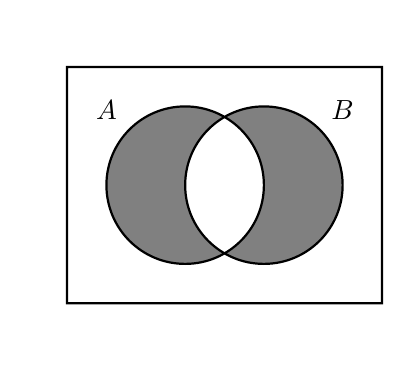
\begin{tikzpicture}[fill=gray]
% left hand
\scope
\clip (-2,-2) rectangle (2,2)
      (1,0) circle (1);
\fill (0,0) circle (1);
\endscope
% right hand
\scope
\clip (-2,-2) rectangle (2,2)
      (0,0) circle (1);
\fill (1,0) circle (1);
\endscope
% outline
\draw[thick] (0,0) circle (1) (-1,.7)  node [text=black,above] {$A$}
      (1,0) circle (1) (2,.7)  node [text=black,above] {$B$}
      (-1.5,-1.5) rectangle (2.5,1.5);
\end{tikzpicture}
\end{center}

  \begin{answer}
    For example, $A \cup B \cap \bar{(A \cap B)}$.  Note that $\bar{A \cap B}$ would almost work, but also contain the area outside of both circles.
  \end{answer}

  

\question Find the cardinalities:
\begin{parts}
  \part Find $|A|$ when $A = \{4,5,6,\ldots,37\}$
  \part Find $|A|$ when $A = \{x \in \Z \st -2 \le x \le 100\}$
  \part Find $|A \cap B|$ when $A = \{x \in \N \st x \le 20\}$ and $B = \{x \in \N \st x \mbox{ is prime}\}$
\end{parts}

  \begin{answer}
      \begin{parts}
	  \part 34.
	  \part 103.
	  \part 8.
      \end{parts}
  \end{answer}


  
  
\question Let $A = \{a, b, c\}$.  Find $\pow(A)$.

  \begin{answer}
    $\pow(A) = \{\emptyset, \{a\}, \{b\}, \{c\}, \{a,b\}, \{a,c\}, \{b,c\}, \{a,b,c\}\}$.
  \end{answer}

  
  

\question Let $A = \{1,2,\ldots, 10\}$.  How many subsets of $A$ contain exactly one element (i.e., how many {\em singleton} subsets are there).  How many {\em doubleton} (containing exactly two elements) are there?

  \begin{answer}
      There are 10 singletons.  There are 45 doubletons (because $45 = 9+8+7+\cdots+2+1$).
  \end{answer}


  
  
\question Let $A = \{1,2,3,4,5,6\}$.  Find all sets $B \in \pow(A)$ which have the property $\{2,3,5\} \subseteq B$.

  \begin{answer}
      $\{2,3,5\}, \{1,2,3,5\}, \{2,3,4,5\}, \{2,3,5,6\}, \{1,2,3,4,5\}, \{1,2,3,5,6\}, \{2,3,4,5,6\}$, and $\{1,2,3,4,5,6\}$.
  \end{answer}


  
\question Find an example of sets $A$ and $B$ such that $|A| = 4$, $|B| = 5$ and $|A \cup B| = 9$.  

  \begin{answer}
   For example $A = \{1,2,3,4\}$ and $B = \{5,6,7,8,9\}$.
  \end{answer}

  
  

\question Find an example of sets $A$ and $B$ such that $|A| = 3$, $|B| = 4$ and $|A \cup B| = 5$.

  \begin{answer}
    For example, $A = \{1,2,3\}$ and $B = \{2,3,4,5\}$.
  \end{answer}



\question In a regular deck of playing cards there are 26 red cards and 12 face cards.  Explain in terms of sets why there are only 32 cards which are either red or a face card.

  \begin{answer}
      If $R$ is the set of red cards and $F$ is the set of face cards, we want to find $|R \cup F|$.  This is not simply $|R| + |F|$ because there are 6 cards which are both red and a face card; $|R \cap F| = 6$.  We find $|R \cup F| = 32$.
  \end{answer}


  
% \question A group of college students were asked about their TV watching habits.  Of those surveyed, 28 students watch {\em House}, 19 watch {\em Castle} and 24 watch re-runs of {\em 24}.  Additionally, 16 watch {\em House} and {\em Castle}, 14 watch {\em House} and {\em 24} and 10 watch {\em Castle} and {\em 24}.  There are 8 students who watch all three shows.  How many students surveyed watched at least one of the shows?
% 
%   \begin{answer}
%     39.
%   \end{answer}
% 
% 
% 
% \question Find $|(A \cup C)\cap \bar B|$ provided $|A| = 50$, $|B| = 45$, $|C| = 40$, $|A\cap B| = 20$, $|A \cap C| = 15$, $|B \cap C| = 23$ and $|A \cap B \cap C| = 12$.
% 
%     \begin{answer}
%       $|(A \cup C)\cap \bar B| = 44$
%     \end{answer}
% 
% 
% 
% \question Using the same data as the previous question, describe a set with cardinality 26.
% 
%     \begin{answer}
% 	One possibility: $(A \cup B) \cap C$.
%     \end{answer}



  

% \question Consider the statement ``for all integers $a$ and $b$, if $a + b$ is even, then $a$ and $b$ are even''
% \begin{parts}
%  \part Write the contrapositive of the statement
%  \part Write the converse of the statement
%  \part Write the negation of the statement.
%  \part Is the original statement true or false?  Prove your answer.
%  \part Is the contrapositive of the original statement true or false?  Prove your answer.
%  \part Is the converse of the original statement true or false?  Prove your answer.
%  \part Is the negation of the original statement true or false?  Prove your answer.
% \end{parts}
% 
%   \begin{answer}
%     \begin{parts}
% 	\part For all integers $a$ and $b$, if $a$ or $b$ are not even, then $a+b$ is not even.
% 	\part For all integers $a$ and $b$, if $a$ and $b$ are even, then $a+b$ is even.
% 	\part There are numbers $a$ and $b$ such that $a+b$ is even but $a$ and $b$ are not both even.
% 	\part False.  For example, $a = 3$ and $b = 5$.  $a+b = 8$, but neither $a$ nor $b$ are even.
% 	\part False, since it is equivalent to the original statement.
% 	\part True.  Let $a$ and $b$ be integers.  Assume both are even.  Then $a = 2k$ and $b = 2j$ for some integers $k$ and $j$.  But then $a+b = 2k + 2j = 2(k+j)$ which is even.
% 	\part True, since the statement is false.
%       \end{parts}
%   \end{answer}
% 
% 
%   
%   
% \question Prove that $\sqrt 3$ is irrational.
% 
%   \begin{answer}
%     \begin{proof}
%      Suppose $\sqrt{3}$ were rational.  Then $\sqrt{3} = \frac{a}{b}$ for some integers $a$ and $b \ne 0$.  Without loss of generality, assume $\frac{a}{b}$ is reduced.  Now
% \[3 = \frac{a^2}{b^2}\]
% \[b^2 3 = a^2\]
% So $a^2$ is a multiple of 3.  This can only happen if $a$ is a multiple of 3, so $a = 3k$ for some integer $k$.  Then we have
% \[b^2 3 = 9k^2\]
% \[b^2 = 3k^2\]
% So $b^2$ is a multiple of 3, making $b$ a multiple of 3 as well.  But this contradicts our assumption that $\frac{a}{b}$ is in lowest terms.
%     \end{proof}
%   \end{answer}

 
 
 
  
% \question Translate into symbols.  Use $E(x)$ for ``$x$ is even'' and $O(x)$ for ``$x$ is odd.''
%  \begin{parts}
%   \part No number is both even and odd.
% \part One more than any even number is an odd number.
% \part There is prime number that is even.
% \part Between any two numbers there is a third number.
% \part There is no number between a number and one more than that number.
%  \end{parts}
% 
%   \begin{answer}
%      \begin{parts}
% 	\part $\neg \exists x (E(x) \wedge O(x))$
% 	\part $\forall x (E(x) \imp O(x+1))$
% 	\part $\exists x(P(x) \wedge E(x))$ (where $P(x)$ means ``$x$ is prime'')
% 	\part $\forall x \forall y \exists z(x < z < y \vee y < z < x)$
% 	\part $\forall x \neg \exists y (x < y < x+1)$
%     \end{parts}
%   \end{answer}
% 
%   
%  
%  
% \question Translate into English:
% \begin{parts}
%  \part $\forall x (E(x) \imp E(x +2))$
% \part $\forall x \exists y (\sin(x) = y)$
% \part $\forall y \exists x (\sin(x) = y)$
% \part $\forall x \forall y (x^3 = y^3 \imp x = y)$
% \end{parts}
% 
%   \begin{answer}
%     \begin{parts}
% 	\part Any even number plus 2 is an even number.
% 	\part For any $x$ there is a $y$ such that $\sin(x) = y$.  In other words, every number $x$ is in the domain of sine. 
% 	\part For every $y$ there is an $x$ such that $\sin(x) = y$.  In other words, every number $y$ is in the range of sine (which is false).
% 	\part For any numbers, if the cubes of two numbers are equal, then the numbers are equal.
%       \end{parts}
%   \end{answer}
% 
%   
%   
% 
% \question Simplify the statements (so negation appears only directly next to predicates).
% \begin{parts}
%   \part $\neg \exists x \forall y (\neg O(x) \vee E(y))$
%   \part $\neg \forall x \neg \forall y \neg(x < y \wedge \exists z (x < z \vee y < z))$
%   \part There is a number $n$ for which no other number is either less $n$ than or equal to $n$.
%   \part It is false that for every number $n$ there are two other numbers which $n$ is between.
% \end{parts}
% 
%   \begin{answer}
%     \begin{parts}
% 	\part $\forall x \exists y (O(x) \wedge \neg E(y))$
% 	\part $\exists x \forall y (x \ge y \vee \forall z (x \ge z \wedge y \ge z))$
% 	\part There is a number $n$ for which every other number is strictly greater than $n$.
% 	\part There is a number $n$ which is not between any other two numbers.
%       \end{parts}
%   \end{answer}
% 
%   
% 
% 
% \question Consider the statement ``for all integers $a$ and $b$, if $a + b$ is even, then $a$ and $b$ are even''
% \begin{parts}
%  \part Write the contrapositive of the statement
%  \part Write the converse of the statement
%  \part Write the negation of the statement.
%  \part Is the original statement true or false?  Prove your answer.
%  \part Is the contrapositive of the original statement true or false?  Prove your answer.
%  \part Is the converse of the original statement true or false?  Prove your answer.
%  \part Is the negation of the original statement true or false?  Prove your answer.
% \end{parts}
% 
%   \begin{answer}
%     \begin{parts}
% 	\part For all integers $a$ and $b$, if $a$ or $b$ are not even, then $a+b$ is not even.
% 	\part For all integers $a$ and $b$, if $a$ and $b$ are even, then $a+b$ is even.
% 	\part There are numbers $a$ and $b$ such that $a+b$ is even but $a$ and $b$ are not both even.
% 	\part False.  For example, $a = 3$ and $b = 5$.  $a+b = 8$, but neither $a$ nor $b$ are even.
% 	\part False, since it is equivalent to the original statement.
% 	\part True.  Let $a$ and $b$ be integers.  Assume both are even.  Then $a = 2k$ and $b = 2j$ for some integers $k$ and $j$.  But then $a+b = 2k + 2j = 2(k+j)$ which is even.
% 	\part True, since the statement is false.
%       \end{parts}
%   \end{answer}
% 
% 
%   
%   
% \question Prove that $\sqrt 3$ is irrational.
% 
%   \begin{answer}
%     \begin{proof}
%      Suppose $\sqrt{3}$ were rational.  Then $\sqrt{3} = \frac{a}{b}$ for some integers $a$ and $b \ne 0$.  Without loss of generality, assume $\frac{a}{b}$ is reduced.  Now
% \[3 = \frac{a^2}{b^2}\]
% \[b^2 3 = a^2\]
% So $a^2$ is a multiple of 3.  This can only happen if $a$ is a multiple of 3, so $a = 3k$ for some integer $k$.  Then we have
% \[b^2 3 = 9k^2\]
% \[b^2 = 3k^2\]
% So $b^2$ is a multiple of 3, making $b$ a multiple of 3 as well.  But this contradicts our assumption that $\frac{a}{b}$ is in lowest terms.
%     \end{proof}
%   \end{answer}
% 
%  
 
 
\end{questions}




%%
\begin{questions}
\question Make a truth table for the statement $(P \vee Q) \imp (P \wedge Q)$. 

\begin{answer}
 \begin{tabular}{c|c|c}
             $P$ & $Q$ & $(P \vee Q) \imp (P \wedge Q)$\\ \hline
             T & T & T \\
             T & F & F \\
             F & T & F \\
             F & F & T
          \end{tabular}
\end{answer}


\question Make a truth table for the statement $\neg P \wedge (Q \imp P)$.  What can you conclude about $P$ and $Q$ if you know the statement is true?

    \begin{answer}
      \begin{tabular}{c|c|c}
             $P$ & $Q$ & $\neg P \wedge (Q \imp P)$\\ \hline
             T & T & F \\
             T & F & F \\
             F & T & F \\
             F & F & T
          \end{tabular}
	If the statement is true, then both $P$ and $Q$ are false.
    \end{answer}


\question Make a truth table for the statement $\neg P \imp (Q \wedge R)$.

  \begin{answer}
    Hint: Like above, only now you will need 8 rows instead of just 4.
  \end{answer}


\question Determine whether the following two statements are logically equivalent: $\neg(P \imp Q)$ and $P \wedge \neg Q$.  Explain how you know you are correct.

  \begin{answer}
    Make a truth table for each and compare.  The statements are logically equivalent.
  \end{answer}

  
  

\question Are the statements $P \imp (Q\vee R)$ and $(P \imp Q) \vee (P \imp R)$ logically equivalent?

  \begin{answer}
    Again, make two truth tables.  The statements are logically equivalent.
  \end{answer}


  
  
\question Determine if the following argument form is valid: \begin{tabular}{rc} & $P \vee Q$ \\ & $\neg P$ \\ \hline $\therefore$ & $Q$\end{tabular}.

  \begin{answer}
    The argument is valid.  To see this, make a truth table which contains $P \vee Q$ and $\neg P$ (and $P$ and $Q$ of course).  Look at the truth value of $Q$ in each of the rows that have $P \vee Q$ and $\neg P$ true.  
  \end{answer}

  
  
  
\question Determine if the following argument form is valid: \begin{tabular}{rc} & $P \imp (Q \vee R)$ \\ & $\neg(P \imp Q)$ \\ \hline $\therefore$ & $R$\end{tabular}

  \begin{answer}
    The argument form is valid.  Again, make a truth table containing the premises and conclusion - look at the rows for which the premises are true.
  \end{answer}


  
\question Determine if the following argument form is valid: \begin{tabular}{rc} & $(P \wedge Q) \imp R$ \\ & $\neg P \vee \neg Q$ \\ \hline $\therefore$ & $\neg R$\end{tabular}

  \begin{answer}
    The argument is NOT valid.  If you make a truth table containing the premises and conclusion, there will be a row with both premises true but the conclusion false.  For example, if $P$ and $Q$ are false and $R$ is true, then $P \wedge Q$ is false, so $(P \wedge Q) \imp R$ is true.  Also $\neg P$ is true, so $\neg P \vee \neg Q$ is true.  However, $\neg R$ is false.
  \end{answer}


  
\question Consider the statement about a party, ``If it's your birthday or there will be cake, then there will be cake.''
\begin{parts}
 \part Translate the above statement into symbols.  Clearly state which statement is $P$ and which is $Q$.
 \part Make a truth table for the statement.
 \part Assuming the statement is true, what (if anything) can you conclude if there will be cake?
 \part Assuming the statement is true, what (if anything) can you conclude if there will not be cake?
 \part Suppose you found out that the statement was a lie.  What can you conclude?
\end{parts}

  \begin{answer}
    \begin{parts}
      \part $P$: it's your birthday; $Q$: there will be cake.  $(P \vee Q) \imp Q$
      \part Hint: you should get three T's and one F.
      \part Only that there will be cake.
      \part It's NOT your birthday!
      \part It's your birthday, but the cake is a lie.
    \end{parts}
  \end{answer}


  
\question Suppose $P$ and $Q$ are the statements:
$P$: Jack passed math.
$Q$: Jill passed math.
\begin{parts}
 \part Translate ``Jack and Jill both passed math'' into symbols.
\part Translate ``If Jack passed math, then Jill did not'' into symbols.
\part Translate ``$P \vee Q$'' into English.
\part Translate ``$\neg(P \wedge Q) \imp Q$'' into English.
\part Suppose you know that if Jack passed math, then so did Jill.  What can you conclude if you know that:
\begin{subparts}
 \subpart Jill passed math?  
\subpart  Jill did not pass math?
\end{subparts}
\end{parts}

  \begin{answer}
    \begin{parts}
      \part $P \wedge Q$
      \part $P \imp \neg Q$
      \part Jack passed math or Jill passed math (or both).
      \part If Jack and Jill did not both pass math, then Jill did.
      \part 
	\begin{subparts}
	  \subpart Nothing else. 
	  \subpart  Jack did not pass math either.
	\end{subparts}
    \end{parts}
  \end{answer}



  
\question Geoff Poshingten is out at a fancy pizza joint, and decides to order a calzone.  When the waiter asks what he would like in it, he replies, ``I want either pepperoni or sausage, and if I have sausage, I must also include quail.  Oh, and if I have pepperoni or quail then I must also have ricotta cheese.''  
\begin{parts}
	\part Translate Geoff's order into logical symbols.
	\part The waiter knows that Geoff is either a liar or a truth-teller (so either everything he says is false, or everything is true).  Which is it?
	\part What, if anything, can the waiter conclude about the ingredients in Geoff's desired calzone?
\end{parts}

  \begin{answer}
    \begin{parts}
	\part Three statements: $P \vee S$, $S \imp Q$, $(P \vee Q) \imp R$.  You could also connect the first two with a $\wedge$.
	\part He cannot be lying about all three sentences, so he is telling the truth.
	\part No matter what, Geoff wants ricotta.  If he doesn't have quail, then he must have pepperoni but not sausage.
    \end{parts}
  \end{answer}


  
  
\question Consider the statement ``If Oscar eats Chinese food, then he drinks milk.''
\begin{parts}
 \part Write the converse of the statement.
 \part Write the contrapositive of the statement.
 \part Is it possible for the contrapositive to be false?  If it was, what would that tell you?
 \part Suppose the original statement is true, and that Oscar drinks milk.  Can you conclude anything (about his eating Chinese food)?  Explain.
 \part Suppose the original statement is true, and that Oscar does not drink milk.  Can you conclude anything (about his eating Chinese food)?  Explain.
\end{parts}

  \begin{answer}
    \begin{parts}
      \part If Oscar drinks milk, then he eats Chinese food.
      \part If Oscar does not drink milk, then he does not eat Chinese food.
      \part Yes.  The original statement would be false too.
      \part Nothing. The converse need not be true.
      \part He does not eat Chinese food. The contrapositive would be true.
    \end{parts}
  \end{answer}

  
  

\question Simplify the following statements (so that negation only appears right before variables).
\begin{parts}
  \part $\neg(P \imp \neg Q)$
  \part $(\neg P \vee \neg Q) \imp \neg (\neg Q \wedge R)$
  \part $\neg((P \imp \neg Q) \vee \neg (R \wedge \neg R))$
  \part It is false that if Sam is not a man then Chris is a woman, and that Chris is not a woman.
\end{parts}

  \begin{answer}
    \begin{parts}
      \part $P \wedge Q$ 
      \part $(P \vee Q) \vee (Q \wedge \neg R)$
      \part F.  Or $(P \wedge Q) \wedge (R \wedge \neg R)$ 
      \part Either Sam is a woman and Chris is a man, or Chris is a woman.
    \end{parts}
  \end{answer}


  
\question Which of the following statements are equivalent to the implication, ``if you win the lottery, then you will be rich,'' and which are equivalent to the converse of the implication?
\begin{parts}
 \part Either you win the lottery or else you are not rich.
 \part Either you don't win the lottery or else you are rich.
 \part You will win the lottery and be rich.
 \part You will be rich if you win the lottery.
 \part You will win the lottery if you are rich.
 \part It is necessary for you to win the lottery to be rich.
 
 \part It is sufficient to with the lottery to be rich.
 \part You will be rich only if you win the lottery.
 \part Unless you win the lottery, you won't be rich.
 \part If you are rich, you must have one the lottery.
 \part If you are not rich, then you did not win the lottery.
 \part You will win the lottery if and only if you are rich.
\end{parts}

  \begin{answer} The statements are equivalent to the\ldots
    \begin{parts}
      \part converse.
      \part implication.
      \part neither.
      \part implication.
      \part converse.
      \part converse.
      
      \part implication.
      \part converse.
      \part converse.
      \part converse (in fact, this IS the converse).
      \part implication (the statement is the contrapositive of the implication).
      \part neither.
    \end{parts}
  \end{answer}

  
\question Consider the implication, ``if you clean your room, then you can watch TV.''  Rephrase the implication in as many ways as possible.  Then do the same for the converse.

  \begin{answer}
    Hint: of course there are many answers.  It helps to assume that the statement is true and the converse is NOT true.  Think about what that means in the real world and then start saying it in different ways.  Some ideas: use necessary and sufficient language, use ``only if,'' consider negations, use ``or else'' language.
  \end{answer}

  
% \question Translate into symbols.  Use $E(x)$ for ``$x$ is even'' and $O(x)$ for ``$x$ is odd.''
%  \begin{parts}
%   \part No number is both even and odd.
% \part One more than any even number is an odd number.
% \part There is prime number that is even.
% \part Between any two numbers there is a third number.
% \part There is no number between a number and one more than that number.
%  \end{parts}
% 
%   \begin{answer}
%      \begin{parts}
% 	\part $\neg \exists x (E(x) \wedge O(x))$
% 	\part $\forall x (E(x) \imp O(x+1))$
% 	\part $\exists x(P(x) \wedge E(x))$ (where $P(x)$ means ``$x$ is prime'')
% 	\part $\forall x \forall y \exists z(x < z < y \vee y < z < x)$
% 	\part $\forall x \neg \exists y (x < y < x+1)$
%     \end{parts}
%   \end{answer}
% 
%   
%  
%  
% \question Translate into English:
% \begin{parts}
%  \part $\forall x (E(x) \imp E(x +2))$
% \part $\forall x \exists y (\sin(x) = y)$
% \part $\forall y \exists x (\sin(x) = y)$
% \part $\forall x \forall y (x^3 = y^3 \imp x = y)$
% \end{parts}
% 
%   \begin{answer}
%     \begin{parts}
% 	\part Any even number plus 2 is an even number.
% 	\part For any $x$ there is a $y$ such that $\sin(x) = y$.  In other words, every number $x$ is in the domain of sine. 
% 	\part For every $y$ there is an $x$ such that $\sin(x) = y$.  In other words, every number $y$ is in the range of sine (which is false).
% 	\part For any numbers, if the cubes of two numbers are equal, then the numbers are equal.
%       \end{parts}
%   \end{answer}
% 
%   
%   
% 
% \question Simplify the statements (so negation appears only directly next to predicates).
% \begin{parts}
%   \part $\neg \exists x \forall y (\neg O(x) \vee E(y))$
%   \part $\neg \forall x \neg \forall y \neg(x < y \wedge \exists z (x < z \vee y < z))$
%   \part There is a number $n$ for which no other number is either less $n$ than or equal to $n$.
%   \part It is false that for every number $n$ there are two other numbers which $n$ is between.
% \end{parts}
% 
%   \begin{answer}
%     \begin{parts}
% 	\part $\forall x \exists y (O(x) \wedge \neg E(y))$
% 	\part $\exists x \forall y (x \ge y \vee \forall z (x \ge z \wedge y \ge z))$
% 	\part There is a number $n$ for which every other number is strictly greater than $n$.
% 	\part There is a number $n$ which is not between any other two numbers.
%       \end{parts}
%   \end{answer}
% 
%   
% 
% 
% \question Consider the statement ``for all integers $a$ and $b$, if $a + b$ is even, then $a$ and $b$ are even''
% \begin{parts}
%  \part Write the contrapositive of the statement
%  \part Write the converse of the statement
%  \part Write the negation of the statement.
%  \part Is the original statement true or false?  Prove your answer.
%  \part Is the contrapositive of the original statement true or false?  Prove your answer.
%  \part Is the converse of the original statement true or false?  Prove your answer.
%  \part Is the negation of the original statement true or false?  Prove your answer.
% \end{parts}
% 
%   \begin{answer}
%     \begin{parts}
% 	\part For all integers $a$ and $b$, if $a$ or $b$ are not even, then $a+b$ is not even.
% 	\part For all integers $a$ and $b$, if $a$ and $b$ are even, then $a+b$ is even.
% 	\part There are numbers $a$ and $b$ such that $a+b$ is even but $a$ and $b$ are not both even.
% 	\part False.  For example, $a = 3$ and $b = 5$.  $a+b = 8$, but neither $a$ nor $b$ are even.
% 	\part False, since it is equivalent to the original statement.
% 	\part True.  Let $a$ and $b$ be integers.  Assume both are even.  Then $a = 2k$ and $b = 2j$ for some integers $k$ and $j$.  But then $a+b = 2k + 2j = 2(k+j)$ which is even.
% 	\part True, since the statement is false.
%       \end{parts}
%   \end{answer}
% 
% 
%   
%   
% \question Prove that $\sqrt 3$ is irrational.
% 
%   \begin{answer}
%     \begin{proof}
%      Suppose $\sqrt{3}$ were rational.  Then $\sqrt{3} = \frac{a}{b}$ for some integers $a$ and $b \ne 0$.  Without loss of generality, assume $\frac{a}{b}$ is reduced.  Now
% \[3 = \frac{a^2}{b^2}\]
% \[b^2 3 = a^2\]
% So $a^2$ is a multiple of 3.  This can only happen if $a$ is a multiple of 3, so $a = 3k$ for some integer $k$.  Then we have
% \[b^2 3 = 9k^2\]
% \[b^2 = 3k^2\]
% So $b^2$ is a multiple of 3, making $b$ a multiple of 3 as well.  But this contradicts our assumption that $\frac{a}{b}$ is in lowest terms.
%     \end{proof}
%   \end{answer}
% 
%  
 
 
\end{questions}




%\documentclass[12pt]{article}

\usepackage{../discrete}

\heading{Math 228}{}{Logic 2: Quantifiers and Sets Notes }



\begin{document}
\section*{Quantifiers and Sets}

So far we have seen how statements can be combined with logical symbols.  This is helpful when trying to understand a complicated mathematical statement - you can determine under which conditions the complicated statement is true.  Additionally, we have been able to analyze the logical form of arguments to decide which arguments are valid and which are not.  However, the types of statements we have been able to make so far has be sorely limited.  For example, consider a classic argument:

\begin{center}
 All men are mortal.\\ Socrates is a man. \\
 Therefore, Socrates is mortal.
\end{center}

This is clearly a valid argument - it is an example of a {\em syllogism}.  Historically, the study of logic began with Aristotle who worked out all possible forms of syllogisms and decided which were valid and which were not.  We will not do that here.  However, this is an important example because it highlights a limitation of the propositional logic we have studied so far.  Can we use propositional logic to analyze the argument?  

The trouble is that we don't have a way to translate ``all men are mortal.''  It looks like an implication - being a man implies you are mortal.  So maybe it is $P \imp Q$.  But what is $P$?  We could rephrase: ``if Socrates is a man, then Socrates is mortal.''  Now we have a valid argument form we have seen before.  But it is not quite the same.  (What if the argument was: All men are mortal, all mortals have hair, therefore all men have hair - also valid and Socrates has nothing to do with it.)  Or perhaps we could go with, ``for every thing there is, if the thing is a man, then the thing is mortal.''  Looks promising, but we still can't let $P$ be ``the thing is a man'' - that is not a statement because ``thing'' is a variable.

One way to sort this mess out is to introduce a new sort of logic called {\em predicate} logic.  This is the logic of properties.  Doing so will allow us to discuss how properties of various things are related.  Above, if a thing has the property of being a man, then it has the property of being mortal.  We can then {\em quantify} over what things we talk about.  The the example above, {\em all} things.  

Another way to accomplish much of the same goal is to use set theory.  This will also be useful in solving other types of problems later on.  The idea here is that we want talk about collections of things - for example, the collection of all men, and the collection of all mortal things.  We can then express ``all men are mortal'' by saying that the set of men is a subset of the set of mortals.  Then we claim that Socrates is a member of the set of men, so therefore is also a member of the set of mortals.

One last example to highlight these two different approaches before delving into the details of each.  We all agree that all squares are rectangles.  The set theory approach would be to consider the set of squares and the set of rectangles, and point out that one is a subset of the other (the squares are a subset of the rectangles).  The predicate logic approach would be to consider the properties of ``being a square'' and of ``being a rectangle'' and assign these to predicates - say $S$ and $R$.  We would then say $\forall x (S(x) \imp R(x))$ - for all things, if the thing is a square, then it is a rectangle.  So having the property of being a square implies having the property of being a rectangle.

Now some details.




\section{Quantifiers and Predicate Logic}

Consider the statement ``for all integers $a$ and $b$, if $ab$ is even, then $a$ is even or $b$ is even.''  If we use propositional logic to analyze this statement, what should $P$ be?  

You might want to say $P$ is ``$ab$ is even'' so $Q$ can be ``$a$ is even'' and $R$ can be ``$b$ is even'' and say that the whole statement is therefore of the form $P \imp (Q \vee R)$.  This does not work!  One reason is that ``$ab$ is even'' is not a statement - it contains free variables, so it is not true or false (until the variables have values).  Another reason is that we have just lost the ``for all integers $a$ and $b$'' from our statement.  We can remedy both these problems using {\em Predicate Logic}.

\subsection{Predicates}

We can think of predicates as properties of objects.  For example, consider the predicate $E$ which we will use to mean ``is even.''  Being even is a property of some numbers, so $E$ needs to be applied to something.  We will adopt the notation $E(x)$ to mean $x$ is even.  (Some books would write $Ex$ instead.)  Notice that if we put a number in for $x$, then this becomes a statement - and as such can be true or false.  So $E(2)$ is true, and $E(3)$ is false.  On the other hand $E(x)$ is not true or false, since we don't know what $x$ is.  If we have a variable floating around like that, we say the expression is merely a formula, and not a statement.

Since $E(2)$ is a statement (a proposition), we can apply propositional logic to it.  Consider 
\[E(2) \wedge \neg E(3)\]
which is a true statement, because it is both the case that 2 is even and that 3 is not even.  What we have done here is capture the logical form (using connectives) of the statement ``2 is even and 3 is not'' as well as the mathematical content (using predicates).

Notice that we can only assert even-ness of a single number at a time.  That is to say, $E$ is a {\em one-place} predicate.  There are also predicates which assert a property of two or more numbers (or other objects) at the same time.  Consider the {\em two-place} predicate ``is less than.''  Perhaps we will use the variable $L$.  Now we can say $L(2,3)$, which is true because 2 is less than 3.  Of course we are already have a symbol for this: $2 < 3$.  However, what about ``divides evenly into'' as a predicate?  We can say $D(2,10)$ is true because 2 divides evenly into 10, while $D(3, 10)$ is false since there is a remainder when you divide 10 by 3.  Incidentally, there is a standard mathematical symbol for this: $2 | 10$ is read ``2 divides 10.''  

Predicates can be as complicated and have as many places as we want or need.  For example, we could $R(x,y,z,u,v,w)$ be the predicate asserting that $x$, $y$, $z$ are distinct natural numbers whose only common factor is $u$, the difference between $x$ and $y$ is $v$ and the difference between $y$ and $z$ is $w$.  This is a silly and most likely useless example, but it is an example of a predicate.  It is true of some ordered lists of six numbers (6-tuples), and false of others.  Additionally, predicates need not have anything to do with numbers: we could let $F(a,b,c,d)$ be the predicate that asserts that $a$ and $b$ are the only two children of mother $c$ and father $d$.

\subsection{Quantifiers}

Perhaps the most important reason to use predicate logic is that doing so allows for quantification.  We can now express statements like ``ever natural number is either even or odd,'' and ``there is a natural number such that no number is less than it.''  Think back to Calculus and the Mean Value Theorem.  It states that for every function $f$ and every interval $(a, b)$, if $f$ is continuous on the interval $[a,b]$ and differentiable on the interval $(a,b)$, then there exists a number $c$ such that $a \le c \le b$ and $f'(c)(b - a) = f(b) - f(a)$.  Using the correct predicates and quantifiers, we could express this statement entirely in symbols.  

There are two quantifiers we will be interested in: existential and universal.  

\begin{defbox}{Quantifiers}
  \begin{itemize}
    \item The existential quantifier is $\exists$ and is read ``there exists'' or ``there is.''  For example,
\[\exists x (x < 0)\]
asserts that there is a number less than 0.
\item The universal quantifier is $\forall$ and is read ``for all'' or ``every.''  For example,
\[\forall x (x \ge 0)\]
asserts that every number is greater than or equal to 0.
  \end{itemize}    
\end{defbox}

  Are these statements true?  Well, first notice that they cannot both be true.  In fact, they assert exactly the opposite of each other.  (Note that $x < y \iff \neg(x \ge y)$ -- although you might wonder what $x$ and $y$ are here, so it might be better to say $\forall x \forall y\left(x < y \iff \neg(x \ge y)\right)$.)  Which one is it though?  The answer depends entirely on our domain of discourse - the universe over which we quantify.  Usually, this universe is clear from the context.  If we are only discussing the natural numbers, then $\forall x \ldots$ means ``for every natural number $x \ldots$.''  On the other hand, in calculus we care about the real numbers, so it would mean ``for every real number $x \ldots$.''  If the context is not clear, we might right $\forall x \in \N\ldots$ to mean ``for every natural number $x\ldots$.''  Of course, for the two statements above, the second is true of the natural numbers, the first is true for any larger universe.\footnote{In this class we take the natural 
numbers to be 0, 1, 2, 3, \ldots}

Some more examples: to say ``every natural number is either even or odd,'' we would write, using $E$ and $O$ as the predicates for even and odd respectively:
\[\forall x (E(x) \vee O(x))\]
To say ``there is a number such that no number is less than it'' we would write:
\[ \exists x \forall y (y \ge x)\]
Actually, I did a little translation before I wrote that down.  The above statement would be literally read ``there is a number such that every number is greater than or equal to it.''  This of course amounts to the same thing.  However, if I wanted to be exact, I could have also written:
\[ \exists x \neg \exists y (y < x).\]
Notice also that say that there is a number for which no number is smaller is equivalent to saying that it is not the case that for every number there is a number smaller than it:
\[\neg \forall x \exists y (y < x).\]
That these three statements are equivalent is no coincidence.  To understand what is going on, we will need to better understand how quantification interacts with the logical connectives, specifically negation.

\subsection{Quantifiers and Connectives}

What does it mean to say that it is false that there is something that has a certain property?  Well, it means that everything does not have that property.  What does it mean for it to be false that everything has a certain property?  It means that there is something that doesn't have the property.  So in symbols, we have the following

\begin{defbox}{Quantifiers and Negation}
\[\neg \forall x P(x) \mbox{ is equivalent to } \exists x \neg P(x)\]
and
\[\neg \exists x P(x)\mbox{ is equivalent to } \forall x \neg P(x).\]
\end{defbox}

In other words, to move a negation symbol past a quantifier, you must switch the quantifier. This can be done multiple times:
\[\neg \exists x \forall y \exists z P(x,y,z) \mbox{ is equivalent to } \forall x \exists y \forall z \neg P(x,y,z).\]
Now we also know how to move negation symbols through other connectives (using De Morgan's Laws) so it is always possible to rewrite a statement so that the only negation symbols that appear are right in front of a predicate.  This hints at the possibility of having a standard form for all predicate statements.  However, to get this we must also understand how to move quantifiers through connectives.

Before we get too excited, note that we only need to worry about two connectives: $\wedge$ and $\vee$.  This is because we can rewrite $p \imp q$ as $\neg p \vee q$ (they are logically equivalent) and $p \iff q$ as $(p \wedge q) \vee (\neg p \wedge \neg q)$ (also logically equivalent).  

Let us consider an example to see what can happen.

\begin{example} 
  Let $E$ be the predicate for being even, and $O$ for being odd.  Consider:
\[\exists x E(x) \wedge \exists x O(x),\]
which says that there is a number which is even and a number which is odd.  This is of course true.  However there is no number which is both even and odd, so 
\[\exists x (E(x) \wedge O(x))\]
is false.  Note also that
\[\exists x (E(x) \vee O(x))\]
while true, is not really the same thing -- if $O$ is instead the predicate for ``is less than 0'' then the original statement is false, but this new one is true (of the natural numbers).  Changing the quantifier also doesn't help:
\[\forall x (E(x) \wedge O(x))\]
is false.  So what can we do?

The problem is that in the original sentence, the variable $x$ is doing double duty.  We want to express the fact that there is an even number and an odd number.  But that even number is in no way related to that odd number.  So we might as well have said
\[ \exists x E(x) \wedge \exists y O(y).\]
Now we can move the quantifiers out:
\[\exists x \exists y (E(x) \wedge O(y)).\]
\end{example}

The same thing works with $\vee$ and for $\forall$ with either connective.  As long as there is no repeat in quantified variables we can move the quantifiers outside of conjunctions and disjunctions.  

A warning though: you cannot do this for $\imp$, at least not directly.\footnote{We must be similarly careful with $\iff$}  Let's see what happens.  

\begin{example}
Consider
\[ \forall x P(x) \imp \exists y Q(y)\]
for some predicates $P$ and $Q$.  This sentence is {\bf not} the same as
\[ \forall x \exists y (P(x) \imp Q(y)).\]
Remember that $p \imp q$ is the same as $\neg p \vee q$.  So the original sentence is really
\[\neg \forall x P(x) \vee \exists y Q(y).\]
Before we move the quantifiers out, we must move the $\forall x$ past the negation sign, which switches it to a $\exists x$:
\[\exists x \neg P(x) \vee \exists y Q(y).\]
Then we can finish by writing,
\[\exists x \exists y (\neg P(x) \vee Q(y))\]
or equivalently
\[\exists x \exists y (P(x) \imp Q(y)).\]
\end{example}



\section{Sets and Set Notation}
For us, a set will simply be an unordered collection of objects.  For example, we could consider the set of all students enrolled at UNC this semester.  Or the set of natural numbers between 1 and 10 inclusive.  In the first case, each student here is a element (or member) of the set, while Barack Obama, among many others, is not an element of the set.  Also, the two example are of different sets.  Two sets are equal exactly if they contain the exact same elements.

Because we will want to consider many examples, we should have some notation to make talking about sets easier.  Consider,
\[ A = \{1, 2, 3\}.\]
This is read, ``$A$ is the set containing the elements 1, 2 and 3.''  We use curly braces ``$\{,~~ \}$'' to enclose elements of a set.  Some more notation:
\[ a \in \{a, b, c\}. \]
The symbol ``$\in$'' is read ``is in'' or ``is an element of.''  Thus the above means that $a$ is an element of the set containing the letters $a$, $b$, and $c$.  Note that this is a true statement.  It would also be true to say that $d$ is not in that set:
\[ d \not\in \{a, b, c\}.\]
Be warned: we say ``$x \in A$'' when we wish to express that ``one of the elements of the set $A$ is $x$.''  For example, consider the set,
\[A = \{1, b, \{x, y, z\}, \emptyset\}\]
This is a strange set, to be sure. It contains four elements: the number 1, the letter b, the set $\{x,y,z\}$ and the empty set ($\emptyset = \{ \}$, the set containing no elements).  Is $x$ in $A$?  The answer is no.  None of the four elements in $A$ are the letter $x$, so we must conclude that $x \notin A$.  Similarly, if we considered the set $B = \{1,b\}$, then again $B \notin A$ - even though the elements of $B$ are also elements of $A$, we cannot say that the thing $B$ is one of the things in the collection $A$. 

If a set is {\em finite}, then we can describe it by simply listing the elements.  Infinite sets exists though, so we need to be able to describe them as well.  For instance, if we want $A$ to be the set of all even natural numbers, would could write,
\[ A = \{2, 4, 6, \ldots\}\]
but this is a little imprecise.  Better would be
\[ A = \{x \in \N \st \exists n\in \N ( x = 2 n)\}.\]
Breaking that down: $x \in \N$ means $x$ is in the set $\N$ (the set of natural numbers), $\st$ is read ``such that'' and $\exists n (x = 2n)$ is read ``there exists an $n$ in the natural numbers for which $x$ is two times $n$'' (in other words, $x$ is even).  Slightly easier might be,
\[ A = \{x \st \mbox{ $x$ is even }\}. \]

Note: sometime people use $|$ for the ``such that'' symbol instead of $:$.


\begin{defbox}{Set Theory Notation}

\noindent  \begin{tabular}{l p{1.5in} p{3.5in}}
    Symbol: & Read: & Example: \\ \hline \\[1ex]
    $\{$, $\}$ & braces & $\{1,2,3\}$.  The braces enclose the elements of a set.  This is the set which contains the numbers 1, 2 and 3.\\[1ex]
    $\st$ & such that & $\{x \st x > 2\}$ is the set of all $x$ such that $x$ is greater than 2.\\[1ex]
    $\in$ & is an element of & $2 \in \{1,2,3\}$ asserts that 2 is one of the elements in the set $\{1,2,3\}$.  However, $4 \notin\{1,2,3\}$.\\[1ex]
    $\subseteq$ & is a subset of & $A \subseteq B$ asserts that every element of $A$ is also an element of $B$.\\[1ex]
    $\subset$ &is a proper subset of & $A \subset B$ asserts that every element of $A$ is also an element of $B$, but $A \ne B$.\\[1ex]
    $\cap$ & intersection & $A \cap B$ is the {\em set} of all elements which are elements of both $A$ and $B$.\\[1ex]
    $\cup$ & union & $A \cup B$ is the {\em set} of all elements which are elements of $A$ or $B$ or both.\\[1ex]
    $\setminus$ & set difference & $A \setminus B$ is the {\em set} of all elements of $A$ which are not elements of $B$.\\[1ex]
    $\bar A$ & compliment (of $A$) & $\bar A$ is the set of everything which is not an element of $A$.  The $A$ can be any set here.\\[1ex]
    $|A|$ & cardinality (of $A$)& $|\{4,5,6\}| = 3$ because there are 3 elements in the set.  Sometimes we say $|A|$ is the {\em size} of $A$.\\[1ex]
    
  \end{tabular}

\noindent{\bf Special sets}

\begin{tabular}{l p{5in}}
  $\emptyset$ & The {\em empty set} is the set which contains no elements.\\[1ex]
  $\U$ & The {\em universe set} is the set of all elements.\\[1ex]
$\N$ & The set of natural numbers. That is, $\N = \{0, 1, 2, 3\ldots\}$ \\[1ex]
$\Z$ & The set of integers.  $\Z = \{\ldots, -2, -1, 0, 1, 2, 3, \ldots\}$\\[1ex]
$\Q$ & The set of rational numbers.\\[1ex]
$\R$ & The set of real numbers.\\[1ex]
$\pow(A)$ & The {\em power set} of any set $A$ is the set of all subsets of $A$.
\end{tabular}
\end{defbox}


\subsection{Relationships between sets}

We have already said what it means for two sets to be equal: they have exactly the same elements.  Thus, for example,
\[ \{1, 2, 3\} = \{2, 1, 3\}.\]
(Remember, the order the elements are written down in does not matter.)  Also,
\[ \{1, 2, 3\} = \{I, II, III\}.\]
Now what about the sets $A = \{1, 2, 3\}$ and $B = \{1, 2, 3, 4\}$?  Clearly $A \ne B$.  However, we can notice that every element of $A$ is also an element of $B$.  Because of this, we say that $A$ is a subset of $B$, or in symbols $A \subset B$ or $A \subseteq B$.  (Both symbols are read ``is a subset of.'' The difference is that sometimes we want to say that $A$ is either equal to or a subset of $B$, in which case we use $\subseteq$.  Compare the difference between $<$ and $\le$.)

\begin{example}
 Let $A = \{1, 2, 3, 4, 5, 6\}$, $B = \{2, 4, 6\}$, $C = \{1, 2, 3\}$ and $D = \{7, 8, 9\}$.  Determine which of the following are true, false, or meaningless.
\begin{multicols}{3}
\begin{enumerate}
\item $A \subset B$
\item $B \subset A$
\item $B \in C$
\item $\emptyset \in A$
\item $\emptyset \subset A$
\item $A < D$
\item $3 \in C$
\item $3 \subset C$.
\item $\{3\} \subset C$
\end{enumerate}
\end{multicols}
\begin{solution}
 \begin{enumerate}
  \item False.
\item True: every element in $B$ is an element in $A$.
\item False: the elements in $C$ are 1, 2, and 3.  The {\em set} $B$ is not equal to 1, 2, or 3.
\item False: $A$ has exactly 6 elements, and none of them are the empty set.
\item True: Everything in the empty set (nothing) is also an element of $A$.  Notice that the empty set is a subset of every set.
\item Meaningless.  A set cannot be less that another set.
\item True.
\item Meaningless.  $3$ is not a set, so it cannot be a subset of another set.
\item True.  $3$ is the only element of the set $\{3\}$, and is an element of $C$, so every element in $\{3\}$ is an element of $C$.
 \end{enumerate}
\end{solution}
\end{example}

In the example above, $B$ is a subset of $A$.  You might wonder what other sets are subsets of $A$.  If you collect all these subsets of $A$, they themselves for a set - a set of sets.  We call the set of all subsets of $A$ the {\em power set} of $A$, and write it $\pow(A)$.  

\begin{example}
  Let $A = \{1,2,3\}$.  Find $\pow(A)$.
  \begin{solution}
    $\pow(A)$ is a set of sets - all of which are subsets of $A$.  So
    \[\pow(A) = \{ \emptyset, \{1\}, \{2\}, \{3\}, \{1,2\}, \{1, 3\}, \{2,3\}, \{1,2,3\}\}\]
    Notice that while $2 \in A$, it is wrong to write $2 \in \pow(A)$ - none of the elements in $\pow(A)$ are numbers!.  On the other hand we do have $\{2\} \in \pow(A)$ because $\{2\} \subseteq A$.  
    
    What does a subset of $\pow(A)$ look like?  Notice that $\{2\} \not\subseteq \pow(A)$ because not everything in $\{2\}$ is in $\pow(A)$.  But we do have $\{ \{2\} \} \subseteq \pow(A)$.  The only element of $\{\{2\}\}$ is the set $\{2\}$ which is also an element of $\pow(A)$.  We could take the collection of all subsets of $\pow(A)$ and call that $\pow(\pow(A))$.  Or even the power set of that set of sets of sets. 
  \end{solution}

\end{example}


Another way to compare sets is by their size.  Notice that in the example above, $A$ has 6 elements, $B$, $C$, and $D$ all have 3 elements.  The size of a set is called the set's cardinality.  We would write $|A| = 6$, $|B| = 3$ and so on.  For sets that have a finite number of elements, the cardinality of the set is simply the number of elements in the set.  Note that the cardinality of $\{ 1, 2, 3, 2, 1\}$ is 3 -- we do not count repeats (in fact, $\{1, 2, 3, 2, 1\}$ is exactly the same set as $\{1, 2, 3\}$).  There are sets with infinite cardinality, such as $\N$, the set of rational numbers (written $\mathbb Q$), the set of even natural numbers, the set of real number ($\mathbb R$).  It is possible to distinguish between different infinite cardinalities, but that is beyond the scope of these notes.  For us, a set will either be infinite, or finite, and if it is finite, we can determine it's cardinality by counting elements.

\begin{example}
 Find the cardinality of $\{23, 24, \ldots, 37, 38\}$.  
\begin{solution}
 Since $38 - 23 = 15$, we can conclude that the cardinality of the set is 16 (you need to add one since 23 is included).
\end{solution}
\end{example}

\subsection{Operations on sets}

Is it possible to add two sets?  Not really, however there is something similar.  If we want to combine two sets -- to get the collection of objects that are in either set, then we can take the {\em union} of the two sets.  Symbolically,
\[ C = A \cup B\]
means $C$ is the union of $A$ and $B$.  Every element of $C$ is either an element of $A$ or an element of $B$ (or an element of both).  For example, if $A = \{1, 2, 3\}$ and $B = \{2, 3, 4\}$, then $A \cup B = \{1, 2, 3, 4\}$.

The other common operation on sets is {\em intersection}.  We write,
\[ C = A \cap B\]
to mean that $C$ is the intersection of $A$ and $B$; everything in $C$ is in both $A$ and in $B$.  So if $A = \{1, 2, 3\}$ and $B = \{2, 3, 4\}$, then $A \cap B = \{2, 3\}$.  

Often when dealing with sets, we will have some understanding as to what ``everything'' is.  Perhaps we are only concerned with natural numbers.  We would say that our {\em universe} is $\N$.  Sometimes we call denote this universe by $\U$.  Given this context, we might wish to speak of all the elements which are {\em not} in a particular set.  We call this the {\em compliment} of the set, and write,
\[ B = \bar A\]
when $B$ contains every element not contained in $A$.  So if our universe is $\{1, 2,\ldots, 9, 10\}$, and $A = \{2, 3, 5, 7\}$, then $\bar A = \{1, 4, 6, 8, 9,10\}$.

Of course we can perform more than one operation at a time.  Fore example, consider
\[A \cap \bar B\]
This is the set of all element which are both elements of $A$ and not elements of $B$.  What have we done?  We've started with $A$ and removed all of the elements which were in $B$.  Another way to write this is the {\em set difference}:
\[A \cap \bar B = A \setminus B\]

It is important to remember that these operations (union, intersection, compliment and difference) on sets produce other sets.  Don't confuse these with the symbols from the previous section (element of and subset of).  $A \cap B$ is a set, while $A \subseteq B$ is true or false.  This is the same difference as between $3 + 2$ (which is a number) and $3 \le 2$ (which is in this case false).

\begin{example}
 Let $A = \{1, 2, 3, 4, 5, 6\}$, $B = \{2, 4, 6\}$, $C = \{1, 2, 3\}$ and $D = \{7, 8, 9\}$.  The universe is $\U = \{1, 2, \ldots, 10\}$.  Find:
\begin{multicols}{3}
 \begin{enumerate}
  \item $A \cup B$
\item $A \cap B$
\item $B \cap C$
\item $A \cap D$
\item $\bar{B \cup C}$
\item $A \cap \bar B$
\item $(D \cap \bar C) \cup \bar{A \cap B}$
\item $\emptyset \cup C$
\item $\emptyset \cap C$
 \end{enumerate}
\end{multicols}
\begin{solution}
  \begin{enumerate}
  \item $A \cup B = \{1, 2, 3, 4, 5, 6\} = A$ since everything in $B$ is already in $A$.
\item $A \cap B = \{2, 4, 6\} = B$ since everything in $B$ is in $A$.
\item $B \cap C = \{2\}$ - the only element of both $B$ and $C$ is 2.
\item $A \cap D = \emptyset$ since $A$ and $D$ have no common elements
\item $\bar{B \cup C} = \{5, 7, 8, 9, 10\}$.  First we find that $B \cup C = \{1, 2, 3, 4, 6\}$, then we take everything not in that set.
\item $A \cap \bar B = \{1, 3, 5\}$.  Everything that is in $A$ which is not in $B$.  This is the same as $A \setminus B$.
\item $(D \cap \bar C) \cup \bar{A \cap B} = \{1, 3, 5, 7, 8, 9\}.$ The set contains all elements that are either in $D$ but not in $C$ or not in both $A$ and $B$.
\item $\emptyset \cup C = C$ - nothing is added by the emptyset.
\item $\emptyset \cap C = \emptyset$ - nothing can be both in a set and in the emptyset.
 \end{enumerate}
\end{solution}
\end{example}

You might notice that the symbols for union and intersection slightly resemble the logic symbols for ``or'' and ``and.''  This is no accident.  What does it mean for $x$ to be an element of $A\cup B$?  It means that $x$ is an element of $A$ or $x$ is an element of $B$ (or both).  That is,
\[x \in A \cup B \qquad \Iff \qquad x \in A \vee x \in B.\]
Similarly,
\[x \in A \cap B \qquad \Iff \qquad x \in A \wedge x \in B.\]
Also,
\[x \in \bar A \qquad \Iff \qquad \neg (x \in  A)\]
which says $x$ is an element of the compliment of $A$ if $x$ is not an element of $A$.

Given all this, you should not be surprised to find out that there is a version of De Morgan's laws for sets:

\begin{defbox}{De Morgan's Laws (for sets)}
  For any sets $A$ and $B$ in some universe $\U$:
  \[\bar{A \cap B} = \bar A \cup \bar B\]
  \[\bar{A \cup B} = \bar A \cap \bar B\]
\end{defbox}

Do you believe these equations?  To check De Morgan's laws in logic we could just make a truth table for each statement.  We don't have truth tables for sets, but we do have\ldots.

\subsection{Venn Diagrams}
Union, intersection, compliment, set difference - operations can get complicated (see part 7 in the above example).  Luckily, there is a very nice visual tool we can use to clarify things.  Venn diagrams represent sets as intersecting circles.  We can shade the region we are talking about when we carry out an operation.  We can also represent cardinality of a particular set by putting the number in the corresponding region.\\

\begin{center}
\begin{tikzpicture}[fill=gray!50]
 \draw[thick] \circleA \circleAlabel \circleB \circleBlabel \twosetbox;
\end{tikzpicture} \hspace{2in}
\begin{tikzpicture}[scale=.75, fill=gray!50]
 \draw[thick] \circleA \circleAlabel \circleB \circleBlabel \circleC \circleClabel \threesetbox;
\end{tikzpicture}\\
\end{center}

%\includegraphics[width=2in]{images/venn2blank.png} \hfill \includegraphics[width=2in]{images/venn3blank.png}\\

Each circle represents a set.  The rectangle containing the circles represents the universe.  To represent combinations of these sets, we shade the corresponding region.  For example, we could draw $A \cap B$ as:

\begin{center}
\begin{tikzpicture}[fill=gray!50]
	\begin{scope}
	\clip \circleA;
	\fill \circleB;
	\end{scope}
 \draw[thick] \circleA \circleAlabel \circleB \circleBlabel \twosetbox;
\end{tikzpicture}

%  \includegraphics[width=2in]{images/venn2AcapB.png} 
\end{center}

Here is a representation of $A \cap \bar B$, or equivalently $A \setminus B$:

\begin{center}
\begin{tikzpicture}[fill=gray!50]
	\begin{scope}
	\clip \twosetbox \circleB;
	\fill \circleA;
	\end{scope}
 \draw[thick] \circleA \circleAlabel \circleB \circleBlabel \twosetbox;
\end{tikzpicture}

% \includegraphics[width=2in]{images/venn2AcapbarB.png}
\end{center}



A more complicated example is $(B \cap C) \cup (C \cap \bar A)$, as seen below.

\begin{center}
\begin{tikzpicture}[fill=gray!50]
	\fill \circleC;
	\begin{scope}
	    \clip \circleC;
	    \fill[white] \circleA \circleB;
	  \end{scope}
	  \begin{scope}
	  	\clip \circleC;
	  	\fill \circleB;
	  \end{scope}
 \draw[thick] \circleA \circleAlabel \circleB \circleBlabel \circleC \circleClabel \threesetbox;
\end{tikzpicture}

% \includegraphics[width=2in]{images/venn3complex.png}
\end{center}

Notice that the shaded regions above could also be arrived at in another way.  We could have started with all of $C$, then excluded the region where $C$ and $A$ overlap (without $B$).  That region is $(A \cap B) \cap \bar B$.  So the above Venn diagram also represents $C \cap \left(\bar{(A\cap B)\cap \bar B}\right).$  So using just the picture, we have determined that
\[ (B \cap C) \cup (C \cap \bar A) = C \cap \left(\bar{(A\cap B)\cap \bar B}\right).\]



\section{Logic or Set Theory?  Yes.}

Understanding predicate logic (including quantifiers) and set theory is useful throughout mathematics.  Certainly we will return to sets when we study combinatorics (counting) and elsewhere - sets are one of the basic building blocks of mathematics.  That said, our primary focus at the moment is to use logic and set theory for the purpose of communicating mathematics: how to read and write.  It is often useful to have multiple ways of expressing ideas.  Predicate logic and set theory give us two such ways.  Sometimes switching viewpoints is all it takes to get the insight needed to solve a problem.

The truth is, everything you can express using sets, you can also express using predicates, and {\em visa versa}.  This is because ``being an element of the set $A$'' {\em is} a predicate.  On the other hand, if we start with a predicate $P(x)$, we can consider the set of all $x$ such that $P(x)$ holds.  

We saw above that there is a parallel between conjunctions and disjunctions in logic and intersections and unions in set theory.  Is there something similar we can do for $\imp$?  In fact there is.  Recall $A \subseteq B$ means that every element of $A$ is also an element of $B$.  In other words, if $x \in A$, then $x \in B$.  In symbols, we would write this as $x \in A \imp x \in B$.  Of course if we had $x \in A \iff x \in B$, then we could conclude $A = B$.

\begin{example}
Explain the relationship between even integers and multiples of 4 using both predicate logic and set theory.

\begin{solution}
 In English, you might say that while every multiple of 4 is even, not every even number is a multiple of 4.  Using predicate logic, we could use $E(x)$ to say $x$ is even, and $F(x)$ to say $x$ is a multiple of $4$.  We then translate the English sentences as follows:
 \[\forall x (F(x) \imp E(x))\]
 and \[\exists x (E(x) \wedge \neg F(x)).\]
 (The second sentence could also have been $\neg \forall x (E(x) \imp F(x))$.  Do you see why this is equivalent?)
 
 Alternatively, let $E$ be the set of all even numbers, and $F$ be the set of all multiples of 4.  Since the set of all multiples of 4 is a proper subset of the set of all even numbers, we have $F \subset E$.  We use $\subset$ and not $\subseteq$ to represent the fact that $E \ne F$.  We can also express the fact that there are even numbers which are not multiples of 4 by saying that the set difference of $E$ and $F$ is non-empty.  So $E \setminus F \ne \emptyset$, or alternatively $E \cap \bar F \ne \emptyset$.  In fact, we have $E \cap F = F$.
\end{solution}
\end{example}







\end{document}

%
\begin{questions}
\question Make a truth table for the statement $(P \vee Q) \imp (P \wedge Q)$. 

\begin{answer}
 \begin{tabular}{c|c|c}
             $P$ & $Q$ & $(P \vee Q) \imp (P \wedge Q)$\\ \hline
             T & T & T \\
             T & F & F \\
             F & T & F \\
             F & F & T
          \end{tabular}
\end{answer}


\question Make a truth table for the statement $\neg P \wedge (Q \imp P)$.  What can you conclude about $P$ and $Q$ if you know the statement is true?

    \begin{answer}
      \begin{tabular}{c|c|c}
             $P$ & $Q$ & $\neg P \wedge (Q \imp P)$\\ \hline
             T & T & F \\
             T & F & F \\
             F & T & F \\
             F & F & T
          \end{tabular}
	If the statement is true, then both $P$ and $Q$ are false.
    \end{answer}


\question Make a truth table for the statement $\neg P \imp (Q \wedge R)$.

  \begin{answer}
    Hint: Like above, only now you will need 8 rows instead of just 4.
  \end{answer}


\question Determine whether the following two statements are logically equivalent: $\neg(P \imp Q)$ and $P \wedge \neg Q$.  Explain how you know you are correct.

  \begin{answer}
    Make a truth table for each and compare.  The statements are logically equivalent.
  \end{answer}

  
  

\question Are the statements $P \imp (Q\vee R)$ and $(P \imp Q) \vee (P \imp R)$ logically equivalent?

  \begin{answer}
    Again, make two truth tables.  The statements are logically equivalent.
  \end{answer}


  
  
\question Determine if the following argument form is valid: \begin{tabular}{rc} & $P \vee Q$ \\ & $\neg P$ \\ \hline $\therefore$ & $Q$\end{tabular}.

  \begin{answer}
    The argument is valid.  To see this, make a truth table which contains $P \vee Q$ and $\neg P$ (and $P$ and $Q$ of course).  Look at the truth value of $Q$ in each of the rows that have $P \vee Q$ and $\neg P$ true.  
  \end{answer}

  
  
  
\question Determine if the following argument form is valid: \begin{tabular}{rc} & $P \imp (Q \vee R)$ \\ & $\neg(P \imp Q)$ \\ \hline $\therefore$ & $R$\end{tabular}

  \begin{answer}
    The argument form is valid.  Again, make a truth table containing the premises and conclusion - look at the rows for which the premises are true.
  \end{answer}


  
\question Determine if the following argument form is valid: \begin{tabular}{rc} & $(P \wedge Q) \imp R$ \\ & $\neg P \vee \neg Q$ \\ \hline $\therefore$ & $\neg R$\end{tabular}

  \begin{answer}
    The argument is NOT valid.  If you make a truth table containing the premises and conclusion, there will be a row with both premises true but the conclusion false.  For example, if $P$ and $Q$ are false and $R$ is true, then $P \wedge Q$ is false, so $(P \wedge Q) \imp R$ is true.  Also $\neg P$ is true, so $\neg P \vee \neg Q$ is true.  However, $\neg R$ is false.
  \end{answer}


  
\question Consider the statement about a party, ``If it's your birthday or there will be cake, then there will be cake.''
\begin{parts}
 \part Translate the above statement into symbols.  Clearly state which statement is $P$ and which is $Q$.
 \part Make a truth table for the statement.
 \part Assuming the statement is true, what (if anything) can you conclude if there will be cake?
 \part Assuming the statement is true, what (if anything) can you conclude if there will not be cake?
 \part Suppose you found out that the statement was a lie.  What can you conclude?
\end{parts}

  \begin{answer}
    \begin{parts}
      \part $P$: it's your birthday; $Q$: there will be cake.  $(P \vee Q) \imp Q$
      \part Hint: you should get three T's and one F.
      \part Only that there will be cake.
      \part It's NOT your birthday!
      \part It's your birthday, but the cake is a lie.
    \end{parts}
  \end{answer}


  
\question Suppose $P$ and $Q$ are the statements:
$P$: Jack passed math.
$Q$: Jill passed math.
\begin{parts}
 \part Translate ``Jack and Jill both passed math'' into symbols.
\part Translate ``If Jack passed math, then Jill did not'' into symbols.
\part Translate ``$P \vee Q$'' into English.
\part Translate ``$\neg(P \wedge Q) \imp Q$'' into English.
\part Suppose you know that if Jack passed math, then so did Jill.  What can you conclude if you know that:
\begin{subparts}
 \subpart Jill passed math?  
\subpart  Jill did not pass math?
\end{subparts}
\end{parts}

  \begin{answer}
    \begin{parts}
      \part $P \wedge Q$
      \part $P \imp \neg Q$
      \part Jack passed math or Jill passed math (or both).
      \part If Jack and Jill did not both pass math, then Jill did.
      \part 
	\begin{subparts}
	  \subpart Nothing else. 
	  \subpart  Jack did not pass math either.
	\end{subparts}
    \end{parts}
  \end{answer}



  
\question Geoff Poshingten is out at a fancy pizza joint, and decides to order a calzone.  When the waiter asks what he would like in it, he replies, ``I want either pepperoni or sausage, and if I have sausage, I must also include quail.  Oh, and if I have pepperoni or quail then I must also have ricotta cheese.''  
\begin{parts}
	\part Translate Geoff's order into logical symbols.
	\part The waiter knows that Geoff is either a liar or a truth-teller (so either everything he says is false, or everything is true).  Which is it?
	\part What, if anything, can the waiter conclude about the ingredients in Geoff's desired calzone?
\end{parts}

  \begin{answer}
    \begin{parts}
	\part Three statements: $P \vee S$, $S \imp Q$, $(P \vee Q) \imp R$.  You could also connect the first two with a $\wedge$.
	\part He cannot be lying about all three sentences, so he is telling the truth.
	\part No matter what, Geoff wants ricotta.  If he doesn't have quail, then he must have pepperoni but not sausage.
    \end{parts}
  \end{answer}


  
  
\question Consider the statement ``If Oscar eats Chinese food, then he drinks milk.''
\begin{parts}
 \part Write the converse of the statement.
 \part Write the contrapositive of the statement.
 \part Is it possible for the contrapositive to be false?  If it was, what would that tell you?
 \part Suppose the original statement is true, and that Oscar drinks milk.  Can you conclude anything (about his eating Chinese food)?  Explain.
 \part Suppose the original statement is true, and that Oscar does not drink milk.  Can you conclude anything (about his eating Chinese food)?  Explain.
\end{parts}

  \begin{answer}
    \begin{parts}
      \part If Oscar drinks milk, then he eats Chinese food.
      \part If Oscar does not drink milk, then he does not eat Chinese food.
      \part Yes.  The original statement would be false too.
      \part Nothing. The converse need not be true.
      \part He does not eat Chinese food. The contrapositive would be true.
    \end{parts}
  \end{answer}

  
  

\question Simplify the following statements (so that negation only appears right before variables).
\begin{parts}
  \part $\neg(P \imp \neg Q)$
  \part $(\neg P \vee \neg Q) \imp \neg (\neg Q \wedge R)$
  \part $\neg((P \imp \neg Q) \vee \neg (R \wedge \neg R))$
  \part It is false that if Sam is not a man then Chris is a woman, and that Chris is not a woman.
\end{parts}

  \begin{answer}
    \begin{parts}
      \part $P \wedge Q$ 
      \part $(P \vee Q) \vee (Q \wedge \neg R)$
      \part F.  Or $(P \wedge Q) \wedge (R \wedge \neg R)$ 
      \part Either Sam is a woman and Chris is a man, or Chris is a woman.
    \end{parts}
  \end{answer}


  
\question Which of the following statements are equivalent to the implication, ``if you win the lottery, then you will be rich,'' and which are equivalent to the converse of the implication?
\begin{parts}
 \part Either you win the lottery or else you are not rich.
 \part Either you don't win the lottery or else you are rich.
 \part You will win the lottery and be rich.
 \part You will be rich if you win the lottery.
 \part You will win the lottery if you are rich.
 \part It is necessary for you to win the lottery to be rich.
 
 \part It is sufficient to with the lottery to be rich.
 \part You will be rich only if you win the lottery.
 \part Unless you win the lottery, you won't be rich.
 \part If you are rich, you must have one the lottery.
 \part If you are not rich, then you did not win the lottery.
 \part You will win the lottery if and only if you are rich.
\end{parts}

  \begin{answer} The statements are equivalent to the\ldots
    \begin{parts}
      \part converse.
      \part implication.
      \part neither.
      \part implication.
      \part converse.
      \part converse.
      
      \part implication.
      \part converse.
      \part converse.
      \part converse (in fact, this IS the converse).
      \part implication (the statement is the contrapositive of the implication).
      \part neither.
    \end{parts}
  \end{answer}

  
\question Consider the implication, ``if you clean your room, then you can watch TV.''  Rephrase the implication in as many ways as possible.  Then do the same for the converse.

  \begin{answer}
    Hint: of course there are many answers.  It helps to assume that the statement is true and the converse is NOT true.  Think about what that means in the real world and then start saying it in different ways.  Some ideas: use necessary and sufficient language, use ``only if,'' consider negations, use ``or else'' language.
  \end{answer}

  

\question Translate into symbols.  Use $E(x)$ for ``$x$ is even'' and $O(x)$ for ``$x$ is odd.''
 \begin{parts}
  \part No number is both even and odd.
\part One more than any even number is an odd number.
\part There is prime number that is even.
\part Between any two numbers there is a third number.
\part There is no number between a number and one more than that number.
 \end{parts}

  \begin{answer}
     \begin{parts}
	\part $\neg \exists x (E(x) \wedge O(x))$
	\part $\forall x (E(x) \imp O(x+1))$
	\part $\exists x(P(x) \wedge E(x))$ (where $P(x)$ means ``$x$ is prime'')
	\part $\forall x \forall y \exists z(x < z < y \vee y < z < x)$
	\part $\forall x \neg \exists y (x < y < x+1)$
    \end{parts}
  \end{answer}

  
 
 
\question Translate into English:
\begin{parts}
 \part $\forall x (E(x) \imp E(x +2))$
\part $\forall x \exists y (\sin(x) = y)$
\part $\forall y \exists x (\sin(x) = y)$
\part $\forall x \forall y (x^3 = y^3 \imp x = y)$
\end{parts}

  \begin{answer}
    \begin{parts}
	\part Any even number plus 2 is an even number.
	\part For any $x$ there is a $y$ such that $\sin(x) = y$.  In other words, every number $x$ is in the domain of sine. 
	\part For every $y$ there is an $x$ such that $\sin(x) = y$.  In other words, every number $y$ is in the range of sine (which is false).
	\part For any numbers, if the cubes of two numbers are equal, then the numbers are equal.
      \end{parts}
  \end{answer}

  
  

\question Simplify the statements (so negation appears only directly next to predicates).
\begin{parts}
  \part $\neg \exists x \forall y (\neg O(x) \vee E(y))$
  \part $\neg \forall x \neg \forall y \neg(x < y \wedge \exists z (x < z \vee y < z))$
  \part There is a number $n$ for which no other number is either less $n$ than or equal to $n$.
  \part It is false that for every number $n$ there are two other numbers which $n$ is between.
\end{parts}

  \begin{answer}
    \begin{parts}
	\part $\forall x \exists y (O(x) \wedge \neg E(y))$
	\part $\exists x \forall y (x \ge y \vee \forall z (x \ge z \wedge y \ge z))$
	\part There is a number $n$ for which every other number is strictly greater than $n$.
	\part There is a number $n$ which is not between any other two numbers.
      \end{parts}
  \end{answer}

  
\question Let $A = \{1,2,3,4,5\}$, $B = \{3,4,5,6,7\}$ and $C = \{2,3,5\}$.
\begin{parts}
 \part Find $A \cap B$.
 \part Find $A \cup B$.
 \part Find $A \setminus B$.
 \part Is $C \subseteq A$?
 \part Is $C \subseteq B$?
\end{parts}

  \begin{answer}
    \begin{parts}
	\part $A \cap B = \{3,4,5\}$.  %Find $A \cap B$.
	\part $A \cup B = \{1,2,3,4,5,6,7\}$. %Find $A \cup B$.
	\part $A \setminus B = \{1,2\}$. %Find $A \setminus B$.
	\part Yes.  %Is $C \subseteq A$?
	\part No. %Is $C \subseteq B$?
    \end{parts}
  \end{answer}

  

\question Let $A = \{x \in \N \st 3 \le x \le 13\}$, $B = \{x \in \N \st x \mbox{ is even}\}$, and $C = \{x \in \N \st x \mbox{ is odd}\}$.
\begin{parts}
  \part Find $A \cap B$.
  \part Find $A \cup B$.
  \part Find $B \cap C$.
  \part Find $B \cup C$.
\end{parts}

  \begin{answer}
    \begin{parts}
  %Find $A \cap B$
	\part $A \cap B = \{4,6,8,10,12\}$
  % Find $A \cup B$.
	\part $A \cup B = \{x \in \N \st (3 \le x \le 13) \vee x \mbox{ is even}\}.$ (the set of all natural numbers which are either even or between 3 and 13 inclusive).
  %Find $B \cap C$.
	\part $B \cap C = \emptyset$.
  %Find $B \cup C$.
	\part $B \cup C = \N$.
      \end{parts}
  \end{answer}



\question Find an example of sets $A$ and $B$ such that $A\cap B = \{3, 5\}$ and $A \cup B = \{2, 3, 5, 7, 8\}$.

  \begin{answer}
    For example, $A = \{2,3,5,7,8\}$ and $B = \{3,5\}$.
  \end{answer}



\question Find an example of sets $A$ and $B$ such that $A \subseteq B$ and $A \in B$.

  \begin{answer}
    Let $A = \{1,2,3\}$ and $B = \{1,2,3,4,5,\{1,2,3\}\}$
  \end{answer}

  

\question Recall $\Z = \{\ldots,-2,-1,0, 1,2,\ldots\}$ (the integers).  Let $\Z^+$ be the positive integers.  Let $2\Z$ be the even integers, $3\Z$ be the multiples of 3, and so on.
\begin{parts}
  \part Is $\Z^+ \subseteq 2\Z$?  
  \part Is $2\Z \subseteq \Z^+$?  
  \part Find $2\Z \cap 3\Z$.  Describe the set in words, and also in symbols (using a $\st$ symbol).
  \part Express $\{x \in \Z \st \exists y\in \Z (x = 2y \vee x = 3y)\}$ as a union or intersection of two sets above.
\end{parts}

  \begin{answer}
    \begin{parts}
	\part No.
	\part No.
	\part $2\Z \cap 3\Z$ is the set of all integers which are multiples of both 2 and 3 (so multiples of 6).  Therefore $2\Z \cap 3\Z = \{x \in \Z \st \exists y\in \Z(x = 6y)\}$.
	\part $2\Z \cup 3\Z$.
 \end{parts}
  \end{answer}



\question Let $A_2$ be the set of all multiples of 2 except for $2$.  Let $A_3$ be the set of all multiples of 3 except for 3.  And so on, so that $A_n$ is the set of all multiple of $n$ except for $n$, for any $n \ge 2$.  Describe (in words) the set $\bar{A_2 \cup A_3 \cup A_4 \cup \cdots}$

  \begin{answer}
    The set of primes.
  \end{answer}




\question Draw a Venn diagram to represent each of the following:
\begin{parts}
 \part $A \cup \bar B$
 \part $\bar{(A \cup B)}$
 \part $A \cap (B \cup C)$
 \part $(A \cap B) \cup C$
 \part $\bar A \cap B \cap \bar C$
 \part $(A \cup B) \setminus C$
\end{parts}

  \begin{answer}	  
%  \begin{multicols}{3}
      \begin{parts}
	  \def\circleA{(-.5,0) circle (1)}
	  \def\circleAlabel{(-1.5,.6) node[above]{$A$}}
	  \def\circleB{(.5,0) circle (1)}
	  \def\circleBlabel{(1.5,.6) node[above]{$B$}}
	  \def\circleC{(0,-1) circle (1)}
	  \def\circleClabel{(.5,-2) node[right]{$C$}}
	  \def\twosetbox{(-2,-1.5) rectangle (2,1.5)}
	  \def\threesetbox{(-2,-2.5) rectangle (2,1.5)}
	  

	  
	    \part  $A \cup \bar B$:
	    
	    \begin{tikzpicture}[fill=gray!50]
	  %Fill A:
	  \fill \circleA;
	  %Fill \bar B:
	    \begin{scope}
	    \clip \circleB \twosetbox; %This defines the scope to everything in the twosetbox which is not in circleB.
	    \fill \twosetbox;
	    \end{scope}
	    \draw[thick] \circleA \circleAlabel \circleB \circleBlabel \twosetbox;
	  \end{tikzpicture}


	  %   
	  \part $\bar{(A \cup B)}$:

	  \begin{tikzpicture}[fill=gray!50]
	    \fill \twosetbox;
	    \fill[white] \circleA \circleB;
	    \draw[thick] \circleA \circleAlabel \circleB \circleBlabel \twosetbox;
	  \end{tikzpicture}

%	  \columnbreak

	  %   
	  \part $A \cap (B \cup C)$:

	  \begin{tikzpicture}[fill=gray!50]
	  \begin{scope}
	    \clip \circleA;
	    \fill \circleB \circleC;
	  \end{scope}
	  \draw[thick] \circleA \circleAlabel \circleB \circleBlabel \circleC \circleClabel \threesetbox;
	  \end{tikzpicture}

	  %  
	  \part $(A \cap B) \cup C$:

	  \begin{tikzpicture}[fill=gray!50]
	  \begin{scope}
	    \clip \circleA;
	    \fill \circleB;
	  \end{scope}
	  \fill \circleC;
	  \draw[thick] \circleA \circleAlabel \circleB \circleBlabel \circleC \circleClabel \threesetbox;
	  \end{tikzpicture}

	 
%	  \columnbreak
	  %   
	  \part $\bar A \cap B \cap \bar C$:

	  \begin{tikzpicture}[fill=gray!50]
	  \fill \circleB;
	  \begin{scope}
	    \clip \circleB;
	    \fill[white] \circleA \circleC;
	  \end{scope}

	  \draw[thick] \circleA \circleAlabel \circleB \circleBlabel \circleC \circleClabel \threesetbox;
	  \end{tikzpicture}

	  %   
	  \part $(A \cup B) \setminus C$:

	  \begin{tikzpicture}[fill=gray!50]
	  \fill \circleA;
	  \fill \circleB;
	  \fill[white] \circleC;
	  \draw[thick] \circleA \circleAlabel \circleB \circleBlabel \circleC \circleClabel \threesetbox;
	  \end{tikzpicture}

	  \end{parts}	 
%	   \end{multicols}
  \end{answer}




\question Describe a set in terms of $A$ and $B$ which has the following Venn diagram:

\begin{center}
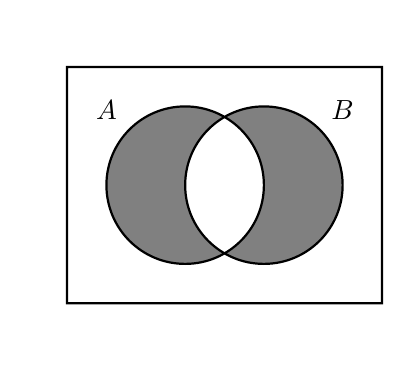
\begin{tikzpicture}[fill=gray]
% left hand
\scope
\clip (-2,-2) rectangle (2,2)
      (1,0) circle (1);
\fill (0,0) circle (1);
\endscope
% right hand
\scope
\clip (-2,-2) rectangle (2,2)
      (0,0) circle (1);
\fill (1,0) circle (1);
\endscope
% outline
\draw[thick] (0,0) circle (1) (-1,.7)  node [text=black,above] {$A$}
      (1,0) circle (1) (2,.7)  node [text=black,above] {$B$}
      (-1.5,-1.5) rectangle (2.5,1.5);
\end{tikzpicture}
\end{center}

  \begin{answer}
    For example, $A \cup B \cap \bar{(A \cap B)}$.  Note that $\bar{A \cap B}$ would almost work, but also contain the area outside of both circles.
  \end{answer}

  

\question Find the cardinalities:
\begin{parts}
  \part Find $|A|$ when $A = \{4,5,6,\ldots,37\}$
  \part Find $|A|$ when $A = \{x \in \Z \st -2 \le x \le 100\}$
  \part Find $|A \cap B|$ when $A = \{x \in \N \st x \le 20\}$ and $B = \{x \in \N \st x \mbox{ is prime}\}$
\end{parts}

  \begin{answer}
      \begin{parts}
	  \part 34.
	  \part 103.
	  \part 8.
      \end{parts}
  \end{answer}


  
  
\question Let $A = \{a, b, c\}$.  Find $\pow(A)$.

  \begin{answer}
    $\pow(A) = \{\emptyset, \{a\}, \{b\}, \{c\}, \{a,b\}, \{a,c\}, \{b,c\}, \{a,b,c\}\}$.
  \end{answer}

  
  

\question Let $A = \{1,2,\ldots, 10\}$.  How many subsets of $A$ contain exactly one element (i.e., how many {\em singleton} subsets are there).  How many {\em doubleton} (containing exactly two elements) are there?

  \begin{answer}
      There are 10 singletons.  There are 45 doubletons (because $45 = 9+8+7+\cdots+2+1$).
  \end{answer}


  
  
\question Let $A = \{1,2,3,4,5,6\}$.  Find all sets $B \in \pow(A)$ which have the property $\{2,3,5\} \subseteq B$.

  \begin{answer}
      $\{2,3,5\}, \{1,2,3,5\}, \{2,3,4,5\}, \{2,3,5,6\}, \{1,2,3,4,5\}, \{1,2,3,5,6\}, \{2,3,4,5,6\}$, and $\{1,2,3,4,5,6\}$.
  \end{answer}


  
\question Find an example of sets $A$ and $B$ such that $|A| = 4$, $|B| = 5$ and $|A \cup B| = 9$.  

  \begin{answer}
   For example $A = \{1,2,3,4\}$ and $B = \{5,6,7,8,9\}$.
  \end{answer}

  
  

\question Find an example of sets $A$ and $B$ such that $|A| = 3$, $|B| = 4$ and $|A \cup B| = 5$.

  \begin{answer}
    For example, $A = \{1,2,3\}$ and $B = \{2,3,4,5\}$.
  \end{answer}



\question In a regular deck of playing cards there are 26 red cards and 12 face cards.  Explain in terms of sets why there are only 32 cards which are either red or a face card.

  \begin{answer}
      If $R$ is the set of red cards and $F$ is the set of face cards, we want to find $|R \cup F|$.  This is not simply $|R| + |F|$ because there are 6 cards which are both red and a face card; $|R \cap F| = 6$.  We find $|R \cup F| = 32$.
  \end{answer}


  
% \question A group of college students were asked about their TV watching habits.  Of those surveyed, 28 students watch {\em House}, 19 watch {\em Castle} and 24 watch re-runs of {\em 24}.  Additionally, 16 watch {\em House} and {\em Castle}, 14 watch {\em House} and {\em 24} and 10 watch {\em Castle} and {\em 24}.  There are 8 students who watch all three shows.  How many students surveyed watched at least one of the shows?
% 
%   \begin{answer}
%     39.
%   \end{answer}
% 
% 
% 
% \question Find $|(A \cup C)\cap \bar B|$ provided $|A| = 50$, $|B| = 45$, $|C| = 40$, $|A\cap B| = 20$, $|A \cap C| = 15$, $|B \cap C| = 23$ and $|A \cap B \cap C| = 12$.
% 
%     \begin{answer}
%       $|(A \cup C)\cap \bar B| = 44$
%     \end{answer}
% 
% 
% 
% \question Using the same data as the previous question, describe a set with cardinality 26.
% 
%     \begin{answer}
% 	One possibility: $(A \cup B) \cap C$.
%     \end{answer}



  

% \question Consider the statement ``for all integers $a$ and $b$, if $a + b$ is even, then $a$ and $b$ are even''
% \begin{parts}
%  \part Write the contrapositive of the statement
%  \part Write the converse of the statement
%  \part Write the negation of the statement.
%  \part Is the original statement true or false?  Prove your answer.
%  \part Is the contrapositive of the original statement true or false?  Prove your answer.
%  \part Is the converse of the original statement true or false?  Prove your answer.
%  \part Is the negation of the original statement true or false?  Prove your answer.
% \end{parts}
% 
%   \begin{answer}
%     \begin{parts}
% 	\part For all integers $a$ and $b$, if $a$ or $b$ are not even, then $a+b$ is not even.
% 	\part For all integers $a$ and $b$, if $a$ and $b$ are even, then $a+b$ is even.
% 	\part There are numbers $a$ and $b$ such that $a+b$ is even but $a$ and $b$ are not both even.
% 	\part False.  For example, $a = 3$ and $b = 5$.  $a+b = 8$, but neither $a$ nor $b$ are even.
% 	\part False, since it is equivalent to the original statement.
% 	\part True.  Let $a$ and $b$ be integers.  Assume both are even.  Then $a = 2k$ and $b = 2j$ for some integers $k$ and $j$.  But then $a+b = 2k + 2j = 2(k+j)$ which is even.
% 	\part True, since the statement is false.
%       \end{parts}
%   \end{answer}
% 
% 
%   
%   
% \question Prove that $\sqrt 3$ is irrational.
% 
%   \begin{answer}
%     \begin{proof}
%      Suppose $\sqrt{3}$ were rational.  Then $\sqrt{3} = \frac{a}{b}$ for some integers $a$ and $b \ne 0$.  Without loss of generality, assume $\frac{a}{b}$ is reduced.  Now
% \[3 = \frac{a^2}{b^2}\]
% \[b^2 3 = a^2\]
% So $a^2$ is a multiple of 3.  This can only happen if $a$ is a multiple of 3, so $a = 3k$ for some integer $k$.  Then we have
% \[b^2 3 = 9k^2\]
% \[b^2 = 3k^2\]
% So $b^2$ is a multiple of 3, making $b$ a multiple of 3 as well.  But this contradicts our assumption that $\frac{a}{b}$ is in lowest terms.
%     \end{proof}
%   \end{answer}

 
 
 
  
% \question Translate into symbols.  Use $E(x)$ for ``$x$ is even'' and $O(x)$ for ``$x$ is odd.''
%  \begin{parts}
%   \part No number is both even and odd.
% \part One more than any even number is an odd number.
% \part There is prime number that is even.
% \part Between any two numbers there is a third number.
% \part There is no number between a number and one more than that number.
%  \end{parts}
% 
%   \begin{answer}
%      \begin{parts}
% 	\part $\neg \exists x (E(x) \wedge O(x))$
% 	\part $\forall x (E(x) \imp O(x+1))$
% 	\part $\exists x(P(x) \wedge E(x))$ (where $P(x)$ means ``$x$ is prime'')
% 	\part $\forall x \forall y \exists z(x < z < y \vee y < z < x)$
% 	\part $\forall x \neg \exists y (x < y < x+1)$
%     \end{parts}
%   \end{answer}
% 
%   
%  
%  
% \question Translate into English:
% \begin{parts}
%  \part $\forall x (E(x) \imp E(x +2))$
% \part $\forall x \exists y (\sin(x) = y)$
% \part $\forall y \exists x (\sin(x) = y)$
% \part $\forall x \forall y (x^3 = y^3 \imp x = y)$
% \end{parts}
% 
%   \begin{answer}
%     \begin{parts}
% 	\part Any even number plus 2 is an even number.
% 	\part For any $x$ there is a $y$ such that $\sin(x) = y$.  In other words, every number $x$ is in the domain of sine. 
% 	\part For every $y$ there is an $x$ such that $\sin(x) = y$.  In other words, every number $y$ is in the range of sine (which is false).
% 	\part For any numbers, if the cubes of two numbers are equal, then the numbers are equal.
%       \end{parts}
%   \end{answer}
% 
%   
%   
% 
% \question Simplify the statements (so negation appears only directly next to predicates).
% \begin{parts}
%   \part $\neg \exists x \forall y (\neg O(x) \vee E(y))$
%   \part $\neg \forall x \neg \forall y \neg(x < y \wedge \exists z (x < z \vee y < z))$
%   \part There is a number $n$ for which no other number is either less $n$ than or equal to $n$.
%   \part It is false that for every number $n$ there are two other numbers which $n$ is between.
% \end{parts}
% 
%   \begin{answer}
%     \begin{parts}
% 	\part $\forall x \exists y (O(x) \wedge \neg E(y))$
% 	\part $\exists x \forall y (x \ge y \vee \forall z (x \ge z \wedge y \ge z))$
% 	\part There is a number $n$ for which every other number is strictly greater than $n$.
% 	\part There is a number $n$ which is not between any other two numbers.
%       \end{parts}
%   \end{answer}
% 
%   
% 
% 
% \question Consider the statement ``for all integers $a$ and $b$, if $a + b$ is even, then $a$ and $b$ are even''
% \begin{parts}
%  \part Write the contrapositive of the statement
%  \part Write the converse of the statement
%  \part Write the negation of the statement.
%  \part Is the original statement true or false?  Prove your answer.
%  \part Is the contrapositive of the original statement true or false?  Prove your answer.
%  \part Is the converse of the original statement true or false?  Prove your answer.
%  \part Is the negation of the original statement true or false?  Prove your answer.
% \end{parts}
% 
%   \begin{answer}
%     \begin{parts}
% 	\part For all integers $a$ and $b$, if $a$ or $b$ are not even, then $a+b$ is not even.
% 	\part For all integers $a$ and $b$, if $a$ and $b$ are even, then $a+b$ is even.
% 	\part There are numbers $a$ and $b$ such that $a+b$ is even but $a$ and $b$ are not both even.
% 	\part False.  For example, $a = 3$ and $b = 5$.  $a+b = 8$, but neither $a$ nor $b$ are even.
% 	\part False, since it is equivalent to the original statement.
% 	\part True.  Let $a$ and $b$ be integers.  Assume both are even.  Then $a = 2k$ and $b = 2j$ for some integers $k$ and $j$.  But then $a+b = 2k + 2j = 2(k+j)$ which is even.
% 	\part True, since the statement is false.
%       \end{parts}
%   \end{answer}
% 
% 
%   
%   
% \question Prove that $\sqrt 3$ is irrational.
% 
%   \begin{answer}
%     \begin{proof}
%      Suppose $\sqrt{3}$ were rational.  Then $\sqrt{3} = \frac{a}{b}$ for some integers $a$ and $b \ne 0$.  Without loss of generality, assume $\frac{a}{b}$ is reduced.  Now
% \[3 = \frac{a^2}{b^2}\]
% \[b^2 3 = a^2\]
% So $a^2$ is a multiple of 3.  This can only happen if $a$ is a multiple of 3, so $a = 3k$ for some integer $k$.  Then we have
% \[b^2 3 = 9k^2\]
% \[b^2 = 3k^2\]
% So $b^2$ is a multiple of 3, making $b$ a multiple of 3 as well.  But this contradicts our assumption that $\frac{a}{b}$ is in lowest terms.
%     \end{proof}
%   \end{answer}
% 
%  
 
 
\end{questions}




%%
\begin{questions}

  
\question Translate into symbols.  Use $E(x)$ for ``$x$ is even'' and $O(x)$ for ``$x$ is odd.''
 \begin{parts}
  \part No number is both even and odd.
\part One more than any even number is an odd number.
\part There is prime number that is even.
\part Between any two numbers there is a third number.
\part There is no number between a number and one more than that number.
 \end{parts}

  \begin{answer}
     \begin{parts}
	\part $\neg \exists x (E(x) \wedge O(x))$
	\part $\forall x (E(x) \imp O(x+1))$
	\part $\exists x(P(x) \wedge E(x))$ (where $P(x)$ means ``$x$ is prime'')
	\part $\forall x \forall y \exists z(x < z < y \vee y < z < x)$
	\part $\forall x \neg \exists y (x < y < x+1)$
    \end{parts}
  \end{answer}

  
 
 
\question Translate into English:
\begin{parts}
 \part $\forall x (E(x) \imp E(x +2))$
\part $\forall x \exists y (\sin(x) = y)$
\part $\forall y \exists x (\sin(x) = y)$
\part $\forall x \forall y (x^3 = y^3 \imp x = y)$
\end{parts}

  \begin{answer}
    \begin{parts}
	\part Any even number plus 2 is an even number.
	\part For any $x$ there is a $y$ such that $\sin(x) = y$.  In other words, every number $x$ is in the domain of sine. 
	\part For every $y$ there is an $x$ such that $\sin(x) = y$.  In other words, every number $y$ is in the range of sine (which is false).
	\part For any numbers, if the cubes of two numbers are equal, then the numbers are equal.
      \end{parts}
  \end{answer}

  
  

\question Simplify the statements (so negation appears only directly next to predicates).
\begin{parts}
  \part $\neg \exists x \forall y (\neg O(x) \vee E(y))$
  \part $\neg \forall x \neg \forall y \neg(x < y \wedge \exists z (x < z \vee y < z))$
  \part There is a number $n$ for which no other number is either less $n$ than or equal to $n$.
  \part It is false that for every number $n$ there are two other numbers which $n$ is between.
\end{parts}

  \begin{answer}
    \begin{parts}
	\part $\forall x \exists y (O(x) \wedge \neg E(y))$
	\part $\exists x \forall y (x \ge y \vee \forall z (x \ge z \wedge y \ge z))$
	\part There is a number $n$ for which every other number is strictly greater than $n$.
	\part There is a number $n$ which is not between any other two numbers.
      \end{parts}
  \end{answer}

  
\question Let $A = \{1,2,3,4,5\}$, $B = \{3,4,5,6,7\}$ and $C = \{2,3,5\}$.
\begin{parts}
 \part Find $A \cap B$.
 \part Find $A \cup B$.
 \part Find $A \setminus B$.
 \part Is $C \subseteq A$?
 \part Is $C \subseteq B$?
\end{parts}

  \begin{answer}
    \begin{parts}
	\part $A \cap B = \{3,4,5\}$.  %Find $A \cap B$.
	\part $A \cup B = \{1,2,3,4,5,6,7\}$. %Find $A \cup B$.
	\part $A \setminus B = \{1,2\}$. %Find $A \setminus B$.
	\part Yes.  %Is $C \subseteq A$?
	\part No. %Is $C \subseteq B$?
    \end{parts}
  \end{answer}

  

\question Let $A = \{x \in \N \st 3 \le x \le 13\}$, $B = \{x \in \N \st x \mbox{ is even}\}$, and $C = \{x \in \N \st x \mbox{ is odd}\}$.
\begin{parts}
  \part Find $A \cap B$.
  \part Find $A \cup B$.
  \part Find $B \cap C$.
  \part Find $B \cup C$.
\end{parts}

  \begin{answer}
    \begin{parts}
  %Find $A \cap B$
	\part $A \cap B = \{4,6,8,10,12\}$
  % Find $A \cup B$.
	\part $A \cup B = \{x \in \N \st (3 \le x \le 13) \vee x \mbox{ is even}\}.$ (the set of all natural numbers which are either even or between 3 and 13 inclusive).
  %Find $B \cap C$.
	\part $B \cap C = \emptyset$.
  %Find $B \cup C$.
	\part $B \cup C = \N$.
      \end{parts}
  \end{answer}



\question Find an example of sets $A$ and $B$ such that $A\cap B = \{3, 5\}$ and $A \cup B = \{2, 3, 5, 7, 8\}$.

  \begin{answer}
    For example, $A = \{2,3,5,7,8\}$ and $B = \{3,5\}$.
  \end{answer}



\question Find an example of sets $A$ and $B$ such that $A \subseteq B$ and $A \in B$.

  \begin{answer}
    Let $A = \{1,2,3\}$ and $B = \{1,2,3,4,5,\{1,2,3\}\}$
  \end{answer}

  

\question Recall $\Z = \{\ldots,-2,-1,0, 1,2,\ldots\}$ (the integers).  Let $\Z^+$ be the positive integers.  Let $2\Z$ be the even integers, $3\Z$ be the multiples of 3, and so on.
\begin{parts}
  \part Is $\Z^+ \subseteq 2\Z$?  
  \part Is $2\Z \subseteq \Z^+$?  
  \part Find $2\Z \cap 3\Z$.  Describe the set in words, and also in symbols (using a $\st$ symbol).
  \part Express $\{x \in \Z \st \exists y\in \Z (x = 2y \vee x = 3y)\}$ as a union or intersection of two sets above.
\end{parts}

  \begin{answer}
    \begin{parts}
	\part No.
	\part No.
	\part $2\Z \cap 3\Z$ is the set of all integers which are multiples of both 2 and 3 (so multiples of 6).  Therefore $2\Z \cap 3\Z = \{x \in \Z \st \exists y\in \Z(x = 6y)\}$.
	\part $2\Z \cup 3\Z$.
 \end{parts}
  \end{answer}



\question Let $A_2$ be the set of all multiples of 2 except for $2$.  Let $A_3$ be the set of all multiples of 3 except for 3.  And so on, so that $A_n$ is the set of all multiple of $n$ except for $n$, for any $n \ge 2$.  Describe (in words) the set $\bar{A_2 \cup A_3 \cup A_4 \cup \cdots}$

  \begin{answer}
    The set of primes.
  \end{answer}




\question Draw a Venn diagram to represent each of the following:
\begin{parts}
 \part $A \cup \bar B$
 \part $\bar{(A \cup B)}$
 \part $A \cap (B \cup C)$
 \part $(A \cap B) \cup C$
 \part $\bar A \cap B \cap \bar C$
 \part $(A \cup B) \setminus C$
\end{parts}

  \begin{answer}	  
%  \begin{multicols}{3}
      \begin{parts}
	  \def\circleA{(-.5,0) circle (1)}
	  \def\circleAlabel{(-1.5,.6) node[above]{$A$}}
	  \def\circleB{(.5,0) circle (1)}
	  \def\circleBlabel{(1.5,.6) node[above]{$B$}}
	  \def\circleC{(0,-1) circle (1)}
	  \def\circleClabel{(.5,-2) node[right]{$C$}}
	  \def\twosetbox{(-2,-1.5) rectangle (2,1.5)}
	  \def\threesetbox{(-2,-2.5) rectangle (2,1.5)}
	  

	  
	    \part  $A \cup \bar B$:
	    
	    \begin{tikzpicture}[fill=gray!50]
	  %Fill A:
	  \fill \circleA;
	  %Fill \bar B:
	    \begin{scope}
	    \clip \circleB \twosetbox; %This defines the scope to everything in the twosetbox which is not in circleB.
	    \fill \twosetbox;
	    \end{scope}
	    \draw[thick] \circleA \circleAlabel \circleB \circleBlabel \twosetbox;
	  \end{tikzpicture}


	  %   
	  \part $\bar{(A \cup B)}$:

	  \begin{tikzpicture}[fill=gray!50]
	    \fill \twosetbox;
	    \fill[white] \circleA \circleB;
	    \draw[thick] \circleA \circleAlabel \circleB \circleBlabel \twosetbox;
	  \end{tikzpicture}

%	  \columnbreak

	  %   
	  \part $A \cap (B \cup C)$:

	  \begin{tikzpicture}[fill=gray!50]
	  \begin{scope}
	    \clip \circleA;
	    \fill \circleB \circleC;
	  \end{scope}
	  \draw[thick] \circleA \circleAlabel \circleB \circleBlabel \circleC \circleClabel \threesetbox;
	  \end{tikzpicture}

	  %  
	  \part $(A \cap B) \cup C$:

	  \begin{tikzpicture}[fill=gray!50]
	  \begin{scope}
	    \clip \circleA;
	    \fill \circleB;
	  \end{scope}
	  \fill \circleC;
	  \draw[thick] \circleA \circleAlabel \circleB \circleBlabel \circleC \circleClabel \threesetbox;
	  \end{tikzpicture}

	 
%	  \columnbreak
	  %   
	  \part $\bar A \cap B \cap \bar C$:

	  \begin{tikzpicture}[fill=gray!50]
	  \fill \circleB;
	  \begin{scope}
	    \clip \circleB;
	    \fill[white] \circleA \circleC;
	  \end{scope}

	  \draw[thick] \circleA \circleAlabel \circleB \circleBlabel \circleC \circleClabel \threesetbox;
	  \end{tikzpicture}

	  %   
	  \part $(A \cup B) \setminus C$:

	  \begin{tikzpicture}[fill=gray!50]
	  \fill \circleA;
	  \fill \circleB;
	  \fill[white] \circleC;
	  \draw[thick] \circleA \circleAlabel \circleB \circleBlabel \circleC \circleClabel \threesetbox;
	  \end{tikzpicture}

	  \end{parts}	 
%	   \end{multicols}
  \end{answer}




\question Describe a set in terms of $A$ and $B$ which has the following Venn diagram:

\begin{center}
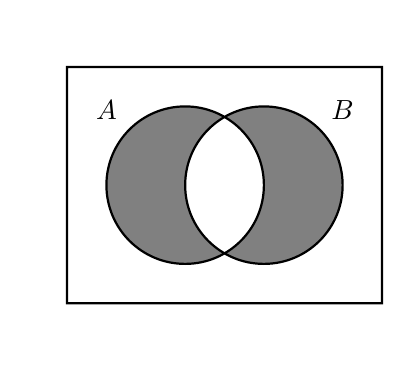
\begin{tikzpicture}[fill=gray]
% left hand
\scope
\clip (-2,-2) rectangle (2,2)
      (1,0) circle (1);
\fill (0,0) circle (1);
\endscope
% right hand
\scope
\clip (-2,-2) rectangle (2,2)
      (0,0) circle (1);
\fill (1,0) circle (1);
\endscope
% outline
\draw[thick] (0,0) circle (1) (-1,.7)  node [text=black,above] {$A$}
      (1,0) circle (1) (2,.7)  node [text=black,above] {$B$}
      (-1.5,-1.5) rectangle (2.5,1.5);
\end{tikzpicture}
\end{center}

  \begin{answer}
    For example, $A \cup B \cap \bar{(A \cap B)}$.  Note that $\bar{A \cap B}$ would almost work, but also contain the area outside of both circles.
  \end{answer}

  

\question Find the cardinalities:
\begin{parts}
  \part Find $|A|$ when $A = \{4,5,6,\ldots,37\}$
  \part Find $|A|$ when $A = \{x \in \Z \st -2 \le x \le 100\}$
  \part Find $|A \cap B|$ when $A = \{x \in \N \st x \le 20\}$ and $B = \{x \in \N \st x \mbox{ is prime}\}$
\end{parts}

  \begin{answer}
      \begin{parts}
	  \part 34.
	  \part 103.
	  \part 8.
      \end{parts}
  \end{answer}


  
  
\question Let $A = \{a, b, c\}$.  Find $\pow(A)$.

  \begin{answer}
    $\pow(A) = \{\emptyset, \{a\}, \{b\}, \{c\}, \{a,b\}, \{a,c\}, \{b,c\}, \{a,b,c\}\}$.
  \end{answer}

  
  

\question Let $A = \{1,2,\ldots, 10\}$.  How many subsets of $A$ contain exactly one element (i.e., how many {\em singleton} subsets are there).  How many {\em doubleton} (containing exactly two elements) are there?

  \begin{answer}
      There are 10 singletons.  There are 45 doubletons (because $45 = 9+8+7+\cdots+2+1$).
  \end{answer}


  
  
\question Let $A = \{1,2,3,4,5,6\}$.  Find all sets $B \in \pow(A)$ which have the property $\{2,3,5\} \subseteq B$.

  \begin{answer}
      $\{2,3,5\}, \{1,2,3,5\}, \{2,3,4,5\}, \{2,3,5,6\}, \{1,2,3,4,5\}, \{1,2,3,5,6\}, \{2,3,4,5,6\}$, and $\{1,2,3,4,5,6\}$.
  \end{answer}


  
\question Find an example of sets $A$ and $B$ such that $|A| = 4$, $|B| = 5$ and $|A \cup B| = 9$.  

  \begin{answer}
   For example $A = \{1,2,3,4\}$ and $B = \{5,6,7,8,9\}$.
  \end{answer}

  
  

\question Find an example of sets $A$ and $B$ such that $|A| = 3$, $|B| = 4$ and $|A \cup B| = 5$.

  \begin{answer}
    For example, $A = \{1,2,3\}$ and $B = \{2,3,4,5\}$.
  \end{answer}



\question In a regular deck of playing cards there are 26 red cards and 12 face cards.  Explain in terms of sets why there are only 32 cards which are either red or a face card.

  \begin{answer}
      If $R$ is the set of red cards and $F$ is the set of face cards, we want to find $|R \cup F|$.  This is not simply $|R| + |F|$ because there are 6 cards which are both red and a face card; $|R \cap F| = 6$.  We find $|R \cup F| = 32$.
  \end{answer}


  
% \question A group of college students were asked about their TV watching habits.  Of those surveyed, 28 students watch {\em House}, 19 watch {\em Castle} and 24 watch re-runs of {\em 24}.  Additionally, 16 watch {\em House} and {\em Castle}, 14 watch {\em House} and {\em 24} and 10 watch {\em Castle} and {\em 24}.  There are 8 students who watch all three shows.  How many students surveyed watched at least one of the shows?
% 
%   \begin{answer}
%     39.
%   \end{answer}
% 
% 
% 
% \question Find $|(A \cup C)\cap \bar B|$ provided $|A| = 50$, $|B| = 45$, $|C| = 40$, $|A\cap B| = 20$, $|A \cap C| = 15$, $|B \cap C| = 23$ and $|A \cap B \cap C| = 12$.
% 
%     \begin{answer}
%       $|(A \cup C)\cap \bar B| = 44$
%     \end{answer}
% 
% 
% 
% \question Using the same data as the previous question, describe a set with cardinality 26.
% 
%     \begin{answer}
% 	One possibility: $(A \cup B) \cap C$.
%     \end{answer}



  

% \question Consider the statement ``for all integers $a$ and $b$, if $a + b$ is even, then $a$ and $b$ are even''
% \begin{parts}
%  \part Write the contrapositive of the statement
%  \part Write the converse of the statement
%  \part Write the negation of the statement.
%  \part Is the original statement true or false?  Prove your answer.
%  \part Is the contrapositive of the original statement true or false?  Prove your answer.
%  \part Is the converse of the original statement true or false?  Prove your answer.
%  \part Is the negation of the original statement true or false?  Prove your answer.
% \end{parts}
% 
%   \begin{answer}
%     \begin{parts}
% 	\part For all integers $a$ and $b$, if $a$ or $b$ are not even, then $a+b$ is not even.
% 	\part For all integers $a$ and $b$, if $a$ and $b$ are even, then $a+b$ is even.
% 	\part There are numbers $a$ and $b$ such that $a+b$ is even but $a$ and $b$ are not both even.
% 	\part False.  For example, $a = 3$ and $b = 5$.  $a+b = 8$, but neither $a$ nor $b$ are even.
% 	\part False, since it is equivalent to the original statement.
% 	\part True.  Let $a$ and $b$ be integers.  Assume both are even.  Then $a = 2k$ and $b = 2j$ for some integers $k$ and $j$.  But then $a+b = 2k + 2j = 2(k+j)$ which is even.
% 	\part True, since the statement is false.
%       \end{parts}
%   \end{answer}
% 
% 
%   
%   
% \question Prove that $\sqrt 3$ is irrational.
% 
%   \begin{answer}
%     \begin{proof}
%      Suppose $\sqrt{3}$ were rational.  Then $\sqrt{3} = \frac{a}{b}$ for some integers $a$ and $b \ne 0$.  Without loss of generality, assume $\frac{a}{b}$ is reduced.  Now
% \[3 = \frac{a^2}{b^2}\]
% \[b^2 3 = a^2\]
% So $a^2$ is a multiple of 3.  This can only happen if $a$ is a multiple of 3, so $a = 3k$ for some integer $k$.  Then we have
% \[b^2 3 = 9k^2\]
% \[b^2 = 3k^2\]
% So $b^2$ is a multiple of 3, making $b$ a multiple of 3 as well.  But this contradicts our assumption that $\frac{a}{b}$ is in lowest terms.
%     \end{proof}
%   \end{answer}

 
 
 
\end{questions}






%%%\documentclass[12pt]{article}

\usepackage{discrete}

\def\thetitle{Functions} % will be put in the center header on the first page only.
\def\lefthead{Math 228 Notes} % will be put in the left header
\def\righthead{Functions} % will be put in the right header


\begin{document}

A function\index{function} is a rule that assigns each input exactly one output.  The set of all inputs for a function is called the \emph{domain}\index{domain}.  The set of all allowable outputs is called the \emph{codomain}\index{codomain}.  For example, a function might assign each natural number a natural number from 1 to 5.  In that case, the domain is the natural numbers and the codomain is the set of natural numbers from 1 to 5. Now it could be that this particular function we are thinking about assigns each even natural number to the number 2 and each odd natural number to the number 1.  In this case, not all of the codomain is actually used.  We would say that the set $\{1,2\}$ is the \emph{range}\index{range} of the function. These are the elements in the codomain (allowable outputs) which are actually outputs for some input. 

The key thing that makes a rule assigning inputs to outputs a \emph{function} is that there is \emph{only one} output for an input.  In other words, it is important that the rule be a good rule.  What output do we assign to the input 7?  There can only be one answer for any particular function. 

To specify the name of the function, as well as the domain and codomain, we write $f:X \to Y$.  The function is called $f$, the domain is the set $X$ and the codomain is the set $Y$.  This however does not describe the rule.  To do that, we say something like this:

\begin{quote}
  The function $f:X \to Y$ is defined by $f(x) = x^2 + 3$.
\end{quote}

This function takes an input $x$ and computes the output by squaring $x$ and then adding 3.  In this case, you better hope that $X$ is a set of numbers and $Y$ is a set of number which can be 3 more than squares of numbers from $X$.  It would not work for $Y$ to be negative numbers here. That would not be a valid function.

The description of the rule can vary greatly.  If $X$ is a finite set, we might just give a list of each output for each input.  You could also describe the function with a table or a graph or in words.

\begin{example}
  The following are all examples of functions:
  \begin{enumerate}
    \item $f:\Z \to \Z$ defined by $f(n) = 3n$.  The domain and codomain are both the set of integers.  However, the range is only the set of integer multiples of 3.
    \item $f: \{1,2,3\} \to \{a,b,c\}$ defined by $f(1) = c$, $f(2) = a$ and $f(3) = a$.  The domain is the set $\{1,2,3\}$, the codomain is the set $\{a,b,c\}$ and the range is the set $\{a,c\}$.  Note that $f(2)$ and $f(3)$ are the same element of codomain.  This is not a problem.  Each element in the domain still has only one output (although each output does not have a unique input).
    \item $f:\{1,2,3\} \to \{1,2,3\}$ defined as follows:
    \begin{center}
      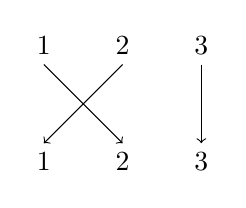
\begin{tikzpicture}
        \draw[->] (-1,1) node[above] {1} -- (0,0) node[below] {2};
        \draw[->] (0,1) node[above] {2} -- (-1,0) node[below] {1};
        \draw[->] (1,1) node[above] {3} -- (1,0) node[below] {3};
      \end{tikzpicture}

    \end{center}

  \end{enumerate}

\end{example}

The arrow diagram used to define the function above can be very helpful in visualizing functions.  We will often be working with functions on finite sets so this kind of picture is often more useful than a traditional graph of a function.  A graph of the function in example 3 above would look like this:

\begin{center}
  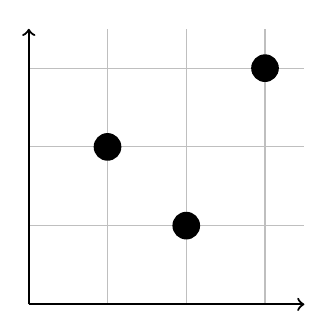
\begin{tikzpicture}
    %axis:
    \draw[thin, gray!50] (0,0) grid (3.5, 3.5);
    \draw[->, thick] (0,0) -- (0,3.5);
   \draw[->, thick] (0,0) -- (3.5,0);
   %points:
   \fill (1,2) circle (5pt) (2,1) circle (5pt) (3,3) circle (5pt);
  \end{tikzpicture}

\end{center}

It would be absolutely WRONG to connect the dots or try to fit them to some curve.  There are only three elements in the domain.  A curve suggests that the domain contains an entire interval of real numbers.  Remember, we are not in calculus any more!

It is important to know how to recognize a function from a rule which is not a function.  The arrow diagram can help.

\begin{example}
Which of the following diagrams represent a function.  Let $X = \{1,2,3,4\}$ and $Y = \{a,b,c,d\}$
  \begin{multicols}{3}
    \begin{center}
      $f:X \to Y$
      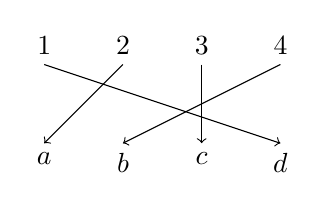
\begin{tikzpicture}
        \draw[->] (-1.5,1) node[above] {1} -- (1.5,0) node[below] {$d$};
        \draw[->] (-.5,1) node[above] {2} -- (-1.5,0) node[below] {$a$};
        \draw[->] (.5,1) node[above] {3} -- (.5, 0) node[below] {$c$};
        \draw[->] (1.5,1) node[above] {4} -- (-.5, 0) node[below] {$b$};
      \end{tikzpicture}
      \columnbreak
      
      $g:X \to Y$
	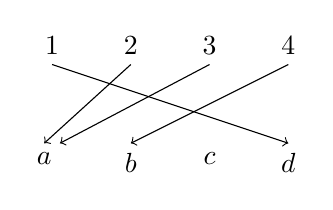
\begin{tikzpicture}
        \draw[->] (-1.5,1) node[above] {1} -- (1.5,0) node[below] {$d$};
        \draw[->] (-.5,1) node[above] {2} -- (-1.6,0) node[below] {$a$};
        \draw[->] (.5,1) node[above] {3} -- (-1.4, 0);
        \draw[->] (1.5,1) node[above] {4} -- (-.5, 0) node[below] {$b$};
        \draw (.5,0) node[below] {$c$};
      \end{tikzpicture}
      
      \columnbreak
      
      $h:X \to Y$
      	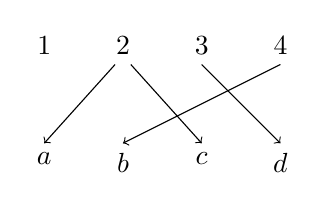
\begin{tikzpicture}
        \draw (-1.5,1) node[above] {1};
        \draw[->] (-.5,1) node[above] {2} (-.6,1) -- (-1.5,0) node[below] {$a$};
        \draw[->] (-.4,1) -- (.5,0);
        \draw[->] (.5,1) node[above] {3} -- (1.5, 0) node[below] {$d$};
        \draw[->] (1.5,1) node[above] {4} -- (-.5, 0) node[below] {$b$};
        \draw (.5,0) node[below] {$c$};
      \end{tikzpicture}
    \end{center}

  \end{multicols}
\begin{solution}
  $f$ is a function.  So is $g$.  There is no problem with an element of the codomain not being the output for any input, and there is no problem with $a$ from the codomain being the output of both 2 and 3 from the domain.  
  
  However, $h$ is \textbf{not} a function.  In fact, it fails for two reasons.  First, the element 1 from the domain has not been mapped to any element from the codomain.  Second, the element 2 from the domain has been mapped to more than one element from the codomain ($a$ and $c$).  Note that either one of these problems is enough to make a rule not a function.  Neither of these mappings are functions:
  \begin{center}
    \begin{multicols}{2}
      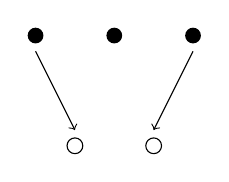
\begin{tikzpicture}
        \fill (-1, 1.2) circle (.1) (0,1.2) circle (.1) (1, 1.2) circle (.1);
        \draw[->] (-1, 1) -- (-.5,0);
        \draw[->] (1,1) -- (.5, 0);
        \draw (-.5, -0.2) circle (.1) (.5, -0.2) circle (.1);
      \end{tikzpicture}
       
       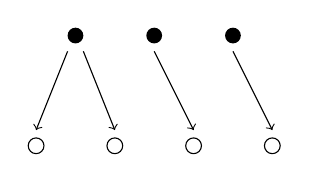
\begin{tikzpicture}
         \fill (-1, 1.2) circle (.1) (0,1.2) circle (.1) (1, 1.2) circle (.1);
         \draw[->] (-1.1, 1) -- (-1.5, 0);
         \draw[->] (-.9, 1) -- (-.5, 0);
         \draw[->] (0,1) -- (.5,0);
         \draw[->] (1,1) -- (1.5, 0);
         \draw (-.5, -0.2) circle (.1) (.5, -0.2) circle (.1) (-1.5, -0.2) circle (.1) (1.5, -0.2) circle (.1);
       \end{tikzpicture}

    \end{multicols}
  Not functions.
  \end{center}

\end{solution}

\end{example}

\subsection{Surjections, Injections, and Bijections}

We now turn to investigating special properties functions might or might not possess.  

In the examples above, you may have noticed that sometimes there are elements of the codomain which are not in the range.  When this sort of the thing \emph{does not} happen, (that is, when everything in the codomain is in the range) we say the function is \emph{onto}\index{onto|see {surjection}} or that the function maps the domain \emph{onto} the codomain.  This terminology should make sense: the function puts the domain (entirely) on top the codomain.  The fancy math term for an onto function is a \emph{surjection}\index{surjection}, and we say that an onto function is a \emph{surjective} function.

In pictures:

\begin{multicols}{2}
  \begin{center}
          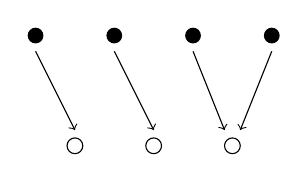
\begin{tikzpicture}
        \fill (-1.5, 1.2) circle (.1) (-.5,1.2) circle (.1) (.5, 1.2) circle (.1) (1.5,1.2) circle (.1);
        \draw[->] (-1.5, 1) -- (-1,0);
        \draw[->] (-.5,1) -- (0, 0);
        \draw[->] (.5, 1) -- (.9,0);
        \draw[->] (1.5,1) -- (1.1,0);
        \draw (-1, -0.2) circle (.1) (0, -0.2) circle (.1) (1, -0.2) circle (.1);
      \end{tikzpicture}
      
      Surjective
      
      \columnbreak
      
                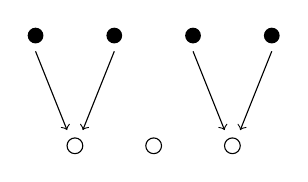
\begin{tikzpicture}
        \fill (-1.5, 1.2) circle (.1) (-.5,1.2) circle (.1) (.5, 1.2) circle (.1) (1.5,1.2) circle (.1);
        \draw[->] (-1.5, 1) -- (-1.1,0);
        \draw[->] (-.5,1) -- (-.9, 0);
        \draw[->] (.5, 1) -- (.9,0);
        \draw[->] (1.5,1) -- (1.1,0);
        \draw (-1, -0.2) circle (.1) (0, -0.2) circle (.1) (1, -0.2) circle (.1);
      \end{tikzpicture}
      
      Not surjective
  \end{center}

\end{multicols}

\begin{example}
  Which functions are surjective (i.e., onto)?
    \begin{enumerate}
    \item $f:\Z \to \Z$ defined by $f(n) = 3n$.  
    \item $g: \{1,2,3\} \to \{a,b,c\}$ defined by $g(1) = c$, $g(2) = a$ and $g(3) = a$.  
    \item $h:\{1,2,3\} \to \{1,2,3\}$ defined as follows:
    \begin{center}
      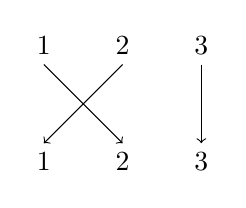
\begin{tikzpicture}
        \draw[->] (-1,1) node[above] {1} -- (0,0) node[below] {2};
        \draw[->] (0,1) node[above] {2} -- (-1,0) node[below] {1};
        \draw[->] (1,1) node[above] {3} -- (1,0) node[below] {3};
      \end{tikzpicture}
    \end{center}
  \end{enumerate}
  \begin{solution}
    \begin{enumerate}
      \item $f$ is not surjective.  There are elements in the codomain which are not in the range.  For example, no $n \in \Z$ gets mapped to the number 1 (the rule would say that $\frac{1}{3}$ would be sent to 1, but $\frac{1}{3}$ is not in the domain).  In fact, the range of the function is $3\Z$ (the integer multiples of 3), which is not equal to $\Z$.
      \item $g$ is not surjective.  There is no $x \in \{1,2,3\}$ (the domain) for which $g(x) = b$.  So $b$, which is in the codomain, is not in the range, so once again the function is not onto.
      \item $h$ is surjective.  Every element of the codomain is also in the range.  Nothing is missed.
    \end{enumerate}

  \end{solution}

\end{example}


To be a function, a map cannot assign a single element of the domain to two or more different elements of the codomain.  However, we have seen that the reverse is permissible.  That is, a function might assign the same element of the codomain to two or more different elements of the domain.  When this \emph{does not} occur (that is, when each element of the codomain is assigned to at most one element of the domain) then we say the function is \emph{one-to-one}\index{one-to-one|see {injection}}.  Again, this terminology makes sense: we are sending at most one element from the domain to one element from the codomain.  One input to one output. The fancy math term for a one-to-one function is an \emph{injection}\index{injection}.  We call one-to-one functions \emph{injective} functions.

In pictures:

\begin{multicols}{2}
  \begin{center}
          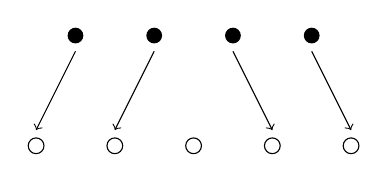
\begin{tikzpicture}
        \fill (-1.5, 1.2) circle (.1) (-.5,1.2) circle (.1) (.5, 1.2) circle (.1) (1.5,1.2) circle (.1);
        \draw[->] (-1.5, 1) -- (-2,0);
        \draw[->] (-.5,1) -- (-1, 0);
        \draw[->] (.5, 1) -- (1,0);
        \draw[->] (1.5,1) -- (2,0);
        \draw (-2, -0.2) circle (.1) (-1, -.2) circle (.1) (0, -0.2) circle (.1) (1, -0.2) circle (.1) (2, -0.2) circle (.1);
      \end{tikzpicture}
      
      Injective
      
      \columnbreak
      
                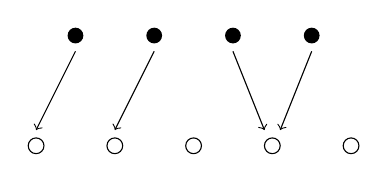
\begin{tikzpicture}
        \fill (-1.5, 1.2) circle (.1) (-.5,1.2) circle (.1) (.5, 1.2) circle (.1) (1.5,1.2) circle (.1);
        \draw[->] (-1.5, 1) -- (-2,0);
        \draw[->] (-.5,1) -- (-1, 0);
        \draw[->] (.5, 1) -- (.9,0);
        \draw[->] (1.5,1) -- (1.1,0);
        \draw (-2, -0.2) circle (.1) (-1, -.2) circle (.1) (0, -0.2) circle (.1) (1, -0.2) circle (.1) (2, -0.2) circle (.1);
      \end{tikzpicture}
      
      Not injective
  \end{center}

\end{multicols}


\begin{example}
  Which functions are injective (i.e., one-to-one)?
    \begin{enumerate}
    \item $f:\Z \to \Z$ defined by $f(n) = 3n$.  
    \item $g: \{1,2,3\} \to \{a,b,c\}$ defined by $g(1) = c$, $g(2) = a$ and $g(3) = a$.  
    \item $h:\{1,2,3\} \to \{1,2,3\}$ defined as follows:
    \begin{center}
      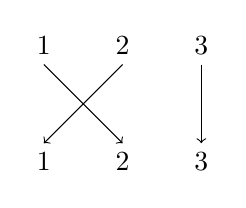
\begin{tikzpicture}
        \draw[->] (-1,1) node[above] {1} -- (0,0) node[below] {2};
        \draw[->] (0,1) node[above] {2} -- (-1,0) node[below] {1};
        \draw[->] (1,1) node[above] {3} -- (1,0) node[below] {3};
      \end{tikzpicture}
    \end{center}
  \end{enumerate}
  \begin{solution}
    \begin{enumerate}
      \item $f$ is injective.  Each element in the codomain is assigned to at \emph{most} one element from the domain.  If $x$ is a multiple of three, then only $x/3$ is mapped to $x$.  If $x$ is not a multiple of 3, then there is no input corresponding to the output $x$.
      \item $g$ is not injective.  Both inputs $2$ and $3$ are assigned the output $a$.
      \item $h$ is injective.  Each output is only an output once.
    \end{enumerate}

  \end{solution}

\end{example}



From the examples above, it should be clear that there are functions which are surjective, injective, both or neither.  In the case when a function is both one-to-one and onto (a injection and surjection) we say the function is a \emph{bijection}, or that the function is a \emph{bijective} function.  

\subsection{Inverse Image}

When discussing functions, we have notation for talking about an element of the domain (say $x$) and its corresponding element in the codomain (we write $f(x)$).  It would also be nice to start with some element of the codomain (say $y$) and talk about which element or elements (if any) from the domain get sent to it.  We could write ``those $x$ in the domain such that $f(x) = y$,'' but this is a lot of writing.  So here is some notation to make our lives easier.

Suppose $f:X \to Y$ is a function.  For $y \in Y$ (an element of the codomain), we write $f\inv(y)$ to represent the \emph{set} of all elements in the domain $X$ which get sent to $y$.  That is, $f\inv(y) = \{x \in X \st f(x) = y\}$.  We say that $f\inv(y)$ is the \emph{complete inverse image}\index{inverse image} of $y$ under $f$.

\vskip 1em
\noindent\textbf{WARNING: $f\inv(y)$ is not an inverse function!!!!  Inverse functions only exist for bijections, but $f\inv(y)$ is defined for any function $f$.  The point: $f\inv(y)$ is a \underline{set}, not an element of the domain.}
\vskip 1em

\begin{example}
 Consider the function $f:\{1,2,3,4,5,6\} \to \{a,b,c,d\}$ given by $f(1) = a$, $f(2) = a$, $f(3) = b$, $f(4) = c$, $f(5) = c$ and $f(6) = c$.  Find the complete inverse image of each element in the codomain.
 \begin{solution}
  Remember, we are looking for sets.
  \[f\inv(a) = \{1,2\}\]
  \[f\inv(b) = \{3\}\]
  \[f\inv(c) = \{4,5,6\}\]
  \[f\inv(d) = \emptyset.\]
 \end{solution}
\end{example}

\begin{example} Consider the function $g:\Z \to \Z$ defined by $g(n) = n^2 + 1$.  Find $g\inv(1)$, $g\inv(2)$, $g\inv(3)$ and $g\inv(10)$.
 \begin{solution}
  To find $g\inv(1)$, we need to find all integers $n$ such that $n^2 + 1 = 1$.  Clearly only 0 works, so $g\inv(1) = \{0\}$ (note that even though there is only one element, we still write it as a set with one element in it).  
  
  To find $g\inv(2)$, we need to find all $n$ such that $n^2 + 1 = 2$.  We see $g\inv(2) = \{-1,1\}$.  
  
  If $n^2 + 1 = 3$, then we are looking for an $n$ such that $n^2 = 2$.  There are no such integers so $g\inv(3) = \emptyset$. 
  
  Finally, $g\inv(10) = \{-3, 3\}$ because $g(-3) = 10$ and $g(3) = 10$.
 \end{solution}

\end{example}

Since $f\inv(y)$ is a set, it makes sense to ask for $|f\inv(y)|$, the number of elements in the domain which map to $y$.

\begin{example}
 Find a function $f:\{1,2,3,4,5\} \to \N$ such that $|f\inv(7)| = 5$.  
 \begin{solution}
 There is only one such function.  We need five elements of the domain to map to the number $7 \in \N$.  Since there are only five elements in the domain, all of them must map to 7.  So $f(1) = 7$, $f(2) = 7$, $f(3) = 7$, $f(4) = 7$ and $f(5) = 7$.
 \end{solution}
\end{example}





\begin{defbox}{Function Definitions}
\begin{itemize}
  \item A \emph{function} is a rule that assigns each element of a set, called the \emph{domain}, to exactly one element of a second set, called the \emph{codomain}.
  \item Notation: $f:X \to Y$ is our way of saying that the function is called $f$, the domain is the set $X$ and the codomain is the set $Y$.
  \item $f(x) = y$ means the element $x$ of the domain (input) is assigned to the element $y$ of the codomain.  We say $y$ is an output.  Alternatively, we call $y$ the \emph{image of $x$ under $f$}.
  \item The \emph{range} is a subset of the codomain.  It is the set of all elements which are assigned to at least one element of the domain by the function.  That is, the range is the set of all outputs.
  \item A function is \emph{injective} (an \emph{injection} or \emph{one-to-one}) if every element of the codomain is the output for \textbf{at most} one element from the domain.
  \item A function is \emph{surjective} (a \emph{surjection} or \emph{onto}) if every element of the codomain is the output of \textbf{at least} one element of the domain.
  \item A \emph{bijection} is a function which is both an injection and surjection.  In other words, if every element of the codomain is the output of \textbf{exactly one} element of the domain.
  \item The \emph{complete inverse image} of an element in the codomain, written $f\inv(y)$ is the \textbf{set} of all element in the domain which are assigned to $y$ by the function.  
\end{itemize}

\end{defbox}



\end{document}

\setcounter{chapter}{1}
\chapter[Graph Theory]{Introduction to Graph Theory}

\documentclass[12pt]{article}

\usepackage{../discrete}

\usetikzlibrary{shapes}

\usepackage{pgf}

\heading{Math 228}{}{Graph Theory Notes}



\begin{document}
%\section{Introduction to Graphs}

Graph Theory is a relatively new area of mathematics, first studied by the super famous mathematician Leonhard Euler in 1735.  Since then it has blossomed in to a powerful tool used in nearly every branch of science and is currently an active area of mathematics research.  We will begin our study with the problem that started it all: The Seven Bridges of K\"onigsberg.

\begin{quote} In the time of Euler, in the town of K\"onigsberg in Prussia, there was a river containing two islands.  The islands were connected to the banks of the river by seven bridges (as seen below).  The bridges were very beautiful, and on their days off, townspeople would spend time walking over the bridges.  As time passed, a question arose: was it possible to plan a walk so that you cross each bridge once and only once?  Euler was able to answer this question.  Are you?
  \end{quote}
\centerline{\includegraphics[width=5in]{images/7bridgescolor.png}}

Try finding a path which uses each bridge exactly once.  

Here is another problem:  below is a drawing of four dots connected by some lines.  Is it possible to trace over each line once and only once (without lifting up your pencil)?  You must start and end on one of the dots.

\centerline{\begin{tikzpicture}[scale=1.5, yscale=.5]
 \draw[thick] (-1,-2) \v to [out=120, in=240] (-1,0) \v to [out=120, in=240] (-1,2) \v to [out=300, in=60] (-1,0) to [out=300, in=60] (-1,-2);
  \draw[thick] (1,0) \v -- (-1,2) (-1,0) -- (1,0) -- (-1,-2);
  \end{tikzpicture}}

There is an obvious connection between these two problems - any path through the dot and line drawing corresponds exactly to to path over the bridges of K\"onigsberg.  


Pictures like the dot and line drawing are called {\em graphs}.  Graphs are made up of a collection of dots (called {\em vertices}) and lines connecting those dots (called {\em edges}).  The nice thing about looking at graphs instead of pictures of rivers, islands and bridges is that we now have a mathematical object to study.  A {\em set} of vertices and a set of edges (in fact, we can take the set of edges to be a set of ordered pairs from the set of vertices).  We have distilled the ``important'' parts of the bridge picture for the purposes of the problem - it does not matter how big the islands are, what the bridges are made out of, if the river contains alligators, etc.  All that matters is which land masses are connected to which other land masses, and how many times.  This was the great insight that Euler had.

We will return to the question of finding paths through graphs later.  But first, here are a few other situations you can represent with graphs.

\begin{example}
  Al, Bob, Cam, Dan, and Euclid are all members of the social networking website {\em Facebook}.  The site allows members to be ``friends'' with each other.  It turns out that Al and Cam are friends, as are Bob and Dan.  Euclid is friends with everyone.  Represent this situation with a graph.
  \begin{solution}
    Each person will be represented by a vertex and each friendship will be represented by an edge - that is, there will be an edge between two vertices if and only if the people represented by those vertices are friends.  We get the following graph:
    
    \begin{center}
      \begin{tikzpicture}
        \draw[thick] (-1, 0) \vl{C} -- (0,1) \vb{E} -- (-1,2) \vl{A} -- (-1,0)(1,0) \vr{D} -- (0,1)  -- (1,2) \vr{B} -- (1,0);
      \end{tikzpicture}
    \end{center}
  \end{solution}

\end{example}


\begin{example}
  Each of three houses must be connected to each of three utilities.  Is it possible to do this without any of the utility lines crossing?
  \begin{solution}
    We will answer this question later.  For now, notice how we would ask this question in the context of graph theory.  We are really asking whether it is possible to redraw the graph below without any edges crossing (except at vertices).
    
    \begin{center}
      \begin{tikzpicture}[yscale=1.2]
        \draw[thick] (-1,1) \v -- (-1,0)\v  -- (0,1) \v -- (0,0) \v -- (1,1) \v -- (1,0) \v -- (0,1) -- (-1,0) -- (1,1) (1,0) -- (-1,1) -- (0,0);
      \end{tikzpicture}
    \end{center}

  \end{solution}

\end{example}

\section{Basics}

While we almost always think of graphs as pictures, these are really just visual representations of mathematical objects.  In fact, all a graph is is a set of vertices some pairs of which are ``related'' by an edge.  For example, we can describe one graph like this: the vertices are the letters $\{a,b,c,d\}$ and the edges are the pairs $\{(a,b), (a,c), (b,c), (b,d), (c,d)\}$.  In other words, we have four vertices, $a$, $b$, $c$, and $d$, and $a$ is connected (by an edge) to $b$ and $c$, $b$ is connected to both $c$ and $d$, and $c$ is also connected to $d$.  One way to draw this graph is this:
\begin{center}
  \begin{tikzpicture}
    \draw[thick] (-1,1) \vl{$a$} -- (1,1) \vr{$b$} (-1,1) -- (-1,-1) \vl{$c$} -- (1,-1) \vr{$d$} -- (1,1) -- (-1,-1);
  \end{tikzpicture}
\end{center}

However we could also have drawn the graph differently.  For example either of these:

\begin{center}
  \begin{tikzpicture}
    \draw[thick] (-1,1) \vl{$a$} -- (1,-1) \vr{$b$} (-1,1) -- (-1,-1) \vl{$c$} -- (1,1) \vr{$d$} -- (1,-1) -- (-1,-1);
  \end{tikzpicture}
  \hspace{1in}
    \begin{tikzpicture}
    \draw[thick] (-1.5,0) \vb{$a$} -- (-.5,0) \vb{$b$} (-1.5,0) .. controls (-.5,1) .. (.5,0) \vb{$c$} -- (1.5,0) \vb{$d$} .. controls (.5,1) .. (-.5,0) -- (.5,0);
  \end{tikzpicture}
\end{center}

Viewed as pictures, the graphs above are the same whether or not the vertices are labeled as they are, or at all.  In fact, two graphs are equal precisely when there is a way to label the vertices so that all the pairs of vertices which have edges in one graph also have edges in the other graph, and {\it vice versa}.  Two vertices which are connected by an edge are called {\em adjacent}.

The graph above is also particularly nice in that no pair of vertices is connected more than once, and no vertex is connected to itself.  The technical name for graphs like this (no double edges or single edge loops) is called {\em simple}.  The graph is also {\em connected} - you can get from any vertex to any other vertex by following some path of edges ($a$ and $d$ are connected by a path two edges long).  A graph that is not connected can be thought of as two separate graphs drawn close together. Unless otherwise stated, we will assume all graphs are connected.  However, our graphs might or might not be simple (the graph for the K\"onigsberg bridge problem is {\em not} simple).

The graph above does not have an edge between $a$ and $d$.  Thus it is possible to add an edge to the graph (and keep it simple).  If we add all possible edges (keeping the graph simple), then the resulting graph is said to be {\em complete}.  That is, a graph is complete if every pair of vertices is connected by an edge.  Since a graph is determined completely by which vertices are adjacent to which other vertices, there is only one complete graph with a given number of vertices.  We give these a special name: $K_n$ is the complete graph on $n$ vertices.

Each vertex in $K_n$ is adjacent to $n-1$ other vertices.  We call the number of edges emanating from a given vertex the {\em degree} of that vertex.  So every vertex in $K_n$ has degree $n-1$.  How many edges does $K_n$ have?  One might think the answer should be $n(n-1)$, since we count $n-1$ edges $n$ times (once for each vertex).  However, each edge is adjacent to 2 vertices, so we count every edge exactly twice in this way.  Thus there are $n(n-1)/2$ edges in $K_n$.  
%Alternatively, we can say there are ${n \choose 2}$ edges, since to draw an edge we must choose 2 of the $n$ vertices.

In general, if we know the degrees of all the vertices in a graph we can find the number of edges.  The sum of the degrees of all vertices will always be twice the number of edges, since each edge adds to the degree of two vertices.  Notice this means that the sum of the degrees of all vertices in any graph must be even!

\begin{example}
  At a recent math seminar, 9 mathematicians greeted each other by shaking hands.  Is it possible that each mathematician shook hands with exactly 7 people at the seminar?
  \begin{solution}
    It seems like this should be possible - each mathematician chooses one person to not shake hands with.  But it is impossible.  We are asking whether a graph with 9 vertices can have each vertex have degree 7.  If such a graph existed, the sum of the degrees of the vertices would be $9\cdot 7 = 63$.  This would be twice the number of edges (handshakes) so this says that the graph would have $31.5$ edges.  That is impossible - edges only come in whole numbers.  Thus at least one (in fact an odd number) of the mathematicians must have shaken hands with an {\em even} number of people at the seminar.
  \end{solution}

\end{example}

One final definition: we say a graph is {\em bipartite} if the vertices can be divided into two sets, $A$ and $B$, with no two vertices in $A$ adjacent and no two vertices in $B$ adjacent.  Of course the vertices in $A$ can be adjacent to some or all of the vertices in $B$.  If all vertices in $A$ and adjacent to all the vertices in $B$, then the graph is a {\em complete bipartite graph}, and gets a special name: $K_{m,n}$, where $|A| = m$ and $|B| = n$.  The graph in the houses and utilities puzzle is $K_{3,3}$.

\begin{defbox}{Named Graphs}
  Some graphs are used more than others, and get special names.
  \begin{itemize}
    \item $K_n$: the complete graph on $n$ vertices.
    \item $K_{m,n}$: the complete bipartite graph with sets of $m$ and $n$ vertices.
    \item $C_n$: the cycle graph on $n$ vertices - just one big loop.
    \item $P_n$: the path graph on $n$ vertices - just one long path.
  \end{itemize}
  Here are some typical examples:
  
\def\sb{.8}
\begin{center}
\hfill
\begin{tikzpicture}[scale=\sb+.05]
  \path (0,.9) +(18:1) coordinate (a);
  \path (0,.9) +(90:1) coordinate (b);
  \path (0,.9) +(162:1) coordinate (c);
  \path (0,.9) +(234:1) coordinate (d);
  \path (0,.9) +(306:1) coordinate (e);
  \draw[thick] (a) \v -- (b) \v -- (c) \v -- (d) \v -- (e) \v -- (a) -- (c) -- (e) -- (b) -- (d) -- (a);
  \draw (0,-.5) node[below]{\large $K_5$};
\end{tikzpicture}
\hfill
\begin{tikzpicture}[scale=\sb, xscale=1.5]
 \draw[thick] (-1, 0) \v -- (-.5,2) \v -- (0,0) \v -- (.5, 2) \v -- (1,0) \v -- (-.5,2) (.5,2) -- (-1,0);
 \draw (0,-.5) node[below]{\large $K_{2,3}$};
  \end{tikzpicture}
\hfill
\begin{tikzpicture}[scale=\sb]
  \draw[thick] (0:1) \v -- (60:1) \v -- (120:1) \v -- (180:1) \v -- (240:1) \v -- (300:1) \v -- cycle;
  \draw (270:1.5) node[below]{\large $C_6$};
\end{tikzpicture}
\hfill
\begin{tikzpicture}[scale=\sb]
  \draw[thick] (-2,0) \v -- (-1,.5) \v -- (0,0) \v -- (1,.75) \v -- (.5,1.5) \v -- (2,2) \v;
  \draw (0,-.5) node[below]{\large $P_6$};
\end{tikzpicture}
\hfill
~
\end{center}
\end{defbox}
\newpage
\begin{defbox}{Graph Theory Definitions}
  \begin{itemize}
    \item {\bf Graph}: A collection of {\em vertices}, some of which are connected by {\em edges}.
    \item {\bf Adjacent}: Two vertices are {\em adjacent} if they are connected by an edge.
    \item {\bf Bipartite graph}: A graph for which it is possible to divide the vertices into two disjoint sets such that there are no edges between any two vertices in the same set.
    \item {\bf Complete bipartite graph}: A bipartite graph for which every vertex in the first set is adjacent to every vertex in the second set.
    \item {\bf Complete graph}: A simple graph with edges connecting every pair of vertices.
    \item {\bf Connected}: A graph is {\em connected} if there is a path from any vertex to any other vertex. 
    \item {\bf Degree of a vertex}: The number of edges connected to a vertex is called the {\em degree} of the vertex.
    \item {\bf Euler path}: A path which uses each edge exactly once
    \item {\bf Euler circuit}: An Euler path which starts and stops at the same vertex
    \item {\bf Planar}: A graph is planar if it is possible to draw it without any edges crossing.
    \item {\bf Simple}: A graph is {\em simple} if it does \underline{not} contain any double edges or single edge loops (that is an edge from a vertex to itself).
    \item {\bf Tree}: A graph with no cycles.
    \item {\bf Vertex coloring}: An assignment of colors to each of the vertices of a graph.
    \item {\bf Proper vertex coloring}: A vertex coloring is proper if adjacent vertices are always colored differently.
    \item {\bf Chromatic number}: The minimum number of colors required in a proper vertex coloring of the graph.
    
  \end{itemize}

\end{defbox}

\newpage






\section{Euler Paths and Circuits}

If we start at a vertex and trace along edges to get to other vertices, we create a {\em path} on the graph.  If the path travels along every edge exactly once, then the path is called an {\em Euler path} (or {\em Eulerian path}).  If in addition, the starting and ending vertices are the same (so you trace along every edge exactly once and end up where you started) then the path is called an {\em Euler circuit}.  Of course if a graph is not connected, there is no hope of finding such a path or circuit.  For the rest of this section, assume all graphs are connected.

The bridges of K\"onigsberg problem is really a question about the existence of Euler paths.  There will be a route that crosses every bridge exactly once if and only if the graph below has an Euler path:

\centerline{\begin{tikzpicture}[scale=1.5, yscale=.5]
 \draw[thick] (-1,-2) \v to [out=120, in=240] (-1,0) \v to [out=120, in=240] (-1,2) \v to [out=300, in=60] (-1,0) to [out=300, in=60] (-1,-2);
  \draw[thick] (1,0) \v -- (-1,2) (-1,0) -- (1,0) -- (-1,-2);
  \end{tikzpicture}}

This graph is small enough that we could actually check every possible path and in doing so convince ourselves that there is no Euler path (let alone an Euler circuit).  On small graphs which do have an Euler path, it is usually not difficult to find one.  Our goal is to find a quick way to check whether a graph has an Euler path or circuit, even if the graph is quite large.  

If you have not already, be sure to try the worksheet on Euler paths.  It is quite instructive to build graphs which do and do not have Euler paths.  One way to guarantee that a graph does {\em not} have an Euler circuit is to include a ``spike'' - a vertex of degree 1.  

\begin{center}
 \begin{tikzpicture}
  \draw[thick] (-1,0) \v -- (0,1) \v -- (1,0) \v -- cycle;
  \draw[thick] (0,1) -- (1,1) \v node[below right]{$a$};
 \end{tikzpicture}
\end{center}

The vertex $a$ has degree 1, and if you try to make an Euler circuit, you see that you will get stuck at the vertex.  It is a dead end.  That is, unless you start there.  But then there is no way to return, so there is no hope of finding an Euler circuit.  There is however an Euler path - you can start at the vertex $a$, then loop around the triangle.  You will end at the vertex of degree 3.

You run into a similar problem whenever you have a vertex of odd degree.  If you start at such a vertex, you will not be able to end there (after visiting every edge exactly once).  After using one edge to leave the starting vertex, you will be left with an even number of edges emanating from the vertex.  Half of these could be used for returning to the vertex, the other half for leaving.  So you return, then leave.  Return, then leave.  The only way to use up all the edges is to use the last one by leaving the vertex.  On the other hand, if you have a vertex with odd degree that you do not start a path at, then you will eventually get stuck at that vertex.  The path will use pairs of edges connected the the vertex to arrive and leave again.  Eventually all but one of these edges will be used up, leaving only an edge to arrive by, and none to leave again.

What all this says is that if a graph has an Euler path and two vertices with odd degree, then the Euler path must start at one of the odd degree vertices and end at the other.  In such a situation, every other vertex {\em must} have an even degree - since we need an equal number of edges to get to those vertices as to leave them.  How could we have an Euler circuit?  The graph could not have an odd degree vertex - an Euler path would have to start there or end there, but not both.  Thus for a graph to have an Euler circuit, all vertices must have even degree.  

The converse is also true: if all the vertices of a graph have even degree, then the graph has an Euler circuit, and if there are exactly two vertices with odd degree, the graph has an Euler path.  To prove this is a little tricky, but the basic idea is that you will never get stuck because there is an ``outbound'' edge for every ``inbound'' edge at every vertex.  If you try to make an Euler path and miss some edges, you will always be able to ``splice in'' a circuit using the edges you previously missed.

\begin{defbox}{Euler Paths and Circuits}
\begin{itemize}
 \item A graph has an Euler circuit if and only if the degree of every vertex is even.
 \item A graph has an Euler path if and only if there are at most two vertices with odd degree.
\end{itemize}

\end{defbox}

Since the bridges of K\"onigsberg graph has all four vertices with odd degree, there is no Euler path through the graph.

\subsubsection*{Hamilton paths}

Suppose you wanted to tour K\"onigsberg in such a way where you visit each land mass (the two islands and both banks) exactly once.  This can be done.  In graph theory terms we are asking whether there is a path which visits every vertex exactly once.  Such a path is called a {\em Hamilton path} (or Hamiltonian path).  It appears that finding Hamilton paths would be easier - graphs often have more edges than vertices, so there are fewer requirements to be met.  However, nobody knows whether this is true.  There is no known simple test for whether a graph has a Hamilton path.  For small graphs this is not a problem, but as the size of the graph grows, it gets harder and harder to check wither there is a Hamilton path.  In fact, this is an example of a question which as far as we know is too difficult for computers to solve - it is an example of a problem which is NP-complete.  


\section{Planar Graphs}

We leave the question of finding paths for a completely different type of question: when is it possible to draw a graph so that none of the edges cross, except for at vertices? If this is possible, we say the graph is {\em planar} (since you can draw it on the {\em plane}).  

Notice that the definition of planar includes the phrase ``it is possible to.''  This means that even if a graph does not look like it is planar, it still might be.  Perhaps you can redraw it in a way in which no edges cross.  For example, this is a planar graph:

\begin{center}

    \begin{tikzpicture}[scale=.7, xscale=1.5]
 \draw[thick] (-1, 0) \v -- (-.5,2) \v -- (0,0) \v -- (.5, 2) \v -- (1,0) \v -- (-.5,2) (.5,2) -- (-1,0);
  \end{tikzpicture}
\end{center}

That is because we can redraw it like this:

\begin{center}
    \begin{tikzpicture}[scale=.7, xscale=1.5]
     \draw[thick] (-1, 0) \v -- (-.5,2) \v -- (0,0) \v -- (1.5, -1) \v -- (1,0) \v -- (-.5,2) (1.5,-1) -- (-1,0);
  \end{tikzpicture}
\end{center}

The graphs are the same graph, so if one is planar, the other must be too.  The original drawing of the graph was not a {\em planar representation} of the graph.

Now when a planar graph is drawn without edges crossing, the graph divides the plane into regions.  We will call each region a {\em face}.  The graph above has 3 faces (yes, we {\bf do} include the ``outside'' region as a face).  The number of faces does not change no matter how you draw the graph (as long as you do so without the edges crossing), so it makes sense to ascribe the number of faces as a property of the planar graph.

A warning: you can only count faces when the graph is drawn in a planar way.  For example, consider these two representations of the same graph:

\begin{center}
 ~ \hfill
  \begin{tikzpicture}
    \draw[thick] (45:1) \v -- (135:1) \v -- (225:1) \v -- (315:1) \v -- (45:1) -- (225:1) (135:1) -- (315:1);
  \end{tikzpicture}
  \hfill
  \begin{tikzpicture}
    \draw[thick] (45:1) \v -- (135:1) \v -- (225:1) \v -- (315:1) \v -- (45:1) -- (225:1); 
    \draw[thick] (135:1) .. controls (70:2) and (20:2) .. (315:1);
  \end{tikzpicture}
  \hfill ~
\end{center}

If you try to count faces using the graph on the left, you might say there are 5 faces (including the outside).  But drawing the graph with a planar representation shows that in fact there are only 4 faces.

There is a connection between the number of vertices ($V$), the number of edges ($E$) and the number of faces ($F$) in any connected planar graph.  This relationship is called Euler's Formula.

\begin{defbox}{Euler's Formula for Planar Graphs}
For any (connected) planar graph with $V$ vertices, $E$ edges and $F$ faces, we have
\[V-E + F = 2\]
\end{defbox}

Why is Euler's formula true?  One way to convince yourself of its validity is to draw a planar graph step by step.  Start with the graph $P_2$:

\begin{center}
  \begin{tikzpicture}
    \draw[thick] (-.5,-.5) \v -- (.5,.5)\v;
  \end{tikzpicture}
\end{center}

Any connected graph (besides just a single isolated vertex) must contain this subgraph.  Now build up to your graph by adding edges and vertices.  Each step will consist of either adding a new vertex connected by a new edge to part of your graph (so creating a new ``spike'') or by connecting two vertices already in the graph with a new edge (completing a circuit).

\begin{center}
  ~ \hfill
  \begin{tikzpicture}
    \draw[thick] (-1, 0) \v -- (-1,2) \v -- (1,2) \v -- (1,0) \v -- (-1,2);
    \draw[dashed,thick] (1,2) -- (2,1) \v;
  \end{tikzpicture}
  \hfill
  \begin{tikzpicture}
    \draw[thick] (-1, 0) \v -- (-1,2) \v -- (1,2) \v -- (1,0) \v -- (-1,2);
    \draw[dashed,thick] (1,0) -- (-1,0);
  \end{tikzpicture}  
  \hfill ~
\end{center}

What do these ``moves'' do?  When adding the spike, the number of edges increases by 1, the number of vertices increases by one, and the number of faces remains the same.  But this means that $V - E + F$ does not change.  Completing a circuit adds one edge, adds one face, and keeps the number of vertices the same.  So again, $V - E + F$ does not change.  

Since we can build any graph using a combination of these two moves, and doing so never changes the quantity $V - E + F$, that quantity will be the same for all graphs.  But notice that our starting graph $P_2$ has $V = 2$, $E = 1$ and $F = 1$, so $V - E + F = 2$.

\subsection*{Non-planar graphs}

Not all graphs are planar.  If there are too many edges and too few vertices, then some of the edges will need to intersect.  The first time this happens is in $K_5$.

\begin{center}
  \begin{tikzpicture} % K_5
    \foreach \x in {0,...,4}
    \draw[thick] (\x*72+18:1) \v -- (\x*72+90:1) -- (\x*72-54:1);
  \end{tikzpicture}
\end{center}

If you try to redraw this without edges crossing, you quickly get into trouble.  There seems to be one edge too many.  In fact, we can prove that no matter how you draw it, $K_5$ will always have edges crossing.

\begin{theorem}
  $K_5$ is not planar.
\end{theorem}

\begin{proof}
  The proof is by contradiction.  So assume that $K_5$ were planar.  Then the graph would satisfy Euler's formula for planar graphs.  $K_5$ has 5 vertices and 10 edges, so we get 
  \[5 - 10 + F = 2\]
  which says that if the graph were drawn without any edges crossing, there would be $F = 7$ faces.
  
  Now consider how many edges surround each face.  Each face must be surrounded by at least 3 edges (since $K_5$ is simple - it contains no double edges or loops).  Let $B$ be the total number of {\em boundaries} around all the faces in the graph.  Thus we have that $B \ge 3F$.  But also $B = 2E$, since each edge is used as a boundary exactly twice.  Putting this together we get
  \[3F \le 2E\]
  But this is impossible, since we have already determined that $F = 7$ and $E = 10$, and $21 \not\le 20$.  This is a contradiction so in fact $K_5$ is not planar.
\end{proof}

The other simplest graph which is not planar is $K_{3,3}$
    \begin{center}
      \begin{tikzpicture}[yscale=1.2]
        \draw[thick] (-1,1) \v -- (-1,0)\v  -- (0,1) \v -- (0,0) \v -- (1,1) \v -- (1,0) \v -- (0,1) -- (-1,0) -- (1,1) (1,0) -- (-1,1) -- (0,0);
      \end{tikzpicture}
    \end{center}
    
Proving that $K_{3,3}$ is not planar answers the houses and utilities puzzle - it is not possible to connect each of three houses to each of three utilities without the lines crossing.

\begin{theorem}
  $K_{3,3}$ is not planar.
\end{theorem}

\begin{proof}
  Again, we proceed by contradiction.  Suppose $K_{3,3}$ were planar.  Then by Euler's formula there will be 5 faces, since $V = 6$, $E = 9$, and $6 - 9 + F = 2$.
  
  How many boundaries surround these 5 faces?  Let $B$ be this number.  Since each edge is used as a boundary twice, we have $B = 2E$.  Also, $B \ge 4F$ since each face is surrounded by 4 or more boundaries.  We know this is true because the graph is simple (so there are no faces surrounded by 1 or 2 boundaries) and because $K_{3,3}$ is bipartite, so does not contain any 3-edge cycles.  Thus
  \[4F \le 2E\]
  But this would say that $20 \le 18$, which is clearly false.  Thus $K_{3,3}$ is not planar.
\end{proof}

Note the similarities and differences in these proofs.  Both are proofs by contradiction, and both start with using Euler's formula to derive the (supposed) number of faces in the graph.  Then we find a relationship between the number of faces and the number of edges based on how many edges surround each face.  This is the part that changes - in the proof for $K_5$, we got $3F \le 2E$ and for $K_{3,3}$ we go $4F \le 2E$.  The coefficient of $F$ is the key.  It is the smallest number of edges which could surround any face.  If some number of edges surround a face, then these edges form a circuit.  So that number is the size of the smallest circuit in the graph.

In general, if we let $g$ be the size of the smallest cycle in a graph ($g$ stands for {\em girth}, which is the technical term for this) then for any planar graph we have $gF \le 2E$.  When this disagrees with Euler's formula, we know for sure that the graph cannot be planar.

\section{Coloring}

We conclude with perhaps the most famous graph theory problem - how to color maps.  

\begin{quote}
  {\bf Question:} Given any map of countries, states, counties, etc. how many colors are needed to color each region on the map so that neighboring regions are colored differently?
\end{quote}

Actual map makers usually use around seven colors - for one thing, they require watery regions to be a specific color, and with a lot of colors it is easier to find a permissible coloring.  But we want to know whether there is a smaller palette that will work for any map.

How is this related to graph theory?  Well, if we place a vertex in the center of each region (say in the capital of each state) and then connect two vertices if their states share a border, we get a graph.  The coloring regions on the map corresponds to coloring the vertices of the graph.  Since neighboring regions cannot be colored the same, our graph cannot have vertices colored the same when those vertices are adjacent (connected by an edge).

In general, given any graph, a coloring of the vertices is called (not surprisingly) a {\em vertex coloring}.  If the vertex coloring has the property that adjacent vertices are colored differently, then the coloring is called {\em proper}.  Every graph has a proper vertex coloring - for example, you could color every vertex with a different color.  But often you can do better.  The smallest number of colors needed to get a proper vertex coloring is called the {\em chromatic number} of the graph.

\begin{example}
  Find the chromatic number of the graphs below.
  \begin{center}
    \hfill
    \begin{tikzpicture}
      \foreach \x in {0,...,6}
      \draw[thick] (\x*60:1) \v -- (\x*60+60:1) -- (\x*60+180:1) -- cycle;
    \end{tikzpicture}
    \hfill
    \begin{tikzpicture}[yscale=.8]
      \draw[thick] (-1,0) \v -- (0,0) \v -- (1,0) \v -- (.5,1) \v -- (0,0) -- (-.5,1) \v -- (0,2) \v -- (.5,1) -- (-.5,1) -- (-1,0);
    \end{tikzpicture}
    \hfill
    \begin{tikzpicture}[yscale=.8, xscale=1.5]
 \draw[thick] (-1, 0) \v -- (-.5,2) \v -- (0,0) \v -- (.5, 2) \v -- (1,0) \v -- (-.5,2) (.5,2) -- (-1,0);
  \end{tikzpicture}
  \hfill ~
  \end{center}

\begin{solution}
  The graph on the left is $K_6$.  The only way to properly color the graph is to give every vertex a different color (since every vertex is adjacent to every other vertex).  Thus the chromatic number is 6.
  
  The middle graph can be properly colored with just 3 colors (Red, Blue, and Green).  For example:
  
  \begin{center}
        \begin{tikzpicture}[yscale=.8]
      \draw[thick] (-1,0) \vb{R} -- (0,0) \vb{B} -- (1,0) \vb{G} -- (.5,1) \vr{R} -- (0,0) -- (-.5,1) \vl{G} -- (0,2) \va{B} -- (.5,1) -- (-.5,1) -- (-1,0);
    \end{tikzpicture}
  \end{center}
  
  There is no way to color it with just two colors, since there are three vertices mutually adjacent (i.e., a triangle).  Thus the chromatic number is 3.
  
  The graph on the right is just $K_{2,3}$.  As with all bipartite graphs, this graph has chromatic number 2 - color the vertices in the top row red and the vertices on the bottom row blue.
\end{solution}

\end{example}

It appears that graphs can have any chromatic number.  It should not come as a surprise that $K_n$ has chromatic number $n$.  So how could there possibly be an answer to the original map coloring question?  If the chromatic number of graph can be arbitrarily large, then it seems like there would be no upper bound to the number of colors needed for any map.  But there is.

The key observation is that while it is true that for any number $n$, there is a graph with chromatic number $n$, only some graphs arrive as representations of maps.  If you convert a map to a graph, the edges between vertices correspond to borders between the countries.  So you should be able to connect vertices in such a way where the edges do not cross.  In other words, the graphs representing maps are all {\em planar}!

So the question is, what is the larges chromatic number of any planar graph?  The answer is one of the best know theorems of mathematics:

\begin{theorem}{The Four Color Theorem}
If $G$ is a planar graph, then the chromatic number of $G$ is less than or equal to 4.  Thus any map can be colored with 4 or fewer colors.
\end{theorem}

We will not prove this theorem.  Really.  Even though the theorem is easy to state and understand, the proof is not.  In fact, there is currently no ``easy'' known proof of the theorem.  The current best proof still requires powerful computers to check an {\em unavoidable set} of  633 {\em reducible configurations}.  The idea is that every graph must contain one of these reducible configurations (this fact also needs to be checked by a computer) and that reducible configurations can in fact be colored in 4 or fewer colors. 

The chromatic number of a graph tells us about coloring vertices - but we could also ask about coloring edges.  What if we colored every edge of a graph either red or blue.  Can we do so without, say, creating a triangle of same like colored edges (i.e., an all red or all blue triangle - we say the triangle is {\em mono-chromatic})?  Certainly for some graphs the answer is yes - try doing so for $K_4$.  What about $K_5$?  $K_6$?  How far can we go?  

The answer the above problem is known - I encourage you to try to solve it.  We could extend the question though - what if we had three colors?  What if we were trying to avoid other graphs.  The surprising fact is that very little is known about these questions.  For example, we know that you need to go up to $K_{17}$ in order to force a mono-chromatic triangle using three colors, but nobody knows how big you need to go with more colors.  Similarly, we know that using two colors $K_{18}$ is the smallest graph that forces a mono-chromatic copy of $K_4$, but the best we have to force a mono-chromatic $K_{5}$ is a range - somewhere from $K_{43}$ to $K_{49}$.
\end{document}





\subsection*{Homework Problems}

The following are some more involved problems for you to try, which might be assigned as homework.

\begin{questions}

\question Consider the following two graphs:\\
$G_1$: $V_1=\{a,b,c,d,e,f,g\}$, $E_1=\{\{a,b\},\{a,d\},\{b,c\},\{b,d\},\{b,e\},\{b,f\},\{c,g\},\{d,e\},\{e,f\},\{f,g\}\}$.\\
$G_2$: $V_2=\{v_1,v_2,v_3,v_4,v_5,v_6,v_7\}$, \\$E_2=\{\{v_1,v_4\},\{v_1,v_5\},\{v_1,v_7\},\{v_2,v_3\},\{v_2,v_6\},\{v_3,v_5\},\{v_3,v_7\},\{v_4,v_5\},\{v_5,v_6\},\{v_5,v_7\}\}$\\
\begin{parts}
\part Let $f:G_1 \rightarrow G_2$ be a function that takes the vertices of Graph 1 to vertices of Graph 2.  The function is given by the following table:

\begin{center}
\begin{tabular}{c*{7}{|c}}
$x$ & $a$ & $b$ & $c$ & $d$ & $e$ & $f$ & $g$ \\ \hline
$f(x)$ & $v_4$ & $v_5$ & $v_1$ & $v_6$ & $v_2$ & $v_3$ & $v_7$ 
\end{tabular}
\end{center}

Does $f$ define an isomorphism between Graph 1 and Graph 2? Explain.
%\begin{solution}
%Recall that in order for $f$ to define an isomorphism between $G1$ and $G2$, it must preserve relationships between vertices. To put this into context, this means that since $a$ and $b$ are joined via an edge in $G1$ that their corresponding vertices in $G2$ must also be joined by an edge. This must be true for all of the vertices and edges. When examining the function, we can see that the vertex $g$ goes to $v_7$, that is $f(g)=v_7$. BUT, $g$ has exactly 2 edges (so $g$ is degree 2) and $v_7$ is degree 3. This means that $f$ cannot possibly be an isomorphism. Similarly, we can see that $f$ does not take $c$ to the correct vertex either $c$ is degree 2 and $v_1$ has degree 3. 
%\end{solution}


\part Define a new function $g$ (with $g\not=f$) that defines an isomorphism between Graph 1 and Graph 2.
%\begin{solution}
%\begin{center}
%\begin{tabular}{c*{7}{|c}}
%$x$ & $a$ & $b$ & $c$ & $d$ & $e$ & $f$ & $g$ \\ \hline
%$f(x)$ & $v_4$ & $v_5$ & $v_6$ & $v_1$ & $v_7$ & $v_3$ & $v_2$ 
%\end{tabular}
%\end{center}
%\end{solution}


\part Is the graph pictured below isomorphic to Graph 1 and Graph 2? Explain.
\begin{center}
\begin{tikzpicture}
\draw (-1, 0) coordinate (v1) -- (0,0) coordinate (v2) -- (1,0) coordinate (v3) -- (1,1) coordinate (v4) -- (0,1) coordinate (v5) -- (-1,1) coordinate (v6) -- (v1) --(0,.5) coordinate (v7) -- (v2) (v7) -- (v3) (v7) -- (v5);
\foreach \i in {1,...,7}{
	\fill (v\i) \v;
} 
\end{tikzpicture}
%\begin{solution}
%No, it could not possibly be isomorphic. If you count up the degrees of each vertex in this picture, you can see that the highest degree is 4 (the center vertex). In order to be isomorphic to either $G1$ or $G2$ we would definitely need a vertex of degree 5, which we don't have.
%\end{solution}

\end{center}

\end{parts}



\question Recall that we proved that every (connected) planar graph with $V$ vertices, $E$ edges and $F$ faces satisfied $V - E + F = 2$.  We also saw that every convex polyhedron could be represented as a planar graph.
\begin{parts}
\part An {\em octahedron} is a regular polyhedron made up of 8 equilateral triangles (it sort of looks like two pyramids with their bases glued together).  Draw a planar graph representation of an octahedron.  How many vertices, edges and faces does an octahedron (and your graph) have?
%\begin{solution}
%Since there are 8 triangles, there must be 8 faces.  We can count the number of edges by taking $8 \cdot 3 = 24$, but this is double counting since each edge corresponds to two faces.  Thus there are 12 edges.  We can use Euler's formula to find that there are 6 vertices (and this shows that each vertex is the joining of 4 triangles).
%
%The planar representation of the graph is:

%\begin{center}
%\begin{tikzpicture}
%\coordinate (a) at (30:2);
%\coordinate (b) at (150:2);
%\coordinate (c) at (270:2);
%\coordinate (d) at (90:.5);
%\coordinate (e) at (210:.5);
%\coordinate (f) at (-30:.5);
%\draw[thick] (a) \v -- (b) \v -- (c) \v -- (a) -- (d)\v --(e)\v -- (f)\v --(d) -- (b) -- (e) -- (c) -- (f) -- (a);
%
%\end{tikzpicture}
%\end{center}
%
%
%\end{solution}

\part The traditional design of a soccer ball is in fact a (spherical projection of a) truncated icosahedron.  This consists of 12 regular pentagons and 20 regular hexagons.  No two pentagons are adjacent (so the edges of each pentagon are shared only by hexagons).  How many vertices, edges, and faces does a truncated icosahedron have?  Explain how you arrived at your answers.  Bonus: draw the planar graph representation of the truncated icosahedron.
%\begin{solution}
%Well, right off we know that the truncated icosahedron has $12+20=32$ faces by counting the number of pentagons and hexagons. Now, because we know that every connected planar graph with $V$ vertices, $E$ edges and $F$ faces satisfied $V - E + F = 2$, we only really need to find out the number of edges or the number of vertices since $V-E=-30$. So, let's maybe try to figure out the number of edges we have. If we think about the number of total edges when the pentagons and hexagons are not attached, we know that we have $5\times 12+6\times 20=180$. But each of these edges is shared with another edge, which means that we have cut the number of edges in half. So, we have $90$ edges, which then gives us $60$ vertices.
%\end{solution}

\part Your ``friend'' claims that he has constructed a convex polyhedron out of 2 triangles, 2 squares, 6 pentagons and 5 octagons.  Prove that your friend is lying.  Hint: each vertex of a convex polyhedron must border at least three faces.
%\begin{solution}
%So, let's assume for a contradiction that your friend really has constructed a convex polyhedron. Then, we would know that the polyhedron has $15$ faces, $(2\times 3+2\times 4+6\times 5+5\times 8)/2 = 42$ edges, and $V=2+42-15=29$ vertices. Now, using the hint, we also know that $3V\leq F$ but $3\times 29$ is not in fact less than $15$. So we have a contradiction, and your friend is lying.
%\end{solution}

\end{parts}

\question Prove that the {\em Petersen graph} (below) is not planar.  Hint: what is the length of the shortest cycle?

\begin{center}
  \begin{tikzpicture}[scale=.7]
    \draw[thick] (18:2) -- (90:2) -- (162:2)  -- (234:2) -- (306:2) -- cycle; 
    \draw[thick] (18:1) --  (162:1)  -- (306:1) -- (90:1) -- (234:1) --cycle;
    \foreach \x in {18, 90, 162, 234, 306}
    \draw[thick] (\x:1) \v -- (\x:2) \v;
  \end{tikzpicture}
\end{center}

%\begin{solution}
%  \begin{proof}
%    Suppose, for contradiction, that the Petersen graph were planar.  Then it would satisfy Euler's formula: $V - E + F = 2$.  Since the graph has 10 vertices and 15 edges, this says that there must be $7$ faces.  
%    
%    Now let $B$ be the total number of boundaries around all faces when the graph is drawn in a planar way.  Since each edge is used in two boundaries we have $B = 2E$.  On the other hand, each face is surrounded by {\em at least} 5 boundaries, since the shortest cycle (circuit) in the graph contains 5 edges.  Thus $F \le \frac{B}{5}$.  Putting these two facts together we get
%    \[F \le \frac{2E}{5}\]
%    This is a contradiction, since $7 \not\le \frac{2\cdot 30}{6}$.  Alternatively, the above relationship says that $F \le 6$, but we said $F = 7$ above.
%    
%    Therefore the Petersen graph is not planar.
%  \end{proof}
%
%\end{solution}


\question Remember that a {\em tree} is a connected graph with no cycles.
\begin{parts}
\part Conjecture a relationship between a tree graph's vertices and edges. (For instance, can you have a tree with 5 vertices and 7 edges?)
%\begin{solution}
%After drawing a few trees, you should notice that there is always exactly one more vertices than edges. That is $V=E+1$
%\end{solution}

\part Explain why every tree with at least 3 vertices has a leaf (i.e., a vertex of degree 1). 
%\begin{solution}
%Assume for a contradiction that every tree with at least 3 vertices does not have a leaf. Namely, that there are no vertices of degree 1. Then, every vertex must have a degree of 2 or more, but this would imply that we have a cycle! Why? Think about taking a path from one vertex to another. Choose the first vertex and a route to leave it (remember it should have at least two ways to leave). Once I leave that vertex I reach another vertex which also has at least one more way to leave. Keep doing this. Eventually you will get back to one of the vertices that you have already visited and therefore you will have completed a cycle. 
%\end{solution}

\part Prove your conjecture from part (a) by induction on the number of vertices. Hint: For the inductive step, you will assume that your conjecture is true for all trees with $k$ vertices, and show it is also true for an arbitrary tree with $k+1$ vertices.  Consider what happens when you cut off a leaf and then let it regrow.
%\begin{solution}
%Recall that we need two parts for an induction proof: a base case and an inductive case.
%\begin{proof}
%Let $P(n)$ be the statement ``a tree graph $T_n$ with $n$ vertices has $n-1$ edges.
%Base Case: Draw a tree with three vertices. Clearly you have only 2 edges (otherwise you would have a cycle).\\
%Inductive Case: Assume $P(k)$ is true for some arbitrary $3<k<n$.\\
%NTS: $P(k+1)$ is true. That is $T_{k+1}$ has $k$ edges.\\
%Let $T_{k+1}$ be a tree graph with $k+1$ vertices. By part (b) we know that every tree with at least 3 vertices has a leaf, so cut that one leaf off of $T_{k+1}$. Then our tree graph has only $k$ vertices, and by our inductive case has $k-1$ edges. Well, if we let that leaf regrow we will add both one edge and one vertex, which means that we will have a tree graph with $k+1$ vertices and $k-1+1=k$ edges. TBTPOMI we have shown that $P(n)$ is true.
%
%
%\end{proof}
%\end{solution}
\end{parts}


\question Edward A. Mouse has just finished his brand new house.  The floor plan is shown below:

\begin{center}
  \begin{tikzpicture}[scale=.8]
    \draw[very thick] (-3,0) rectangle (3,3);
    \draw[very thick] (-3,1.8) --(-2.7,1.8) (-2.3,1.8) -- (-1.5, 1.8) (-1.5, 1.6) -- (-1,1.6) (-.6, 1.6) -- (.3,1.6) (.7,1.6) -- (1, 1.6) (1, .8) -- (1.5, .8) (1.9,.8) -- (3,.8); 
    \draw[very thick] (-1.5,0) -- (-1.5, .8) (-1.5, 1.2) -- (-1.5,2.1) (-1.5,2.5) -- (-1.5,3);
    \draw[very thick] (0,0) -- (0,.6) (0,1) -- (0,1.6);
    \draw[very thick] (1,0) -- (1,.2) (1,.6) -- (1,1) (1,1.4) -- (1,2.1) (1,2.5) -- (1,3);
  \end{tikzpicture}
\end{center}


\begin{parts}
 \part Edward wants to give a tour of his new pad to a lady-mouse-friend.  Is it possible for them to walk through every doorway exactly once?  If so, in which rooms must they begin and end the tour? Explain.
% \begin{solution}
%   Yes, he must start in the top right room and end in the bottom middle room, or vice versa.  This is because those are the two rooms with an odd number of doors.  
%   
%   In graph theory terms, if we place a vertex in each room and connect vertices if there is a door between their rooms, we are asking whether the graph has an Euler path.  The number of doors is the degree of the vertex, and a graph has an Euler path if and only if there are two or fewer vertices with odd degree.  In that case, the path must start at one of those odd degree vertices and end at the other.
% \end{solution}

\part Is it possible to tour the house visiting each room exactly once (not necessarily using every doorway)?  Explain.

%\begin{solution}
%  Yes.  This does not correspond to an Euler path or circuit, since all we need to do is visit each vertex exactly once.  It is easy to do - for example, tour the house clockwise.
%\end{solution}


\part After a few mouse-years, Edward decides to remodel.  He would like to add some new doors between the rooms he has.  Of course, he cannot add any doors to the exterior of the house.  Is it possible for each room to have an odd number of doors? Explain.
%\begin{solution}
%  No it is not possible.  If each room had an odd number of doors, then the corresponding graph would have the property that the degree of every vertex would be odd.  There are 7 vertices, and if their degrees were all odd, then the sum of the degrees would be an odd number as well.  But the number of edges in a graph is always 1/2 the sum of the degrees, so the sum of the degrees must be even.
%  
%  In other words, if you add up the number of doors in all rooms, you need to get an even number, since the number of doorways is half this number - each doorway counts as a door in two rooms.
%\end{solution}

\end{parts}

\question A group of 10 friends decides to head up to a cabin in the woods (where nothing could possibly go wrong).  Unfortunately, a number of these friends have dated each other in the past, and things are still a little awkward.  To get the cabin, they need to divide up into some number of cars, and no two people who dated should be in the same car.
\begin{parts}
  \part What is the smallest number of cars you need if all the relationships were strictly heterosexual?  Represent an example of such a situation with a graph.  What kind of graph do you get?
%  \begin{solution}
%    2 cars are needed.  Since no boys dated boys and no girls dated girls, it is possible to separate the youths into cars by gender.  The corresponding graph (with vertices representing people and edges representing the fact that those people dated) would be bipartite - there are no edges between two boys and no edges between two girls.  
%  \end{solution}

\part Because a number of these friends dated there are also conflicts between friends of the same gender, listed below. Now what is the smallest number of conflict-free cars they could take to the cabin?

\begin{center}
\begin{tabular}{c*{10}{|c}}
Friend & A & B & C & D & E & F & G & H & I & J\\ \hline
Has a conflict with & B E J & A D G & H J & B F & A I  & D J & B & C I & E H J & A C F I 
\end{tabular}
\end{center}

%\begin{solution}
%Draw the graph where vertices represent the 10 people and edges representing conflicts.  Color the graph properly.  The chromatic number of the graph is 3 (and you know it can't be smaller because there is an odd cycle present in the graph).
%\end{solution}






  \part What do these questions have to do with coloring? 
%  \begin{solution}
%    We are really asking for the chromatic number of the graphs.  The smallest number of cars needed is the smallest number of colors needed for a proper vertex coloring.
%  \end{solution}
\end{parts}

\question We say that a graph has a {\em Hamilton path} if there is a path which visits each vertex exactly once (you do not need to use every edge in the path).  
\begin{parts}
  \part Suppose a graph has a Hamilton path.  What is the maximum number of vertices of degree one the graph can have?  Explain why your answer is correct.

%  \begin{solution}
%    Note that a vertex of degree one can only be the start or the end of a Hamilton path - if we go {\em to} a vertex of degree one, we are stuck there - we cannot use the same edge to leave the vertex, because doing so would bring us back to a vertex we have already visited.  If a graph has a Hamilton path, it might start at a vertex of degree one, end at a vertex of degree one, but there cannot be any other vertices of degree one.  Therefore a graph with a Hamilton path can have at most two vertices of degree one.
%  \end{solution}

  \part Find a graph which does not have a Hamilton path even though no vertex has degree one.  Explain why your example works.
  
%  \begin{solution}
%    There are many such graphs.  Here are two examples:
%    
%    \begin{center}
%      \begin{tikzpicture}
%        \draw[thick] (-1,0) \v -- (0,1) \v -- (1, 0) \v -- (0, .33) \v -- (-1,0) -- (0,-.33) \v -- (1,0) -- (0,-1) \v -- (-1,0);
%      \end{tikzpicture}
%      \hspace{1in}
%      \begin{tikzpicture}
%        \draw[thick] (270:.5) \v -- (255:1) \v -- (285:1) \v -- (270:.5) -- (0,0) \v -- (135:.5) \v -- (150:1) \v -- (120:1) \v -- (135:.5) (0,0) -- (45:.5) \v -- (60:1) \v -- (30:1) \v -- (45:.5);
%      \end{tikzpicture}
%
%    \end{center}
%
%  \end{solution}

\end{parts}

\question Prove the chromatic number of any tree is two.
\begin{parts}
\part Describe a procedure to color the tree below.

\begin{tikzpicture}[scale=.7]
\draw[thick] (-1,1) \v -- (-1.5,1.5) \v (-1,1) -- (-.9,2)\v (-1,1) -- (-.2,.5) \v (-1,1) -- (-.5,.2)\v;
\draw[thick] (-1,1) -- (1,1) \v -- (.5,1.3) \v (1,1) -- (1,2)\v (1,1) -- (1.5,1.3) \v (1,1) -- (1.5,1)\v;
\draw[thick] (1,1) -- (0,0) \v -- (-.2,-1) \v (0,0) -- (.2,-1) \v (0,0) -- (2,0) \v -- (2,1) \v -- (2.5,1.5) \v (2,1) -- (2.4,1.1) \v;
\draw[thick] (2,0) -- (2,-1) \v -- (2.4,-.5) \v (2,-1) -- (2.4, -1.4) \v (2,-1) -- (2,-1.7) \v (2,-1) -- (1.6,-1.4) \v (2,-1) -- (1.6,-.6) \v;
\draw[thick] (2,0) -- (3,1) \v -- (3,1.5) \v -- (3.5,2)\v (3,1) -- (3,.5) \v -- (3.5, 0) \v;
\end{tikzpicture}

%\begin{solution}
%Start with any vertex and color it blue.  Then look at all the neighbors of that vertex (i.e., those vertices that are connected to the vertex with and edge) and color all of these red.  Then look at all the neighbors of the red vertices and color them blue.  Then all the neighbors of the blue vertices (not yet colored) and color those red.  Keep going until all of the vertices are colored.
%\end{solution}

%\part The chromatic number of $C_n$ is two when $n$ is even. What goes wrong when $n$ is odd?
\part Prove that your procedure from part (a) always works for any tree.
%\begin{solution}
%You can always color the first vertex blue.  None of the neighbors of this vertex could be neighbors with each other, for this would create a cycle.  So all the neighbors can be colored red.  Now all the (uncolored) neighbors of the red vertices can be colored blue -- the only way this would fail is if one was already adjacent to the first vertex (but this is impossible because we already colored all its neighbors) or adjacent to each other, but this would create a cycle.  This continues at every step.
%\end{solution}


\part Now, prove using induction that every tree has chromatic number 2.
%\begin{solution}
%This proof is very similar to showing that every tree is a bipartite graph.\\
%\begin{proof}
%Let $P(n)$ be the statement ``A tree with $n$ vertices has a chromatic number of 2''\\
%Base Case: Consider a tree with $3$ vertices. Since trees cannot have a cycle and two of the vertices are adjacent to the third vertex, we must have a coloring with 2 colors.\\
%Inductive Case: Assume that $P(k)$ is true for some arbitrary $k<n$. Now, I need to show that $P(k+1)$ is true. So, I can assume that I have a tree with $k+1$ vertices and I must show that it has chromatic number 2. Now, if I remove one of leaf from the tree with $k+1$ vertices I will be removing exactly 1 edge and 1 vertex. Therefore I have a tree with $k$ vertices which I know by my inductive hypothesis must have a chromatic number of 2. Now, I can add that leaf back in, and since it's only attached to exactly one vertex which is colored one of the 2 colors, I can color the added vertex the opposite color and still have a chromatic number of 2. TBTPOMI $P(k+1)$ is true for all $n\geq 3$.
%\end{proof} 
%\end{solution}


\end{parts}

\question BONUS: King Arthur has hired a consultant, Sir Cumference, to plan a seating arrangement for Arthur and nine of his knights to sit around the round table. This would not be a difficult task, were it not for the jealousies and petty rivalries that exist among the knights. Arthur insists that Lancelot should sit on his right and that Kay should sit on his left; Bedivere refuses to sit next to anyone but Lionel and Tristan; Gawain won't sit next to Tristan, Lancelot, or Lionel; Gareth won't sit next to Galahad, Lancelot, or Kay; Perceval objects to sitting next to Galahad, Lancelot, or Lionel; Tristan refuses to sit next to Lancelot, Perceval or Kay; Galahad will sit next to anyone except Gawain and Kay; and Lionel will not sit next to Galahad. The other two knights are not particular about whom they sit next to. \\
Help Sir Cumference find a suitable seating arrangement and explain what this problem has to do with graphs.\footnote{from \emph{Problem Solving through Recreational Mathematics} by Averbach and Chein, Dover 1999}
%\begin{solution}
%Starting with Arthur and going clockwise the seating chart will be as follows: Arthur $\rightarrow$ Kay $\rightarrow$ Gawain $\rightarrow$ Perceval $\rightarrow$ Gareth $\rightarrow$ Lionel $\rightarrow$ Bedivere $\rightarrow$ Tristan $\rightarrow$ Galahad $\rightarrow$ Lancelot $\rightarrow$ Arthur.\\
%Additionally, you could have switched Gawain and Perceval.
%\end{solution}







 
\end{questions}




%\chapter[Counting]{How to Count}
%
%\documentclass[12pt]{article}

\usepackage{../discrete}
\usetikzlibrary{shapes,snakes}
\usepackage{pgf}

\heading{Math 228}{}{Counting Notes}



\begin{document}

One of the first things you learn in mathematics is how to count.  Now we are going to learn that all over again, and you will find that counting is a lot harder than you remember.  The problem is that we want to count large collections of things quickly and precisely.  For example:
\begin{itemize}
 \item How many different lotto tickets are possible?
 \item In a group of 10 people, if everyone shakes hands with everyone else exactly once, how many handshakes took place?\footnote{We know the answer to this thanks to graph theory - we are asking how many edges there are in $K_{10}$.  What if your group had a secrete 3-person handshake?  If every group of three people participated in such a handshake, how many handshakes take place?  Equivalently, how many triangles are there in $K_{10}$?}
 \item How many ways can you distribute 10 girl scout cookies to 7 boy scouts?
 \item How many 10 digit numbers contain exactly 4 prime digits?
 \item How many functions $f: \{1,2,3,4\} \to \{1,2,3\}$ are onto?  
 \item How many subsets of $\{1,2,3,\ldots, 10\}$ have cardinality 7?
\end{itemize}

Before tackling these difficult questions, let's look at the basics of counting.

\section{Additive and Multiplicative Principles}

Consider this rather simple counting problem: at Red Dogs and Donuts, there are 14 varieties of donuts, and 16 types of hot-dogs.  If you want either a donut or a dog, how many options do you have?  This is an easy question - you just add 14 and 16.  Will that always work?  What is important here?


\begin{defbox}{Additive Principle}
  The {\em additive principle} states that if an event $A$ can occur in $m$ ways, and event $B$ can occur in $n$ {\em disjoint} ways, then the event ``$A$ or $B$'' can occur in $m + n$ ways.  
\end{defbox}

It is important that the events be disjoint.  For example, a standard deck of 52 cards contains $26$ red cards and $12$ face cards.  However, the number of ways to select a card which is either red or a face card is not $26 + 12 = 38$.  This is because there are 6 cards which are both red and face cards.

The additive principle works with more than two events.  Say you would also consider eating one of 15 waffles?  How many choices do you have now?  You would have $14 + 16 + 15 = 45$ options.

\begin{example}
  How many two letter ``words'' start with either A or B?  How many start with one of the 5 vowels?  (A word is just a strings of letters - they don't have to be English words, or even pronounceable).
  
  \begin{solution}
    First, how many two letter words start with A?  We just need to select the second letter, which can be accomplished in 26 ways.  So there are 26 words starting with A.  There are also 26 words that start with B.  So to select a word which starts with either A or B, we can pick the word from the first 26 or the second 26, for a total of 52 words.  The additive principle is at work here.
    
    Now what about all the two letter words starting with a vowel?  Well there are 26 starting with A, another 26 starting with E, and so on.  We will have 5 groups of 26.  So we add 26 to itself 5 times.  Of course it would be easier to just multiply $5\cdot 26$ - we are really using the additive principle again, just using multiplication as a shortcut.
  \end{solution}

\end{example}

\begin{example}
  Suppose you are going for some FroYo - you can pick one of 6 yogurt choices, and one of 4 toppings.  How many choices do you have?  
  
  \begin{solution}
    Break your choices up into disjoint events:  $A$ are the choices with the first topping, $B$ the choices featuring the second topping, and so on.  So we have events.  Each can occur in 6 ways (one for each yogurt flavor).  The events are disjoint, so the total number of choices is $6 + 6 + 6 + 6$.
  \end{solution}


\end{example}

Note that in both of the previous examples, when using the additive principle on a bunch of sets all the same size, it is quicker to multiply.  This really is the same - not just because $6 + 6 + 6 + 6 = 4\cdot 6$.  We can first select the topping in 4 ways (that is we first select which of the disjoint events we will take).  For each of those first 4 choices, we now have 6 choices of yogurt.  We have:

\begin{defbox}{Multiplicative Principle}
  The {\em multiplicative principle} states that if event $A$ can occur in $m$ ways, and each possibility for $A$ allows for exactly $n$ ways for event $B$, then the event ``$A$ and $B$'' can occur in $m \cdot n$ ways.
\end{defbox}

The product rule generalizes to more than two events as well.

\begin{example}
  How many license plates can you make out of three letters followed by three numerical digits?
  
  \begin{solution}
    Here we have six events: the first letter, the second letter, the third letter, the first digit, the second digit and the third digit.  The first three events can each happen in 26 ways, the last three can each happen in 10 ways.  So the total number of license plates will be $26\cdot 26\cdot 26 \cdot 10 \cdot 10 \cdot 10$, using the multiplicative principle.
    
    Does this make sense?  Think about how we would pick a license plate - how many choices we would have.  First, we need to pick the first letter.  There are 26 choices.  Now for each of those, there are 26 choices for the second letter.  So 26 second letters with first letter A, 26 second letters with first letter B, and so on.  So we add 26 to itself 26 times.  Or quicker: there are $26 \cdot 26$ choices for the first two letters.  
    
    Now for each choice of the first two letters, we have 26 choices for the third letter.  That is, 26 third letters for the first two letters AA, 26 choices for the third letter after starting AB, and so on.  There are $26 \cdot 26$ of these $26$ third letter choices, for a total of $(26\cdot26)\cdot 26$ choices for the first three letters.  And for each of these $26\cdot26\cdot26$ choices of letters, we have a bunch of choices for the remaining digits.
    
    In fact, there are going to be exactly 1000 choices for the numbers.  We can see this because there are 1000 three-digit numbers (000 through 999).  This is 10 choices for the first digit, 10 for the second, and 10 for the third.  The multiplicative principle says we multiply: $10\cdot 10 \cdot 10 = 1000$.  
    
    So there were $26^3$ choices for the three letters, and $10^3$ choices for the numbers, so to we have a total of $26^3 \cdot 10^3$ choices of license plates.
  \end{solution}

\end{example}


 Careful: ``and'' doesn't mean ``times.''  For example, how many playing cards are both red and a face card?  Not $26 \cdot 12$!  The answer is 6, and we needed to know something about cards to answer that question.  
 
 Another caution: how many ways can you select two cards, so that the first one is a red card and the second one is a face card?  This looks more like the multiplicative principle (you are counting two separate events) but the answer is not $26 \cdot 12$ here either.  The problem is that while there are 26 ways for the first card to be selected, it is not the case that {\em for each} of those there are 12 ways to select the second card.  If the first card was both red and a face card then there would be only 11 choices for the second card.  The moral of this story?  The multiplicative principle only works if the events are independent.\footnote{To solve this problem, you could break into two cases - first count how many ways there are to select the two cards when the first card is a red non-face card and second count how many ways when the first card is a red face card.  Doing so makes the events in each separate case independent, so the multiplicative principle can be applied.}

\section{Counting with sets}

Do you believe the additive and multiplicative principles?  How would you convince someone they are correct?  This is surprisingly difficult.  They seem so simple, so obvious.  But why do they work?  

To make things clearer, and more mathematically rigorous, we will use sets.  Do not skip this section!  It might seem like we are just trying to give a proof of these principles, but we are doing a lot more.  If we understand the additive and multiplicative principles rigorously, we will be better at applying them, and knowing when and when not to apply them at all.

We will look at the previous problems in a slightly different way.  Instead of thinking about event $A$ and event $B$, we want to think of a set $A$ and a set $B$.  The sets will contain all the different ways the event can happen.  (It will be helpful to be able to switch back and forth between these two models when checking that we have counted correctly.)  Here's what we mean:

\begin{example}
 Suppose you own 9 shirts and 5 pairs of pants.
 \begin{enumerate}
  \item How many outfits can you make?
  \item If today is half-naked-day, and you will wear only a shirt or only a pair of pants, how many choices do you have?
 \end{enumerate}
\begin{solution}
 By now you should agree that the answer to the first question is $9 \cdot 5 = 45$ and the answer to the second question is $9 + 5 = 14$.  These are the multiplicative and additive principles at work.  There are two events: picking a shirt and picking a pair of pants.  The first event can happen in 9 ways and the second event can happen in 5 ways.  To get both a shirt and a pair of pants, you multiply.  To get just one article of clothing, you add.
 
 Now let's look at this using sets.  There are two sets, call them $S$ and $P$  The set $S$ contains all 9 shirts so $|S| = 9$ while $|P| = 5$, since there are 5 elements in the set $P$ (namely your 5 pairs of pants).  What are we asking in terms of these sets?  Well in question 2, we really want $|S \cup P|$; how many elements are there in the union of shirts and pants.  Clearly this is just $|S| + |P|$ (since there is no overlap - in other words, since $|S \cap P| = 0$).  Question 1 is a little more complicated.  Your first guess might be to find $|S \cap P|$ - but this is not right (there is nothing in the intersection).  We are not asking for how many clothing items are both a shirt and a pair of pants.  Instead, we want one of each.  We could think of this as asking how many pairs $(x,y)$ there are, where $x$ is a shirt and $y$ is a pair of pants.  As we will see, to find this number, we would take $|S| \cdot |P|$.
\end{solution}
\end{example}

From this example we can see right away how to rephrase our additive principle in terms of sets:

\begin{defbox}{Additive Principle (with sets)}
Given two sets $A$ and $B$, if $A \cap B = \emptyset$ (that is, if there is no element in common to both $A$ and $B$), then
\[|A \cup B| = |A| + |B|\]
\end{defbox}

This hardly needs a proof - to find $A \cup B$ you take everything in $A$ and throw in everything in $B$.  Since there is no element in both sets already, you will have $|A|$ things and add $|B|$ new things to it.  This is what adding does!  Of course, we can easily extend this to any number of (disjoint) sets.

From the example above, we see that in order to investigate the multiplicative principle carefully, we need to consider ordered pairs.  We should define this carefully.

\begin{definition}
 Given sets $A$ and $B$, we can form the {\em set} $A \times B = \{(x,y) \st x \in A \and y \in B\}$ to be the set of all ordered pairs $(x,y)$ where $x$ is an element of $A$ and $y$ is an element of $B$.  We call $A \times B$ the {\em Cartesian product} of $A$ and $B$.
\end{definition}

The question is, what is $|A \times B|$ - the cardinality of the Cartesian product?  To figure this out, let's write out $A \times B$.

Let $A = \{a_1,a_2, a_3, \ldots, a_m\}$ and $B = \{b_1,b_2, b_3, \ldots, b_n\}$  (so $|A| = m$ and $|B| = n$).  The set $A \times B$ contains all pairs with the first half of the pair being $a_i$ for some $i$ and the second being $b_j$ for some $j$.  In other words:
\begin{align*}
 A \times B = \{ & (a_1, b_1), (a_1, b_2), (a_1, b_3), \ldots (a_1, b_n), \\
  & (a_2, b_1), (a_2, b_2), (a_2, b_3), \ldots, (a_2, b_n), \\
  & (a_3, b_1), (a_3, b_2), (a_3, b_3), \ldots, (a_3, b_n), \\
  & \vdots \\
  & (a_m, b_1), (a_m, b_2), (a_m, b_3), \ldots, (a_m, b_n)\}
\end{align*}

Notice what we have done here: we made $m$ rows of $n$ pairs - so that is a total of $m \cdot n$ pairs.  

Each row above is really $\{a_i\} \times B$ for some $a_i \in A$.  That is, we fixed the $A$-element.  Clearly we have
\[A \times B = \{a_1\} \times B \cup \{a_2\} \times B \cup \{a_3\}\times B \cup \cdots \cup \{a_m\} \times B\]
So $A \times B$ is really the union of $m$ disjoint sets.  Each of those sets has $n$ elements in them.  So the total (using the additive principle) is $n + n + n + \cdots + n = m \cdot n$.

To summarize:

\begin{defbox}{Multiplicative Principle (with sets)}
 Given two sets $A$ and $B$, we have $|A \times B| = |A| \cdot |B|$.
\end{defbox}

Again, we can easily extend this to any number of sets.

\subsection{Principle of Inclusion/Exclusion}

While we are thinking about sets, let's consider what happens to the additive principle when the sets are NOT disjoint. Suppose we know that $|A| = 10$ and $|B| = 8$ (there are 10 elements in $A$ and 8 elements in $B$).  This is not enough information though.  We do not know how many of the 8 elements in $B$ are also element of $A$.  But if we do know that $|A \cap B| = 6$, then we can say exactly how many elements are in $A$, and of those how many are in $B$ and how many are not (6 of the 10 elements are in $B$, so 4 are in $A$ but not in $B$).  We would fill in a Venn diagram as follows:

\begin{center}

     \begin{tikzpicture}
   \draw[thick] \circleA \circleAlabel \circleB \circleBlabel \twosetbox;
   \draw (0,0) node{6} (-1,0) node{4} (1,0) node{2};
 \end{tikzpicture}


\end{center}

This says there are 6 elements in $A \cap B$, 4 elements in $A \setminus B$ and 2 elements in $B \setminus A$.  Now these three sets {\em are} disjoint, so we can use the additive principle to find the number of elements in $A \cup B$.  It is $6 + 4 + 2 = 12$.  

This will always work, but drawing a Venn diagram is more than we need to do.  In fact, it would be nice to relate this problem to the case where $A$ and $B$ are disjoint.  Is there one rule we can make that works in either case?

Here is another way to get the answer to the problem above.  We start by just adding $|A| + |B|$.  This is $10 + 8 = 18$, which would be the answer if $|A \cap B| = 0$.  And we see that we are off by exactly 6, which just so happens to be $|A \cap B|$.  So perhaps we guess
\[|A \cap B| = |A| + |B| - |A \cap B|.\]
This works for this one example.  Will it always work?  Think about what we are doing here.  We want to know how many things are either in $A$ or $B$ (or both).  We can throw in everything in $A$, and everything in $B$.  This would give $|A| + |B|$ many elements.  But of course when you actually take the union, you do not repeat elements that are in both.  So far we have counted every element in $A \cap B$ exactly twice - once when we put in the elements from $A$ and once when we included the elements from $B$.  We correct by subtracting out the number of elements we have counted twice.  So we added them in twice, subtracted once, leaving them counted only one time.

In other words, we have:


\begin{defbox}{Cardinality of a union (2 sets)}
  For any finite sets $A$ and $B$,
  \[|A \cup B| = |A| + |B| - |A \cap B|\]
\end{defbox}


We can do something similar with three sets.  First here is an example of how you could use Venn diagrams.

\begin{example}
An examination in three subjects, Algebra, Biology, and Chemistry, was taken
by 41 students. The following table shows how many students failed in each
single subject and in their various combinations.
\vskip 1ex
\begin{center}
\begin{tabular}{|l|c|c|c|c|c|c|c|}
\hline
 Subject: & A & B & C & AB & AC & BC & ABC\\
\hline
Failed: & 12 & 5 & 8 & 2 & 6 & 3 & 1\\
\hline
\end{tabular}
\end{center}
\vskip 1ex
How many students failed at least one subject?  

 \begin{solution}
 
The answer is not 37, even though the sum of the numbers above is 37.  The reason is that while 12 students failed algebra, 2 of those students also failed biology and 1 failed chemistry as well.  In fact, that 1 student who failed all three subjects is counted a total of 7 times in the total 37.  To clarify things, let us think of the students who failed algebra as the elements of the set $A$, and similarly for sets $B$ and $C$.  The one student who failed all three subjects is the lone element of the set $A \cap B \cap C$.  Thus in Venn diagrams:

\begin{center}
 \begin{tikzpicture}
   \draw[thick] \circleA \circleAlabel \circleB \circleBlabel \circleC \circleClabel \threesetbox;
   \draw (0,-.35) node{1};
 \end{tikzpicture}

\end{center}

Now let's fill in the other intersections.  We know $A\cap B$ contains 2 elements, but one element has already been counted.  So we should put a one in the region where $A$ and $B$ intersect (but $C$ does not).  Similarly, we calculate the cardinality of $(A\cap C) \cap \bar B$, and $(B \cap C) \cap \bar A$:

\begin{center}
  \begin{tikzpicture}
   \draw[thick] \circleA \circleAlabel \circleB \circleBlabel \circleC \circleClabel \threesetbox;
   \draw (0,-.35) node{1} (0,.4) node{1} (-.6,-.65) node{5} (.6,-.65) node{2};
 \end{tikzpicture}
\end{center}

Next we determine the numbers which should go in the remaining regions, including outside of all three circles.  This last number is the number of students who did not fail any subject -- the number we were asked to find:

\begin{center}
   \begin{tikzpicture}
   \draw[thick] \circleA \circleAlabel \circleB \circleBlabel \circleC \circleClabel \threesetbox;
   \draw (0,-.35) node{1} (0,.4) node{1} (-.6,-.65) node{5} (.6,-.65) node{2};
   \draw (-1,.3) node{5} (1,.3) node{1} (0,-1.5) node{0} (-1.5,-1.75) node{26};
 \end{tikzpicture}
\end{center}

We found that 5 so go in the $A$ only region because the entire circle for $A$ needed to have a total of 12, and 7 were already accounted for.  Thus the number of students who passed all three classes is 26.  The number who failed at least one class is 15.

Note that we can also answer other questions.  For example, now many students failed just chemistry?  None.  How many passed biology but failed both algebra and chemistry? 5.

 \end{solution}
\end{example} 
 
Can we solve the problem in an algebraic way?  Note that while the additive principle generalizes to any number of sets, when we add a third set here, we must be careful. With two sets, we needed to know the cardinalities of $A$, $B$, and $A \cap B$ in order to find the cardinality of $A \cup B$.  With three sets we need more information - there are more ways the sets can combine.  Not surprisingly then, the formula for cardinality of the union of three non-disjoint sets is more complicated:


\begin{defbox}{Cardinality of a union (3 sets)}
  For any finite sets $A$, $B$, and $C$,
  \[|A \cup B \cup C| = |A| + |B| + |C| - |A \cap B| - |A \cap C| - |B \cap C| + |A \cap B \cap C|\]
\end{defbox}

To determine how many elements are in at least one of $A$, $B$, or $C$ we add up all the elements in each of those sets.  However, when we do that, any element in both $A$ and $B$ is counted twice.  Also each element in both $A$ and $C$ is counted twice, as are elements in $B$ and $C$.  So we take each of those out of our sum once.  But now what about the elements which are in $A \cap B \cap C$ (in all three sets).  We added them in three times, but also removed them three times.  So they have not yet been counted.  Thus we add those elements back in at the end.

Returning to our example above, we have $|A| = 12$, $|B| = 5$, $|C| = 8$.  We also have $|A \cap B| = 2$, $|A \cap C| = 6$, $|B \cap C| = 3$ and $|A \cap B \cap C| = 1$.  So:
\[|A \cup B \cup C| = 12 + 5 + 8 - 2 - 6 - 3 + 1 = 15\]
This is what we got when we solved the problem using Venn diagrams.

This process of adding in, then taking out, then adding back in, and so on is called the {\em Principle of Inclusion/Exclusion}, or simply PIE.  We will return to this counting technique later to solve for more complicated problems (involving many more sets).
 
 
 
\section{Four things to count}

Here are some apparently different discrete objects we can count: subsets, bit strings, lattice paths, and binary coefficients.  We will give an example of each type of counting problem (and say what these things even are).  As we will see, these counting problems are surprisingly similar.

\subsubsection*{Subsets}

Subsets should be familiar - if not, read over the notes on set theory again.  Our example problem is this: Let $A = \{1,2,3,4,5\}$.  How many subsets of $A$ contain exactly 3 elements?

First, a simpler question.  How many subsets of $A$ are there total?  In other words, what is $|\pow(A)|$ (the cardinality of the power set of $A$)?  Think about how we would build a subset - we need to decide, for each of the elements of $A$, whether or not to include the element in our subset.  So we need to decide ``yes'' or ``no'' for the element 1.  And for each choice we make, we need to decide ``yes'' or ``no'' for the element 2.  And so on.  For each of the 5 elements, we have 2 choices.  Therefore the number of subsets is simply $2^5$ (by the multiplicative principle).

Of those 32 subsets, how many have 3 elements?  This is a tricky question.  Note that we cannot just use the multiplicative principle.  Maybe we want to say we have 2 choices for the first element, 2 choices for the second, 2 choices for the third, and then only 1 choice for the other two.  But what if we said ``no'' to one of the first three elements?  Then we would have two choices for the 4th element - this is not working. 

Another (bad) idea: we need to pick three elements to be in our subset.  There are 5 elements to choose from.  So there are 5 choices for the first element, and for each of those 4 choices for the second, and then 3 for the third (last) element.  The multiplicative principle would say then that there are a total of $5 \cdot 4 \cdot 3 = 60$ ways to select the 3 element subset.  But this is wrong!  One of the outcomes we would get from these choices would be the set $\{3,2,5\}$ - choosing the element 3 first, then the element 2, then the element 5.  Another outcome would be $\{5,2,3\}$ - choose the element 5 first, then the element 2 then the element 3.  But these are the same set!  We can correct this by dividing the supposed 60 outcomes by the number of different outcomes which count as the same for each three elements - there happen to be 6 of these.  So we expect there to be 10 3-element subsets of $A$.

Is this right?  Well, we could list out all 10 of them, being very systematic in doing so to make sure we don't miss any or list any twice.  Or we could try to count how many subsets of $A$ {\em don't} have 3 elements in them.  How many have no elements?  Just 1 (the empty set).  How many have 5?  Again, just one.  These are the cases in which we say ``no'' to all elements, or ``yes'' to all elements.  Okay, what about the subsets which contain a single element?  There are 5 of these - we need to say ``yes'' to exactly one element, and there are 5 to choose from.  Now this is also the number of subsets containing 4 elements - those are the ones for which we must say ``no'' to exactly one element.  

So far we have counted 12 of the 32 subsets.  We have not yet counted the subsets with cardinality 2 and with cardinality 3.  There are a total of 20 subsets left to split up between these two groups.  But the numbers must be the same!  If we say ``yes'' to exactly two elements, that can be accomplished in exactly the same number of ways as the number of ways we can say ``no'' to exactly two elements.  So the number of 2-element subsets is equal to the number of 3-element subsets.  Together there are 20 of these subsets, so 10 each.

\begin{center}
\begin{tabular}{l|c|c|c|c|c|c}
  Number of elements: & 0 & 1 & 2 & 3 & 4 & 5 \\ \hline
  Number of subsets: & 1 & 5 & 10 & 10 & 5 & 1
\end{tabular}
\end{center}


\subsubsection*{Bit Strings}

``Bit'' is short for ``binary digit,'' so a bit string is a string of binary digits.  The binary digits are simply the numbers 0 and 1.  So all of the following are bit strings:
\[1001 \quad 0 \quad 1111 \quad 1010101010\]
The number of bits (0's or 1's) in the string is the {\em length} of the string.  So the strings above have lengths 4, 1, 4, and 10 respectively.  We also can ask how many of the bits are 1's.  The number of 1's in a bit string is the {\em weight} of the string.  So the weights of the above strings are 2, 0, 4, and 5 respectively.

\begin{defbox}{Bit Strings}
\vspace{-3ex}
  \begin{itemize}
    \item A $n$-bit string is a bit string of length $n$.  That is, it is a string containing $n$ symbols, each of which is a bit - a 0 or a 1.
    \item The {\em weight} of a bit string is the number of 1's in it.
    \item $\b B^n$ is the {\em set} of all $n$-bit strings.
    \item $\b B^n_k$ is the set of all $n$-bit strings of weight $k$.
  \end{itemize}
\end{defbox}

For example the elements of the set $\b B^3_2$ are the bit strings 011, 101, and 110.  Those are the only strings containing three bits exactly two of which are 1's.

The counting questions: How many bit strings have length 5?  How many of those have weight 3?  In other words, we are asking for the cardinalities $|\b B^5|$ and $|\b B^5_3|$.  

To find the number of 5-bit strings is easy.  We have 5 bits, and each can either be a 0 or a 1.  So there are 2 choices for the first bit, 2 choices for the second, and so on.  By the multiplicative principle, there are $2 \cdot 2 \cdot 2\cdot 2 \cdot 2 = 2^5 = 32$ such strings.  

Finding the number of 5-bit strings of weight 3 is harder.  Think about how such a string could start.  The first bit must be either a 0 or a 1.  In the first case (the string starts with a 0) we must then decide on four more bits.  To have a total of three 1's, of those four remaining bits there must be three 1's.  In other words, we must include all 4-bit strings of weight 3.  In the second case (the string starts with a 1) we still have four bits to choose, but now only two of them can be 1's.  So we must use all the 4-bit strings of weight 2.  In other words:
\[|\b B^5_3| = |\b B^4_2| + |\b B^4_3|\]
This is because the strings in $\b B^5_3$ all have the form $1\b B^4_2$ (that is, a 1 followed by a string from $\b B^4_2$) or $0\b B^4_3$.  We have a recurrence relation!  If only we knew the cardinalities of $\b B^4_2$ and $\b B^4_3$.  Well of course
\[|\b B^4_2| = |\b B^3_1| + |\b B^3_2| \quad \mbox{and}\quad |\b B^4_3| = |\b B^3_2| + |\b B^3_3|\]
We can keep going down, but this should be good enough - $\b B^3_1$ and $\b B^3_2$ both contain 3 bit strings - we need to pick one of the three bits to be a 1 (three ways to do that) or one of the three bits to be a 0 (three ways to do that).  $\b B^3_3$ contains just one string: 111.  Thus $|\b B^4_2| = 6$ and $|\b B^4+3| = 4$, which puts $\b B^5_3$ at a total of 10 strings.

But wait - 32 and 10 were the answers to the counting questions about subsets.  Coincidence?  Not at all.  Each bit string can be thought of as a {\em code} for a subset.  For the set $A = \{1,2,3,4,5\}$ we would use 5-bit strings - one bit for each element of $A$.  Each bit in the string is a 0 if its corresponding element of $A$ is not in the subset, and a 1 if the element of $A$ is in the subset.  Remember, deciding the subset amounted to a sequence of five yes/no votes for the elements of $A$.  Instead of yes, we put a 1; instead of no we put a 0.  

For example, the bit string $11001$ represents the subset $\{1,2,5\}$ since the first, second and fifth bits are 1's.  The subset $\{3,5\}$ would be coded by the string $00101$.  

Now for a subset to contain exactly three elements, the corresponding bit string must contain exactly three 1's.  In other words, the weight must be 3.  So counting the number of 3-element subsets of $A$ is the same as counting the number 5-bit strings of weight 3.

\subsubsection*{Lattice Paths}

The (integer) {\em lattice} is the set of all points in the Cartesian plain for which both the $x$ and $y$ coordinates are integers.  If you like to draw graphs on graph paper, the lattice is all of the intersections of the grid lines.  

A {\em lattice path} is one of the shortest possible paths connecting two points on the lattice, moving only horizontally and vertically.  For example, here are three possible lattice paths from the points $(0,0)$ to $(3,2)$:

\begin{multicols}{3}
  \begin{center}
    \begin{tikzpicture}
      \draw[very thin, color=gray!50] (-.5,-.5) grid (3.5, 2.5);
      \foreach \x in {0,...,3}
      \foreach \y in {0,...,2}
      \fill (\x,\y) circle (1.5pt);
      \draw (0,0) node[below left] {\footnotesize (0,0)} (3,2) node[above right] {\footnotesize (3,2)};
      \draw[very thick] (0,0) -- (2,0) -- (2,2) -- (3,2);
    \end{tikzpicture}

  \end{center}

  \begin{center}
    \begin{tikzpicture}
      \draw[very thin, color=gray!50] (-.5,-.5) grid (3.5, 2.5);
      \foreach \x in {0,...,3}
      \foreach \y in {0,...,2}
      \fill (\x,\y) circle (1.5pt);
      \draw (0,0) node[below left] {\footnotesize (0,0)} (3,2) node[above right] {\footnotesize (3,2)};
      \draw[very thick] (0,0) -- (0,2) -- (3,2);
    \end{tikzpicture}

  \end{center}
  
    \begin{center}
    \begin{tikzpicture}
      \draw[very thin, color=gray!50] (-.5,-.5) grid (3.5, 2.5);
      \foreach \x in {0,...,3}
      \foreach \y in {0,...,2}
      \fill (\x,\y) circle (1.5pt);
      \draw (0,0) node[below left] {\footnotesize (0,0)} (3,2) node[above right] {\footnotesize (3,2)};
      \draw[very thick] (0,0) -- (1,0) -- (1,1) -- (3,1) -- (3,2);
    \end{tikzpicture}

  \end{center}
\end{multicols}

Notice that to ensure the path is the {\em shortest} possible, each move must be either to the right or up.  Additionally, in this case, each path has {\em length} 5 - there are a total of 5 steps, each either right or up, which must be taken.

The counting question: how many lattice paths are there between $(0,0)$ and $(3,2)$?  We could try to draw all of these, or instead of drawing them, maybe just list which direction we travel on each of the 5 steps.  One path might be RRUUR, or maybe UURRR, or perhaps RURRU (those correspond to the three paths drawn above).  So how many such strings of R's and U's are there?  

Notice that each of these strings must contain 5 symbols.  Exactly 3 of them must be R's (since our destination is 3 units to the right).  This seems awfully familiar.  In fact, what if we used $1$'s instead of R's and 0's instead of U's?  Then we would just have 5-bit strings of weight 3.  There are 10 of those.  So there are 10 lattice paths from (0,0) to (3,2). 

The correspondence between bit strings and lattice paths does not stop there.  Here is another way to count lattice paths.  Consider the lattice shown below:

  \begin{center}
    \begin{tikzpicture}
      \draw[very thin, color=gray!50] (-.5,-.5) grid (3.5, 2.5);
      \foreach \x in {0,...,3}
      \foreach \y in {0,...,2}
      \fill (\x,\y) circle (1.5pt);
      \draw (0,0) node[below left] {\footnotesize (0,0)} (3,2) node[above right] {\footnotesize (3,2)};
      \draw (3,1) node[above right] {\footnotesize $B$} (2,2) node[above right]{\footnotesize $A$};
    \end{tikzpicture}

  \end{center}

Now any lattice path from (0,0) to (3,2) must pass through exactly one of $A$ and $B$.  The point $A$ is 4 steps away from (0,0) and two of them are right.  So the number of lattice paths to $A$ is the same as the number of 4-bit strings of weight 2 - that is, 6.  The point $B$ is 4 steps away from (0,0) but now 3 of them are right.  So the number of paths to point $B$ is the same as the number of 4-bit strings of weight 3, namely 4.  So the total number of paths to (3,2) is just $6+4$.  This is the same way we calculated the number of 5-bit strings of weight 3.  The point: exact same recurrence relation exists for bit strings and for lattice paths.


\subsubsection*{Binomial Coefficients}

Binomial coefficients are the coefficients in the expanded version of a binomial such as $(x+y)^5$.  What happens when we multiply such a binomial out?  We will expand $(x+y)^n$ for various values of $n$.  Each of these are done by multiplying everything out (e.g., FOIL-ing) and then collecting like terms.

\[(x+y)^1 = x + y\]
\[(x+y)^2 = x^2 + 2xy + y^2\]
\[(x+y)^3 = x^3 + 3x^2y + 3xy^2 + y^3\]
\[(x+y)^4 = x^4 + 4x^3y + 6x^2y^2 + 4xy^3 + y^4\]

In fact, there is a quicker way to expand the above binomials.  For example, consider the next one, $(x+y)^5$.  What we are really doing is multiplying out,
\[(x+y)(x+y)(x+y)(x+y)(x+y)\]
Now in the expansion, there will be only one $x^5$ term and one $y^5$ term.  That is because to get an $x^5$, we need to use the $x$ term in each of the copies of the binomial $(x+y)$, and similarly for $y^5$.  What about $x^4y$?  To get terms like this, we need to use four $x$'s and one $y$.  So we need exactly one of the five binomials to contribute a $y$.  There are 5 choices for this, so there are 5 ways to get $x^4y$, so the coefficient of $x^4y$ is 5.  This is also the coefficient for $xy^4$ for the same (but opposite) reason - there are 5 ways to pick which of the 5 binomials contribute the single $x$.  So far we have
\[(x+y)^5 = x^5 + 5x^4y + \?x^3y^2 + \?x^2y^3 + 5 xy^4 + y^5\]
We still need the coefficients of $x^3y^2$ and $x^2y^3$.  In both cases, we need to pick exactly 3 of the 5 binomials to contribute one variable, the other two to contribute the other.  Wait.  This sounds familiar.   We have 5 things, each can be one of two things, and we need a total of 3 of one of them.  That's just like taking 5 bits and making sure exactly 3 of them are 1's.  So the coefficient of $x^3y^2$ (and also $x^2y^3$) will be exactly the same as the number of bit strings of length 5 and weight 3, which we found earlier to be 10.  So we have:
\[(x+y)^5 = x^5 + 5x^4y + 10x^3y^2 + 10x^2y^3 + 5 xy^4 + y^5\]

These numbers we keep seeing over and over again - the number of subsets of a particular size, the number of bit strings of a particular weight, the number of lattice paths, and the coefficients of these binomial products - these numbers will all be called {\em binomial coefficients}.  We even have a special symbol for them: ${n \choose k}$.

\begin{defbox}{Binomial Coefficients}
  For each integer $n \ge 0$ and integer $k$ with $0 \le k \le n$ we have a number
  \[{n\choose k}  \]
  read ``$n$ choose $k$.''  We have:
  \begin{itemize}
    \item ${n\choose k} = |\b B^n_k|$, the number of $n$-bit strings of weight $k$.
    \item ${n \choose k}$ is the number of subsets of a set of size $n$ each with cardinality $k$.
    \item ${n \choose k}$ is the number of lattice paths of length $n$ containing $k$ steps to the right.
    \item ${n \choose k}$ is the coefficient of $x^ky^{n-k}$ in the expansion of $(x+y)^n$.
    \item ${n \choose k}$ is the number of ways to select $k$ objects from a total of $n$ objects.
  \end{itemize}
\end{defbox}

The last bullet point is usually taken as the definition of ${n \choose k}$ - we have $n$ objects, and must choose $k$ of them, so there are $n$ choose $k$ ways of doing this.  Each of our counting problems above can be viewed in this way:
\begin{itemize}
  \item How many subsets of $\{1,2,3,4,5\}$ contain exactly 3 elements?  We must choose $3$ of the 5 elements to be in our subset.  There are ${5 \choose 3}$ ways to do this, so there are ${5 \choose 3}$ such subsets.
  \item How many bit strings have length 5 and weight 3?  We must choose $3$ of the 5 bits to be 1's.  There are ${5 \choose 3}$ ways to do this, so there are ${5 \choose 3}$ such bit strings.
  \item How many lattice paths are there from (0,0) to (3,2)?  We must choose 3 of the 5 steps to be towards the right.  There are ${5 \choose 3}$ ways to do this, so there are ${5 \choose 3}$ such paths.
  \item What is the coefficient of $x^3y^2$ in the expansion of $(x+y)^5$?  We must choose 3 of the 5 copies of the binomial to contribute an $x$.  There are ${5 \choose 3}$ ways to do this, so the coefficient is ${5 \choose 3}$.
\end{itemize}

It should be clear that in each case above, we have the right answer.  All we had to do is phrase the question correctly and it became obvious that ${5 \choose 3}$ is correct.  However, this does not tell us that the answer is in fact 10 in each case.  We will eventually find a formula for ${n \choose k}$ but for now, look back at how we arrived at the answer 10 in our counting problems above.  It all came down to bit strings, and we have a recurrence relation for bit strings:
\[|\b B^n_k| = |\b B^{n-1}_{k-1}| + |\b B^{n-1}_k|\]
Remember, this is because we can start the bit string with either a 1 or a 0.  In both cases, we have now have $n-1$ more bits to pick.  The strings starting with 1 must contain $k-1$ more 1's, while the strings starting with 0 still need $k$ more 1's.

Now since $|\b B^n_k| = {n \choose k}$, we can use the same recurrence relation for binomial coefficients:

\begin{defbox}{Recurrence relation for ${n \choose k}$}
  \[{n \choose k} = {n-1 \choose k-1} + {n-1 \choose k}\]
\end{defbox}

\section{Pascal's Triangle}

Let's arrange the binomial coefficients ${n \choose k}$ into a triangle like follows:

\begin{center}
  \begin{tikzpicture}
    \foreach \n in {0,...,4}
    \foreach \k in {0,...,\n}
    \draw (-\n+2*\k, -\n) node {$\displaystyle{\n \choose \k}$};
  \end{tikzpicture}

\end{center}

Of course we can continue this as far down as we like.  The recurrence relation for ${n \choose k}$ tells us that each entry in the triangle is the sum of the two entries above it.  The entries on the sides of the triangle are always 1.  This is because ${n \choose 0} = 1$ for all $n$ - there is only one way to pick 0 of $n$ objects - and ${n \choose n} = 1$ since there is one way to select all $n$ out of $n$ objects.  Using the recurrence relation, and the fact that the sides of the triangle are 1's, we can easily replace all the entries above with the correct values of ${n \choose k}$.  Doing so gives us Pascal's triangle.

We can use Pascal's triangle to calculate binomial coefficients.  For example, using the triangle on the next page, we can find ${12 \choose 6} = 924$.

\newpage
\begin{center}
{\Huge Pascal's Triangle}
\vskip 2cm

\begin{tikzpicture}
\def\r{.55}
\newcommand{\hexagon}[3]{
  \def\x{-cos{30}*\r*#1+cos{30}*#2*\r*2}
  \def\y{-\r*#1-sin{30}*\r*#1}
  \draw (\x,\y) +(90:\r) -- +(30:\r) -- +(-30:\r) -- +(-90:\r) -- +(-150:\r) -- +(150:\r) -- cycle;
  \draw (\x,\y) node{#3};
}

  
% Pascal's triangle
%put row of 1's down left side:
  \foreach \row in {0,...,16} {
    \hexagon{\row}{0}{\large 1}
  }
%fill in the rest of the triangle:
  \foreach \row in {1,...,16} {
    \pgfmathsetmacro{\entry}{1};
    \foreach \col in {1,...,\row} {
      % iterative formula : val = precval * (row-col+1)/col
      % (+ 0.5 to bypass rounding errors)
      \pgfmathtruncatemacro{\entry}{\entry*((\row-\col+1)/\col)+0.5};
      \global\let\entry=\entry
      \ifnum \entry<100
	\hexagon{\row}{\col}{\large \entry}
      \else \ifnum \entry<1000
	\hexagon{\row}{\col}{\entry}
      \else \ifnum \entry<10000
	\hexagon{\row}{\col}{\footnotesize \entry}
	\else
	\hexagon{\row}{\col}{\scriptsize \entry}
	\fi
      \fi
      \fi
    }
  }
\end{tikzpicture}
\end{center}
\newpage

\section{Combinations and Permutations}

A {\em permutation} is a (possible) rearrangement of objects.  For example, there are 6 permutations of the letters $abc$:
\[abc, ~~ acb, ~~ bac, ~~bca, ~~ cab, ~~ cba\]
We know that we have them all listed above - there are 3 choices for which letter we put first, then 2 choices for which letter comes next, which leaves only 1 choice for the last letter.  The multiplicative principle says we multiply these numbers.

\begin{example}
  How many permutations are there of the letters $abcdef$?
  \begin{solution}
    We do NOT want to try to list all of these out.  However, if we did, we would need to pick a letter to write down first.  There are 6 choices for that letter.  For each choice of first letter, there are 5 choices for the second letter (we cannot repeat the first letter), and for each of those, there are 4 choices for the third, 3 choices for the fourth, 2 choices for the fifth and finally only 1 choice for the last letter.  So there are $6 \cdot 5 \cdot 4 \cdot 3 \cdot 2 \cdot 1 = 720$ permutations of the 6 letters.  We could also write this as $6!$ (that is, 6 factorial).
  \end{solution}
\end{example}

Sometimes we do not want to permute all of the letters. 

\begin{example}
  How many 4 letter ``words'' can you make from the letters a-f, with no repeated letters?
  \begin{solution}
    This is just like the problem of permuting 4 letters.  Only now we have more choices for each letter.  For the first letter, there are 6 choices.  For each of those, there are 5 choices for the second letter.  Then there are 4 choices for the third letter, and 3 choices for the last letter.  The total number of words is $6\cdot 5\cdot 4 \cdot 3 = 360$.  This is not $6!$, but it is almost.  The difference is that in $6!$ we multiply by 2 and 1, where as here we did not.  So to cancel the 2 and 1, we could write $\frac{6!}{2!}$.
  \end{solution}
\end{example}

In general, we can ask how many permutations exist of $k$ objects choosing those objects from a larger $n$-many objects.  (In the example above, $k = 4$, and $n = 6$).  We write this number $P(n,k)$.  From the example above we see that to compute $P(n,k)$ we must apply the multiplicative principle to $k$ numbers, starting with $n$ and counting backwards.  So for example
\[P(10, 4) = 10\cdot 9 \cdot 8 \cdot 7\]
Notice again that $P(10,4)$ starts out looking like $10!$, but we stop after 7.  So
\[P(10,4) = \frac{10\cdot 9 \cdot 8 \cdot 7 \cdot 6 \cdot 5 \cdot 4 \cdot 3 \cdot 2 \cdot 1}{6 \cdot 5 \cdot 4 \cdot 3 \cdot 2 \cdot 1} = \frac{10!}{6!}\]
Careful - the factorial in the denominator is not $4!$ but rather $(10-4)!$.  

\begin{defbox}{Permutations}
 $P(n,k)$ is the number of permutations of $k$ out of $n$ objects.
 
 \[P(n,k) = \frac{n!}{(n-k)!}\]
\end{defbox}

Note that when $n = k$, we have $P(n,n) = \frac{n!}{(n-n)!} = n!$ (since $0! = 1$).  This makes sense - we already had that $n!$ gives the number of permutations of all $n$ objects.

Here is another way to find the number of permutations of $k$ out of $n$ objects: first select which $k$ objects will be in the permutation, then count how many ways there are to arrange them.  Once you have selected the $k$ objects, we know there are $k!$ ways to arrange (permute) them.  But how do you select $k$ objects from the $n$?  You have $n$ objects, and you need to {\em choose} $k$ of them.  You can do that in ${n \choose k}$ ways.  This says:
\[P(n,k) = {n \choose k}\cdot k!\]

Now since we have a closed formula for $P(n,k)$ already, we can substitute that in:
\[\frac{n!}{(n-k)!} = {n \choose k} \cdot k!\]
If we divide both sides by $k!$ we get a closed formula for ${n \choose k}$.

\begin{defbox}{Closed formula for ${n \choose k}$}
  \[{n \choose k} = \frac{n!}{(n-k)!k!}\]
\end{defbox}

We say $P(n,k)$ counts permutations, and ${n \choose k}$ counts {\em combinations}.  The formulas for each are very similar - there is just an extra $k!$ in the denominator of ${n \choose k}$.  That extra $k!$ accounts for the fact that ${n \choose k}$ does not distinguish between the different orders that the $k$ objects can appear in - we are just selecting (or choosing) the $k$ objects, not arranging them.  Perhaps ``combination'' is a misleading label - we don't mean it like a combination lock (where the order would definitely matter).  Perhaps better: a combination of flavors - you just need to decide which flavors to combine, not the order in which to combine them.

To further illustrate the connection between combinations and permutations, we close with an example.

\begin{example}
  You decide to have a dinner party.  Even though you are incredibly popular and have 14 different friends, you only have enough chairs to invite 6 of them.  
  \begin{enumerate}
    \item How many choices do you have for which 6 friends to invite? 
    \item What if you need to decide not only which friends to invite but also in which order to invite them in?  How many choices do you have then?
  \end{enumerate}
  \begin{solution}
    \begin{enumerate}

      \item You must simply choose 6 friends from a group of 14.  This can be done in ${14 \choose 4}$ ways.  We can find this number either by using Pascal's triangle or the closed formula $\frac{14!}{8!\cdot 6!} = 3003$.
      
      \item Here you must count all the ways you can permute 6 friends chosen from a group of 14.  So the answer is $P(14, 6)$, which can be calculated as $\frac{14!}{8!} = 2192190$
   \end{enumerate}
    How are these numbers related?  Notice that $P(14,6)$ is {\em much} larger than ${14 \choose 6}$.  This makes sense - ${14 \choose 6}$ picks 6 friends, but $P(14,6)$  arranges them the 6 friends as well as picks them.  In fact, we can say exactly how much larger $P(14,6)$ is.  In both counting problems we choose 6 out of 14 friends.  For the first one, we stop there - at 3003 ways.  But for the second counting problem, each of those 3003 choices of 6 friends can be arranged in exactly $6!$ ways.  So now we have $3003\cdot 6!$ choices - and that is exactly $2192190$.
    
    Alternatively, look at the first problem another way.  We want to select 6 out of 14 friends, but we do not care about the order they are selected in.  To select 6 out of 14 friends, we might try this:
    \[14 \cdot 13 \cdot 12 \cdot 11 \cdot 10 \cdot 9\]
    This is a reasonable guess, since we have 14 choices for the first guest, then 13 for the second, and so on.  But the guess is wrong (in fact, that product is exactly $2192190 = P(14,6)$).  It distinguishes between the different orders in which we could invite the guests.  To correct for this, we could divide by the number of different arrangements of the 6 guests (so that all of these would count as just one outcome).  There are precisely $6!$ ways to arrange 6 guests, so the correct answer to the first question is
    \[\frac{14 \cdot 13 \cdot 12 \cdot 11\cdot 10 \cdot 9}{6!}\]
    Note that another way to write this is
    \[\frac{14!}{8!\cdot 6!}\]
    which is what we had originally.
  \end{solution}

\end{example}



\end{document}



%%\input{exercises/Practice04-CountingBasics}
%
%\input{chapters/CombinatorialProofs}
%%\input{exercises/Practice05-CoumbinatorialProofs}
%
%\documentclass[12pt]{article}

\usepackage{../discrete}

\usetikzlibrary{shapes}

\usepackage{pgf}

\heading{Math 228}{}{Advanced Counting Notes}



\begin{document}


\section{Stars and Bars}

Consider the following counting problem:

\begin{quote}
  You have 7 cookies to give to 4 kids.  How many ways can you do this?
\end{quote}

Take a moment to think about how you might solve this problem.  You may assume that it is acceptable to give a kid no cookies.  Also, the cookies are all identical.  And the order in which you give out the cookies does not matter.

Before solving the problem, here is a wrong answer.  You might guess that the answer should be $4^7$ because for each of the 7 cookies, there are 4 choices of kids to give the cookie too. This is reasonable, but wrong.  To see why, consider a few possible outcomes:  we could assign the first six cookies to kid A, and the seventh cookie to kid B.  Another outcome would assign the first cookie to kid B and the six remaining cookies to kid A.  Both outcomes are included in the $4^7$ answer.  But for our counting problem, both outcomes are really the same - kid A gets six cookies and kid B gets one cookie.

What do outcomes actually look like?  How can we represent them? One approach would be to write a outcome as a string of four numbers like this:
\[3112\]
which represent the outcome in which the first kid gets 3 cookies, the second and third kid each get 1 cookie, and the fourth kid gets 2 cookies.  Represented this way, the order in which the numbers occur matters - 1312 is a different outcome, because the first kid gets a one cookie instead of 3.  Each number in the string can be any integer between 0 and 7.  But the answer is not $7^4$ - we need the {\em sum} of the numbers to be 7.  

Another way we might represent outcomes is to write a string of seven letters:
\[\mbox{ABAADCD}\]
which represents that the first cookie goes to kid A, the second cookie goes to kid B, the third and fourth cookies go to kid A, and so on.  In fact, this outcome is identical to the previous one - A gets 3 cookies, B and C get 1 each and D gets 2.  Each of the seven letters in the string can be any of the 4 possible letters (one for each kid), but the number of such strings is not $4^7$, because here order does {\em not} matter.  In fact, another way to write the same outcome is
\[\mbox{AAABCDD}\]
This will be the preferred representation of the outcome.  Since we can write the letters in any order, we might as well write them in {\em non-decreasing} order for the purposes of counting.  So we will write all the A's first, then all the B's, and so on.  

Now think about how you could specify such an outcome.  All we really need to do is say when to switch from one letter to the next. In terms of cookies, we need to say after how many cookies do we stop giving cookies to the first kid and start giving cookies to the second kid.  And then after how many do we switch to the third kid?  And after how many do we switch to the fourth?  So yet another way to represent an outcome is like this:
\[***|*|*|**\]
Three cookies go to the first kid, then we switch and give one cookie to the second kid, then switch, one to the third kid, switch, two to the fourth kid.  Notice that we need 7 stars and 3 bars - one star for each cookie, and one bar for each switch between kids, so one fewer bars than there are kids (we don't need to switch after the last kid - we are done).

Why have we done all of this?  Simple: to count the number of ways to distribute 7 cookies to 4 kids, all we need to do is count how many {\em stars and bars} charts there are.  But a stars and bars chart is just a string of symbols, some stars and some bars.  If instead of stars and bars we would use 0's and 1's, it would just be a bit string.  We know how to count those.

Before we get too excited, we should make sure that really {\em any} string of (in our case) 7 stars and 3 bars corresponds to a different way to distribute cookies to kids.  In particular consider a string like this:
\[|***||****\]
Does that correspond to a cookie distribution?  Yes.  It represents the distribution in which kid A gets 0 cookies (because we switch to kid B before any stars), kid B gets three cookies (three stars before the next bar), kid C gets 0 cookies (no stars before the next bar) and kid D gets the remaining 4 cookies.  No matter how the stars and bars are arranged, we can distribute cookies in that way.  Also, given any way to distribute cookies, we can represent that with a stars and bars chart.  For example, the distribution in which kid A gets 6 cookies and kid B gets 1 cookie has the following chart:
\[******|*||\]

Now after all that work we are finally ready to count.  Each way to distribute cookies corresponds to a stars and bars chart with 7 stars and 3 bars.  So there are 10 symbols, and we must choose 3 of them to be bars.  Thus:
\[\mbox{ There are }{10 \choose 3}\mbox{ ways to distribute 7 cookies to 4 kids.}\]

While we are at it, we can also answer a related question: how many ways are there to distribute 7 cookies to 4 kids so that each kid gets at least one cookie?  What can you say about the corresponding stars and bars charts?  The charts must start and end with at least one star (so that kids A and D) get cookies, and also no two bars can be adjacent (so that kids B and C are not skipped).  One way to assure this is to only place bars in the spaces between the stars.  With 7 stars, there are 6 spots between the stars, so we must choose 3 of those 6 spots to fill with bars.  Thus there are ${6 \choose 3}$ ways to distribute 7 cookies to 4 kids giving at least one cookie to each kid.

Another (and more general) way to approach this modified problem is to first give each kid one cookie.  Now the remaining 3 cookies can be distributed to the 4 kids without restrictions.  So we have 3 stars and 3 bars for a total of 6 symbols, 3 of which must be bars.  So again we see that there are ${6 \choose 3}$ ways to distribute the cookies.



Stars and bars can be used in counting problems other than kids and cookies.  Here are a few examples.

\begin{example}
  Your favorite mathematical pizza chain offers 10 toppings.  How many pizzas can you make if you are allowed 6 toppings?  The order of toppings does not matter, but now you are allowed repeats - so one possible pizza is: triple sausage, double pineapple, and onions.
  \begin{solution}
    We get 6 toppings (counting possible repeats).  Represent each of these toppings as a star.  There are 10 toppings to choose from, so we must switch from considering one topping to the next 9 times - these are the bars.  Think of going down the menu one topping at a time: you see anchovies first, and skip to the next, sausage.  You say yes to sausage 3 times then switch to the next topping on the list.  You keep skipping until you get to pineapple, which you say yes to twice.  Another switch and you are at onions - you say yes once.  Then you keep switching until you get to the last topping, never saying yes again (since you already have said yes 6 times.
    
    Now that we are confident that we have the right number of stars and bars, we answer the question simply: there are 6 stars and 9 bars, so 15 symbols.  We need to pick 9 of them to be bars, so there number of pizzas possible is
    \[{15 \choose 9}\]
  \end{solution}
\end{example}


\begin{example}
  How many 7 digit phone numbers are there in which the digits are non-increasing?  That is, every digit is less than or equal to the previous one.


\begin{solution}
  We need to decide on 7 digits - so we will use 7 stars.  The bars will represent a switch from each possible single digit number down the next smaller one.  So the phone number 866-5221 is represented by the stars and bars chart
  \[|*||**|*|||**|*|\]
  There are 10 choices for each digit (0-9) so we must switch between choices 9 times.  We have 7 stars and 9 bars, so the total number of phone numbers is
  \[{16 \choose 9}\]
\end{solution}
\end{example}

\begin{example}
  How many integer solutions\footnote{An integer solution to an equation is a solution in which the unknown must have an integer value.} are there to the equation
  \[x_1 + x_2 + x_3 + x_4 + x_5 = 13\]
  \begin{enumerate}
    \item where $x_i \ge 0$ for each $x_i$?
    \item where $x_i > 0$ for each $x_i$?
    \item where $x_i \ge 2$ for each $x_i$?

  \end{enumerate}
  \begin{solution}
  This problem is just like giving 13 cookies to 5 kids - we need to say how many of the 13 units go to each of the 5 variables.  In other words, we have 13 stars and 4 bars (the bars are like the ``+'' signs in the equation).
      \begin{enumerate}
    \item If $x_i$ can be 0 or greater, we are in the standard case with no restrictions.  So 13 stars and 4 bars can be arranged in ${17 \choose 4}$ ways.
    \item Now each variable must be at least 1.  So give one unit to each variable to satisfy that restriction.  Now there are 8 stars left, and still 4 bars, so the number of solutions is ${12 \choose 4}$.
    \item Now each variable must be 2 or greater.  So before any counting, give each variable 2 free units.  We now have 3 remaining stars and 4 bars, so there are ${7 \choose 4}$ solutions.
      
  \end{enumerate}
  \end{solution}

\end{example}


\section{Functions}

Have we now discovered all the rules needed in counting?  Probably not.  To see what we can do and what we still must figure out, let's shift focus and think about counting in another way.  Consider again the problem if giving cookies to kids.  One way to think about this problem is to say that we are {\em assigning} each cookie to a kid.  Now in the case we have looked at so far, the cookies were identical, so it did not matter which cookie went to which kid.  But what if it did?  Suppose we have 7 different cookies and 4 different kids - how many ways are there to give out the cookies?

Perhaps you already have a solution in mind.  However, for the time being, we will consider this question more generally.  What are we really doing here?  We are {\em mapping} each cookie to a kid.  This sounds like a function!  It is.  To help us completely characterize counting problems, we should look at them as problems about how to count functions.  Before we proceed, here is a quick review of functions.

A function is simply a rule that assigns each input exactly one output.  The set of all inputs for a function is called the {\em domain}.  The set of all allowable outputs is called the codomain.  For example, a function might assign each natural number a natural number from 1 to 5.  In that case, the domain is the natural numbers and the codomain is the set of natural numbers from 1 to 5. Now it could be that this particular function we are thinking about assigns each even natural number to the number 2 and each odd natural number to the number 1.  In this case, not all of the codomain is actually used.  We would say that the set $\{1,2\}$ is the {\em range} of the function - these are the element in the codomain (allowable outputs) which are actually outputs for some input. 

The key thing that makes a rule assigning inputs to outputs a {\em function} is that there is {\em only one} output for an input.  In other words, it is important that the rule be a good rule.  What output do we assign to the input 7?  There can only be one answer for a particular function - otherwise where does 7 go to?  

To specify the name of the function, as well as the domain and codomain, we write $f:X \to Y$.  The function is called $f$, the domain is the set $X$ and the codomain is the set $Y$.  This however does not describe the rule.  To do that, we say something like this:

\begin{quote}
  The function $f:X \to Y$ is defined by $f(x) = x^2 + 3$.
\end{quote}

In this case, the function takes an input $x$ and computes the output by squaring $x$ and then adding 3.  In this case, you better hope that $X$ is a set of numbers and $Y$ is a set of number which can be 3 more than squares of numbers from $X$.  It would not work for $Y$ to be negative numbers here - that would not be a valid function.

The description of the rule can vary greatly.  If $X$ is a finite set, we might just give a list of each output for each input.  You could also describe the function with at able or a graph or in words.

\begin{example}
  The following are all examples of functions:
  \begin{enumerate}
    \item $f:\Z \to \Z$ defined by $f(n) = 3n$.  The domain and codomain are both the set of integers.  However, the range is only the set of integer multiples of 3.
    \item $f: \{1,2,3\} \to \{a,b,c\}$ defined by $f(1) = c$, $f(2) = a$ and $f(3) = a$.  The domain is the set $\{1,2,3\}$, the codomain is the set $\{a,b,c\}$ and the range is the set $\{a,c\}$.  Note that $f(2)$ and $f(3)$ are the same element of codomain.  This is not a problem - each element in the domain still has only one output (although each output does not have a unique input).
    \item $f:\{1,2,3\} \to \{1,2,3\}$ defined as follows:
    \begin{center}
      \begin{tikzpicture}
        \draw[->] (-1,1) node[above] {1} -- (0,0) node[below] {2};
        \draw[->] (0,1) node[above] {2} -- (-1,0) node[below] {1};
        \draw[->] (1,1) node[above] {3} -- (1,0) node[below] {3};
      \end{tikzpicture}

    \end{center}

  \end{enumerate}

\end{example}

The arrow diagram used to define the function above can be very helpful in visualizing functions.  We will often be working with functions on finite sets so this kind of picture is often more useful than a traditional graph of a function.  A graph of the function in example 3 above would look like this:

\begin{center}
  \begin{tikzpicture}
    %axis:
    \draw[thin, gray!50] (0,0) grid (3.5, 3.5);
    \draw[->, thick] (0,0) -- (0,3.5);
   \draw[->, thick] (0,0) -- (3.5,0);
   %points:
   \fill (1,2) circle (5pt) (2,1) circle (5pt) (3,3) circle (5pt);
  \end{tikzpicture}

\end{center}

It is important to know how to recognize a function from a rule which is not a function.  The arrow diagram can help.

\begin{example}
Which of the following diagrams represent a function.  Let $X = \{1,2,3,4\}$ and $Y = \{a,b,c,d\}$
  \begin{multicols}{3}
    \begin{center}
      $f:X \to Y$
      \begin{tikzpicture}
        \draw[->] (-1.5,1) node[above] {1} -- (1.5,0) node[below] {$d$};
        \draw[->] (-.5,1) node[above] {2} -- (-1.5,0) node[below] {$a$};
        \draw[->] (.5,1) node[above] {3} -- (.5, 0) node[below] {$c$};
        \draw[->] (1.5,1) node[above] {4} -- (-.5, 0) node[below] {$b$};
      \end{tikzpicture}
      \columnbreak
      
      $g:X \to Y$
	\begin{tikzpicture}
        \draw[->] (-1.5,1) node[above] {1} -- (1.5,0) node[below] {$d$};
        \draw[->] (-.5,1) node[above] {2} -- (-1.6,0) node[below] {$a$};
        \draw[->] (.5,1) node[above] {3} -- (-1.4, 0);
        \draw[->] (1.5,1) node[above] {4} -- (-.5, 0) node[below] {$b$};
        \draw (.5,0) node[below] {$c$};
      \end{tikzpicture}
      
      \columnbreak
      
      $h:X \to Y$
      	\begin{tikzpicture}
        \draw (-1.5,1) node[above] {1};
        \draw[->] (-.5,1) node[above] {2} (-.6,1) -- (-1.5,0) node[below] {$a$};
        \draw[->] (-.4,1) -- (.5,0);
        \draw[->] (.5,1) node[above] {3} -- (1.5, 0) node[below] {$d$};
        \draw[->] (1.5,1) node[above] {4} -- (-.5, 0) node[below] {$b$};
        \draw (.5,0) node[below] {$c$};
      \end{tikzpicture}
    \end{center}

  \end{multicols}
\begin{solution}
  $f$ is a function.  So is $g$.  There is no problem with an element of the codomain not being the output for any input, and there is no problem with $a$ from the codomain being the output of both 2 and 3 from the input.  
  
  However, $h$ is {\bf not} a function - in fact, for two reasons.  First, the element 1 from the domain has not been mapped to any element from the codomain.  Second, the element 2 from the domain has been mapped to more than one element from the codomain ($a$ and $c$).  Note that either one of these problems is enough to make a rule not a function.  Neither of these mappings are functions:
  \begin{center}
    \begin{multicols}{2}
      \begin{tikzpicture}
        \fill (-1, 1.2) circle (.1) (0,1.2) circle (.1) (1, 1.2) circle (.1);
        \draw[->] (-1, 1) -- (-.5,0);
        \draw[->] (1,1) -- (.5, 0);
        \draw (-.5, -0.2) circle (.1) (.5, -0.2) circle (.1);
      \end{tikzpicture}
       
       \begin{tikzpicture}
         \fill (-1, 1.2) circle (.1) (0,1.2) circle (.1) (1, 1.2) circle (.1);
         \draw[->] (-1.1, 1) -- (-1.5, 0);
         \draw[->] (-.9, 1) -- (-.5, 0);
         \draw[->] (0,1) -- (.5,0);
         \draw[->] (1,1) -- (1.5, 0);
         \draw (-.5, -0.2) circle (.1) (.5, -0.2) circle (.1) (-1.5, -0.2) circle (.1) (1.5, -0.2) circle (.1);
       \end{tikzpicture}

    \end{multicols}
  Not functions.
  \end{center}

\end{solution}

\end{example}

\subsection{Surjections, Injections, and Bijections}

We now turn to investigating special properties functions might or might not possess.  

In the examples above, you may have noticed that sometimes there are elements of the codomain which are not in the range - which are not actual outputs for any input.  When this sort of the thing {\em does not} happen, (that is, when everything in the codomain is in the range) we say the function is {\em onto} or that the function maps the domain {\em onto} the codomain.  This terminology should make sense: the function puts the domain (entirely) on top the codomain.  The fancy math term for an onto function is a {\em surjection}, and we say that an onto function is a {\em surjective} function.

In pictures:

\begin{multicols}{2}
  \begin{center}
          \begin{tikzpicture}
        \fill (-1.5, 1.2) circle (.1) (-.5,1.2) circle (.1) (.5, 1.2) circle (.1) (1.5,1.2) circle (.1);
        \draw[->] (-1.5, 1) -- (-1,0);
        \draw[->] (-.5,1) -- (0, 0);
        \draw[->] (.5, 1) -- (.9,0);
        \draw[->] (1.5,1) -- (1.1,0);
        \draw (-1, -0.2) circle (.1) (0, -0.2) circle (.1) (1, -0.2) circle (.1);
      \end{tikzpicture}
      
      Surjective
      
      \columnbreak
      
                \begin{tikzpicture}
        \fill (-1.5, 1.2) circle (.1) (-.5,1.2) circle (.1) (.5, 1.2) circle (.1) (1.5,1.2) circle (.1);
        \draw[->] (-1.5, 1) -- (-1.1,0);
        \draw[->] (-.5,1) -- (-.9, 0);
        \draw[->] (.5, 1) -- (.9,0);
        \draw[->] (1.5,1) -- (1.1,0);
        \draw (-1, -0.2) circle (.1) (0, -0.2) circle (.1) (1, -0.2) circle (.1);
      \end{tikzpicture}
      
      Not surjective
  \end{center}

\end{multicols}

\begin{example}
  Which functions are surjective (i.e., onto)?
    \begin{enumerate}
    \item $f:\Z \to \Z$ defined by $f(n) = 3n$.  
    \item $g: \{1,2,3\} \to \{a,b,c\}$ defined by $g(1) = c$, $g(2) = a$ and $g(3) = a$.  
    \item $h:\{1,2,3\} \to \{1,2,3\}$ defined as follows:
    \begin{center}
      \begin{tikzpicture}
        \draw[->] (-1,1) node[above] {1} -- (0,0) node[below] {2};
        \draw[->] (0,1) node[above] {2} -- (-1,0) node[below] {1};
        \draw[->] (1,1) node[above] {3} -- (1,0) node[below] {3};
      \end{tikzpicture}
    \end{center}
  \end{enumerate}
  \begin{solution}
    \begin{enumerate}
      \item $f$ is not surjective.  There are elements in the codomain which are not in the range.  For example, no $n \in \Z$ gets mapped to the number 1 (the rule would say that $\frac{1}{3}$ would be sent to 1, but $\frac{1}{3}$ is not in the domain).  In fact, the range of the function is $3\Z$ (the integer multiples of 3), which is not equal to $\Z$.
      \item $g$ is not surjective.  There is no $x \in \{1,2,3\}$ (the domain) for which $g(x) = b$.  So $b$, which is in the codomain, is not in the range, so once again the function is not onto.
      \item $h$ is surjective.  Every element of the codomain is also in the range.  Nothing is missed.
    \end{enumerate}

  \end{solution}

\end{example}


To be a function, a map cannot assign a single element of the domain to two or more different elements of the codomain.  However, we have seen that the reverse is permissible.  That is, a function might assign the same element of the codomain to two or more different elements of the domain.  When this {\em does not} occur - that is, when each element of the codomain is assigned to at most one element of the domain - then we say the function is {\em one-to-one}.  Again, this terminology makes sense: we are sending at most one element from the domain to one element from the codomain.  One input to one output. The fancy math term for a one-to-one function is a {\em injection}.  We call one-to-one functions {\em injective} functions.

In pictures:

\begin{multicols}{2}
  \begin{center}
          \begin{tikzpicture}
        \fill (-1.5, 1.2) circle (.1) (-.5,1.2) circle (.1) (.5, 1.2) circle (.1) (1.5,1.2) circle (.1);
        \draw[->] (-1.5, 1) -- (-2,0);
        \draw[->] (-.5,1) -- (-1, 0);
        \draw[->] (.5, 1) -- (1,0);
        \draw[->] (1.5,1) -- (2,0);
        \draw (-2, -0.2) circle (.1) (-1, -.2) circle (.1) (0, -0.2) circle (.1) (1, -0.2) circle (.1) (2, -0.2) circle (.1);
      \end{tikzpicture}
      
      Injective
      
      \columnbreak
      
                \begin{tikzpicture}
        \fill (-1.5, 1.2) circle (.1) (-.5,1.2) circle (.1) (.5, 1.2) circle (.1) (1.5,1.2) circle (.1);
        \draw[->] (-1.5, 1) -- (-2,0);
        \draw[->] (-.5,1) -- (-1, 0);
        \draw[->] (.5, 1) -- (.9,0);
        \draw[->] (1.5,1) -- (1.1,0);
        \draw (-2, -0.2) circle (.1) (-1, -.2) circle (.1) (0, -0.2) circle (.1) (1, -0.2) circle (.1) (2, -0.2) circle (.1);
      \end{tikzpicture}
      
      Not injective
  \end{center}

\end{multicols}


\begin{example}
  Which functions are injective (i.e., one-to-one)?
    \begin{enumerate}
    \item $f:\Z \to \Z$ defined by $f(n) = 3n$.  
    \item $g: \{1,2,3\} \to \{a,b,c\}$ defined by $g(1) = c$, $g(2) = a$ and $g(3) = a$.  
    \item $h:\{1,2,3\} \to \{1,2,3\}$ defined as follows:
    \begin{center}
      \begin{tikzpicture}
        \draw[->] (-1,1) node[above] {1} -- (0,0) node[below] {2};
        \draw[->] (0,1) node[above] {2} -- (-1,0) node[below] {1};
        \draw[->] (1,1) node[above] {3} -- (1,0) node[below] {3};
      \end{tikzpicture}
    \end{center}
  \end{enumerate}
  \begin{solution}
    \begin{enumerate}
      \item $f$ is injective.  Each element in the codomain is assigned to at {\em most} one element from the domain - if $x$ is a multiple of three, then only $x/3$ is mapped to $x$.  If $x$ is not a multiple of 3, then there is no input corresponding to the output $x$.
      \item $g$ is not injective.  Both inputs $2$ and $3$ are assigned the output $a$.
      \item $h$ is injective.  Each output is only an output once.
    \end{enumerate}

  \end{solution}

\end{example}



From the examples above, it should be clear that there are functions which are surjective, injective, both or neither.  In the case when a function is both one-to-one and onto (a injection and surjection) we say the function is a {\em bijection}, or that the function is a {\em bijective} function.  

\begin{defbox}{Function Definitions}
\vspace{-2em}
\begin{itemize}
  \item A {\em function} is a rule that assigns each element of a set, called the {\em domain}, to exactly one element of a second set, called the {\em codomain}.
  \item Notation: $f:X \to Y$ is our way of saying that the function is called $f$, the domain is the set $X$ and the codomain is the set $Y$.
  \item $f(x) = y$ means the element $x$ of the domain (input) is assigned to the element $y$ of the codomain.  We say $y$ is an output.  Alternatively, we call $y$ the {\em image of $x$ under $f$}.
  \item The {\em range} is a subset of the codomain.  It is the set of all elements which are assigned to at least one element of the domain by the function.  That is, the range is the set of all outputs.
  \item A function is {\em one-to-one} (also called an {\em injection}) if every element of the codomain is the output for \textbf{at most} one element from the domain.
  \item A function is {\em onto} (also called a {\em surjection}) if every element of the codomain is the output of \textbf{at least} one element of the domain.
  \item A {\em bijection} is a function which is both an injection and surjection - so one-to-one and onto.
%  \item The {\em complete inverse image} of an element in the codomain, written $f\inv(y)$ is the {\bf set} of all element in the domain which are assigned to $y$ by the function.  
\end{itemize}

\end{defbox}

\subsection{Counting Functions}

Now back to counting.  Suppose (yet again) that you have 7 cookies to give to 4 kids.  Now the cookies are all different, so which cookie goes to which kid matters.  How many ways are there to do this?  What we really have is a function with domain the set of cookies and codomain the set of kids.  So we might as well ask:

\begin{example}
 How many functions are there $f: \{1,2,3,4,5,6,7\} \to \{a,b,c,d\}$?
 \begin{solution}
 	We must assign $f(x)$ for each $x$ in the domain.  We have four choices for $f(1)$ - we could have $f(1) = a$, $f(1) = b$, $f(1) = c$ or $f(1) = d$.  Similarly, we have four choices for $f(2)$, and four choices for $f(3)$ and so on.  In fact, for each of the seven elements of the domain, we have four choices, so the number of functions here is $4^7$.  
 \end{solution}
\end{example}

We might also wonder how many of those functions are injective and how many are surjective.  What would these mean in terms of cookies?  The function would be injective if each kid got no more than one cookie.  There is no way to do this, because we have more cookies than kids.  The number of injective functions with this domain and codomain is 0.  What if we switch the domain and codomain?  So now we are mapping kids to cookies.  Note that this is not the same, although it is a perfectly fine counting question (the answer is $P(7,4)$, do you see why?). 

On the other hand, a surjective function would be one in which each kid got at least one cookie.  Can we count those? It turns out that counting surjective functions is hard.  We will do it, but first back up and consider another simpler example.

\begin{example}
  How many functions are there $f: \{1,2,3,4,5\} \to \{a,b,c,d,e\}$?  How many of those functions are injective? 
  \begin{solution}
    First we count all the functions with domain $\{1,2,3,4,5\}$ and codomain $\{a,b,c,d,e\}$.  For $f$ to be a function, it must assign each element of the domain to exactly one element of the codomain.  In other words, we need to assign one of the elements of $\{a,b,c,d,e\}$ to $f(1)$.  There are 5 choices for this.  Similarly, there are five choices for $f(2)$.  In fact, there are 5 choices for $f(x)$ for all five possible values of $x \in \{1,2,3,4,5\}$.  Thus the total number of function is $5 \cdot 5 \cdot 5 \cdot 5 \cdot 5 = 5^5$.
    
    What about the injective (one-to-one) functions?  Again, we have 5 choices for $f(1)$.  However, once we assign a value to $f(1)$, we cannot assign that value to $f(2)$, or any other $f(x)$.\footnote{Remember, a function is injective if and only if different elements from the domain go to {\em different} elements of the codomain.} So for each of the 5 choices for $f(1)$, we only have 4 choices for $f(2)$, and then only 3 choices for $f(3)$ and only 2 choices for $f(4)$, leaving only 1 choice (the last element of the codomain) for $f(5)$.  Therefore the number of one-to-one functions is $5!$.
  \end{solution}

\end{example}

Using the same counting techniques, you should be able to count the total number of functions from any finite size domain to any finite size codomain, and also count the one-to-one functions (as long as the size of the codomain is at least as large as the domain, otherwise there would be no one-to-one functions).

So what about surjective functions?  Well in the previous example, there are exactly $5! = 120$ surjections.  We know this because whenever the domain and codomain of a function are the same finite size, a function is injective if and only if it is surjective.  In general, if the domain and codomain both contain $n$ elements, then the number of surjective functions is $n!$, since this is the number of injective functions.  Also, if the codomain is strictly larger than the domain, then the surjective functions are easy to count - there are 0 of them (since there will always be elements of the codomain left out of the range).  But what if the size of the codomain is smaller than the size of the domain?

The idea is to count the functions which are {\em not} surjective, and them subtract that from the total number of functions.  This works very well when the codomain has two elements in it.

\begin{example}
  How many functions $f: \{1,2,3,4,5\} \to \{a,b\}$ are surjective?
  \begin{solution}
    There are $2^5$ functions all together - there are two choices for where to send each of the 5 elements of the domain.  Now of these, the functions which are {\em not} surjective must exclude one or more elements of the codomain from the range.  So first, consider functions for which $a$ is not in the range.  This can only happen one way - everything gets sent to $b$.  Alternatively, we could exclude $b$ from the range.  Then everything gets sent to $a$, so there is only one function like this.  These are the only ways in which a function could not be onto (no function excludes both $a$ and $b$ from the range) so there are exactly $2^5 - 2$ surjective functions.
  \end{solution}
\end{example}

When there are three elements in the codomain, there are now three choices for a single element to exclude from the range.  Additionally, we could pick pairs of two elements to exclude from the range, and we must make sure we don't over count these.

\begin{example}
  How many functions $f: \{1,2,3,4,5\} \to \{a,b,c\}$ are surjective?
  \begin{solution}
   Again start with the total number of functions: $3^5$ (as each of the five elements of the domain can go to any of three elements of the codomain).  Now we count the functions which are {\em not} surjective.
   
   Start by excluding $a$ from the range.  Then we have two choices ($b$ or $c$) for where to send each of the five elements of the domain.  Thus there are $2^5$ functions which exclude $a$ from the range.  Similarly, there are $2^5$ functions which exclude $b$, and another $2^5$ which exclude $c$.  Now have we counted all functions which are not surjective?  Yes, but in fact, we have counted some multiple times.  For example, the function which sends everything to $c$ was one of the $2^5$ functions we counted when we excluded $a$ from the range, and also one of the $2^5$ functions we counted when we excluded $b$ from the range.  We must subtract out all the functions which specifically exclude two elements from the range.  There is 1 function when we exclude $a$ and $b$, one function when we exclude $a$ and $c$, and one function when we exclude $b$ and $c$.  
   
   We are using PIE: to count the functions which are not surjective, we added up the functions which exclude $a$, $b$, and $c$ separately, then subtracted the functions which exclude pairs of elements.  We would then add back in the functions which exclude groups of three elements, except that there are no such functions.  We find that the number of functions which are {\em not} surjective is
   \[2^5 + 2^5 + 2^5 - 1 - 1 - 1 + 0\]
   Perhaps a more descriptive way to write this is
   \[{3 \choose 1}2^5 - {3 \choose 2}1^5 + {3 \choose 3}0^5\]
   since each of the $2^5$'s was the result of choosing 1 of the 3 elements of the codomain to exclude from the range, each of the three $1^5$'s was the result of choosing 2 of the 3 elements of the codomain to exclude.  Writing $1^5$ instead of 1 makes sense too: we have 1 choice of were to send each of the 5 elements of the domain.
   
   Now we can finally count the number of surjective functions:
   \[3^5 - \left[{3 \choose 1}2^5 - {3 \choose 2}1^5\right] = 150\]
  \end{solution}

\end{example}

You might worry that to count surjective functions when the codomain is larger than 3 elements would be too tedious - we need to use PIE but with more than 3 sets the formula for PIE is very long.  However, we have lucked out.  As we saw in the example above, the number of functions which exclude a single element from the range is the same no matter which single element is excluded.  Similarly, the number of functions which exclude a pair of elements will be the same for every pair.  With larger codomains, we will see the same behavior with groups of 3, 4, and more elements excluded.  So instead of adding/subtracting each of these, we can simply add or subtract all of them at once, if you know how many there are.  Here's what happens with $4$ and $5$ elements in the codomain.

\begin{example}
  \begin{enumerate}
    \item How many functions $f: \{1,2,3,4,5\} \to \{a,b,c,d\}$ are surjective?
    \item How many functions $f: \{1,2,3,4,5\} \to \{a,b,c,d,e\}$ are surjective?
  \end{enumerate}
\begin{solution}
  \begin{enumerate}
    \item There are $4^5$ functions all together - we will subtract the functions which are not surjective.  We could exclude any one of the four elements of the codomain, and doing so will leave us with $3^5$ functions.  This counts too many so we subtract the functions which exclude two of the four elements of the codomain, each pair giving $2^5$ functions.  But this excludes too many, so we add back in the functions which exclude three of the four elements of the codomain, each triple giving $1^5$ function.  There are ${4 \choose 1}$ groups of functions excluding a single element, ${4 \choose 2}$ groups of functions excluding a pair of elements, and ${4 \choose 3}$ groups of functions excluding a triple of elements.  This means that the number of functions which are {\em not} surjective is:
    \[{4 \choose 1}3^5 - {4 \choose 2}2^5 + {4 \choose 3}1^5\]
    We can now say that the number of functions which are surjective is:
    \[4^5 - \left[{4 \choose 1}3^5 - {4 \choose 2}2^5 + {4 \choose 3}1^5\right]\]
    
    \item The number of surjective functions is:
    \[5^5 - \left[{5 \choose 1}4^5 - {5 \choose 2}3^5 + {5 \choose 3}2^5 - {5 \choose 4}1^5\right]\]
    We took the total number of functions $5^5$ and subtracted all that were not surjective.  There were ${5 \choose 1}$ ways to select a single element from the codomain to exclude from the range, and for each there were $4^5$ functions.  But this double counts, so we use PIE and subtract functions excluding two elements from the range: there are ${5 \choose 2}$ choices for the two elements to exclude, and for each pair, $3^5$ functions.  This takes out too many functions, so we add back in functions which exclude 3 elements from the range: ${5 \choose 3}$ choices for which three to exclude, and then $2^5$ functions for each choice of elements.  Finally we take back out the 1 function which excludes 4 elements for each of the ${5 \choose 4}$ choices of 4 elements.
  \end{enumerate}

\end{solution}

\end{example}


\section{Advanced Counting using PIE}

Counting surjections used the Principle of Inclusion/Exclusion (PIE), which gives a method for finding the cardinality of the union of not necessarily disjoint sets. The idea is that to find how many things are in {\em one or more} of the sets $A$, $B$, and $C$ we should just add up the number of things in each of these sets.  However, if there is any overlap among the sets, those elements are counted multiple times.  So we subtract the things in each intersection of a pair of sets.  But doing this removes elements which are in all three sets once too often, so we need to add it back in.

For four or more sets, we do not write down a formula for PIE.  Instead, we just think of the principle: add up all the elements in single sets, then subtract out things you counted twice (elements in the intersection of a {\em pair} of sets), then add back in elements you removed too often (elements in the intersection of groups of three sets), then take back out elements you added back in too often (elements in the intersection of groups of four sets), then add back in, take back out, add back in, etc.  

Here are some additional examples of how it can be used.

\subsection{Counting Derangements}

A {\em derangement} of $n$ elements $\{1,2,3,\ldots, n\}$ is a permutation in which no element is fixed.  For example, there are $6$ permutations of the three elements $\{1,2,3\}$:
\[123 ~~ 132 ~~ 213 ~~ 231 ~~ 312 ~~ 321\]
but most of these have one or more elements fixed: $123$ has all three elements fixed, $132$ has the first element fixed (1 is in its original first position), and so on.  In fact, the only derangements of three elements are
\[231 \mbox{  and  }312\]
If we go up to 4 elements, there are 24 permutations (because we have 4 choices for the first element, 3 choices for the second, 2 choices for the third leaving only 1 choice for the last - $4! = 24$).  How many of these are derangements?  If you list out all 24 permutations and eliminate those which are not derangements, you will be left with just 9 derangements.  Let's see how we can get that number using PIE.

\begin{example}
  How many derangements are there of 4 elements?
  \begin{solution}
    We count all permutations, and subtract those which are not derangements.  There are $4! = 24$ permutations of 4 elements.  Now for a permutation to {\em not} be a derangement, at least one of the 4 elements must be fixed.  There are ${4 \choose 1}$ choices for which single element we fix.  Once fixed, we need to find a permutation of the other three elements - there are $3!$ permutations on 3 elements.  But now we have counted too many non-derangements, so we must subtract those permutations which fix two elements.  There are ${4 \choose 2}$ choices for which two elements we fix, and then for each pair, $2!$ permutations of the remaining elements.  But this subtracts too many, so add back in permutations which fix 3 elements, all ${4 \choose 3}1!$ of them.  Finally subtract the ${4 \choose 4}0!$ permutations (recall $0! = 1$) which fix all four elements.  All together we get that the number of derangements of 4 elements is:
    \[4! - \left[{4 \choose 1}3! - {4 \choose 2}2! + {4 \choose 3} 1! - {4 \choose 4}0!\right] = 24 - 15 = 9\]
    
  \end{solution}

\end{example}

Of course we can use a similar formula to count the derangements on any number of elements.  However, the more elements we have, the longer the formula gets.  It turns out that there is no closed formula for counting derangements or surjective functions for that matter.  We need to use PIE.  

Before moving on to another advanced counting technique, here is another example.

\begin{example}
  Five gentlemen attend a party, leaving their hats at the door.  At the end of the party, they hastily grab hats on their way out.  How many different ways could this happen so that none of the gentlemen leave with their own hat?
  
  \begin{solution}
    We are counting derangements on 5 elements.  There are $5!$ ways for the gentlemen to grab hats in any order - but many of these permutations will result in someone getting their own hat.  So we subtract all the ways in which one or more of the men get their own hat.  In other words, we subtract the non-derangements. Doing so requires PIE.  Thus the answer is:
    
    \[5! - \left[{5 \choose 1}4! - {5 \choose 2}3! + {5 \choose 3}2! - {5 \choose 4}1! + {5 \choose 5}0!\right]\]
  \end{solution}

\end{example}

\subsection{Stars, Bars, and Pie}

Another time PIE crops up is in stars and bars problems.  Let's go back to our 7 cookies and 4 kids problem.  Recall we want to distribute the 7 identical cookies to 4 (non-identical) kids.  Now we place a restriction on it

\begin{example}
How many ways can you distribute 7 cookies to 4 kids so that no kid gets more than 2 cookies?  

\begin{solution}
To answer this, we will subtract all the outcomes in which a kid gets 3 or more cookies.  How many outcomes are there like that?  We can force kid A to eat 3 or more cookies by giving him 3 cookies before we start.  Doing so reduces the problem to one in which we have 4 cookies to give to 4 kids without any restrictions.  In that case, we have 4 stars (the 4 remaining cookies) and 3 bars (one less than the number of kids) so we can distribute the cookies in ${7 \choose 3}$ ways.  Of course we could choose any one of the 4 kids to give too many cookies, so it would appear that there are ${4 \choose 1}{7 \choose 3}$ ways to distribute the cookies giving too many to one kid.  But in fact, we have over counted.  We must get rid of the outcomes in which two kids have too many cookies.  There are ${4 \choose 2}$ ways to select to 2 kids to give extra cookies.  It takes 6 cookies to do this, leaving only 1 cookie.  So we have 1 star and still 3 bars.  The remaining 1 cookie can thus be distributed in ${4 \choose 3}$ ways (for each of the ${4 \choose 2}$ choices of which 2 kids to over-feed).  We could continue in this fashion (using PIE) but there are no ways to give too many cookies to 3 kids - you don't have enough cookies.

All together we get that the number of ways to distribute 7 cookies to 4 kids without giving any kid more than 2 cookies is:
\[{10 \choose 3} - \left[{4 \choose 1}{7 \choose 3} - {4 \choose 2}{4 \choose 3}\right] = 120 - [ 140 - 24] = 4\]
This makes sense: the only way to distribute cookies with this restriction is for 3 kids to get 2 cookies and one kid to get 1.  There are 4 choices for which kid gets the 1 cookie.
\end{solution}
\end{example}


\begin{example}
Earlier we counted the number of solutions to the equation
\[x_1 + x_2 + x_3 + x_4 + x_5 = 13.\]

How many of those solutions have $0 \le x_i \le 3$ for each $x_i$? 


\begin{solution}
 We must subtract off the number of solutions in which one or more of the variables has a value greater than 3.  We will need to use PIE because counting the number of solutions for which each of the five variables separately are greater than 3 counts solutions multiple times.  Here is what we get:
    \begin{itemize}
      \item Total solutions: ${17 \choose 4}$
      \item Solutions where $x_1 > 3$: ${13 \choose 4}$ - give $x_1$ 4 units first, then distribute the remaining 9 units to the 5 variables.
      \item Solutions where $x_1 > 3$ and $x_2 > 3$: ${9 \choose 4}$ - after you give 4 units to $x_1$ and another 4 to $x_2$, you only have 5 units left to distribute.
      \item Solutions where $x_1 > 3$, $x_2 > 3$ and $x_3 > 3$: ${5 \choose 4}$.
      \item Solutions where $x_1 > 3$, $x_2 > 3$, $x_3 > 3$, and $x_4 > 3$: 0.
    \end{itemize}
    We also need to account for the fact that we could choose any of the five variables in the place of $x_1$ above, any pair of variables in the place of $x_1$ and $x_2$ and so on.  It is because of this that the double counting occurs, so we need to use PIE.  All together we have that the number of solutions with $0 \le x_i \le 3$ is
    \[{17 \choose 4} - \left[{5\choose 1}{13 \choose 4} - {5 \choose 2}{9 \choose 4} + {5 \choose 3}{5 \choose 4}\right]\]
  \end{solution}
\end{example}




%7 cookies for 4 kids:  In other words, you are giving a function with domain the cookies and codomain the kids - assigning each cookie to a kid. 





% You have probably already tried a problem like the following:
%
%\begin{example}
%  How many $8$-bit strings of weight 5 either start with $11$ or end with $01$ (or both)?
%  \begin{solution}
%    First consider all $8$-bit strings of weight 5 which start with $11$.  After these first two bits, we still need 6 bits, and of these 3 of them must be 1's (so that the total weight is 5).  There are ${6 \choose 3}$ such strings.  Therefore the {\em set} of $8$-bit strings of weight 5 starting with 11 has cardinality ${6 \choose 3} = 20$.
%    
%    Next consider the set of $8$-bit strings of weight $5$ which end with $01$.  There are 6 other bits, and 4 of them must be 1's, so there are ${6 \choose 4} = 15$ strings in this set.
%    
%    Now to answer the main question.  We want to know how many strings are in the first or second set (or both) described above.  The principle of inclusion/exclusion says that the answer should be \[20 + 15 - \mbox{(the number of strings in both sets)}.\]  So what is the size of the intersection?  Strings in the intersection must have $8$ bits, $5$ of them need to be 1's, and they must start with 11 and end with 01.  There are 4 other bits to determine, and 2 of them must be 1's, so there are ${4 \choose 2}$ strings in the intersection. Therefore the total number of $8$-bit strings of weight 5 which start with 11 or end with 01 is
%    \[{6 \choose 3} + {6 \choose 4} - {4 \choose 2} = 20 + 15 - 6 = 29\]
%  \end{solution}
%
%\end{example}


\end{document}



%%
\begin{questions}
\question After gym class you are tasked with putting the 14 identical dodge-balls away into 5 bins.  
\begin{parts}
  \part How many ways can you do this if there are no restrictions?
  \part How many ways can you do this if each bin must contain at least one dodge-ball?
  \part How many ways can you do this if no bin can hold more than 6 balls?
\end{parts}

	\begin{answer}
	 \begin{parts}
	   \part ${18 \choose 4}$.  Each outcome can be represented by a sequence of 14 stars and 4 bars. %How many ways can you do this if there are no restrictions?
	   \part ${13 \choose 4}$.  First put one ball in each bin.  This leaves 9 stars and 4 bars.%How many ways can you do this if each bin must contain at least one dodge-ball?
	   \part ${18 \choose 4} - \left[ {5 \choose 1}{11 \choose 4} - {5 \choose 2}{4 \choose 4}\right]$.  Subtract all the distributions for which one or more bins contain 7 or more balls.  %How many ways can you do this if no bin can hold more than 6 balls?
	 \end{parts}
	\end{answer}
	
	


\question How many integer solutions are there to the equation $x + y + z = 8$
for which
\begin{parts}
  \part $x$, $y$, and $z$ are all positive?
  \part $x$, $y$, and $z$ are all non-negative?
  \part $x$, $y$, and $z$ are all greater than $-3$.
\end{parts}

	\begin{answer}
	\begin{parts}
	  \part ${7 \choose 2}$.  After each variable gets 1 star for free, we are left with 5 stars and 2 bars.  %$x$, $y$, and $z$ are all positive?
	  \part ${10 \choose 2}$.  We have 8 stars and 2 bars.  %$x$, $y$, and $z$ are all non-negative?
	  \part ${19 \choose 2}$.  This problem is equivalent to finding the number of solutions to $x' + y' + z' = 17$ where $x'$, $y'$ and $z'$ are non-negative.  (In fact, we really just do a substitution.  Let $x = x'- 3$, $y = y' - 3$ and $z = z' - 3$).  %$x$, $y$, and $z$ are all greater than $-3$.
	\end{parts}
	\end{answer}
	
	


\question When playing Yahtzee, you roll five regular 6-sided dice.  How many different outcomes are possible from a single roll?  The order of the dice does not matter.

	\begin{answer}
	${10 \choose 5}$.  We have 5 stars (the five dice) and 5 bars (the five switches between the number 1-6).
	\end{answer}
	
	


\question How many integer solutions to $x_1 + x_2 + x_3 + x_4  = 25$ are there fore which $x_1 \ge 1$, $x_2 \ge 2$, $x_3 \ge 3$  and $x_4 \ge 4$?

	\begin{answer}
	${18 \choose 3}$.  Distribute 10 units to the variables before finding all solutions to $x_1' + x_2' + x_3' + x_4' = 15$ in non-negative integers.
	\end{answer}
	
	


\question Write out all functions $f: \{1,2,3\}$ to $\{a,b\}$.  How many are there?  How many are injective?  How many are surjective?  How many are both?

	\begin{answer}
	There are 8 different functions.  For example, $f(1) = a$, $f(2) = a$, $f(3) = a$; or $f(1) = a$, $f(2) = b$, $f(3) = a$, and so on.  None of the functions are injective.  Exactly 6 of the functions are surjective.  No functions are both (since no functions here are injective).
	\end{answer}
	
	
	

\question Write out all functions $f: \{1,2\}$ to $\{a,b,c\}$.  How many are there?  How many are injective?  How many are surjective?  How many are both?

	\begin{answer}
	There are nine functions - you have a choice of three outputs for $f(1)$, and for each, you have three choices for the output $f(2)$.  Of these functions, 6 are injective, 0 are surjective, and 0 are both.
	\end{answer}
	
	
	

\question Consider the function $f:\{1,2,3,4,5\} \to \{1,2,3,4\}$ given by the table below:

\begin{center}
\begin{tabular}{c||c|c|c|c|c}
              $x$ & 1 & 2 & 3 & 4 & 5 \\ \hline
              $f(x)$ & 3 & 2 & 4 & 1 & 2
            \end{tabular}
\end{center}

\begin{parts}
  \part Is $f$ injective?  Explain.
  \part Is $f$ surjective?  Explain.
\end{parts}

	\begin{answer}
		\begin{parts}
		%Is $f$ injective?  Explain.
		\part $f$ is not injective, since $f(2) = f(5)$ - two different inputs have the same output. 
		% Is $f$ surjective?  Explain.
		\part $f$ is surjective, since every element of the codomain is an element of the range.
		\end{parts}
	\end{answer}
	
	
	

\question Consider the function $f:\{1,2,3,4\} \to \{1,2,3,4\}$ given by the graph below.
\begin{multicols}{2}
\begin{center}
  \begin{tikzpicture}[scale=1]
    \draw[thin, gray!50] (0,0) grid (4.5, 4.5);
    \draw[<->, thick] (0,4.5) node[left] {$f(x)$} -- (0,0) -- (4.5,0) node[below right] {$x$};
    \foreach \x in {1,2,3,4}
      \draw (\x,0) node[below] {\tiny \x} (0, \x) node[left] {\tiny \x};
    \fill (1,3) circle (.1) (2,4) circle (.1) (3,1) circle (.1) (4,3) circle (.1);
  \end{tikzpicture}
\end{center}

\begin{parts}
  \part Is $f$ injective?  Explain.
  \part Is $f$ surjective?  Explain.
\end{parts}
\end{multicols}


	\begin{answer}
		\begin{parts}
		%Is $f$ injective?  Explain.
		  \part $f$ is not injective, since $f(1) = 3$ and $f(4) = 3$.
		%   Is $f$ surjective?  Explain.
		  \part $f$ is not surjective, since there is no input which gives 2 as an output.
		\end{parts}
	\end{answer}
	
	
	


\question For each function given below, determine whether or not the function is injective and whether or not the function is surjective.
\begin{parts}
  \part $f:\N \to \N$ given by $f(n) = n+4$.
  \part $f:\Z \to \Z$ given by $f(n) = n+4$.
  \part $f:\Z \to \Z$ given by $f(n) = 5n - 8$.
  \part $f:\Z \to \Z$ given by $f(n) = \begin{cases}
                                         n/2 & \mbox{ if $n$ is even}\\
                                         (n+1)/2 & \mbox{ if $n$ is odd}.
                                       \end{cases}$
\end{parts}

	\begin{answer}
		\begin{parts}
		% $f:\N \to \N$ given by $f(n) = n+4$.
		  \part $f$ is injective, but not surjective.
		%   $f:\Z \to \Z$ given by $f(n) = n+4$.
		  \part $f$ is injective and surjective.
		  %$f:\Z \to \Z$ given by $f(n) = 5n - 8$.
		  \part $f$ is injective, but not surjective.
		%   $f:\Z \to \Z$ given by $f(n) = \begin{cases}
		%                                          n/2 & \mbox{ if $n$ is even}\\
		%                                          (n+1)/2 & \mbox{ if $n$ is odd}.
		%                                        \end{cases}$
		 \part $f$ is not injective, but is surjective.
		\end{parts}
	\end{answer}
	
	
	

%\question Let $A = \{1,2,3,\ldots,10\}$.  Consider the function $f:\pow(A) \to \N$ given by $f(B) = |B|$.  So $f$ takes a subset of $A$ as an input and outputs the cardinality of that set.  
%\begin{parts}
%  \part Is $f$ injective?  Prove your answer.
%  \part Is $f$ surjective?  Prove your answer.
%  \part Find $f\inv(1)$.
%  \part Find $f\inv(0)$.
%  \part Find $f\inv(12)$.
%\end{parts}
%
%	\begin{answer}
%		\begin{parts}
%		% Is $f$ injective?  Prove your answer.
%		  \part $f$ is not injective.  To prove this, we must simply find two different elements of the domain which map to the same element of the codomain.  Since $f(\{1\}) = 1$ and $f(\{2\}) = 1$, we see that $f$ is not injective.
%		%   Is $f$ surjective?  Prove your answer.
%		  \part $f$ is not surjective.  The largest subset of $A$ is $A$ itself, and $|A| = 10$.  So no natural number greater than 10 will ever be an output.
%		%   Find $f\inv(1)$.
%		  \part $f\inv(1) = \{\{1\}, \{2\}, \{3\}, \ldots \{10\}\}$ (the set of all the singleton subsets of $A$).
%		%   Find $f\inv(0)$.
%		  \part $f\inv(0) = \{\emptyset\}$.  Note, it would be wrong to write $f\inv(0) = \emptyset$ - that would claim that there is no input which has 0 as an output.
%		   % Find $f\inv(12)$.
%		  \part $f\inv(12) = \emptyset$, since there are no subsets of $A$ with cardinality 12.
%		\end{parts}
%	\end{answer}
	
	
	

%\question Let $A = \{n \in \N \st 0 \le n \le 999\}$ be the set of all numbers with three or fewer digits.  Define the function $f:A \to \N$ by $f(abc) = a+b+c$, where $a$, $b$, and $c$ are the digits of the number in $A$.  For example, $f(253) = 2 + 5 + 3 =  10$.
%\begin{parts}
%  \part Find $f\inv(3)$.
%  \part Find $f\inv(28)$.
%  \part Use one of the parts above to prove that $f$ is not injective.
%  \part Use one of the parts above to prove that $f$ is not surjective.
%\end{parts}
%
%	\begin{answer}
%		\begin{parts}
%		% Find $f\inv(3)$.
%		  \part $f\inv(3) = \{003, 030, 300, 012, 021, 102, 201, 120, 210, 111\}$
%		%   Find $f\inv(28)$.
%		  \part $f\inv(28) = \emptyset$ (since the largest sum of three digits is $9+9+9 = 27$)
%		%   Use one of the parts above to prove that $f$ is not injective.
%		  \part Part (a) proves that $f$ is not injective - the output 3 is assigned to 10 different inputs.
%		%   Use one of the parts above to prove that $f$ is not surjective.
%		  \part Part (b) proves that $f$ is not surjective - there is an element of the codomain (28) which is assigned to no inputs.
%		\end{parts}
%	\end{answer}
	
	
	

%\question Find a set $X$ and a function $f:X \to \N$ so that $f\inv(0) \cup f\inv(1) = X$.
%
%	\begin{answer}
%		$X$ can really be any set, as long as $f(x) = 0$ or $f(x) = 1$ for every $x \in X$.  For example, $X = \N$ and $f(n) = 0$ works.
%	\end{answer}
	
	
	

\question What can you deduce about the sets $X$ and $Y$ if you know,
\begin{parts}
  \part there is a injective function $f:X \to Y$.  Explain.
  \part there is a surjective function $f:X \to Y$.  Explain.
  \part there is a bijection $f:X \to Y$.  Explain.
\end{parts}

	\begin{answer}
		\begin{parts}
		% there is a injective function $f:X \to Y$.  Explain.
		  \part $|X| \le |Y|$ - otherwise two or more of the elements of $X$ would need to map to the same element of $Y$.
		%   there is a surjective function $f:X \to Y$.  Explain.
		  \part $|X| \ge |Y|$ - otherwise there would be one or more elements of $Y$ which were never an output.
		%   there is a bijection $f:X \to Y$.  Explain.
		  \part $|X| = |Y|$.  This is the only way for both of the above to occur.
		\end{parts}
	\end{answer}
	
	
	

\question Suppose $f:X \to Y$ is a function.  Which of the following are possible?  Explain.
\begin{parts}
  \part $f$ is injective but not surjective.
  \part $f$ is surjective but not injective.
  \part $|X| = |Y|$ and $f$ is injective but not surjective.
  \part $|X| = |Y|$ and $f$ is surjective but not injective.
  \part $|X| = |Y|$, $X$ and $Y$ are finite, and $f$ is injective but not surjective.
  \part $|X| = |Y|$, $X$ and $Y$ are finite, and $f$ is surjective but not injective.
\end{parts}

	\begin{answer}
		\begin{parts}
		% $f$ is injective but not surjective.
		  \part Yes. (Can you give an example?)
		  \part Yes. %$f$ is surjective but not injective.
		  \part Yes. %$|X| = |Y|$ and $f$ is injective but not surjective.
		  \part Yes. %$|X| = |Y|$ and $f$ is surjective but not injective.
		  \part No. %$|X| = |Y|$, $X$ and $Y$ are finite, and $f$ is injective but not surjective.
		  \part No. %$|X| = |Y|$, $X$ and $Y$ are finite, and $f$ is surjective but not injective.
		\end{parts}
	\end{answer}
	
	
	

%\question Consider the function $f:\Z \to \Z$ given by $f(n) = \begin{cases}
%                                                                 n+1 & \mbox{ if $n$ is even}\\
%                                                                 n-3 & \mbox{ if $n$ is odd}.
%                                                               \end{cases}$
%\begin{parts}
%  \part Is $f$ injective?  Prove your answer.
%  \part Is $f$ surjective?  Prove your answer.
%\end{parts}
%
%	\begin{answer}
%		\begin{parts}
%		% Is $f$ injective?  Prove your answer.
%		  \part $f$ is injective. 
%		  \begin{proof}
%		   Let $x$ and $y$ be elements of the domain $\Z$.  Assume $f(x) = f(y)$.  If $x$ and $y$ are both even, then $f(x) = x+1$ and $f(y) = y+1$.  Since $f(x) = f(y)$, we have $x + 1 = y + 1$ which implies that $x = y$.  Similarly, if $x$ and $y$ are both odd, then $x - 3 = y-3$ so again $x = y$.  The only other possibility is that $x$ is even an $y$ is odd (or visa-versa).  But then $x + 1$ would be odd and $y - 3$ would be even, so it cannot be that $f(x) = f(y)$.  Therefore if $f(x) = f(y)$ we then have $x = y$, which proves that $f$ is injective.
%		  \end{proof}
%		% Is $f$ surjective?  Prove your answer.
%		  \part $f$ is surjective.
%		  \begin{proof}
%		   Let $y$ be an element of the codomain $\Z$.  We will show there is an element $n$ of the domain ($\Z$) such that $f(n) = y$.  There are two cases.  First, if $y$ is even, then let $n = y+3$.  Since $y$ is even, $n$ is odd, so $f(n) = n-3 = y+3-3 = y$ as desired.  Second, if $y$ is odd, then let $n = y-1$.  Since $y$ is odd, $n$ is even, so $f(n) = n+1 = y-1+1 = y$ as needed.  Therefore $f$ is surjective.
%		  \end{proof}
%		
%		\end{parts}
%	\end{answer}
	
	
	


\question Consider functions $f: \{1,2,3,4\} \to \{a,b,c,d,e,f\}$.
\begin{parts}
  \part How many functions are there total?
  \part How many functions are injective?
  \part How many functions are surjective?
  \part How many functions have the property that $f(1) \ne a$ or $f(2) \ne b$, or both?
\end{parts}

	\begin{answer}
	\begin{parts}
	  \part $6^4 = 1296$, since there are six choices of where to send each of the 4 elements of the domain. %How many functions are there total?
	  \part $P(6, 4) = 6 \cdot 5 \cdot 4 \cdot 3 = 360$, since outputs cannot be repeated.  %How many functions are injective?
	  \part None. %How many functions are surjective?
	  \part There are $5 \cdot 6^3$ functions for which $f(1) \ne a$ and another $5 \cdot 6^3$ functions for which $f(2) \ne b$.  There are $5^2 \cdot 6^2$ functions for which both $f(1) \ne a$ and $f(2) \ne b$.  So the total number of functions for which $f(1) \ne a$ or $f(2) \ne b$ or both is
	  \[5 \cdot 6^3 + 5 \cdot 6^3 - 5^2 \cdot 6^2 = 1260\] %How many functions have the property that $f(1) \ne a$ or $f(2) \ne b$, or both?
	\end{parts}
	\end{answer}
	
	

\question Consider sets $A$ and $B$ with $|A| = 10$ and $|B| = 17$.
\begin{parts}
  \part How many functions $f: A \to B$ are there?
  \part How many functions $f: A \to B$ are injective?
\end{parts}

	\begin{answer}
	\begin{parts}
	  \part $17^{10}$ %How many functions $f: A \to B$ are there?
	  \part $P(17, 10)$  %How many functions $f: A \to B$ are injective?
	\end{parts}
	\end{answer}
	
	



\question Consider sets $A$ and $B$ with $|A| = 10$ and $|B| = 5$.  How many functions $f: A \to B$ are surjective?

	\begin{answer}
	$5^{10} - \left[{5 \choose 1}4^{10} - {5 \choose 2}3^{10} + {5 \choose 3}2^{10} - {5 \choose 4}1^{10}\right]$ %Consider sets $A$ and $B$ with $|A| = 10$ and $|B| = 5$.  How many functions $f: A \to B$ are surjective?
	\end{answer}
	
	


\question Let $A = \{1,2,3,4,5\}$.  How many injective functions $f:A \to A$ have the property that for each $x \in A$, $f(x) \ne x$?

	\begin{answer}
	$5! - \left[{5 \choose 1}4! - {5 \choose 2}3! + {5 \choose 3}2! - {5 \choose 4}1! + {5 \choose 5}0!\right]$.  This is a sneaky way to as for the number of derangements on 5 elements. %Let $A = \{1,2,3,4,5\}$.  How many injective functions $f:A \to A$ have the property that for each $x \in A$, $f(x) \ne x$?
	\end{answer}
	
	


\question Ten ladies of a certain age drop off their red hats at the hat check of a museum.  As they are leaving, the hat check attendant gives the hats back randomly.  In how many ways can exactly six of the ladies receive their own hat (and the other four not)?

	\begin{answer}
	${10 \choose 6}\left(4! - \left[{4 \choose 1} 3! - {4 \choose 2}2! + {4 \choose 3}1! - {4 \choose 4}0!\right]\right)$.  We choose 6 of the 10 ladies to get their own hat, and the multiply by the number of ways the remaining hats can be deranged. 
	\end{answer}
	
	



	


\question You have 9 presents to give to your 4 kids.  How many ways can this be done if
\begin{parts}
  \part The presents are identical, and each kid gets at least one present?
  \part The presents are identical, and some kids might get no presents?
  \part The presents are unique, and some kids might get no presents?
  \part the presents are unique and each kid gets at least one present?
\end{parts}

	\begin{answer}
	\begin{parts}
	  \part ${8 \choose 3}$, after giving one present to each kid, you are left with 5 presents (stars) which need to be divide among the 4 kids (giving 3 bars). %The presents are identical, and each kid gets at least one present?
	  \part ${12 \choose 3}$.  You have 9 stars and 3 bars.  %The presents are identical, and some kids might get no presents?
	  \part $4^9$.  You have 4 choices for whom to give each present.  This is like making a function from the set of present to the set of kids. %The presents are unique, and some kids might get no presents?
	  \part $4^9 - \left[{4 \choose 1}3^9 - {4\choose 2}2^9 + {4 \choose 3}1^9 \right]$.  Now the function from the set of present to the set of kids must be surjective. %the presents are unique and each kid gets at least one present?
	\end{parts}
	\end{answer}
	
	


\newpage

\question For each of the following counting problems, say whether the answer is


\begin{itemize}
\begin{multicols}{3}
  \item[A] ${10\choose 4}$
  \item[B] $P(10,4)$
  \item[C] Neither
  \end{multicols}
\end{itemize}

If you answer is ``Neither,'' say what the answer should be instead.
\begin{parts}
  \part How many shortest lattice paths are there from $(0,0)$ to $(10,4)$?
  \part If you have 10 bow ties, and you want to select 4 of them for next week, how many choices do you have?
  \part Suppose you have 10 bow ties and you will wear one on each of the next 4 days.  How many choices do you have?
  \part If you want to wear 4 of your 10 bow ties next week (Monday through Sunday), how many ways can this be accomplished?
  \part Out of a group of 10 classmates, how many ways can you rank your top 4 friends?
  \part If 10 students come to their professor's office but only 4 can fit at a time, how different combinations of 4 students can see the prof first?
  \part How many 4 letter words can be made from the first 10 letters of the alphabet?
  \part How many ways can you make the word ``cake'' from the first 10 letters of the alphabet?
  \part How many ways are there to distribute 10 apples among 4 children?
  \part If you have 10 kids (and live in a shoe) and 4 types of cereal, how many ways can your kids eat breakfast?
  \part How many ways can you arrange exactly 4 ones in a string of 10 binary digits?
  \part You want to select 4 single digit numbers as your lotto picks.  How many choices do you have?
  \part 10 kids want ice-cream.  You have 4 varieties.  How many ways are there to give the kids as much ice-cream as they want?
  \part How many 1-1 functions are there from $\{1,2,\ldots, 10\}$ to $\{a,b,c,d\}$?
  \part How many surjective functions are there from $\{1,2,\ldots, 10\}$ to $\{a,b,c,d\}$?
  \part Each of your 10 bow ties match 4 pairs of suspenders.  How many outfits can you make?
  \part After the party, the 10 kids each choose one of 4 party-favors.  How many outcomes?
  \part How many 6-elements subsets are there of the set $\{1,2,\ldots, 10\}$
  \part How many ways can you split up 11 kids into 5 teams?
  \part How many solutions are there to $x_1 + x_2 + \cdots + x_5 = 6$ where each $x_i$ is non-negative?
  \part Your band goes on tour.  There are 10 cities within driving distance, but only enough time to play 4 of them.  How many choices do you have for the cities on your tour?
  \part In how many different ways can you play the 4 cities you choose?
  \part Out of the 10 breakfast cereals available, you want to have 4 bowls.  How many ways can you do this?
  \part There are 10 types of cookies available.  You want to make a 4 cookie stack.  How many different stacks can you make?
  \part From you home at (0,0) you want to go to either the donut shop at (5,4) or the one at (3,6).  How many paths could you take?
  \part How many 10-digit numbers do not contain a sub-string of 4 repeated digits?
\end{parts}

	\begin{answer}
	\begin{parts}
	    \part Neither.  ${14 \choose 4}$.
	  \part ${10\choose 4}$
	  \part $P(10,4)$, since order is important.
	  \part Neither. Assuming you will wear each of the 4 ties on just 4 of the 7 days, without repeats: ${10\choose 4}P(7,4)$.
	  \part $P(10,4)$
	  \part ${10\choose 4}$
	  \part Neither. Since you could repeat letters: $10^4$. If no repeats are allowed, it would be $P(10,4)$.
	  \part Neither.  Actually, ``k'' is the 11th letter of the alphabet, so the answer is 0.  If ``k'' was among the first 10 letters, there would only be 1 way - write it down.
	  \part Neither.  Either ${9\choose 3}$ (if every kid gets an apple) or ${13 \choose 3}$ (if appleless kids are allowed).
	  \part Neither.  Note that this could not be ${10 \choose 4}$ since the 10 things and 4 things are from different groups.  $4^{10}$
	  \part ${10 \choose 4}$ - don't be fooled by the ``arrange'' in there - you are picking 4 out of 10 {\em spots} to put the 1's. 
	  \part ${10 \choose 4}$ (assuming order is irrelevant). 
	  \part Neither.  $16^{10}$ (each kid chooses yes or no to 4 varieties).
	  \part Neither.  0.
	  \part Neither.  $4^{10} - [{4\choose 1}3^{10} - {4\choose 2}2^{10} + {4 \choose 3}1^{10}]$
	  \part Neither.  $10\cdot 4$.
	  \part Neither. $4^{10}$.
	  \part ${10 \choose 4}$ (which is the same as ${10 \choose 6}$).
	  \part Neither.  If all the kids were identical, and you wanted no empty teams, it would be ${10 \choose 4}$.  Instead, this will be the same as the number of surjective functions from a set of size 11 to a set of size 5. 
	  \part ${10 \choose 4}$
	  \part ${10 \choose 4}$
	  \part Neither.  $4!$.
	  \part Neither.  It's ${10 \choose 4}$ if you won't repeat any choices.  If repetition is allowed, then this becomes $x_1 + x_2 + \cdots +x_{10} = 4$, which has ${13 \choose 9}$ solutions in non-negative integers.
	  \part Neither.  Since repetition of cookie type is allowed, the answer is $10^4$.  Without repetition, you would have $P(10,4)$.
	  \part ${10 \choose 4}$ since that is equal to ${9 \choose 4} + {9 \choose 3}$.
	  \part Neither.  It will be a complicated (possibly PIE) counting problem.
	\end{parts}
	\end{answer}
	
	


\end{questions}




%\documentclass[12pt]{article}

\usepackage{../discrete}
\usetikzlibrary{shapes,snakes}
\usepackage{pgf}

\heading{Math 228}{}{Counting Notes}



\begin{document}

One of the first things you learn in mathematics is how to count.  Now we are going to learn that all over again, and you will find that counting is a lot harder than you remember.  The problem is that we want to count large collections of things quickly and precisely.  For example:
\begin{itemize}
 \item How many different lotto tickets are possible?
 \item In a group of 10 people, if everyone shakes hands with everyone else exactly once, how many handshakes took place?\footnote{We know the answer to this thanks to graph theory - we are asking how many edges there are in $K_{10}$.  What if your group had a secrete 3-person handshake?  If every group of three people participated in such a handshake, how many handshakes take place?  Equivalently, how many triangles are there in $K_{10}$?}
 \item How many ways can you distribute 10 girl scout cookies to 7 boy scouts?
 \item How many 10 digit numbers contain exactly 4 prime digits?
 \item How many functions $f: \{1,2,3,4\} \to \{1,2,3\}$ are onto?  
 \item How many subsets of $\{1,2,3,\ldots, 10\}$ have cardinality 7?
\end{itemize}

Before tackling these difficult questions, let's look at the basics of counting.

\section{Additive and Multiplicative Principles}

Consider this rather simple counting problem: at Red Dogs and Donuts, there are 14 varieties of donuts, and 16 types of hot-dogs.  If you want either a donut or a dog, how many options do you have?  This is an easy question - you just add 14 and 16.  Will that always work?  What is important here?


\begin{defbox}{Additive Principle}
  The {\em additive principle} states that if an event $A$ can occur in $m$ ways, and event $B$ can occur in $n$ {\em disjoint} ways, then the event ``$A$ or $B$'' can occur in $m + n$ ways.  
\end{defbox}

It is important that the events be disjoint.  For example, a standard deck of 52 cards contains $26$ red cards and $12$ face cards.  However, the number of ways to select a card which is either red or a face card is not $26 + 12 = 38$.  This is because there are 6 cards which are both red and face cards.

The additive principle works with more than two events.  Say you would also consider eating one of 15 waffles?  How many choices do you have now?  You would have $14 + 16 + 15 = 45$ options.

\begin{example}
  How many two letter ``words'' start with either A or B?  How many start with one of the 5 vowels?  (A word is just a strings of letters - they don't have to be English words, or even pronounceable).
  
  \begin{solution}
    First, how many two letter words start with A?  We just need to select the second letter, which can be accomplished in 26 ways.  So there are 26 words starting with A.  There are also 26 words that start with B.  So to select a word which starts with either A or B, we can pick the word from the first 26 or the second 26, for a total of 52 words.  The additive principle is at work here.
    
    Now what about all the two letter words starting with a vowel?  Well there are 26 starting with A, another 26 starting with E, and so on.  We will have 5 groups of 26.  So we add 26 to itself 5 times.  Of course it would be easier to just multiply $5\cdot 26$ - we are really using the additive principle again, just using multiplication as a shortcut.
  \end{solution}

\end{example}

\begin{example}
  Suppose you are going for some FroYo - you can pick one of 6 yogurt choices, and one of 4 toppings.  How many choices do you have?  
  
  \begin{solution}
    Break your choices up into disjoint events:  $A$ are the choices with the first topping, $B$ the choices featuring the second topping, and so on.  So we have events.  Each can occur in 6 ways (one for each yogurt flavor).  The events are disjoint, so the total number of choices is $6 + 6 + 6 + 6$.
  \end{solution}


\end{example}

Note that in both of the previous examples, when using the additive principle on a bunch of sets all the same size, it is quicker to multiply.  This really is the same - not just because $6 + 6 + 6 + 6 = 4\cdot 6$.  We can first select the topping in 4 ways (that is we first select which of the disjoint events we will take).  For each of those first 4 choices, we now have 6 choices of yogurt.  We have:

\begin{defbox}{Multiplicative Principle}
  The {\em multiplicative principle} states that if event $A$ can occur in $m$ ways, and each possibility for $A$ allows for exactly $n$ ways for event $B$, then the event ``$A$ and $B$'' can occur in $m \cdot n$ ways.
\end{defbox}

The product rule generalizes to more than two events as well.

\begin{example}
  How many license plates can you make out of three letters followed by three numerical digits?
  
  \begin{solution}
    Here we have six events: the first letter, the second letter, the third letter, the first digit, the second digit and the third digit.  The first three events can each happen in 26 ways, the last three can each happen in 10 ways.  So the total number of license plates will be $26\cdot 26\cdot 26 \cdot 10 \cdot 10 \cdot 10$, using the multiplicative principle.
    
    Does this make sense?  Think about how we would pick a license plate - how many choices we would have.  First, we need to pick the first letter.  There are 26 choices.  Now for each of those, there are 26 choices for the second letter.  So 26 second letters with first letter A, 26 second letters with first letter B, and so on.  So we add 26 to itself 26 times.  Or quicker: there are $26 \cdot 26$ choices for the first two letters.  
    
    Now for each choice of the first two letters, we have 26 choices for the third letter.  That is, 26 third letters for the first two letters AA, 26 choices for the third letter after starting AB, and so on.  There are $26 \cdot 26$ of these $26$ third letter choices, for a total of $(26\cdot26)\cdot 26$ choices for the first three letters.  And for each of these $26\cdot26\cdot26$ choices of letters, we have a bunch of choices for the remaining digits.
    
    In fact, there are going to be exactly 1000 choices for the numbers.  We can see this because there are 1000 three-digit numbers (000 through 999).  This is 10 choices for the first digit, 10 for the second, and 10 for the third.  The multiplicative principle says we multiply: $10\cdot 10 \cdot 10 = 1000$.  
    
    So there were $26^3$ choices for the three letters, and $10^3$ choices for the numbers, so to we have a total of $26^3 \cdot 10^3$ choices of license plates.
  \end{solution}

\end{example}


 Careful: ``and'' doesn't mean ``times.''  For example, how many playing cards are both red and a face card?  Not $26 \cdot 12$!  The answer is 6, and we needed to know something about cards to answer that question.  
 
 Another caution: how many ways can you select two cards, so that the first one is a red card and the second one is a face card?  This looks more like the multiplicative principle (you are counting two separate events) but the answer is not $26 \cdot 12$ here either.  The problem is that while there are 26 ways for the first card to be selected, it is not the case that {\em for each} of those there are 12 ways to select the second card.  If the first card was both red and a face card then there would be only 11 choices for the second card.  The moral of this story?  The multiplicative principle only works if the events are independent.\footnote{To solve this problem, you could break into two cases - first count how many ways there are to select the two cards when the first card is a red non-face card and second count how many ways when the first card is a red face card.  Doing so makes the events in each separate case independent, so the multiplicative principle can be applied.}

\section{Counting with sets}

Do you believe the additive and multiplicative principles?  How would you convince someone they are correct?  This is surprisingly difficult.  They seem so simple, so obvious.  But why do they work?  

To make things clearer, and more mathematically rigorous, we will use sets.  Do not skip this section!  It might seem like we are just trying to give a proof of these principles, but we are doing a lot more.  If we understand the additive and multiplicative principles rigorously, we will be better at applying them, and knowing when and when not to apply them at all.

We will look at the previous problems in a slightly different way.  Instead of thinking about event $A$ and event $B$, we want to think of a set $A$ and a set $B$.  The sets will contain all the different ways the event can happen.  (It will be helpful to be able to switch back and forth between these two models when checking that we have counted correctly.)  Here's what we mean:

\begin{example}
 Suppose you own 9 shirts and 5 pairs of pants.
 \begin{enumerate}
  \item How many outfits can you make?
  \item If today is half-naked-day, and you will wear only a shirt or only a pair of pants, how many choices do you have?
 \end{enumerate}
\begin{solution}
 By now you should agree that the answer to the first question is $9 \cdot 5 = 45$ and the answer to the second question is $9 + 5 = 14$.  These are the multiplicative and additive principles at work.  There are two events: picking a shirt and picking a pair of pants.  The first event can happen in 9 ways and the second event can happen in 5 ways.  To get both a shirt and a pair of pants, you multiply.  To get just one article of clothing, you add.
 
 Now let's look at this using sets.  There are two sets, call them $S$ and $P$  The set $S$ contains all 9 shirts so $|S| = 9$ while $|P| = 5$, since there are 5 elements in the set $P$ (namely your 5 pairs of pants).  What are we asking in terms of these sets?  Well in question 2, we really want $|S \cup P|$; how many elements are there in the union of shirts and pants.  Clearly this is just $|S| + |P|$ (since there is no overlap - in other words, since $|S \cap P| = 0$).  Question 1 is a little more complicated.  Your first guess might be to find $|S \cap P|$ - but this is not right (there is nothing in the intersection).  We are not asking for how many clothing items are both a shirt and a pair of pants.  Instead, we want one of each.  We could think of this as asking how many pairs $(x,y)$ there are, where $x$ is a shirt and $y$ is a pair of pants.  As we will see, to find this number, we would take $|S| \cdot |P|$.
\end{solution}
\end{example}

From this example we can see right away how to rephrase our additive principle in terms of sets:

\begin{defbox}{Additive Principle (with sets)}
Given two sets $A$ and $B$, if $A \cap B = \emptyset$ (that is, if there is no element in common to both $A$ and $B$), then
\[|A \cup B| = |A| + |B|\]
\end{defbox}

This hardly needs a proof - to find $A \cup B$ you take everything in $A$ and throw in everything in $B$.  Since there is no element in both sets already, you will have $|A|$ things and add $|B|$ new things to it.  This is what adding does!  Of course, we can easily extend this to any number of (disjoint) sets.

From the example above, we see that in order to investigate the multiplicative principle carefully, we need to consider ordered pairs.  We should define this carefully.

\begin{definition}
 Given sets $A$ and $B$, we can form the {\em set} $A \times B = \{(x,y) \st x \in A \and y \in B\}$ to be the set of all ordered pairs $(x,y)$ where $x$ is an element of $A$ and $y$ is an element of $B$.  We call $A \times B$ the {\em Cartesian product} of $A$ and $B$.
\end{definition}

The question is, what is $|A \times B|$ - the cardinality of the Cartesian product?  To figure this out, let's write out $A \times B$.

Let $A = \{a_1,a_2, a_3, \ldots, a_m\}$ and $B = \{b_1,b_2, b_3, \ldots, b_n\}$  (so $|A| = m$ and $|B| = n$).  The set $A \times B$ contains all pairs with the first half of the pair being $a_i$ for some $i$ and the second being $b_j$ for some $j$.  In other words:
\begin{align*}
 A \times B = \{ & (a_1, b_1), (a_1, b_2), (a_1, b_3), \ldots (a_1, b_n), \\
  & (a_2, b_1), (a_2, b_2), (a_2, b_3), \ldots, (a_2, b_n), \\
  & (a_3, b_1), (a_3, b_2), (a_3, b_3), \ldots, (a_3, b_n), \\
  & \vdots \\
  & (a_m, b_1), (a_m, b_2), (a_m, b_3), \ldots, (a_m, b_n)\}
\end{align*}

Notice what we have done here: we made $m$ rows of $n$ pairs - so that is a total of $m \cdot n$ pairs.  

Each row above is really $\{a_i\} \times B$ for some $a_i \in A$.  That is, we fixed the $A$-element.  Clearly we have
\[A \times B = \{a_1\} \times B \cup \{a_2\} \times B \cup \{a_3\}\times B \cup \cdots \cup \{a_m\} \times B\]
So $A \times B$ is really the union of $m$ disjoint sets.  Each of those sets has $n$ elements in them.  So the total (using the additive principle) is $n + n + n + \cdots + n = m \cdot n$.

To summarize:

\begin{defbox}{Multiplicative Principle (with sets)}
 Given two sets $A$ and $B$, we have $|A \times B| = |A| \cdot |B|$.
\end{defbox}

Again, we can easily extend this to any number of sets.

\subsection{Principle of Inclusion/Exclusion}

While we are thinking about sets, let's consider what happens to the additive principle when the sets are NOT disjoint. Suppose we know that $|A| = 10$ and $|B| = 8$ (there are 10 elements in $A$ and 8 elements in $B$).  This is not enough information though.  We do not know how many of the 8 elements in $B$ are also element of $A$.  But if we do know that $|A \cap B| = 6$, then we can say exactly how many elements are in $A$, and of those how many are in $B$ and how many are not (6 of the 10 elements are in $B$, so 4 are in $A$ but not in $B$).  We would fill in a Venn diagram as follows:

\begin{center}

     \begin{tikzpicture}
   \draw[thick] \circleA \circleAlabel \circleB \circleBlabel \twosetbox;
   \draw (0,0) node{6} (-1,0) node{4} (1,0) node{2};
 \end{tikzpicture}


\end{center}

This says there are 6 elements in $A \cap B$, 4 elements in $A \setminus B$ and 2 elements in $B \setminus A$.  Now these three sets {\em are} disjoint, so we can use the additive principle to find the number of elements in $A \cup B$.  It is $6 + 4 + 2 = 12$.  

This will always work, but drawing a Venn diagram is more than we need to do.  In fact, it would be nice to relate this problem to the case where $A$ and $B$ are disjoint.  Is there one rule we can make that works in either case?

Here is another way to get the answer to the problem above.  We start by just adding $|A| + |B|$.  This is $10 + 8 = 18$, which would be the answer if $|A \cap B| = 0$.  And we see that we are off by exactly 6, which just so happens to be $|A \cap B|$.  So perhaps we guess
\[|A \cap B| = |A| + |B| - |A \cap B|.\]
This works for this one example.  Will it always work?  Think about what we are doing here.  We want to know how many things are either in $A$ or $B$ (or both).  We can throw in everything in $A$, and everything in $B$.  This would give $|A| + |B|$ many elements.  But of course when you actually take the union, you do not repeat elements that are in both.  So far we have counted every element in $A \cap B$ exactly twice - once when we put in the elements from $A$ and once when we included the elements from $B$.  We correct by subtracting out the number of elements we have counted twice.  So we added them in twice, subtracted once, leaving them counted only one time.

In other words, we have:


\begin{defbox}{Cardinality of a union (2 sets)}
  For any finite sets $A$ and $B$,
  \[|A \cup B| = |A| + |B| - |A \cap B|\]
\end{defbox}


We can do something similar with three sets.  First here is an example of how you could use Venn diagrams.

\begin{example}
An examination in three subjects, Algebra, Biology, and Chemistry, was taken
by 41 students. The following table shows how many students failed in each
single subject and in their various combinations.
\vskip 1ex
\begin{center}
\begin{tabular}{|l|c|c|c|c|c|c|c|}
\hline
 Subject: & A & B & C & AB & AC & BC & ABC\\
\hline
Failed: & 12 & 5 & 8 & 2 & 6 & 3 & 1\\
\hline
\end{tabular}
\end{center}
\vskip 1ex
How many students failed at least one subject?  

 \begin{solution}
 
The answer is not 37, even though the sum of the numbers above is 37.  The reason is that while 12 students failed algebra, 2 of those students also failed biology and 1 failed chemistry as well.  In fact, that 1 student who failed all three subjects is counted a total of 7 times in the total 37.  To clarify things, let us think of the students who failed algebra as the elements of the set $A$, and similarly for sets $B$ and $C$.  The one student who failed all three subjects is the lone element of the set $A \cap B \cap C$.  Thus in Venn diagrams:

\begin{center}
 \begin{tikzpicture}
   \draw[thick] \circleA \circleAlabel \circleB \circleBlabel \circleC \circleClabel \threesetbox;
   \draw (0,-.35) node{1};
 \end{tikzpicture}

\end{center}

Now let's fill in the other intersections.  We know $A\cap B$ contains 2 elements, but one element has already been counted.  So we should put a one in the region where $A$ and $B$ intersect (but $C$ does not).  Similarly, we calculate the cardinality of $(A\cap C) \cap \bar B$, and $(B \cap C) \cap \bar A$:

\begin{center}
  \begin{tikzpicture}
   \draw[thick] \circleA \circleAlabel \circleB \circleBlabel \circleC \circleClabel \threesetbox;
   \draw (0,-.35) node{1} (0,.4) node{1} (-.6,-.65) node{5} (.6,-.65) node{2};
 \end{tikzpicture}
\end{center}

Next we determine the numbers which should go in the remaining regions, including outside of all three circles.  This last number is the number of students who did not fail any subject -- the number we were asked to find:

\begin{center}
   \begin{tikzpicture}
   \draw[thick] \circleA \circleAlabel \circleB \circleBlabel \circleC \circleClabel \threesetbox;
   \draw (0,-.35) node{1} (0,.4) node{1} (-.6,-.65) node{5} (.6,-.65) node{2};
   \draw (-1,.3) node{5} (1,.3) node{1} (0,-1.5) node{0} (-1.5,-1.75) node{26};
 \end{tikzpicture}
\end{center}

We found that 5 so go in the $A$ only region because the entire circle for $A$ needed to have a total of 12, and 7 were already accounted for.  Thus the number of students who passed all three classes is 26.  The number who failed at least one class is 15.

Note that we can also answer other questions.  For example, now many students failed just chemistry?  None.  How many passed biology but failed both algebra and chemistry? 5.

 \end{solution}
\end{example} 
 
Can we solve the problem in an algebraic way?  Note that while the additive principle generalizes to any number of sets, when we add a third set here, we must be careful. With two sets, we needed to know the cardinalities of $A$, $B$, and $A \cap B$ in order to find the cardinality of $A \cup B$.  With three sets we need more information - there are more ways the sets can combine.  Not surprisingly then, the formula for cardinality of the union of three non-disjoint sets is more complicated:


\begin{defbox}{Cardinality of a union (3 sets)}
  For any finite sets $A$, $B$, and $C$,
  \[|A \cup B \cup C| = |A| + |B| + |C| - |A \cap B| - |A \cap C| - |B \cap C| + |A \cap B \cap C|\]
\end{defbox}

To determine how many elements are in at least one of $A$, $B$, or $C$ we add up all the elements in each of those sets.  However, when we do that, any element in both $A$ and $B$ is counted twice.  Also each element in both $A$ and $C$ is counted twice, as are elements in $B$ and $C$.  So we take each of those out of our sum once.  But now what about the elements which are in $A \cap B \cap C$ (in all three sets).  We added them in three times, but also removed them three times.  So they have not yet been counted.  Thus we add those elements back in at the end.

Returning to our example above, we have $|A| = 12$, $|B| = 5$, $|C| = 8$.  We also have $|A \cap B| = 2$, $|A \cap C| = 6$, $|B \cap C| = 3$ and $|A \cap B \cap C| = 1$.  So:
\[|A \cup B \cup C| = 12 + 5 + 8 - 2 - 6 - 3 + 1 = 15\]
This is what we got when we solved the problem using Venn diagrams.

This process of adding in, then taking out, then adding back in, and so on is called the {\em Principle of Inclusion/Exclusion}, or simply PIE.  We will return to this counting technique later to solve for more complicated problems (involving many more sets).
 
 
 
\section{Four things to count}

Here are some apparently different discrete objects we can count: subsets, bit strings, lattice paths, and binary coefficients.  We will give an example of each type of counting problem (and say what these things even are).  As we will see, these counting problems are surprisingly similar.

\subsubsection*{Subsets}

Subsets should be familiar - if not, read over the notes on set theory again.  Our example problem is this: Let $A = \{1,2,3,4,5\}$.  How many subsets of $A$ contain exactly 3 elements?

First, a simpler question.  How many subsets of $A$ are there total?  In other words, what is $|\pow(A)|$ (the cardinality of the power set of $A$)?  Think about how we would build a subset - we need to decide, for each of the elements of $A$, whether or not to include the element in our subset.  So we need to decide ``yes'' or ``no'' for the element 1.  And for each choice we make, we need to decide ``yes'' or ``no'' for the element 2.  And so on.  For each of the 5 elements, we have 2 choices.  Therefore the number of subsets is simply $2^5$ (by the multiplicative principle).

Of those 32 subsets, how many have 3 elements?  This is a tricky question.  Note that we cannot just use the multiplicative principle.  Maybe we want to say we have 2 choices for the first element, 2 choices for the second, 2 choices for the third, and then only 1 choice for the other two.  But what if we said ``no'' to one of the first three elements?  Then we would have two choices for the 4th element - this is not working. 

Another (bad) idea: we need to pick three elements to be in our subset.  There are 5 elements to choose from.  So there are 5 choices for the first element, and for each of those 4 choices for the second, and then 3 for the third (last) element.  The multiplicative principle would say then that there are a total of $5 \cdot 4 \cdot 3 = 60$ ways to select the 3 element subset.  But this is wrong!  One of the outcomes we would get from these choices would be the set $\{3,2,5\}$ - choosing the element 3 first, then the element 2, then the element 5.  Another outcome would be $\{5,2,3\}$ - choose the element 5 first, then the element 2 then the element 3.  But these are the same set!  We can correct this by dividing the supposed 60 outcomes by the number of different outcomes which count as the same for each three elements - there happen to be 6 of these.  So we expect there to be 10 3-element subsets of $A$.

Is this right?  Well, we could list out all 10 of them, being very systematic in doing so to make sure we don't miss any or list any twice.  Or we could try to count how many subsets of $A$ {\em don't} have 3 elements in them.  How many have no elements?  Just 1 (the empty set).  How many have 5?  Again, just one.  These are the cases in which we say ``no'' to all elements, or ``yes'' to all elements.  Okay, what about the subsets which contain a single element?  There are 5 of these - we need to say ``yes'' to exactly one element, and there are 5 to choose from.  Now this is also the number of subsets containing 4 elements - those are the ones for which we must say ``no'' to exactly one element.  

So far we have counted 12 of the 32 subsets.  We have not yet counted the subsets with cardinality 2 and with cardinality 3.  There are a total of 20 subsets left to split up between these two groups.  But the numbers must be the same!  If we say ``yes'' to exactly two elements, that can be accomplished in exactly the same number of ways as the number of ways we can say ``no'' to exactly two elements.  So the number of 2-element subsets is equal to the number of 3-element subsets.  Together there are 20 of these subsets, so 10 each.

\begin{center}
\begin{tabular}{l|c|c|c|c|c|c}
  Number of elements: & 0 & 1 & 2 & 3 & 4 & 5 \\ \hline
  Number of subsets: & 1 & 5 & 10 & 10 & 5 & 1
\end{tabular}
\end{center}


\subsubsection*{Bit Strings}

``Bit'' is short for ``binary digit,'' so a bit string is a string of binary digits.  The binary digits are simply the numbers 0 and 1.  So all of the following are bit strings:
\[1001 \quad 0 \quad 1111 \quad 1010101010\]
The number of bits (0's or 1's) in the string is the {\em length} of the string.  So the strings above have lengths 4, 1, 4, and 10 respectively.  We also can ask how many of the bits are 1's.  The number of 1's in a bit string is the {\em weight} of the string.  So the weights of the above strings are 2, 0, 4, and 5 respectively.

\begin{defbox}{Bit Strings}
\vspace{-3ex}
  \begin{itemize}
    \item A $n$-bit string is a bit string of length $n$.  That is, it is a string containing $n$ symbols, each of which is a bit - a 0 or a 1.
    \item The {\em weight} of a bit string is the number of 1's in it.
    \item $\b B^n$ is the {\em set} of all $n$-bit strings.
    \item $\b B^n_k$ is the set of all $n$-bit strings of weight $k$.
  \end{itemize}
\end{defbox}

For example the elements of the set $\b B^3_2$ are the bit strings 011, 101, and 110.  Those are the only strings containing three bits exactly two of which are 1's.

The counting questions: How many bit strings have length 5?  How many of those have weight 3?  In other words, we are asking for the cardinalities $|\b B^5|$ and $|\b B^5_3|$.  

To find the number of 5-bit strings is easy.  We have 5 bits, and each can either be a 0 or a 1.  So there are 2 choices for the first bit, 2 choices for the second, and so on.  By the multiplicative principle, there are $2 \cdot 2 \cdot 2\cdot 2 \cdot 2 = 2^5 = 32$ such strings.  

Finding the number of 5-bit strings of weight 3 is harder.  Think about how such a string could start.  The first bit must be either a 0 or a 1.  In the first case (the string starts with a 0) we must then decide on four more bits.  To have a total of three 1's, of those four remaining bits there must be three 1's.  In other words, we must include all 4-bit strings of weight 3.  In the second case (the string starts with a 1) we still have four bits to choose, but now only two of them can be 1's.  So we must use all the 4-bit strings of weight 2.  In other words:
\[|\b B^5_3| = |\b B^4_2| + |\b B^4_3|\]
This is because the strings in $\b B^5_3$ all have the form $1\b B^4_2$ (that is, a 1 followed by a string from $\b B^4_2$) or $0\b B^4_3$.  We have a recurrence relation!  If only we knew the cardinalities of $\b B^4_2$ and $\b B^4_3$.  Well of course
\[|\b B^4_2| = |\b B^3_1| + |\b B^3_2| \quad \mbox{and}\quad |\b B^4_3| = |\b B^3_2| + |\b B^3_3|\]
We can keep going down, but this should be good enough - $\b B^3_1$ and $\b B^3_2$ both contain 3 bit strings - we need to pick one of the three bits to be a 1 (three ways to do that) or one of the three bits to be a 0 (three ways to do that).  $\b B^3_3$ contains just one string: 111.  Thus $|\b B^4_2| = 6$ and $|\b B^4+3| = 4$, which puts $\b B^5_3$ at a total of 10 strings.

But wait - 32 and 10 were the answers to the counting questions about subsets.  Coincidence?  Not at all.  Each bit string can be thought of as a {\em code} for a subset.  For the set $A = \{1,2,3,4,5\}$ we would use 5-bit strings - one bit for each element of $A$.  Each bit in the string is a 0 if its corresponding element of $A$ is not in the subset, and a 1 if the element of $A$ is in the subset.  Remember, deciding the subset amounted to a sequence of five yes/no votes for the elements of $A$.  Instead of yes, we put a 1; instead of no we put a 0.  

For example, the bit string $11001$ represents the subset $\{1,2,5\}$ since the first, second and fifth bits are 1's.  The subset $\{3,5\}$ would be coded by the string $00101$.  

Now for a subset to contain exactly three elements, the corresponding bit string must contain exactly three 1's.  In other words, the weight must be 3.  So counting the number of 3-element subsets of $A$ is the same as counting the number 5-bit strings of weight 3.

\subsubsection*{Lattice Paths}

The (integer) {\em lattice} is the set of all points in the Cartesian plain for which both the $x$ and $y$ coordinates are integers.  If you like to draw graphs on graph paper, the lattice is all of the intersections of the grid lines.  

A {\em lattice path} is one of the shortest possible paths connecting two points on the lattice, moving only horizontally and vertically.  For example, here are three possible lattice paths from the points $(0,0)$ to $(3,2)$:

\begin{multicols}{3}
  \begin{center}
    \begin{tikzpicture}
      \draw[very thin, color=gray!50] (-.5,-.5) grid (3.5, 2.5);
      \foreach \x in {0,...,3}
      \foreach \y in {0,...,2}
      \fill (\x,\y) circle (1.5pt);
      \draw (0,0) node[below left] {\footnotesize (0,0)} (3,2) node[above right] {\footnotesize (3,2)};
      \draw[very thick] (0,0) -- (2,0) -- (2,2) -- (3,2);
    \end{tikzpicture}

  \end{center}

  \begin{center}
    \begin{tikzpicture}
      \draw[very thin, color=gray!50] (-.5,-.5) grid (3.5, 2.5);
      \foreach \x in {0,...,3}
      \foreach \y in {0,...,2}
      \fill (\x,\y) circle (1.5pt);
      \draw (0,0) node[below left] {\footnotesize (0,0)} (3,2) node[above right] {\footnotesize (3,2)};
      \draw[very thick] (0,0) -- (0,2) -- (3,2);
    \end{tikzpicture}

  \end{center}
  
    \begin{center}
    \begin{tikzpicture}
      \draw[very thin, color=gray!50] (-.5,-.5) grid (3.5, 2.5);
      \foreach \x in {0,...,3}
      \foreach \y in {0,...,2}
      \fill (\x,\y) circle (1.5pt);
      \draw (0,0) node[below left] {\footnotesize (0,0)} (3,2) node[above right] {\footnotesize (3,2)};
      \draw[very thick] (0,0) -- (1,0) -- (1,1) -- (3,1) -- (3,2);
    \end{tikzpicture}

  \end{center}
\end{multicols}

Notice that to ensure the path is the {\em shortest} possible, each move must be either to the right or up.  Additionally, in this case, each path has {\em length} 5 - there are a total of 5 steps, each either right or up, which must be taken.

The counting question: how many lattice paths are there between $(0,0)$ and $(3,2)$?  We could try to draw all of these, or instead of drawing them, maybe just list which direction we travel on each of the 5 steps.  One path might be RRUUR, or maybe UURRR, or perhaps RURRU (those correspond to the three paths drawn above).  So how many such strings of R's and U's are there?  

Notice that each of these strings must contain 5 symbols.  Exactly 3 of them must be R's (since our destination is 3 units to the right).  This seems awfully familiar.  In fact, what if we used $1$'s instead of R's and 0's instead of U's?  Then we would just have 5-bit strings of weight 3.  There are 10 of those.  So there are 10 lattice paths from (0,0) to (3,2). 

The correspondence between bit strings and lattice paths does not stop there.  Here is another way to count lattice paths.  Consider the lattice shown below:

  \begin{center}
    \begin{tikzpicture}
      \draw[very thin, color=gray!50] (-.5,-.5) grid (3.5, 2.5);
      \foreach \x in {0,...,3}
      \foreach \y in {0,...,2}
      \fill (\x,\y) circle (1.5pt);
      \draw (0,0) node[below left] {\footnotesize (0,0)} (3,2) node[above right] {\footnotesize (3,2)};
      \draw (3,1) node[above right] {\footnotesize $B$} (2,2) node[above right]{\footnotesize $A$};
    \end{tikzpicture}

  \end{center}

Now any lattice path from (0,0) to (3,2) must pass through exactly one of $A$ and $B$.  The point $A$ is 4 steps away from (0,0) and two of them are right.  So the number of lattice paths to $A$ is the same as the number of 4-bit strings of weight 2 - that is, 6.  The point $B$ is 4 steps away from (0,0) but now 3 of them are right.  So the number of paths to point $B$ is the same as the number of 4-bit strings of weight 3, namely 4.  So the total number of paths to (3,2) is just $6+4$.  This is the same way we calculated the number of 5-bit strings of weight 3.  The point: exact same recurrence relation exists for bit strings and for lattice paths.


\subsubsection*{Binomial Coefficients}

Binomial coefficients are the coefficients in the expanded version of a binomial such as $(x+y)^5$.  What happens when we multiply such a binomial out?  We will expand $(x+y)^n$ for various values of $n$.  Each of these are done by multiplying everything out (e.g., FOIL-ing) and then collecting like terms.

\[(x+y)^1 = x + y\]
\[(x+y)^2 = x^2 + 2xy + y^2\]
\[(x+y)^3 = x^3 + 3x^2y + 3xy^2 + y^3\]
\[(x+y)^4 = x^4 + 4x^3y + 6x^2y^2 + 4xy^3 + y^4\]

In fact, there is a quicker way to expand the above binomials.  For example, consider the next one, $(x+y)^5$.  What we are really doing is multiplying out,
\[(x+y)(x+y)(x+y)(x+y)(x+y)\]
Now in the expansion, there will be only one $x^5$ term and one $y^5$ term.  That is because to get an $x^5$, we need to use the $x$ term in each of the copies of the binomial $(x+y)$, and similarly for $y^5$.  What about $x^4y$?  To get terms like this, we need to use four $x$'s and one $y$.  So we need exactly one of the five binomials to contribute a $y$.  There are 5 choices for this, so there are 5 ways to get $x^4y$, so the coefficient of $x^4y$ is 5.  This is also the coefficient for $xy^4$ for the same (but opposite) reason - there are 5 ways to pick which of the 5 binomials contribute the single $x$.  So far we have
\[(x+y)^5 = x^5 + 5x^4y + \?x^3y^2 + \?x^2y^3 + 5 xy^4 + y^5\]
We still need the coefficients of $x^3y^2$ and $x^2y^3$.  In both cases, we need to pick exactly 3 of the 5 binomials to contribute one variable, the other two to contribute the other.  Wait.  This sounds familiar.   We have 5 things, each can be one of two things, and we need a total of 3 of one of them.  That's just like taking 5 bits and making sure exactly 3 of them are 1's.  So the coefficient of $x^3y^2$ (and also $x^2y^3$) will be exactly the same as the number of bit strings of length 5 and weight 3, which we found earlier to be 10.  So we have:
\[(x+y)^5 = x^5 + 5x^4y + 10x^3y^2 + 10x^2y^3 + 5 xy^4 + y^5\]

These numbers we keep seeing over and over again - the number of subsets of a particular size, the number of bit strings of a particular weight, the number of lattice paths, and the coefficients of these binomial products - these numbers will all be called {\em binomial coefficients}.  We even have a special symbol for them: ${n \choose k}$.

\begin{defbox}{Binomial Coefficients}
  For each integer $n \ge 0$ and integer $k$ with $0 \le k \le n$ we have a number
  \[{n\choose k}  \]
  read ``$n$ choose $k$.''  We have:
  \begin{itemize}
    \item ${n\choose k} = |\b B^n_k|$, the number of $n$-bit strings of weight $k$.
    \item ${n \choose k}$ is the number of subsets of a set of size $n$ each with cardinality $k$.
    \item ${n \choose k}$ is the number of lattice paths of length $n$ containing $k$ steps to the right.
    \item ${n \choose k}$ is the coefficient of $x^ky^{n-k}$ in the expansion of $(x+y)^n$.
    \item ${n \choose k}$ is the number of ways to select $k$ objects from a total of $n$ objects.
  \end{itemize}
\end{defbox}

The last bullet point is usually taken as the definition of ${n \choose k}$ - we have $n$ objects, and must choose $k$ of them, so there are $n$ choose $k$ ways of doing this.  Each of our counting problems above can be viewed in this way:
\begin{itemize}
  \item How many subsets of $\{1,2,3,4,5\}$ contain exactly 3 elements?  We must choose $3$ of the 5 elements to be in our subset.  There are ${5 \choose 3}$ ways to do this, so there are ${5 \choose 3}$ such subsets.
  \item How many bit strings have length 5 and weight 3?  We must choose $3$ of the 5 bits to be 1's.  There are ${5 \choose 3}$ ways to do this, so there are ${5 \choose 3}$ such bit strings.
  \item How many lattice paths are there from (0,0) to (3,2)?  We must choose 3 of the 5 steps to be towards the right.  There are ${5 \choose 3}$ ways to do this, so there are ${5 \choose 3}$ such paths.
  \item What is the coefficient of $x^3y^2$ in the expansion of $(x+y)^5$?  We must choose 3 of the 5 copies of the binomial to contribute an $x$.  There are ${5 \choose 3}$ ways to do this, so the coefficient is ${5 \choose 3}$.
\end{itemize}

It should be clear that in each case above, we have the right answer.  All we had to do is phrase the question correctly and it became obvious that ${5 \choose 3}$ is correct.  However, this does not tell us that the answer is in fact 10 in each case.  We will eventually find a formula for ${n \choose k}$ but for now, look back at how we arrived at the answer 10 in our counting problems above.  It all came down to bit strings, and we have a recurrence relation for bit strings:
\[|\b B^n_k| = |\b B^{n-1}_{k-1}| + |\b B^{n-1}_k|\]
Remember, this is because we can start the bit string with either a 1 or a 0.  In both cases, we have now have $n-1$ more bits to pick.  The strings starting with 1 must contain $k-1$ more 1's, while the strings starting with 0 still need $k$ more 1's.

Now since $|\b B^n_k| = {n \choose k}$, we can use the same recurrence relation for binomial coefficients:

\begin{defbox}{Recurrence relation for ${n \choose k}$}
  \[{n \choose k} = {n-1 \choose k-1} + {n-1 \choose k}\]
\end{defbox}

\section{Pascal's Triangle}

Let's arrange the binomial coefficients ${n \choose k}$ into a triangle like follows:

\begin{center}
  \begin{tikzpicture}
    \foreach \n in {0,...,4}
    \foreach \k in {0,...,\n}
    \draw (-\n+2*\k, -\n) node {$\displaystyle{\n \choose \k}$};
  \end{tikzpicture}

\end{center}

Of course we can continue this as far down as we like.  The recurrence relation for ${n \choose k}$ tells us that each entry in the triangle is the sum of the two entries above it.  The entries on the sides of the triangle are always 1.  This is because ${n \choose 0} = 1$ for all $n$ - there is only one way to pick 0 of $n$ objects - and ${n \choose n} = 1$ since there is one way to select all $n$ out of $n$ objects.  Using the recurrence relation, and the fact that the sides of the triangle are 1's, we can easily replace all the entries above with the correct values of ${n \choose k}$.  Doing so gives us Pascal's triangle.

We can use Pascal's triangle to calculate binomial coefficients.  For example, using the triangle on the next page, we can find ${12 \choose 6} = 924$.

\newpage
\begin{center}
{\Huge Pascal's Triangle}
\vskip 2cm

\begin{tikzpicture}
\def\r{.55}
\newcommand{\hexagon}[3]{
  \def\x{-cos{30}*\r*#1+cos{30}*#2*\r*2}
  \def\y{-\r*#1-sin{30}*\r*#1}
  \draw (\x,\y) +(90:\r) -- +(30:\r) -- +(-30:\r) -- +(-90:\r) -- +(-150:\r) -- +(150:\r) -- cycle;
  \draw (\x,\y) node{#3};
}

  
% Pascal's triangle
%put row of 1's down left side:
  \foreach \row in {0,...,16} {
    \hexagon{\row}{0}{\large 1}
  }
%fill in the rest of the triangle:
  \foreach \row in {1,...,16} {
    \pgfmathsetmacro{\entry}{1};
    \foreach \col in {1,...,\row} {
      % iterative formula : val = precval * (row-col+1)/col
      % (+ 0.5 to bypass rounding errors)
      \pgfmathtruncatemacro{\entry}{\entry*((\row-\col+1)/\col)+0.5};
      \global\let\entry=\entry
      \ifnum \entry<100
	\hexagon{\row}{\col}{\large \entry}
      \else \ifnum \entry<1000
	\hexagon{\row}{\col}{\entry}
      \else \ifnum \entry<10000
	\hexagon{\row}{\col}{\footnotesize \entry}
	\else
	\hexagon{\row}{\col}{\scriptsize \entry}
	\fi
      \fi
      \fi
    }
  }
\end{tikzpicture}
\end{center}
\newpage

\section{Combinations and Permutations}

A {\em permutation} is a (possible) rearrangement of objects.  For example, there are 6 permutations of the letters $abc$:
\[abc, ~~ acb, ~~ bac, ~~bca, ~~ cab, ~~ cba\]
We know that we have them all listed above - there are 3 choices for which letter we put first, then 2 choices for which letter comes next, which leaves only 1 choice for the last letter.  The multiplicative principle says we multiply these numbers.

\begin{example}
  How many permutations are there of the letters $abcdef$?
  \begin{solution}
    We do NOT want to try to list all of these out.  However, if we did, we would need to pick a letter to write down first.  There are 6 choices for that letter.  For each choice of first letter, there are 5 choices for the second letter (we cannot repeat the first letter), and for each of those, there are 4 choices for the third, 3 choices for the fourth, 2 choices for the fifth and finally only 1 choice for the last letter.  So there are $6 \cdot 5 \cdot 4 \cdot 3 \cdot 2 \cdot 1 = 720$ permutations of the 6 letters.  We could also write this as $6!$ (that is, 6 factorial).
  \end{solution}
\end{example}

Sometimes we do not want to permute all of the letters. 

\begin{example}
  How many 4 letter ``words'' can you make from the letters a-f, with no repeated letters?
  \begin{solution}
    This is just like the problem of permuting 4 letters.  Only now we have more choices for each letter.  For the first letter, there are 6 choices.  For each of those, there are 5 choices for the second letter.  Then there are 4 choices for the third letter, and 3 choices for the last letter.  The total number of words is $6\cdot 5\cdot 4 \cdot 3 = 360$.  This is not $6!$, but it is almost.  The difference is that in $6!$ we multiply by 2 and 1, where as here we did not.  So to cancel the 2 and 1, we could write $\frac{6!}{2!}$.
  \end{solution}
\end{example}

In general, we can ask how many permutations exist of $k$ objects choosing those objects from a larger $n$-many objects.  (In the example above, $k = 4$, and $n = 6$).  We write this number $P(n,k)$.  From the example above we see that to compute $P(n,k)$ we must apply the multiplicative principle to $k$ numbers, starting with $n$ and counting backwards.  So for example
\[P(10, 4) = 10\cdot 9 \cdot 8 \cdot 7\]
Notice again that $P(10,4)$ starts out looking like $10!$, but we stop after 7.  So
\[P(10,4) = \frac{10\cdot 9 \cdot 8 \cdot 7 \cdot 6 \cdot 5 \cdot 4 \cdot 3 \cdot 2 \cdot 1}{6 \cdot 5 \cdot 4 \cdot 3 \cdot 2 \cdot 1} = \frac{10!}{6!}\]
Careful - the factorial in the denominator is not $4!$ but rather $(10-4)!$.  

\begin{defbox}{Permutations}
 $P(n,k)$ is the number of permutations of $k$ out of $n$ objects.
 
 \[P(n,k) = \frac{n!}{(n-k)!}\]
\end{defbox}

Note that when $n = k$, we have $P(n,n) = \frac{n!}{(n-n)!} = n!$ (since $0! = 1$).  This makes sense - we already had that $n!$ gives the number of permutations of all $n$ objects.

Here is another way to find the number of permutations of $k$ out of $n$ objects: first select which $k$ objects will be in the permutation, then count how many ways there are to arrange them.  Once you have selected the $k$ objects, we know there are $k!$ ways to arrange (permute) them.  But how do you select $k$ objects from the $n$?  You have $n$ objects, and you need to {\em choose} $k$ of them.  You can do that in ${n \choose k}$ ways.  This says:
\[P(n,k) = {n \choose k}\cdot k!\]

Now since we have a closed formula for $P(n,k)$ already, we can substitute that in:
\[\frac{n!}{(n-k)!} = {n \choose k} \cdot k!\]
If we divide both sides by $k!$ we get a closed formula for ${n \choose k}$.

\begin{defbox}{Closed formula for ${n \choose k}$}
  \[{n \choose k} = \frac{n!}{(n-k)!k!}\]
\end{defbox}

We say $P(n,k)$ counts permutations, and ${n \choose k}$ counts {\em combinations}.  The formulas for each are very similar - there is just an extra $k!$ in the denominator of ${n \choose k}$.  That extra $k!$ accounts for the fact that ${n \choose k}$ does not distinguish between the different orders that the $k$ objects can appear in - we are just selecting (or choosing) the $k$ objects, not arranging them.  Perhaps ``combination'' is a misleading label - we don't mean it like a combination lock (where the order would definitely matter).  Perhaps better: a combination of flavors - you just need to decide which flavors to combine, not the order in which to combine them.

To further illustrate the connection between combinations and permutations, we close with an example.

\begin{example}
  You decide to have a dinner party.  Even though you are incredibly popular and have 14 different friends, you only have enough chairs to invite 6 of them.  
  \begin{enumerate}
    \item How many choices do you have for which 6 friends to invite? 
    \item What if you need to decide not only which friends to invite but also in which order to invite them in?  How many choices do you have then?
  \end{enumerate}
  \begin{solution}
    \begin{enumerate}

      \item You must simply choose 6 friends from a group of 14.  This can be done in ${14 \choose 4}$ ways.  We can find this number either by using Pascal's triangle or the closed formula $\frac{14!}{8!\cdot 6!} = 3003$.
      
      \item Here you must count all the ways you can permute 6 friends chosen from a group of 14.  So the answer is $P(14, 6)$, which can be calculated as $\frac{14!}{8!} = 2192190$
   \end{enumerate}
    How are these numbers related?  Notice that $P(14,6)$ is {\em much} larger than ${14 \choose 6}$.  This makes sense - ${14 \choose 6}$ picks 6 friends, but $P(14,6)$  arranges them the 6 friends as well as picks them.  In fact, we can say exactly how much larger $P(14,6)$ is.  In both counting problems we choose 6 out of 14 friends.  For the first one, we stop there - at 3003 ways.  But for the second counting problem, each of those 3003 choices of 6 friends can be arranged in exactly $6!$ ways.  So now we have $3003\cdot 6!$ choices - and that is exactly $2192190$.
    
    Alternatively, look at the first problem another way.  We want to select 6 out of 14 friends, but we do not care about the order they are selected in.  To select 6 out of 14 friends, we might try this:
    \[14 \cdot 13 \cdot 12 \cdot 11 \cdot 10 \cdot 9\]
    This is a reasonable guess, since we have 14 choices for the first guest, then 13 for the second, and so on.  But the guess is wrong (in fact, that product is exactly $2192190 = P(14,6)$).  It distinguishes between the different orders in which we could invite the guests.  To correct for this, we could divide by the number of different arrangements of the 6 guests (so that all of these would count as just one outcome).  There are precisely $6!$ ways to arrange 6 guests, so the correct answer to the first question is
    \[\frac{14 \cdot 13 \cdot 12 \cdot 11\cdot 10 \cdot 9}{6!}\]
    Note that another way to write this is
    \[\frac{14!}{8!\cdot 6!}\]
    which is what we had originally.
  \end{solution}

\end{example}



\end{document}



%
%\chapter[Sequences]{Sequences}
%
%\documentclass[12pt]{article}

\usepackage{../discrete}

\heading{Math 228}{}{Sequences Notes}



\begin{document}
As the legend goes, there is a monastery in Hanoi with a great hall containing 3 tall pillars.  Resting on the first pillar are 64 giant disks (or washers) - all different sizes, stacked from largest to smallest.  The monks are charged with the following task: they must move the entire stack of disks to the third pillar.  However, due to the size of the disks, the monks cannot move more than one at a time.  Each disk must be placed on one of the pillars before the next disk is moved.  And because the disks are so heavy and fragile, the monks may never place a larger disk on top of a smaller disk.

When the monks finally complete their task, the world shall come to an end.  Your task: figure out how long before we need to start worrying about the end of the world.


This puzzle is called the {\em Tower of Hanoi}.  You are tasked with finding the minimum number of moves to complete the puzzle.  This certainly sounds like a counting problem.  Perhaps you have an answer?  If not, what else could we try?  The answer depends on the number of disks you need to move.  In fact, we could answer the puzzle first for 1 disk, then 2, then 3 and so on.  If we list out all of the answers for each number of disks, we will get a {\em sequence} of numbers.  The $n$th term in the sequence is the answer to the question, ``what is the smallest number of moves required to complete the Tower of Hanoi puzzle with $n$ disks?''  You might wonder why we would create such a sequence, instead of just answering the question.  The reason is, but looking at how the sequence of numbers grows, we gain insight into the problem.  It is easy to count the number of moves required for small numbers of disks.  We can then look for a pattern among the first few terms of the sequence.  Hopefully this will suggest a method for finding the $n$th term - the answer to our question.  Of course we will also need to verify that our suspected pattern is correct, and that this correct pattern really does give us the $n$th term we think it does, but it is impossible to prove that your formula is correct without having a formula to start with.  

Of course sequences are also interesting mathematical objects to study in their own right. Let's see why.


\section{Defining Sequences}

A sequence is simply an ordered list of numbers.  For example, here is a sequence: 0, 1, 2, 3, 4, 5, \ldots.  This is different from the set $\N$, because while the sequence is a complete list of every element in the set of natural numbers, in the sequence, we very much care what order the numbers come in.  For this reason, when we use variables to represent terms in a sequence, they will look like this:
\[a_0, a_1, a_2, a_3, \ldots\]
We might replace the $a$ with another letter, and sometimes we omit $a_0$, starting with $a_1$ instead.  The numbers in the subscripts are called {\em indices} (the plural of {\em index}).  We can think of the terms in the sequence as the outputs of a function with domain $\N$: the $n$th term in the sequence is $f(n) = a_n$.


\begin{example}
Can you find the next term in the following sequences?
\begin{enumerate}


\begin{multicols}{2}
		\item $7,7,7,7,7, \ldots$
		\item $3, -3, 3, -3, 3, \ldots$
		\item $1, 5, 2, 10, 3, 15, \ldots$
		\item $1, 2, 4, 8, 16, 32, \ldots$
		\item $1, 4, 9, 16, 25, 36, \ldots$
		\item $1, 2, 3, 5, 8, 13, 21, \ldots$
		\item $1, 3, 6, 10, 15, 21, \ldots$
		\item $2, 3, 5, 7, 11, 13, \ldots$
		\item $3, 2, 1, 0, -1, \ldots$
		\item $1, 1, 2, 6, \ldots$ 
		\end{multicols}
	\end{enumerate}
	\begin{solution}
	 No you cannot.  You might guess that the next terms are: 
	 \begin{enumerate}
	  \begin{multicols}{4}
	  \item $7$
	  \item $-3$
	  		\item $4$
		\item 64
		\item 49
		\item 34
		\item 28
		\item 17
		\item $-2$
		\item $24$
	  \end{multicols}

	 \end{enumerate}
	 In fact, those are the next terms of the sequences I had in mind when I made up the example.  But there is no way to be sure they are correct.  
	 
	 That said, we will often do this.  Given the first few terms of a sequence, we can ask what the pattern in the sequence suggests the next terms are.  
	\end{solution}

\end{example}

Given that no number of initial terms in a sequence is enough to say for certain which sequence we are dealing with, we need to find another way to specify a sequence.  There are two ways to do this.

\begin{defbox}{Closed formula}
 A {\em closed formula} for a sequence $a_0, a_1, a_2,\ldots$ is a formula for $a_n$ using a fixed finite number of operations on $n$.  This is what you normally think of as a formula in $n$.  
\end{defbox}

\begin{defbox}{Recursive definition}
 A {\em recursive definition} (sometimes called an {\em inductive definition}) for a sequence $a_0, a_1, a_2, \ldots$ consists of a {\em recurrence relation}: an equation relating a term of the sequence to previous terms (terms with smaller index) and an {\em initial condition}: a list of a few terms of the sequence (one less than the number of terms in the recurrence relation).
\end{defbox}

It is easier to understand what is going on here with an example:

\begin{example}
 Here are a few closed formulas for sequences:
 \begin{itemize}
  \item $a_n = n^2$
  \item $a_n = \frac{n(n+1)}{2}$
  \item $a_n = \frac{(\frac{1 + \sqrt 5}{2})^n - 1/(\frac{1 + \sqrt 5}{2})^n}{5}$.
 \end{itemize}
 Note in each case, if you are given $n$, you can calculate $a_n$ directly - just plug in $n$.
 
 Here are a few recursive definitions for sequences:
 \begin{itemize}
  \item $a_n = 2a_{n-1}$ with $a_0 = 1$.
  \item $a_n = 2a_{n-1}$ with $a_0 = 27$.
  \item $a_n = a_{n-1} + a_{n-2}$ with $a_0 = 0$ and $a_1 = 1$.
 \end{itemize}
  In these cases, if you are given $n$, you cannot calculate $a_n$ directly, you first need to find $a_{n-1}$ or $a_{n-1}$ and $a_{n-2}$.  
\end{example}


You might wonder why we would bother with recursive definitions for sequences - after all, it is harder to find $a_n$ with a recursive definition than with a closed formula.  This is true, but it is also harder to find a closed formula for a sequence than it is to find a recursive definition.  So to find a useful closed formula, we might first find the recursive definition, then use that to find the closed formula.  

This is not to say that recursive definitions aren't useful in finding $a_n$.  You can always calculate $a_n$ given a recursive definition - it might just take a while.

\begin{example}
 Find $a_6$ in the sequence defined by $a_n = 2a_{n-1} - a_{n-2}$ with $a_0 = 3$ and $a_1 = 4$.  
 \begin{solution}
  We know that $a_6 = 2a_5 - a_4$.  So to find $a_6$ we need to find $a_5$ and $a_4$.  Well \[a_5 = 2a_4 - a_3 \qquad \mbox{and} \qquad a_4 = 2a_3 - a_2\]
  so if we can only find $a_3$ and $a_2$ we would be set.  Of course
  \[a_3 = 2a_2 - a_1 \qquad \mbox{and} \qquad a_2 = 2a_1 - a_0\]
  so we only need to find $a_1$ and $a_0$.  But we are given these.  Thus
  \begin{align*}
   a_0 & = 3 \\
   a_1 & = 4 \\
   a_2 & = 2\cdot 4 - 3 = 5\\
   a_3 & = 2\cdot 5 - 4 = 6\\
   a_4 & = 2\cdot 6 - 5 = 7\\
   a_5 & = 2\cdot 7 - 6 = 8\\
   a_6 & = 2\cdot 8 - 7 = 9.
  \end{align*}
 Note that now we can guess a closed formula for the $n$th term of the sequence: $a_n = n+3$.  To be sure this will always work, we could plug in this formula into the recurrence relation: \[2a_{n-1} - a_{n-2} = 2((n-1) + 3) - ((n-2) + 3) = 2n + 4 - n - 1 = n + 3 = a_n\]
 Since $a_0 = 0 + 3 = 3$ and $a_1 = 1+3 = 4$ are the correct initial conditions, we have lucked upon the correct closed formula.
 \end{solution}

\end{example}


Finding closed formulas, or even recursive definitions, for sequences is not trivial - there is no one method for doing this.  Just like in evaluating integrals or solving differential equations, it is useful to have a bag of tricks you can apply, but sometimes there is no easy answer.

One useful trick to keep in your bag is relating a given sequence to another sequence for which we already know the closed formula.

\begin{example}
  Use the formulas $T_n = \frac{n(n+1)}{2}$ and $a_n = 2^n$ to find closed formulas for the following sequences.  Assume the first term has index 1 (not 0).
%  \begin{multicols}{2}
  \begin{enumerate}
    \item 2, 4, 7, 11, 16, 22, \ldots
    \item 2, 3, 5, 9, 17, 33,\ldots
    \item 2, 6, 12, 20, 30, 42,\ldots
    \item 6, 10, 15, 21, 28, \ldots
    \item 1, 3, 7, 15, 31, \ldots
    \item 3, 6, 12, 24, 48, \ldots
    \item 6, 10, 18, 34, 66, \ldots
    \item 15, 33, 57, 87, 123, \ldots
  \end{enumerate}
%  \end{multicols}

\begin{solution}
  Before you say this is impossible, what we are asking for is simply to find a closed formula which agrees with all of the initial terms of the sequences.  Of course there is no way to read into the mind of the person who wrote the numbers down, but we can at least do this.
  
  Now the first few terms of $T_n$, starting with $T_1$ are $1, 3, 6, 10, 15, 21, \ldots$ (these are the triangular numbers).  The first few terms of $a_n$ (starting this time with $a_0$) are $1, 2, 4, 8, 16, \ldots$.  Now let's try to find formulas for the given sequences.
  
    \begin{enumerate}
    \item 2, 4, 7, 11, 16, 22, \ldots - Note that if subtract 1 from each term, we get the sequence $T_n$.  So this sequence is $T_n + 1$.  Therefore a closed formula is $\frac{n(n+1)}{2} + 1$.  A quick check of the first few $n$ confirms we have it right.
    \item 2, 3, 5, 9, 17, 33,\ldots - This sequence is the result of adding 1 to each term in $a_n$.  So we might guess the closed formula $2^n + 1$.  If we try this though, we get the first terms $2^1 + 1 = 3$ and $2^2 + 1 = 5$.  We are off, because $a_n$ started with $n = 0$, and now we are starting with $n = 1$.  So we shift: the closed formula is $2^{n-1} + 1$.
    \item 2, 6, 12, 20, 30, 42,\ldots - Notice that all these terms are even.  What happens if we factor out a 2?  We get $T_n$!  So this sequence has closed formula $n(n+1)$.
    \item 6, 10, 15, 21, 28, \ldots - These are all triangular numbers.  However, we are starting with 6 as our first term instead of as our third term.  So if we could plug in 3 instead of 1 into the formula for $T_n$, we would be set.  Therefore the closed formula is $\frac{(n+2)(n+3)}{2}$ (where $n+3$ came from $(n+2)+1$)  
    \item 1, 3, 7, 15, 31, \ldots - Try adding one to each term and we get powers of 2.  You might guess this because each term is approximately twice the previous term.  Closed formula: $2^{n} - 1$.
    \item 3, 6, 12, 24, 48, \ldots - These numbers are all multiples of 3.  Let's try dividing each by 3.  Doing so gives 1, 2, 4, 8, \ldots.  Aha.  We get the closed formula $3\cdot 2^{n-1}$.  
    \item 6, 10, 18, 34, 66, \ldots - To get from one term to the next, we almost double each term.  So maybe we can relate this back to $2^n$. Yes, each term is 2 more than a power of 2.  So we get $2^{n+1} + 2$ (the $n+1$ is because the first term is 2 more than $2^2$, not $2^1$).  Alternatively, we could have related this sequence to the second sequence in this example: starting with 3, 5, 9, 17, \ldots we see that this sequence is twice the terms from that sequence (omitting the 2).  That sequence had closed formula $2^{n-1} + 1$.  To make the 3 first, we would write $2^{n} + 1$.  Our sequence would be twice this, so $2(2^n + 1)$, which of course is the same as we got before.
    \item 15, 33, 57, 87, 123, \ldots - Try dividing each term by 3.  That gives the sequence $5, 11, 19, 29, 41,\ldots$.  Now add one: $12, 20, 30, 42, \ldots$ - which is sequence 3 in this example, except starting with 6 instead of 2.  So let's start with the formula for sequence 3: $n(n+1)$.  To start with the 6, we shift: $(n+1)(n+2)$.  But this is one too many, so subtract 1: $(n+1)(n+2) - 1$.  That gives us our sequence, but divided by 3.  So we want $3((n+1)(n+2) - 1)$. 
  \end{enumerate}
\end{solution}

\end{example}






\section{Arithmetic and Geometric Sequences}
We now turn to the question of finding closed formulas for particular types of sequences.


\begin{defbox}{Arithmetic Sequences}
  If the terms of a sequence differ by a constant, we say the sequence is {\em arithmetic}.
  
  If the first term ($a_1$) of the sequence is $a$ and the common difference is $d$, then we have,
  
  Recursive definition: $a_n = a_{n-1} + d$ with $a_1 = a$.
  
  Closed formula: $a_n = a + d(n-1)$.
\end{defbox}

How do we know this? For the recursive definition, we need to specify $a_1$.  Then we need to express $a_n$ in terms of $a_{n-1}$.  If we call the first term $a$, then $a_1 = a$.  For the recurrence relation, by the definition of an arithmetic sequence, the difference between successive terms is some constant, say $d$.  So $a_n - a_{n-1} = d$, or in other words, \[ a_1 = a \qquad a_n=a_{n-1}+d\]

To find a closed formula, first try writing out the first write out the sequence using the recursive definition without simplifying:
\[a, a+d, a+d+d, a+d+d+d, \ldots\]

We see that to find the $n$th term, we need to start with $a$ and then add $d$ a bunch of times. In fact, add it $n-1$ times.  Thus $a_n = a+d(n-1)$.  

\begin{example}
  Find recursive definitions and closed formulas for the sequences:
  \begin{enumerate}
  \item $2, 5, 8, 11, 14, \ldots$.
    \item $50, 43, 36, 29, \ldots$.
    
  \end{enumerate}
  \begin{solution}
  First we should check that these sequences really are arithmetic.  Doing so will reveal the common difference $d$.
    \begin{enumerate}
      \item $5-2 = 3$, $8-5 = 3$, etc.  To get from each term to the next, we add three, so $d = 3$.  The recursive definition is therefore $a_n = a_{n-1} + 3$ with $a_1 = 2$.  The closed formula is $a_n = 2 + 3(n-1)$.
      \item Here the common difference is $-7$, since we add $-7$ to 50 to get 43, and so on.  Thus we have a recursive definition of $a_n = a_{n-1} - 7$ with $a_1 = 50$.  The closed formula is $a_n = 50 - 7(n-1)$.
    \end{enumerate}

  \end{solution}

\end{example}


What about sequences like $2, 6, 18, 54, \ldots$?  This is not arithmetic, because the difference between terms is not constant.  However, the {\em ratio} between successive terms is constant.  We call such sequences {\em geometric}.

The recursive definition for the geometric progression with first term $a$ and common ratio $r$ is 
\[a_1 = a \qquad a_n = a_{n-1}\cdot r \]
This makes sense.  To get the next term we multiply the previous term by $r$.  We can find the closed formula like we did for the arithmetic progression.  Write $a_1 = a$, $a_2 = a\cdot r$, $a_3 = a_2 \cdot r = a\cdot r \cdot r$ and so on.  We must multiply the first term $a$ by $r$ a number of times - $n -1$ to be precise.  We get $a_n = a\cdot r^{n-1}$.

\begin{defbox}{Geometric Sequences}
  A sequence is called {\em geometric} if the ratio between successive terms is constant.
  Suppose the first term $a_1$ is $a$ and the common ratio is $r$.  Then we have,
  
  Recursive definition: $a_n = ra_{n-1}$ with $a_1 = a$.
  
  Closed formula: $a_n = a\cdot r^{n-1}$.
\end{defbox}


\begin{example}
  Find the recursive and closed formula for the sequences:
  \begin{enumerate}
    \item $3, 6, 12, 24, 48, \ldots$
    \item $27, 9, 3, 1, 1/3, \ldots$
  \end{enumerate}
  \begin{solution}
    Again, we should first check that these sequences really are geometric - but doing so will tell us what $r$ is.
    \begin{enumerate}
      \item $6/3 = 2$, $12/6 = 2$, $24/12 = 2$, etc.  Yes, to get from any term to the next, we multiply by $r = 2$.  So the recursive definition is $a_n = 2a_{n-1}$ with $a_1 = 3$.  The closed formula is $a_n = 3\cdot 2^{n-1}$.
      \item $9/27 = 1/3$ and $3/9 = 1/3$ and so on.  The common ratio is $r = 1/3$.  So the sequence has recursive definition $a_n = \frac{1}{3}a_{n-1}$ with $a_1 = 27$ and closed formula $a_n = 27\cdot \frac{1}{3}^{n-1}$.
    \end{enumerate}
  \end{solution}
\end{example}





\subsection{Sums of Arithmetic and Geometric Sequences}

Look at the sequence $1, 3, 6, 10, 15,\ldots$.  We have a formula for this already (they are the triangular numbers) but let's see if we can derive the formula anew.  First, is this sequence arithmetic?  No, since $3-1 = 2$ and $6-3 = 3 \ne 2$, so there is no common difference.  Is the sequence geometric?  No.  $3/1 = 3$ but $6/3 = 2$, so there is no common ratio.  What to do?  

Notice thought that the differences between terms are a arithmetic sequence: $2, 3, 4, 5, 6,\ldots$.  This says that the $n$th term of the sequence $1,3,5,10,15,\ldots$ is the {\em sum} of the first $n$ terms in the sequence $1,2,3,4,5,\ldots$.  If we know how to add up the terms of an arithmetic sequence, we could use this to find a closed formula for a sequence whose differences are the terms of that arithmetic sequence.  In fact, this is how we found the formula $\frac{n(n+1)}{2}$ for the triangular numbers.

We could use a similar technique to find a closed formula for the sequence $2, 3, 5, 9, 17, \ldots$ - the differences are $1, 2, 4, 8, \ldots$, a geometric sequence.  If we had a method for summing geometric sequences, we could get a formula for sequences with geometric differences.

\subsubsection*{Summing Arithmetic Sequences: Reverse and Add}
Here is a trick that allows us to quickly find the sum of an arithmetic sequence. 

\begin{example}
  Find the sum:  $2 + 5 + 8 + 11 + 14 + \cdots + 470$.
  
  \begin{solution}
    The idea is to mimic the trick we used to find the formula for triangular numbers.  If we add the first and last, we get 472.  The second term and second-to-last term also add up to 472.  To make this clearer, we might express this as follows.  Call the sum $S$.  Then,
    
    \begin{center}
    \begin{tabular}{rccccccccc}
      $S  =  $& $2 $&$ + $& $5$ & $ + $ & $8$ & $+ \cdots + $ & $467$ &$ + $ & 470 \\
     $+ \quad S  = $& $470$ & $+ $ & $467$ & $ + $ & $464$& $+ \cdots + $&$ 5$ & $+$ & 2 \\ \hline
     $2S  = $& $472$ & $+ $ & $472$ & $ + $ & $472$& $+ \cdots + $&$472$ & $+$ & $472$ \\
    \end{tabular}
    \end{center}
    
    To find $2S$ then we add 472 to itself a number of times.  What number?  We need to decide how many terms (summands) are in the sum.  The $n$th term in the sum can be expressed as $2 + 3(n-1)$ - this is an arithmetic sequence after all.  We want to find $n$ when $2 + 3(n-1) = 470$.  Solving for $n$ gives $n = 157$.  So $n$ ranges from 1 to 157, giving 157 terms in the sum.  This is the number of 472's in the sum for $2S$.  Thus
    \[2S = 157\cdot 472 = 74104\]
    It is now easy to find $S$:
    \[S = 74104/2 = 37052\]
  \end{solution}
\end{example}

This will work in general, for any sum of {\em arithmetic} sequences.  Call the sum $S$.  Reverse and add.  This produces a single number added to itself many times.  Find the number of times.  Multiply.  Divided by 2.  Done.

\begin{example} 
  Find a closed formula for $6 + 10 + 14 + \cdots + (4n - 2)$.
  \begin{solution}
    Again, we have a sum of an arithmetic sequence.  We need to know how many terms are in the sequence.  Clearly each term in the sequence has the form $4k -2$ (as evidenced by the last term).  For which values of $k$ though?  To get 6, $k = 2$.  To get $4n-2$ take $k = n$.  So to find the number of terms, we need to know how many integers are in the range $2,3,\ldots, n$.  The answer is $n-1$.  (There are $n$ numbers from 1 to $n$, so one less if we start with 2.)
    
    Now use the reverse and add trick:
    
        \begin{center}
    \begin{tabular}{rccccccccc}
      $S  =  $& $6 $&$ + $& $10$ & $ + $ & $14$ & $+ \cdots + $ & $4n-6$ &$ + $ & $4n-2$ \\
     $+ \quad S  = $& $4n-2$ & $+ $ & $4n-6$ & $ + $ & $4n-10$& $+ \cdots + $& $10$ & $+$ & 6 \\ \hline
     $2S  = $& $4n+4$ & $+ $ & $4n+4$ & $ + $ & $4n+4$& $+ \cdots + $&$4n+4$ & $+$ & $4n+4$ \\
    \end{tabular}
    \end{center}
    
    Since there are $n-2$ terms, we get
    \[2S = (n-2)(4n+4)\qquad \mbox{ so }\qquad S = \frac{(n-2)(4n+4)}{2}\]
  \end{solution}

\end{example}


\subsubsection*{Summing Geometric Sequences: Multiply, Shift and Subtract}

To find the sum of a geometric sequence, we cannot use the previous trick.  Do you see why?  The reason we got the same term added to itself many times is because there was a constant difference.  So as we added that difference in one direction, we subtracted the difference going the other way, leaving a constant total.  For geometric sums, we have a different trick.

\begin{example} What is $3 + 6 + 12 + 24 + \cdots + 12288$? 
\begin{solution}
  Multiply each term by the common ratio (2).  You get $2S = 6 + 12 + 24 + \cdots + 24576$.   Now subtract: $2S - S = -3 + 24576 = 24573$.  Since $2S - S = S$, we have our answer. 
  \end{solution}
\end{example} 

To see what happened in the above example, try writing it this way:

\begin{center}
\begin{tabular}{rl}
  $S $& $= 3 + 6 + 12 + 24 + \cdots + 12288$ \\
 $-~~2S$ & $= ~~~~~~6 + 12 + 24 + \cdots + 12288 + 24576 $\\ \hline
 $-S$ &$ = 3 + 0 ~+~ 0 ~+~ 0 ~ +  \cdots + ~~0 ~~ - 24576$
\end{tabular}
\end{center}

Then divide both sides by $-1$ and we have the same result for $S$.  The idea is, by multiplying the sum by the common ratio, each term becomes the next term.  We shift over the sum to get the subtraction to mostly cancel out, leaving just the first term and new last term.

\begin{example}
  Find a closed formula for $S(n) = 2 + 10 + 50 + \cdots + 2\cdot 5^n$.
  \begin{solution}
    The common ratio is 5.  So we have
    
    \begin{center}
\begin{tabular}{rl}
  $S $& $= 2 + 10 + 50 + \cdots + 2\cdot 5^n$ \\
 $-~~5S$ & $= ~~~~~~10 + 50 + \cdots + 2\cdot 5^n + 2\cdot5^{n+1} $\\ \hline
 $-4S$ &$ = 2  - 2\cdot5^{n+1}$
\end{tabular}
\end{center}

Thus $S = \dfrac{2-2\cdot 5^{n+1}}{-4}$
  \end{solution}
\end{example}

Even though this might seem like a new technique, you have probably used it before.  

\begin{example}
  Express $0.464646\ldots$ as a fraction.
  
  \begin{solution}
    Let $N = 0.46464646\ldots$.  Consider $100N$.  We get:
    
    \begin{center}
    \begin{tabular}{rl}
     $N$ &$ = 0.4646464\ldots$\\
     $-0.01N$ &$ = 0.00464646\ldots$\\ \hline
     $0.99N$ & $ = 0.46$
    \end{tabular}
    \end{center}
    So $N = \frac{46}{99}$.  What have we done?  We viewed the repeating decimal $0.464646\ldots$ as a sum of the geometric sequence $0.46, 0.0046, 0.000046, \ldots$  The common ratio is $.01$.  The only real difference is that we are now computing an {\em infinite} geometric sum, we we do not have the extra term on the end to consider.
  \end{solution}

\end{example}


\subsubsection*{$\sum$ and $\prod$ notation}

To simplify writing out sums, we will use notation like $\d\sum_{k=1}^n a_k$.  This means add up the $a_k$s where $k$ changes from 1 to $n$.

\begin{example}
  Use $\sum$ notation to rewrite the sums:
  \begin{enumerate}
    \item $1 + 2 + 3 + 4 + \cdots + 100$
    \item $1 + 2 + 4 + 8 + \cdots + 2^{50}$
    \item $6 + 10 + 14 + \cdots + (4n - 2)$.
  \end{enumerate}
  \begin{solution}
  \begin{multicols}{3}
    \begin{enumerate}
      \item $\d\sum_{k=1}^{100} k$
      \item $\d\sum_{k=0}^{50} 2^k$
      \item $\d\sum_{k=2}^{n} (4k -2)$
    \end{enumerate}
    \end{multicols}
  \end{solution}
\end{example}


If we want to multiply the $a_k$ instead, we would write $\d\prod_{k=1}^n a_k$.  For example, $\d\prod_{k=1}^n k = n!$.



\section{Polynomial Fitting}

So far we have seen methods for finding the closed formulas for certain types of sequences - arithmetic and geometric.  Since we know how to compute the sum of the first $n$ terms of arithmetic and geometric sequences, we can compute the closed formulas for sequences which have an arithmetic (or geometric) sequence of differences between terms.  But what if we consider a sequence which is the sum of the first $n$ terms of a sequence which is the sum of an arithmetic sequence!

Before we get too carried away, let's consider an example: How many squares (of all sizes) are there on a chessboard?  A chessboard consists of $64$ squares, but we also want to consider squares of longer side length.  Even though we are only considering an $8 \times 8$ board, there is already a lot to count.  So instead, let us build a sequence: the first term will be the number of squares on a $1 \times 1$ board, the second term will be the number of squares on a $2 \times 2$ board, and so on.  After a little thought, we arrive at the sequence
\[1,5,14,30, 55,\ldots\]
This sequence is not arithmetic (or geometric for that matter), but perhaps it's sequence of differences is.  For differences we get
\[4, 9, 16, 25, \ldots\]
Not a huge surprise: one way to count the number of squares in a $4 \times 4$ chessboard is to notice that there are $16$ squares with side length 1, 9 with side length 2, 4 with side length 3 and 1 with side length 4.  So the original sequence is just the sum of squares.  Now this sequence of differences is not arithmetic since it's sequence of differences (the differences of the differences of the original sequence) is not constant.  In fact, this sequence of {\em second differences} is
\[5, 7, 9, \ldots\]
which {\em is} an arithmetic sequence - {\em its} sequence of differences is constant (2, 2, 2,\ldots).  Notice that our original sequence had {\em third differences} (that is, differences of differences of differences of the original) constant.  We will call such a sequence $\Delta^3$.  The sequence $1, 4, 9, 16, \ldots$ has second differences constant, so it will be a $\Delta^2$ sequence. In general, we will say a sequence is a $\Delta^k$ sequence if the $k$th differences are constant.

Now $\Delta^0$ sequences are constant, so a closed formula for them is easy to compute (it's just the constant). $\Delta^1$ sequences are arithmetic - we have a method for finding closed formulas for them as well.  $\Delta^2$ sequences are sums of arithmetic sequences - we can find formulas for these as well.  But notice that the format of the closed formula for a $\Delta^2$ sequence is always quadratic - the squares are $\Delta^2$ with closed formula $a_n= n^2$, the triangular numbers (also $\Delta^2$) have closed formula $a_n = \frac{n(n+1)}{2}$, which when multiplied out gives you an $n^2$ term as well.  It appears that every time we increase the complexity of the sequence - that is, increase the number of differences before we get constants - we also increase the degree of the polynomial used for the closed formula.  We go from constant to linear to quadratic.  This makes sense.  The sequence of differences between terms tells us something about the rate of growth of the sequence.  If a sequence is growing at a constant rate, then the formula for the sequence will be linear.  If the sequence is growing at a rate which itself is growing at a constant rate, then the formula is quadratic.  You have seen this elsewhere - if a function has a constant second derivative (rate of change) then the function must be quadratic.

This works in general:

\begin{defbox}{Finite Differences}
The closed formula for a sequence will be a degree $k$ polynomial if and only if the sequence is $\Delta^k$ - that is, the $k$th sequence of differences is constant.
\end{defbox}

This tells us that the sequence $1, 5, 14, 30, 55, \ldots$ will have a cubic (degree 3 polynomial) for its closed formula.  

Now once we know what format the closed formula for a sequence will take, it is much easier to actually find the closed formula.  In the case that the closed formula is a degree $k$ polynomial, we just need $k+1$ data points to ``fit'' the polynomial to the date.

\begin{example}
  Find a formula for the sequence $3, 7, 14, 24,\ldots$. Assume $a_1 = 3$.  
  \begin{solution}
    First, check to see if the formula has constant differences at some level.  The sequence of first differences is $4, 7, 10, \ldots$ which is arithmetic, so the sequence of second differences is constant.  The sequence is $\Delta^2$, so the formula for $a_n$ will be a degree 2 polynomial.  That is, we know that for some constants $a$, $b$, and $c$,
    \[a_n = an^2 + bn + c\]
    Now to find $a$, $b$, and $c$.  First, it would be nice to know what $a_0$ is, since plugging in $n = 0$ simplifies the above formula greatly.  In this case, $a_0 = 2$ (work backwards from the sequence of constant differences).  Thus
    \[a_0 = 2 = a\cdot 0^2 + b \cdot 0 + c\]
    so $c - 2$.  Now plug in $n =1$ and $n = 2$.  We get 
    \[a_1 = 3 = a + b + 2\]
    \[a_2 = 7 = a4 + b 2 + 2.\]  At this point we have two (linear) equations and two unknowns, so we can solve the system for $a$ and $b$.  We find $a = \frac{3}{2}$ and $b = \frac{-1}{2}$, so $a_n = \frac{3}{2} n^2 - \frac{1}{2}n + 2$.
  \end{solution}

\end{example}


\begin{example}
  Find a closed formula for the number of squares on an $n \times n$ chessboard.
  \begin{solution}
    We have seen that the sequence $1, 5, 14, 30, 55, \ldots$ is $\Delta^3$, so we are looking for a degree 3 polynomial.  That is, 
    \[a_n = an^3 + bn^2 + cn + d\]
    We can find $d$ if we know what $a_0$ is.  Working backwards from the third differences, we find $a_0 = 0$ (which makes sense - there are no squares on a $0\times 0$ chessboard).  Thus $d = 0$.  Now plug in $n = 1$, $n =2$, and $n =3$:
    \begin{align*}
      1 = & a + b + c \\
      5 = & 8a + 4b + 2c \\
      14 = & 27a + 9b + 3c
    \end{align*}
    If we solve this system of equations (using elimination, or an augmented matrix, or a computer) we get $a = \frac{1}{3}$, $b = \frac{1}{2}$ and $c = \frac{1}{6}$.  Therefore the number of squares on an $n \times n$ chessboard is $a_n = \frac{1}{3}n^3 + \frac{1}{2}n^2 + \frac{1}{6}n$.
  \end{solution}
  Note: since the squares on a chessboard problem really is asking for the sum of squares, we now have a nice formula for $\d\sum_{k=1}^n k^2$.
\end{example}

Not all sequences will have polynomials as their closed formula.  That is, this process doesn't always work.

\begin{example}
  Determine whether the following sequences can be described by a polynomial, and if so, of what degree.
  \begin{enumerate}
    \item $1, 2, 4, 8, 16, \ldots$
    \item $0, 7, 50, 183, 484, 1055, \ldots$
    \item $1,1,2,3,5,8,13,\ldots$
  \end{enumerate}
\begin{solution}
  \begin{enumerate}
    \item The sequence of first differences is $1, 2, 4, 8, 16\ldots$.  This is identical to the original sequence, so taking any additional differences will not give anything different either.  So there is no number of differences you could take to get constants, so the sequence is not $\Delta^k$ for any $k$.  Therefore the closed formula for the sequence is not a polynomial.  (In fact, we know the closed formula is $a_n = 2^{n-1}$, not a polynomial.)
    \item First differences: $7, 43, 133, 301, 571,\ldots$.  Second differences: $36, 90, 168, 270,\ldots$.  Third difference: $54, 78, 102,\ldots$.  Fourth differences: $24, 24, \ldots$ - constant.  Thus the sequence is $\Delta^4$, so the closed formula is a degree 4 polynomial.
    \item This is the Fibonacci sequence.  The first differences are $0, 1, 1, 2, 3, 5, 8, \ldots$, the second differences are $1, 0, 1, 1, 2, 3,5\ldots$ - we notice that after the first few terms, we get the original sequence back.  So there will never be constant differences, so the closed formula for the Fibonacci sequence is not a polynomial.
  \end{enumerate}

\end{solution}

\end{example}


\section{Solving Recurrence Relations}

We have seen that it is often easier to find recursive definitions than closed formulas.  Lucky for us, there are a few techniques for converting recursive definitions to closed formulas.  Doing so is called solving a {\em recurrence relation}.  Recall that the recurrence relation is the part of a recursive definition besides the initial conditions.  For example, the recurrence relation for the Fibonacci sequence is $F_n = F_{n-1} + F_{n-2}$.  (This, together with the initial conditions $F_0 = 0$ and $F_1 = 1$ give the entire recursive definition for the sequence.)  
 
\begin{example}
  Find a recurrence relation and initial conditions for the sequence $1, 5, 17, 53, 161, 485\ldots$. 
  \begin{solution}
    Finding the recurrence relation would be easier if we had some context for the problem (like the Tower of Hanoi, for example).  Alas, we have only the sequence.  Remember, the recurrence relation tells you how to get from previous terms to future terms.  What is going on here?  We could look at the differences between terms: $4, 12, 36, 108, \ldots$.  Notice that these are growing by a factor of 3.  Is the original sequence as well?  $1\cdot 3 = 3$, $5 \cdot 3 = 15$, $17 \cdot 3 = 51$ and so on.  It appears that we always end up with 2 less than the next term.  Aha!  
    
    So $a_n = 3a_{n-1} + 2$ is our recurrence relation.  The initial condition is $a_1 = 1$.
  \end{solution}

\end{example}

 
We are going to try to {\em solve} the recurrence relations.  By this we mean something very similar to solving differential equations: we want to find a function of $n$ (a closed formula) which satisfies the recurrence relation, as well as the initial condition.  (Note: recurrence relations are sometimes called difference equations since they can describe the difference between terms - this highlights the relation to differential equations further.) Just like for differential equations, finding a solution might be tricky, but checking that the solution is correct is easy - just plug it in.
 
 \begin{example}
    Check that $a_n = 2^n + 1$ is a solution to the recurrence relation $a_n = 2a_{n-1} - 1$ with $a_1 = 3$. 
    \begin{solution}
      First, it is easy to check the initial condition: $a_1$ should be $2^1 + 1$ according to our closed formula.  But $2^1 + 1 = 3$, which is what we want.  To check that our proposed solution satisfies the the recurrence relation, try plugging it in.
      \[2a_{n-1} - 1 = 2(2^{n-1} + 1) - 1 = 2^n + 2 - 1 = 2^n +1 = a_n\]
      That's what our recurrence relation says!  We have a solution.
    \end{solution}

 \end{example}

 
We will consider three techniques for solving recurrence relations: Telescoping, Iteration and the Characteristic Root Technique.

\subsection{Telescoping}

Telescoping refers to the phenomenon when many terms in a large sum cancel out - so the sum ``telescopes.''  For example:
\[(2 - 1) + (3 - 2) + (3 - 4) + \cdots + (100 - 99) + (101 - 100) = -1 + 101\]
because every third term looks like: $2 + -2 = 0$, the $3 + -3 = 0$ and so on.

We can use this behavior to solve recurrence relations.  Here is an example.

\begin{example}
  Solve the recurrence relation $a_n = a_{n-1} + n$ with initial term $a_0 = 4$.  
  
  \begin{solution}
    To get a feel for the recurrence relation, write out the first few terms of the sequence: $4, 5, 7, 10, 14, 19, \ldots$.  Look at the difference between terms.  $a_1 - a_0 = 1$ and $a_2 - a_1 = 2$ and so on.  The key thing here is that the difference between terms is $n$.  We can write this explicitly: $a_n - a_{n-1} = n$.  Of course, we could have arrived at this conclusion directly from the recurrence relation - just subtract $a_{n-1}$ from both sides.
    
    Now use this equation over and over again, changing $n$ each time:
    
    \begin{align*}
      a_1 - a_0 &= 1\\
      a_2 - a_1 &= 2\\
      a_3 - a_2 & = 3\\
      \vdots \quad & \quad \vdots \\
      a_n - a_{n-1} & = n
    \end{align*}
  Now add all these equations together.  On the right hand side, we get the sum $1 + 2 + 3 + \cdots + n$.  We already know that that can be simplified to $\frac{n(n+1)}{2}$.  What happens on the left hand side?  We get 
  \[(a_1 - a_0) + (a_2 - a_1) + (a_3 - a_2) + \cdots (a_{n-1} - a_{n-2})+ (a_n - a_{n-1})\]
  This sum telescopes.  We are left with only the $-a_0$ from the first equation and the $a_n$ from the last equation.  Putting this all together we have $-a_0 + a_n = \frac{n(n+1)}{2}$ or $a_n = \frac{n(n+1)}{2} + a_0$.  But we know that $a_0 = 4$.  So the solution to the recurrence relation, subject to the initial condition is
  \[a_n = \frac{n(n+1)}{2} + 4\]
  (Now that we know that, we should notice that yes, the sequence is indeed the result of adding 4 to each of the triangular numbers.)
  \end{solution}

\end{example}

The above example shows a way to solve recurrence relations of the form $a_n = a_{n-1} + f(n)$ where $\sum_{k = 1}^n f(k)$ has a known closed formula.  If you rewrite the recurrence relation as $a_n - a_{n-1} = f(n)$, and then add up all the different equations with $n$ ranging between 1 and $n$, the left hand side will always give you $a_n - a_0$.  The right hand side will be $\sum_{k = 1}^n f(k)$, which is why we need to know the closed formula for that sum.

However, telescoping will not help us with a recursion such as $a_n = 3a_{n-1} + 2$ - the left hand side will not telescope, since you will have $-3a_{n-1}$'s but only one $a_{n-1}$.  We need another method for this.  

\subsection{Iteration}

We have already seen an example of iteration when we found the closed formula for arithmetic and geometric sequences.  The idea is, we {\em iterate} the process of finding the next term, starting with the known initial condition, up until we have $a_n$.  Then we simplify.  In the arithmetic sequence example, we simplified by multiplying $d$ by the number of times we add it to $a$ when we get to $a_n$, to get from $a_n = a + d + d + d + \cdots + d$ to $a_n = a + d(n-1)$.

To see how this works, let's go through the same example we used for telescoping, but this time use iteration.

\begin{example}
  Use iteration to solve the recurrence relation $a_n = a_{n-1} + n$ with $a_0 = 4$.
  
  \begin{solution}
    Again, start by writing down the recurrence relation when $n = 1$.  This time, don't subtract the $a_{n-1}$ terms to the other side.
    \[a_1 = a_0 + 1\]
    Now $a_2 = a_1 + 2$, but we know what $a_1$ is.  We get
    \[a_2 = (a_0 + 1) + 2\]
    Now go to $a_3 = a_2 + 3$, using our known value of $a_2$:
    \[a_3 = ((a_0 + 1) + 2) + 3\]
    We notice a pattern.  Each time, we take the previous term and add the current index.  So
    \[a_n = ((((a_0 + 1) +2)+3)+\cdots + n-1) + n\]
    Regrouping terms, we notice that $a_n$ is just $a_0$ plus the sum of the integers from $1$ to $n$.  So, since $a_0 = 4$, 
    \[a_n = 4 + \frac{n(n+1)}{2}\]
  \end{solution}

\end{example}

 Of course in this case we still needed to know formula for the sum of $1,\ldots,n$.  Let's try iteration with a sequence for which telescoping doesn't work.
 
 \begin{example}
   Solve the recurrence relation $a_n = 3a_{n-1} + 2$ subject to $a_0 = 1$.
   \begin{solution}
     Again, we iterate the recurrence relation, building up to the index $n$.
     \begin{align*}
      a_1 &= 3a_0 + 2\\
      a_2 &= 3(a_1) + 2 = 3(3a_0 + 2) + 2\\
      a_3 &= 3[a_2] + 2 = 3[3(3a_0 + 2) + 2] + 2\\
      \vdots & \qquad \vdots \qquad \qquad \vdots \\
      a_n &= 3(a_{n-1}) + 2 = 3(3(3(3\cdots(3a_0 + 2) + 2) + 2)\cdots + 2)+ 2
     \end{align*}
	 It is difficult to see what is happening here because we have a lot of distributing the 3's to do.  Let' try again, this time simplifying a bit as we go.
	      \begin{align*}
      a_1 &= 3a_0 + 2\\
      a_2 &= 3(a_1) + 2 = 3(3a_0 + 2) + 2 = 3^2a_0 + 2\cdot 3 + 2\\
      a_3 &= 3[a_2] + 2 = 3[3^2a_0 + 2\cdot 3 + 2] + 2 = 3^3 a_0 + 2 \cdot 3^2 + 2 \cdot 3 + 2\\
      \vdots & \qquad \vdots \qquad \qquad \vdots \\
      a_n &= 3(a_{n-1}) + 2 = 3(3^{n-1}a_0 + 2 \cdot 3^{n-2} + \cdots +2)+ 2\\
      & \qquad \qquad = 3^n a_0 + 2\cdot 3^{n-1} + 2 \cdot 3^{n-2} + \cdots + 2\cdot 3 + 2
     \end{align*}
    Now we simplify.  $a_0 = 1$, so we have $3^n + (\cdots)$.  Note that every other term has a 2 in it - in fact, we have a geometric sum with first term $2$ and common ratio $3$.  We have seen how to simplify $2 + 2\cdot 3 + 2 \cdot 3^2 + \cdots + 2\cdot 3^{n-1}$.  We get $\frac{2-2\cdot 3^n}{-2}$ which simplifies to $3^n - 1$.  Putting this together with the first $3^n$ term gives our closed formula:
    \[a_n = 2\cdot 3^n - 1\]
   \end{solution}
 \end{example}


 Iteration can be messy, but when the recurrence relation only refers to one previous term (and maybe some function of $n$) it can work well.  However, trying to iterate a recurrence relation such as $a_n = 2 a_{n-1} + 3 a_{n-2}$ will be way to complicated - we would need to keep track of two sets of previous terms, each of which were expressed by two previous terms, and so on.  The length of the formula would grow exponentially (double each time, in fact).  And anyway, there happens to be a third method for solving recurrence relations which works very well on relations like this.



\subsection{The Characteristic Root Technique}

Suppose we want to solve a recurrence relation expressed as a combination of the two previous terms, such as $a_n = a_{n-1} + 6a_{n-2}$. In other words, we want to find a function of $n$ which satisfies $a_n - a_{n-1} - 6a_{n-2} = 0$.  Now iteration is too complicated, but think just for a second what would happen if we {\em did} iterate.  In each step, we would, among other things, multiply a previous iteration by 6.   So our closed formula would have include $6$ multiplied some number of times.  Thus it is reasonable to guess the solution will contain parts that look geometric.  So perhaps the solution will take the form $r^n$. for some constant $r$.
 
The nice thing is, we know how to check whether a formula is actually a solution to a recurrence relation - plug it in.  What happens if we plug in $r^n$ into the recursion above? We get  \[r^n - r^{n-1} - 6r^{n-2} = 0\]  Now solve for $r$: \[r^{n-2}(r^2 - r - 6) = 0\]
so by factoring, $r = -2$ or $r = 3$.  This tells us that $a_n = (-2)^n$ is a solution to the recurrence relation, as is $a_n = 3^n$.  Which one is correct?  They both are, unless we specify initial conditions.  Notice we could also have $a_n = (-2)^n + 3^n$.  Or $a_n = 7(-2)^n + 4\cdot 3^n$.  In fact, for any $a$ and $b$, $a_n = a(-2)^n + b 3^n$ is a solution - try plugging that into the recurrence relation.  To find the values of $a$ and $b$, use the initial conditions.
 
The points us in the direction of a more general technique for solving recurrence relations.  Notice will will always be able to factor out the $r^{n-2}$ as we did above.  So we really only care about the other part.  We call this other part the {\em characteristic equation} for the recurrence relation.  We are interested in finding the roots of the characteristic equation, which are called (surprise) the characteristic roots.  

\begin{defbox}{Characteristic Roots}
 Given a recurrence relation $a_n + \alpha a_{n-1} + \beta a_{n-2} = 0$, the characteristic polynomial is
 \[x^2 + \alpha x + \beta\]
 giving the {\em characteristic equation}:
 \[x^2 + \alpha x + \beta = 0\]
 If $r_1$ and $r_2$ are two distinct roots of the characteristic polynomial (i.e, solutions to the characteristic equation), then the solution to the recurrence relation is
 \[a_n = ar_1^n + br_2^n\]
 where $a$ and $b$ are constants determined by the initial conditions.
\end{defbox}

\begin{example}
  Solve the recurrence relation $a_n = 7a_{n-1} - 10 a_{n-2}$ with $a_0 = 2$ and $a_1 = 3$. 
  \begin{solution}
   Rewrite the recurrence relation $a_n - 7a_{n-1} + 10a_{n-2} = 0$.  Now form the characteristic equation:
   \[x^2 - 7x + 10 = 0\]
   and solve for $x$: 
   \[(x - 2) (x - 5) = 0\]
   so $x = 2$ and $x = 5$ are the characteristic roots.  We therefore know that the solution to the recurrence relation will have the form
   \[a_n = a 2^n + b 5^n\]  
   To find $a$ and $b$, plug in $n =0$ and $n = 1$ to get a system of two equations with two unknowns:
   \begin{align*}
    2 & = a 2^0 + b 5^0 = a + b\\
    3 & = a 2^1 + b 5^1 = 2a + 5b
   \end{align*}
  Solving this system gives $a = \frac{7}{3}$ and $b = -\frac{1}{3}$ so the solution to the recurrence relation is
  \[a_n = \frac{7}{3}2^n - \frac{1}{3} 3^n\]
  \end{solution}

\end{example}

Perhaps the most famous recurrence relation is $F_n = F_{n-1} + F_{n-2}$, which together with the initial conditions $F_0 = 0$ and $F_1= 1$ defines the Fibonacci sequence.  But notice that this is precisely the type of recurrence relation on which we can use the characteristic root technique.  When you do, the only thing that changes is that the characteristic equation does not factor - you need to use the quadratic formula to find the characteristic roots.  In fact, doing so gives the third most famous irrational number - $\varphi$, the golden ratio.

Before leaving the characteristic root technique, we should think about what all might happen when you solve the characteristic equation.  Above we have an example in which the characteristic polynomial has two distinct roots.  These roots can be integers, or perhaps irrational numbers (requiring the quadratic formula to find them).  In these cases, we know what the solution to the recurrence relation looks like.  

However, it is possible for the characteristic polynomial to only have one root - say the characteristic polynomial factors as $(x - r)^2$.  It is still the case that $r^n$ would be a solution to the recurrence relation, but we won't be able to find solutions for all initial conditions using the general form $a_n = ar_1^n + br_2^n$, since we can't distinguish between $r_1^n$ and $r_2^n$ - they are the same (repeated) root.  We are in luck though:

\begin{defbox}{Characteristic Root Technique for Repeated Roots}
 Suppose the recurrence relation $a_n = \alpha a_{n-1} + \beta a_{n-2}$ has a characteristic polynomial with only one root $r$.  Then the solution to the recurrence relation is
 \[a_n = ar^n + bnr^n\]
 where $a$ and $b$ are constants determined by the initial conditions.
\end{defbox}

Notice the extra $n$ in $bnr^n$.  This allows us to solve for the constants $a$ and $b$ from the initial conditions.

\begin{example}
 Solve the recurrence relation $a_n = 6a_{n-1} - 9a_{n-2}$ with initial conditions $a_0 = 1$ and $a_1 = 4$.  
 \begin{solution}
  The characteristic polynomial is $x^2 - 6x + 9$.  We solve the characteristic equation
  \[x^2 - 6x + 9 = 0\]
  by factoring:
  \[(x - 3)^2 = 0\]
  so $x =3$ is the only characteristic root.  Therefore we know that the solution to the recurrence relation has the form
  \[a_n = a 3^n + bn3^n\]
  for some constants $a$ and $b$.  Now use the initial conditions:
  \begin{align*}
   a_0 = 1 &= a 3^0 + b\cdot 0 \cdot 3^0 = a\\
   a_1 = 4 &= a\cdot 3 + b\cdot 1 \cdot3 = 3a + 3b\\
  \end{align*}
  Since $a = 1$, we find that $b = \frac{1}{3}$.  Therefore the solution to the recurrence relation is
  \[a_n = 3^n + \frac{1}{3}n3^n\]
 \end{solution}


 
\end{example}

 Although we will not consider examples more complicated than these, this characteristic root technique can be applied to much more complicated recurrence relations.  For example, $a_n = 2a_{n-1} + a_{n-2} - 3a_{n-3}$ has characteristic polynomial $x^3 - 2 x^2 - x + 3$.  Assuming you see how to factor such a degree 3 (or more) polynomial you can easily find the characteristic roots and as such solve the recurrence relation (the solution would look like $a_n = ar_1^n + br_2^n + cr_3^n$ if there were 3 distinct roots).  It is also possible to solve recurrence relations of the form $a_n = \alpha a_{n-1} + \beta a_{n-2} + C$ for some constant $C$.  Additionally, if the characteristic roots could be complex numbers - this is acceptable as well (and there are tricks to deal with this).



\end{document}

%%
\begin{questions}
\question Find the closed formula for each of the following sequences by relating them to a well know sequence.  Assume the first term given is $a_1$.
\begin{parts}
  \part $2, 5, 10, 17, 26, \ldots$
  \part $0, 2, 5, 9, 14, 20, \ldots$
  \part $8, 12, 17, 23, 30,\ldots$
  \part $1, 5, 23, 119, 719,\ldots$
\end{parts}

	\begin{answer}
		\begin{parts}
		%$2, 5, 10, 17, 26, \ldots$
		  \part $a_n = n^2 + 1$
		%   $0, 2, 5, 9, 14, 20, \ldots$
		  \part $a_n = \frac{n(n+1)}{2} - 1$
		%   $8, 12, 17, 23, 30,\ldots$
		  \part $a_n = \frac{(n+2)(n+3)}{2} + 2$
		%   $1, 5, 23, 119, 719,\ldots$
		  \part $a_n = (n+1)! - 1$ (where $n! = 1 \cdot 2 \cdot 3 \cdots n$)
		\end{parts}
	\end{answer}
	
	
	

\question The Fibonacci sequence is $0, 1, 1, 2, 3, 5, 8, 13, \ldots$ (where $F_0 = 0$).
\begin{parts}
  \part Give the recursive definition for the sequence.
  \part Write out the first few terms of the sequence of partial sums.  
  \part Give a closed formula for the sequence of partial sums in terms of $F_n$  (for example, you might say $F_0 + F_1 + \cdots + F_n = 3F_{n-1}^2 + n$, although that is definitely not correct).
\end{parts}

	\begin{answer}
		\begin{parts}
		%Give the recursive definition for the sequence.
		  \part $F_n = F_{n-1} + F_{n-2}$ with $F_0 = 0$ and $F_1 = 1$.
		%   Write out the first few terms of the sequence of partial sums. 
		  \part  $0, 1, 2, 4, 7, 12, 20, \ldots$
		  %Give a closed formula for the sequence of partial sums in terms of $F_n$  (for example, you might say $F_0 + F_1 + \cdots + F_n = 3F_{n-1}^2 + n$, although that is definitely not correct).
		  \part $F_0 + F_1 + \cdots + F_n = F_{n+2} - 1$ 
		\end{parts}
	\end{answer}
	
	
	


\question Write out the first few terms of the sequence given by $a_1 = 3$; $a_n = 2a_{n-1} + 4$.  Then find a recursive definition for the sequence $10, 24, 52, 108, \ldots$.

	\begin{answer}
		$3, 10, 24, 52, 108,\ldots$.  The recursive definition for $10, 24, 52, \ldots$ is $a_n = 2a_{n-1} + 4$ with $a_1 = 10$.
	\end{answer}
	
	
	


\question Write out the first few terms of the sequence given by $a_n = n^2 - 3n + 1$.  Then find a closed formula for the sequence (starting with $a_1$) $0, 2, 6, 12, 20, \ldots$.

	\begin{answer}
		$-1, -1, 1, 5, 11, 19,\ldots$  Thus the sequence $0, 2, 6, 12, 20,\ldots$ has closed formula $a_n = (n+1)^2 - 3(n+1) + 2$.
	\end{answer}
	
	
	


\question Consider the sequence $8, 14, 20, 26, \ldots, $. 
\begin{parts}
\part What is the next term in the sequence?  
\part Find a formula for the $n$th term of this sequence, assuming $a_1 = 8$.
\part Find the sum of the first 100 terms of the sequence: $\sum_{k=1}^{100}a_k$.
\end{parts}

	\begin{answer}
		\begin{parts}
		% What is the next term in the sequence?  
		\part 32.
		% Find a formula for the $n$th term of this sequence, assuming $a_1 = 8$.
		\part $a_n = 8 + 6(n-1)$
		% Find the sum of the first 100 terms of the sequence: $\sum_{k=1}^{100}a_k$.
		\part $30500$.
		\end{parts}
	\end{answer}
	
	
	


\question Consider the sequence $1, 7, 13, 19, \ldots, 6n + 7$.  
\begin{parts}
\part How many terms are there in the sequence?
\part What is the second-to-last term?
\part Find the sum of all the terms in the sequence.
\end{parts}

	\begin{answer}
		\begin{parts}
		% How many terms are there in the sequence?
		\part $n+2$ terms.
		\part $6n+1$. %second to last term
		%Find the sum of all the terms in the sequence.
		\part $\frac{(6n+8)(n+2)}{2}$ 
		\end{parts}
	\end{answer}
	
	
	



\question Find $5 + 7 + 9 + 11+ \cdots + 521$.

	\begin{answer}
		68117
	\end{answer}
	
	
	


\question Find $5 + 15 + 45 + \cdots + 5\cdot 3^{20}$

	\begin{answer}
		$\frac{5-5\cdot 3^{21}}{-2}$
	\end{answer}
	
	
	


\question Find $1 - \frac{2}{3} + \frac{4}{9} - \cdots + \frac{2^{30}}{3^{30}}$

	\begin{answer}
		$\frac{1 + \frac{2^{31}}{3^{31}}}{5/3}$
	\end{answer}
	
	
	


\question Find $x$ and $y$ such that $27, x, y, 1$ is part of an arithmetic sequence.  Then find $x$ and $y$ so that the sequence is part of a geometric sequence.  ($x$ and $y$ might not be integers.) 

	\begin{answer}
		For arithmetic: $x = 55/3$, $y = 29/3$.  For geometric: $x = 9$ and $y = 3$.
	\end{answer}
	
	
	


\question Use summation ($\sum$) or product ($\prod$) notation to rewrite the following.
\begin{parts}
  \part $2 + 4 + 6 + 8 + \cdots + 2n$
  \part $1 + 5 + 9 + 13 + \cdots + 425$
  \part $1 + \frac{1}{2} + \frac{1}{3} + \frac{1}{4} + \cdots + \frac{1}{50}$
  \part $2 \cdot 4 \cdot 6 \cdot \cdots \cdot 2n$
  \part $(\frac{1}{2})(\frac{2}{3})(\frac{3}{4})\cdots(\frac{100}{101})$
\end{parts}

	\begin{answer}
		\begin{parts}
		  \part $\d\sum_{k=1}^n 2k$		%$2 + 4 + 6 + 8 + \cdots + 2n$
		  \part $\d\sum_{k=1}^{107} (1 + 4(k-1))$		%$1 + 5 + 9 + 13 + \cdots + 425$
		  \part $\d\sum_{k=1}^{50} \frac{1}{k}$		%$1 + \frac{1}{2} + \frac{1}{3} + \frac{1}{4} + \cdots + \frac{1}{50}$
		  \part $\d\prod_{k=1}^n 2k$		%$2 \cdot 4 \cdot 6 \cdot \cdots \cdot 2n$
		  \part $\d\prod_{k=1}^{100} \frac{k}{k+1}$	%$(\frac{1}{2})(\frac{2}{3})(\frac{3}{4})\cdots(\frac{100}{101})$
		\end{parts}
	\end{answer}
	
	
	


\question Expand the following sums and products.  That is, write them out the long way.
\begin{parts}
  \part $\d\sum_{k=1}^{100} (3+4k)$
  \part $\d\sum_{k=0}^n 2^k$
  \part $\d\sum_{k=2}^{50}\frac{1}{(k^2 - 1)}$
  \part $\d\prod_{k=2}^{100}\frac{k^2}{(k^2-1}$
  \part $\d\prod_{k=0}^n (2+3k)$
\end{parts}

	\begin{answer}
		\begin{parts}
		  \part $\d\sum_{k=1}^{100} (3+4k) = 7 + 11 + 15 + \cdots + 403$
		  \part $\d\sum_{k=0}^n 2^k = 1 + 2 + 4 + 8 + \cdots + 2^n$
		  \part $\d\sum_{k=2}^{50}\frac{1}{(k^2 - 1)} = 1 + \frac{1}{3} + \frac{1}{8} + \frac{1}{15} + \cdots + \frac{1}{2499}$
		  \part $\d\prod_{k=2}^{100}\frac{k^2}{(k^2-1} = \frac{4}{3}\cdot\frac{9}{8}\cdot\frac{16}{15}\cdots\frac{10000}{9999}$
		  \part $\d\prod_{k=0}^n (2+3k) = (2)(5)(8)(11)(14)\cdots(2+3n)$
		\end{parts}
	\end{answer}
	
	
	



\question Use polynomial fitting to find the formula for the $n$th term of the following sequences:
\begin{parts}
\part 2, 5, 11, 21, 36,\ldots
\part 0, 2, 6, 12, 20, \ldots
\end{parts}

	\begin{answer}
		\begin{parts}
		\part Hint: third differences are constant, so $a_n = an^3 + bn^2 + cn + d$.  Use the terms of the sequence to solve for $a, b, c,$ and $d$.
		\part $a_n = n^2 - n$
		\end{parts}
	\end{answer}
	
	
	


\question Can you use polynomial fitting to find the formula for the $n$th term of the sequence 4, 7, 11, 18, 29, 47, \ldots?  Explain why or why not. 

	\begin{answer}
		No.  The sequence of differences is the same as the original sequence so no differences will be constant. 
	\end{answer}
	
	
	


\question Find the next 2 terms in the sequence $3, 5, 11, 21, 43, 85\ldots.$.  Then give a recursive definition for the sequence.  Finally, use the characteristic root technique to find a closed formula for the sequence.

	\begin{answer}
		171 and 341.  $a_n = a_{n-1} + 2a_{n-2}$ with $a_0 = 3$ and $a_1 = 5$.  Closed formula: $a_n = \frac{8}{3}2^n + \frac{1}{3}(-1)^n$
	\end{answer}
	
	
	


\question Solve the recurrence relation $a_n = a_{n-1} + 2^n$ with $a_0 = 5$.

	\begin{answer}
		By telescoping or iteration.  $a_n = 3 + 2^{n+1}$
	\end{answer}
	
	
	


\question Show that $4^n$ is a solution to the recurrence relation $a_n = 3a_{n-1} + 4a_{n-2}$.

	\begin{answer}
		We claim $a_n = 4^n$ works.  Plug it in: $4^n = 3(4^{n-1}) + 4(4^{n-2})$.  This works - just simplify the right hand side.
	\end{answer}
	
	
	


\question Find the solution to the recurrence relation $a_n = 3a_{n-1} + 4a_{n-2}$ with initial terms $a_0 = 2$ and $a_1 = 3$.

	\begin{answer}
		By the Characteristic Root Technique.  $a_n = 4^n + (-1)^n$.
	\end{answer}
	
	
	


\question Find the solution to the recurrence relation $a_n = 3a_{n-1} + 4a_{n-2}$ with initial terms $a_0 = 5$ and $a_1 = 8$.

	\begin{answer}
		$a_n = \frac{13}{5} 4^n + \frac{12}{5} (-1)^n$
	\end{answer}
	
	
	


\question Solve the recurrence relation $a_n = 2a_{n-1} - a_{n-2}$.
\begin{parts}
  \part What is the solution if the initial terms are $a_0 = 1$ and $a_1 = 2$?
  \part What do the initial terms need to be in order for $a_9 = 30$?
  \part For which $x$ are there initial terms which make $a_9 = x$?
\end{parts}

	\begin{answer}
		The general solution is $a_n = a + bn$ where $a$ and $b$ depend on the initial conditions.  %Solve the recurrence relation $a_n = 2a_{n-1} - a_{n-2}$.
		\begin{parts}
		  \part $a_n = 1 + n$
		  %What is the solution if the initial terms are $a_0 = 1$ and $a_1 = 2$?
		  \part For example, we could have $a_0 = 21$ and $a_1 = 22$.  %What do the initial terms need to be in order for $a_9 = 30$?
		  \part For every $x$ - take $a_0 = x-9$ and $a_1 = x-8$.  %For which $x$ are there initial terms which make $a_9 = x$?
		\end{parts}
	\end{answer}
	
	
	


\question Solve the recurrence relation $a_n = 3a_{n-1} + 10a_{n-2}$ with initial terms $a_0 = 4$ and $a_1 = 1$.  

	\begin{answer}
		$a_n = \frac{19}{7}(-2)^n + \frac{9}{7}5^n$
		%Solve the recurrence relation $a_n = 3a_{n-1} + 10a_{n-2}$ with initial terms $a_0 = 4$ and $a_1 = 1$.  
	\end{answer}
	
	
	


\end{questions}




%
%\documentclass[12pt]{article}

\usepackage{discrete}

\def\thetitle{Generating Functions} % will be put in the center header on the first page only.
\def\lefthead{Math 228 Notes} % will be put in the left header
\def\righthead{\thetitle} % will be put in the right header

\begin{document}
\section{Generating Functions}

There is an extremely powerful tool in discrete mathematics used to manipulate sequences called the generating function. The idea is this: instead of an infinite sequence (for example: $2, 3, 5, 8, 12, \ldots$) we look at a single function which encodes the sequence.  But not a function which gives the $n$th term as output.  Instead, a function whose power series (like from calculus) ``displays'' the terms of the sequence.  So for example, we would look at the power series $2 + 3x + 5x^2 + 8x^3 + 12x^4 + \cdots$ which displays the sequence $2, 3, 5, 8, 12, \ldots$ as coefficients.

An infinite power series is simply an infinite sum of terms of the form $c_nx^n$ were $c_n$ is some constant.  So we might write a power series like this:
\[\sum_{k=0}^\infty c_k x^k.\]
or expanded like this
\[c_0 + c_1x + c_2x^2 + c_3x^3 + c_4x^4 + c_5x^5 + \cdots.\]
When viewed in the context of generating functions, we call such a power series a {\em generating series}.  The generating series generates the sequence
\[c_0, c_1, c_2, c_3, c_4, c_5, \ldots.\]
In other words, the sequence generated by a generating series is simply the sequence of {\em coefficients} of the infinite polynomial.  

\begin{example}
 What sequence is represented by the generating series $3 + 8x^2 + x^3 + \frac{x^5}{7} + 100x^6 + \cdots$?
 \begin{solution}
  We just read off the coefficients of each $x^n$ term.  So $a_0 = 3$ since the coefficient of $x^0$ is 3 ($x^0 = 1$ so this is the constant term).  What is $a_1$?  It is NOT 8, since 8 is the coefficient of $x^2$, so 8 is the term $a_2$ of the sequence.  To find $a_1$ we need to look for the coefficient of $x^1$ which in this case is 0.  So $a_1 = 0$.  Continuing, we have $a_2 = 8$, $a_3 = 1$, $a_4 = 0$, and $a_5 = \frac{1}{7}$.  So we have the sequence
  \[3, 0, 8, 1, \frac{1}{7}, 100, \ldots\]
  Note that when discussing generating functions, we always start our sequence with $a_0$.
 \end{solution}

\end{example}

Now you might very naturally ask why we would do such a thing.  One reason is that encoding a sequence with a power series helps us keep track of which term is which in the sequence.  For example, if we write the sequence $1, 3, 4, 6, 9, \ldots, 24, 41,\ldots$ it is impossible to which term $24$ is (even if we agreed that the first term was supposed to be $a_0$).  However, if wrote the generating series instead we would have $1 + 3x + 4x^2 + 6x^3 + 9x^4 + \cdots + 24 x^{17} + 41 x^{18} + \cdots$.  Now it is clear that 24 is the 17th term of the sequence (that is, $a_{17} = 24$).  Of course to get this benefit we could have displayed our sequence in any number of ways, perhaps $\fbox{1}_0 \fbox{3}_1 \fbox{4}_2 \fbox{6}_3 \fbox{9}_4 \cdots \fbox{24}_{17}\fbox{41}_{18}\cdots$, but we do not do this. The reason is that the generating series looks like an ordinary power series (although we are interpreting it differently) so we can do things with it that we ordinarily do with power series such as write down what it converges to.

For example, from calculus we know that the power series $1 + x + \frac{x^2}{2} + \frac{x^3}{6} + \frac{x^4}{24} + \cdots + \frac{x^n}{n!} + \cdots$ converges to the function $e^x$.  So we can use $e^x$ as a way of talking about the sequence of coefficients of the power series for $e^x$.  When we write down a nice compact function which has an infinite power series that we view as a generating series, then we call that function a {\em generating function}.  In this example we would say,
\[1, 1, \frac{1}{2}, \frac{1}{6}, \frac{1}{24}, \ldots, \frac{1}{n!}, \ldots \mbox{ has generating function } e^x\]

\subsection{Building Generating Functions}

The $e^x$ example is very specific.  We have a rather odd sequence, and the only reason we know its generating function is because we happen to know the Taylor series for $e^x$.  Our goal now is to gather some tools to build the generating function of a particular given sequence.
 
Let's see what the generating functions are for some very simple sequences.  The simplest of all: 1, 1, 1, 1, 1, \ldots.  What does the {\em generating series} look like?  It is simply $1 + x + x^2 + x^3 + x^4 + \cdots$.  Now, can we find a closed formula for this power series? Yes!  This particular series is really just a geometric series with common ratio $x$.  So if we use our ``multiply, shift and subtract'' technique from \Cref{sec:arith-geom}, we have
 \begin{align*}
  S & = 1 + x + x^2 + x^3 + \cdots \\
  \underline{- xS} & \underline{\,\, = ~~~~~~ x + x^2 + x^3 + x^4 + \cdots} \\
  (1-x)S & = 1
 \end{align*}
Therefore we see that 
 \[1 + x + x^2 + x^3 \cdots = \dfrac{1}{1-x}\]
You might remember from calculus that this is only true on the interval of convergence for the power series, in this case when $|x| < 1$.  That is true for us, but we don't care.  We are never going to plug anything in for $x$, so as long as there is some value of $x$ for which the generating function and generating series agree, we are happy. And in this case we are happy.

 \begin{defbox}{$1,1,1,\ldots$}
  The generating function for $1,1,1,1,1,1,\ldots$ is $\dfrac{1}{1-x}$
 \end{defbox}

  Let's use this basic generating function to find generating functions for more sequences.  What if we replace $x$ by $-x$.  We get 
 \[\frac{1}{1+x} = 1 - x + x^2 - x^3 + \cdots \mbox{ which generates } 1, -1, 1, -1, \ldots\]
 
 If we replace $x$ by $3x$ we get
 \[\frac{1}{1-3x} = 1 + 3x + 9x^2 + 27x^3 + \cdots \mbox{ which generates } 1, 3, 9, 27, \ldots\]
 
 By replacing the $x$ in $\frac{1}{1-x}$ we can get generating functions for a variety of sequences.  But not all sequences.  For example, you cannot plug in anything for $x$ to get the generating function for $2,2,2,2, \ldots$.  However, we are not lost yet.  Notice that each term of $2, 2, 2, 2, \ldots$ is the result of multiplying the terms of $1, 1, 1, 1, \ldots$ by the constant 2.  So multiply the generating function by 2 as well.
 \[\frac{2}{1-x} = 2 + 2x + 2x^2 + 2x^3 + \cdots \mbox{ which generates } 2, 2, 2, 2, \ldots\]
 
Similarly, to find the generating function for the sequence $3, 9, 27, 81, \ldots$, we note that this sequence is the result of multiplying each term of $1, 3, 9, 27, \ldots$ by 3.  Since we have the generating function for $1, 3, 9, 27, \ldots$ we can say
\[\frac{3}{1-3x} = 3\cdot 1 + 3\cdot 3x + 3\cdot 9x^2 + 3\cdot 27x^3 + \cdots \mbox{ which generates } 3, 9, 27, 81, \ldots\]
 
What about the sequence $2, 4, 10, 28, 82, \ldots$?  Here the terms are always 1 more than powers of 3.  We have added the sequences $1,1,1,1,\ldots$ and $1,3,9, 27,\ldots$ term by term.  Therefore we can get a generating function by adding the respective generating functions:
\begin{align*}
2 + 4x + 10x^2 + 28x^3 + \cdots  & = (1 + 1) + (1 + 3)x + (1 + 9)x^2 + (1 + 27)x^3 + \cdots \\
& = 1 + x + x^2 + x^3 + \cdots + 1 + 3x + 9x^2 + 27x^3 + \cdots \\
& = \frac{1}{1-x} + \frac{1}{1-3x}
\end{align*}
 
The fun does not stop there: if we replace $x$ in our original generating function by $x^2$ we get
 \[\frac{1}{1-x^2} = 1 + x^2  + x^4 + x^6\cdots \mbox{ which generates } 1, 0, 1, 0, 1, 0, \ldots.\]
 
How could we get $0,1,0,1,0,1,\ldots$?  Start with the previous sequence and {\em shift} it over by 1.  But how do you do this?  To see how shifting works, let's first try to get the generating function for the sequence $0, 1, 3, 9, 27, \ldots$.  We know that $\frac{1}{1-3x} = 1 + 3x + 9x^2 + 27x^3 + \cdots$.  To get the zero out front, we need the generating series to look like $x + 3x^2 + 9x^3 + 27x^4+ \cdots$ (so there is no constant term).  Multiplying by $x$ has this effect.  So the generating function for $0, 1, 3, 9, 27, \ldots$ is $\frac{x}{1-3x}$.  This will also work to get the generating function for $0,1,0,1,0,1,\ldots$:
 \[\frac{x}{1-x^2} = x + x^3 + x^5 + \cdots \mbox{ which generates } 0, 1, 0, 1, 0 , 1 \ldots\]
 
What would happen if we add the sequences $1,0,1,0,1,0,\ldots$ and $0,1,0,1,0,1,\ldots$ term by term?  We should get $1,1,1,1,1,1\ldots$.  What happens when we add the generating functions?  It works (try it)!
 \[\frac{1}{1-x^2} + \frac{x}{1-x^2} = \frac{1}{1-x}.\]
 

Here's a sneaky one: what happens if you take the \emph{derivative} of $\frac{1}{1-x}$?  We get $\frac{1}{(1-x)^2}$.  But if we differentiate term by term in the power series, we get $(1 + x + x^2 + x^3 + \cdots)' = 1 + 2x + 3x^2 + 4x^3 + \cdots $ which is the generating series for $1, 2, 3, 4, \ldots$.  This says

\begin{defbox}{$1,2,3,\ldots$}
 The generating function for $1, 2, 3, 4, 5, \ldots$ is $\d\frac{1}{(1-x)^2}.$
\end{defbox}

Take a second derivative: $\frac{2}{(1-x)^3} = 2 + 6x + 12x^2 + 20x^3 + \cdots$.  So $\frac{1}{(1-x)^3} = 1 + 3x + 6x^2 + 10x^3 + \cdots$ is a generating function for the triangular numbers, $1,3,6,10\ldots$ (although here we have $a_0 = 1$ while $T_0 = 0$ usually).




\subsection{Differencing}
We have seen how to find generating functions from $\frac{1}{1-x}$ using multiplication (by a constant or by $x$), substitution, addition, and differentiation.  To use each of these, you must notice a way to transform the sequence $1,1,1,1,1\ldots$ into your desired sequence.  This is not always easy.  It is also not really the way we have analyzed sequences.  One thing we have considered often is the sequence of differences between terms of a sequence.  This will turn out to be helpful in finding generating functions as well.  The sequence of differences is often simpler than the original sequence.  So if we know a generating function for the differences, we would like to use this to find a generating function for the original sequence.  
  
For example, consider the sequence $2, 4, 10, 28, 82, \ldots$.  How could we move to the sequence of first differences: $2, 6, 18, 54,\ldots$?  We want to subtract 2 from the 4, 4 from the 10, 10 from the 28, and so on.  So if we subtract (term by term) the sequence $0, 2, 4, 10, 28,\ldots$ from $2, 4, 10, 28\ldots$, we will be set.  We can get the generating function for $0,2,4,10,28,\ldots$ from the generating function for $2,4,10,28\ldots$ by multiplying by $x$.  Use $A$ to represent the generating function for $2, 4, 10, 28, 82, \ldots $  Then:

\begin{align*}
 A & = 2 + 4x + 10x^2 +28x^3 + 82x^4 + \cdots \\
 \underline{-xA} & \underline{\,\,= 0 + 2x + 4x^2 + 10x^3 + 28 x^4 + 82x^5 + \cdots} \\
 (1-x)A & = 2 + 2x + 6x^2 + 18x^3 + 54x^4 + \cdots
\end{align*}

While we don't get exactly the sequence of differences, we do get something close.  In this particular case, we already know the generating function $A$ (we found it in the previous section) but most of the time we will use this differencing technique to {\em find} $A$: if we have the generating function for the sequence of differences, we can then solve for $A$.  Here is an example.

\begin{example}
 Find a generating function for $1, 3, 5, 7, 9,\ldots$.
 \begin{solution}
  Notice that the sequence of differences is constant. We know how to find the generating function for any constant sequence.  So denote the generating function for $1, 3, 5, 7, 9, \ldots$ by $A$.  We have
  \begin{align*}
   A & = 1 + 3x + 5x^2 + 7x^3 + 9x^4 + \cdots \\
   \underline{-xA} & \underline{\,\,= 0 + x + 3x^2 +  5x^3 + 7x^4 + 9x^5 + \cdots} \\
   (1-x)A & = 1 + 2x + 2x^2 + 2x^3 + 2x^4 + \cdots
  \end{align*}
  We know that $2x + 2x^2 + 2x^3 + 2x^4 + \cdots = \dfrac{2x}{1-x}$.  Thus
  \[(1-x)A = 1 + \frac{2x}{1-x}.\]
  Now solve for $A$:
  \[A = \frac{1}{1-x} + \frac{2x}{(1-x)^2} = \frac{1+x}{(1-x)^2}.\]
  Does this makes sense?  Before we simplified the two fractions into one, we were adding the generating function for the sequence $1,1,1,1,\ldots$ to the generating function for the sequence $0, 2, 4, 6, 8, 10, \ldots$ (remember $\frac{1}{(1-x)^2}$ generates $1,2,3,4,5, \ldots$, multiplying by $2x$ shifts it over, putting the zero out front, and doubles each term).  If we add these term by term, we get the correct sequence $1,3,5,7, 9, \ldots$.
 \end{solution}

\end{example}


Now that we have a generating function for the odd numbers, we can use that to find the generating function for the squares.

\begin{example}
 Find the generating function for $1, 4, 9, 16, \ldots$.  Note we take $1 = a_0$.
 \begin{solution}
  Again we call the generating function for the sequence $A$.  Use differencing:
  \begin{align*}
   A & = 1 + 4x + 9x^2 + 16x^3 + \cdots \\
   \underline{- xA} & \underline{\,\, = 0 + x + 4x^2 + 9x^3 + 16x^4 + \cdots} \\
   (1-x)A & = 1 + 3x + 5x^2 + 7x^3 + \cdots
  \end{align*}
Since $1 + 3x + 5x^2 + 7x^3 + \cdots = \d\frac{1+x}{(1-x)^2}$ we have $A = \d\frac{1+x}{(1-x)^3}$.
 \end{solution}
\end{example}

  
In each of the examples above, we found the difference between consecutive terms which gave us a sequence of differences we knew a generating function for.  We can generalize this to more complicated relationships between terms of the sequence.  For example, if we know that the sequence satisfies the recurrence relation $a_n = 3a_{n-1} - 2a_{n-2}$?  In other words, if we take a term of the sequence and subtract 3 times the previous term and then add 2 times the term before that, we get 0 (since $a_n - 3a_{n-1} + 2a_{n-2} = 0$).  That will hold for all but the first two terms of the sequence.  So after the first two terms, the sequence of results of these calculations would be a sequence of 0's, which we definitely know a generating function for.

\begin{example}
 The sequence $1, 3, 7, 15, 31, 63, \ldots$ satisfies the recurrence relation $a_n = 3a_{n-1} - 2a_{n-2}$.  Find the generating function for the sequence.
 
 \begin{solution}
  Call the generating function for the sequence $A$.  We have 
  \begin{align*}
   A & = 1 + 3x + 7x^2 + 15x^3 + 31x^4 + \cdots + a_nx^n + \cdots \\
   -3xA & = 0 - 3x - 9x^2 - 21x^3 - 45x^4 - \cdots - 3a_{n-1}x^n - \cdots \\
   \underline{+~~~2x^2A_{~}^{~^{~}}} & \underline{\,\, = 0 + 0x + 2x^2 + 6x^3 + 14x^4 + \cdots + 2a_{n-2}x^n + \cdots} \\
   (1-3x+2x^2)A & = 1
  \end{align*}
  
  
  We multiplied $A$ by $-3x$ which shifts every term over one spot and multiplies them by $-3$.  On the third line, we multiplied $A$ by $2x^2$, which shifted every term over two spots and multiplied them by 2.  When we add up the corresponding terms, we are taking each term, subtracting 3 times the previous term, and adding 2 times the term before that.  This will happen for each term after $a_1$ because $a_n - 3a_{n-1} + 2a_{n-2} = 0$.  In general, we might have two terms from the beginning of the generating series, although in this case the second term happens to be 0 as well.
  
  Now we just need to solve for $A$:
  \[A = \frac{1}{1 - 3x + 2x^2}.\]
 \end{solution}

\end{example}

  

  \subsection{Multiplication and Partial Sums}

What happens to the sequences when you multiply two generating functions?  Let's see: $A = a_0 + a_1x + a_2x^2 + \cdots$ and $B = b_0 + b_1x + b_2x^2 + \cdots$.  To multiply $A$ and $B$, we need to do a lot of distributing (infinite FOIL?) but keep in mind we will group like terms and only need to write down the first few terms to see the pattern.  The constant term is $a_0b_0$.  The coefficient of $x$ is  $a_0b_1 + a_1b_0$.  And so on.  We get:
 \[AB = a_0b_0 + (a_0b_1 + a_1b_0)x + (a_0b_2 + a_1b_1 + a_2b_0)x^2 + (a_0b_3 + a_1b_2 + a_2b_1 + a_3b_0)x^3 + \cdots\]
  
\begin{example}
 ``Multiply'' the sequence $1, 2, 3, 4, \ldots$ by the sequence $1, 2, 4, 8, 16, \ldots$.
 
 \begin{solution}
  The new constant term is just $1 \cdot 1$.  The next term will be $1\cdot 2 + 2 \cdot 1 = 4$.  The next term: $1 \cdot 4 + 2 \cdot 2 + 3 \cdot 1 = 11$.  One more: $1 \cdot 8 + 2 \cdot 4 + 3 \cdot 2 + 4 \cdot 1 = 28$.  The resulting sequence is
  \[1, 4, 11, 28, 57, \ldots\]
  Since the generating function for $1,2,3,4, \ldots$ is $\frac{1}{(1-x)^2}$ and the generating function for $1,2,4,8, 16, \ldots$ is $\frac{1}{1-2x}$, we have that the generating function for $1,4, 11, 28, 57, \ldots$ is $\frac{1}{(1-x)^2(1-2x)}$
 \end{solution}

\end{example}
  
Consider the special case when you multiply a sequence by $1, 1, 1, \ldots$.  for example, multiply $1,1,1,\ldots$ by $1, 2, 3, 4, 5\ldots$.  The first term is $1\cdot 1 = 1$.  Then $1\cdot 2 + 1 \cdot 1 = 3$.  Then $1\cdot 3 + 1\cdot 2 + 1 \cdot 1 = 6$.  The next term will be 10.  We are getting the triangular numbers.  More precisely we get the sequence of partial sums of $1,2,3,4,5, \ldots$.  In terms of generating functions, we take $\frac{1}{1-x}$ (generating $1,1,1,1,1\ldots$) and multiply it by $\frac{1}{(1-x)^2}$ (generating $1,2,3,4,5,\ldots$) and this give $\frac{1}{(1-x)^3}$.  This should not be a surprise as we found the same generating function for the triangular numbers earlier.
  
The point is, if you need to find a generating function for the sum of the first $n$ terms of a particular sequence, and you know the generating function for {\em that} sequence, you can multiply it by $\frac{1}{1-x}$.  This makes sense.  To go back from the sequence of partial sums to the original sequence, you look at the sequence of differences.  When you get the sequence of differences you end up multiplying by $1-x$, or equivalently, dividing by $\frac{1}{1-x}$.  Multiplying by $\frac{1}{1-x}$ gives partial sums, dividing by $\frac{1}{1-x}$ gives differences.
  

\subsection{Solving Recurrence Relations with Generating Functions}
We conclude with an example of one of the many reasons studying generating functions is helpful. We can use generating functions to solve recurrence relations.

\begin{example}
 Solve the recurrence relation $a_n = 3a_{n-1} - 2a_{n-2}$ with initial conditions $a_0 = 1$ and $a_1 = 3$.  
 
 \begin{solution}
  We saw in an example above that this recurrence relation gives the sequence $1, 3, 7, 15, 31, 63, \ldots$ which has generating function $\dfrac{1}{1 - 3x + 2x^2}$.  We did this by calling the generating function $A$ and then computing $A - 3xA + 2x^2A$ which was just 1, since every other term canceled out.  
  
  But how does knowing the generating function help us?  First break up the generating function into two simpler ones.  For this, we can use partial fraction decomposition. Start by factoring the denominator:
  
  \[\frac{1}{1-3x + 2x^2} = \frac{1}{(1-x)(1-2x)}.\]
  
  Now partial fraction decomposition tells us that we can write this faction as the sum of two fractions (we decompose the given fraction):
  \[\frac{1}{(1-x)(1-2x)} = \frac{a}{1-x} + \frac{b}{1-2x} \mbox{ ~~ for some constants $a$ and $b$}.\]
  To find $a$ and $b$ we add the two decomposed fractions using a common denominator.  This gives
  \[\frac{1}{(1-x)(1-2x)} = \frac{a(1-2x) + b(1-x)}{(1-x)(1-2x)}.\]
  so
  \[1 = a(1-2x) + b(1-x).\]
  This must be true for all values of $x$.  If $x = 1$, then the equation becomes $1 = -a$ so $a = -1$.  When $x = \frac{1}{2}$ we get $1 = b/2$ so $b = 2$.  This tells us that we can decompose the fraction like this:
  \[\frac{1}{(1-x)(1-2x)} = \frac{-1}{1-x} + \frac{2}{1-2x}.\]
  This completes the partial fraction decomposition.  But notice that these two fractions are generating functions we know.  In fact, we should be able to expand each of them.
  \[\frac{-1}{1-x} = -1 - x - x^2 -x^3 - x^4 - \cdots \mbox{ which generates } -1, -1, -1, -1, -1, \ldots.\]
  \[\frac{2}{1-2x} = 2 + 4x + 8x^2 + 16x^3 + 32x^4 + \cdots \mbox{ which generates } 2, 4, 8, 16, 32, \ldots.\]
  We can give a closed formula for the $n$th term of each of these sequences.  The first is just $a_n = -1$.  The second is $a_n = 2^{n+1}$.  The sequence we are interested in is just the sum of these, so the solution to the recurrence relation is 
  \[a_n = 2^{n+1} - 1\]
 \end{solution}

\end{example}
  
So now we can add generating functions to our list of methods for solving recurrence relations.


\end{document}



%%
\begin{questions}
\question Find the generating function for each of the following sequences by relating them back to a sequence with known generating function.
\begin{parts}
  \part $4,4,4,4,4,\ldots$
  \part $2, 4, 6, 8, 10, \ldots$
  \part $0,0,0,2,4,6,8,10,\ldots$
  \part $1, 5, 25, 125, \ldots$
  \part $1, -3, 9, -27, 81, \ldots$
  \part $1, 0, 5, 0, 25, 0, 125, 0, \ldots$
  \part $0, 1, 0, 0, 2, 0, 0, 3, 0, 0, 4, 0, 0, 5, \ldots$
\end{parts}

	\begin{answer}
		\begin{parts}
		  \part $\dfrac{4}{1-x}$  %$4,4,4,4,4,\ldots$
		  \part $\dfrac{2}{(1-x)^2}$  %$2, 4, 6, 8, 10, \ldots$
		  \part $\dfrac{2x^3}{(1-x}^2$  %$0,0,0,2,4,6,8,10,\ldots$
		  \part $\dfrac{1}{1-5x}$  %$1, 5, 25, 125, \ldots$
		  \part $\dfrac{1}{1+3x}$  %$1, -3, 9, -27, 81, \ldots$
		  \part $\dfrac{1}{1-5x^2}$  %$1, 0, 5, 0, 25, 0, 125, 0, \ldots$
		  \part $\dfrac{x}{(1-x^3)^2}$  %$0, 1, 0, 0, 2, 0, 0, 3, 0, 0, 4, 0, 0, 5, \ldots$
		\end{parts}
	\end{answer}
	
	
	
	

\question Find the sequence generated by the following generating functions:
\begin{parts}
  \part $\dfrac{4x}{1-x}$
  \part $\dfrac{1}{1-4x}$
  \part $\dfrac{x}{1+x}$
  \part $\dfrac{3x}{(1+x)^2}$
  \part $\dfrac{1+x+x^2}{(1-x)^2}$ (Hint: multiplication)
\end{parts}

	\begin{answer}
		\begin{parts}
		  \part $0, 4, 4, 4, 4, 4, \ldots$  %$\dfrac{4x}{1-x}$
		  \part $1, 4, 16, 64, 256, \ldots$  %$\dfrac{1}{1-4x}$
		  \part $0, 1, -1, 1, -1, 1, -1, \ldots$  %$\dfrac{x}{1+x}$
		  \part $0, 3, -6, 9, -12, 15, -18, \ldots $  %$\dfrac{3x}{(1+x)^2}$
		  \part $1, 3, 6, 9, 12, 15, \ldots$  %$\dfrac{1+x+x^2}{(1-x)^2}$ (Hint: multiplication)
		\end{parts}
	\end{answer}
	
	
	
	



\question Show how you can get the generating function for the triangular numbers in three different ways:
\begin{parts}
  \part Take two derivatives of the generating function for $1,1,1,1,1, \ldots$
  \part Use differencing.
  \part Multiply two known generating functions.
\end{parts}

	\begin{answer}
		\begin{parts}
		  \part The second derivative of $\dfrac{1}{1-x}$ is $\dfrac{2}{(1-x)^3}$ which expands to $2 + 6x + 12x^2 + 20x^3 + 30x^4 + \cdots$.  Dividing by 2 gives the generating function for the triangular numbers. %Take two derivatives of the generating function for $1,1,1,1,1, \ldots$
		  \part Compute $A - xA$ and you get $1 + 2x + 3x^2 + 4x^3 + \cdots$ which can be written as $\dfrac{1}{(1-x)^2}$.  Solving for $A$ gives the correct generating function. %Use differencing.
		  \part The triangular numbers are the sum of the first $n$ numbers $1,2,3,4, \ldots$.  To get the sequence of partial sums, we multiply by $\frac{1}{1-x}$. so this gives the correct generating function again. %Multiply two known generating functions.
		\end{parts}
	\end{answer}
	
	
	
	


\question Use differencing to find the generating function for $4, 5, 7, 10, 14, 19, 25, \ldots$

	\begin{answer}
		Call the generating function $A$.  Compute $A - xA = 4 + x + 2x^2 + 3x^3 + 4x^4 + \cdots$.  Thus $A - xA = 4 + \dfrac{x}{(1-x)^2}$.  Solving for $A$ gives $\d\frac{4}{1-x} + \frac{x}{(1-x)^3}$.  %Use differencing to find the generating function for $4, 5, 7, 10, 14, 19, 25, \ldots$
	\end{answer}
	
	
	
	


\question Find a generating function for the sequence with recurrence relation $a_n = 3a_{n-1} - a_{n-2}$ with initial terms $a_0 = 1$ and $a_1 = 5$.

	\begin{answer}
		$\dfrac{1+2x}{1-3x + x^2}$  %Find a generating function for the sequence with recurrence relation $a_n = 3a_{n-1} - a_{n-2}$ with initial terms $a_0 = 1$ and $a_1 = 5$.
	\end{answer}
	
	
	
	


\question Use the recurrence relation for the Fibonacci numbers to find the generating function for the Fibonacci sequence.

	\begin{answer}
		Compute $A - xA - x^2A$ and the solve for $A$.  The generating function will be $\dfrac{x}{1-x-x^2}$.  %Use the recurrence relation for the Fibonacci numbers to find the generating function for the Fibonacci sequence.
	\end{answer}
	
	
	
	


\question Use multiplication to find the generating function for the sequence of partial sums of Fibonacci numbers, $S_0, S_1, S_2, \ldots$ where $S_0 = F_0$, $S_1 = F_0 + F_1$, $S_2 = F_0 + F_1 + F_2$, $S_3 = F_0 + F_1 + F_2 + F_3$ and so on.

	\begin{answer}
		$\dfrac{x}{(1-x)(1-x-x^2)}$  %Use multiplication to find the generating function for the sequence of partial sums of Fibonacci numbers, $S_0, S_1, S_2, \ldots$ where $S_0 = F_0$, $S_1 = F_0 + F_1$, $S_2 = F_0 + F_1 + F_2$, $S_3 = F_0 + F_1 + F_2 + F_3$ and so on.
	\end{answer}
	
	
	
	


\question Find the generating function for the sequence with closed formula $a_n = 2(5^n) + 7(-3)^n$.

	\begin{answer}
		$\dfrac{2}{1-5x} + \dfrac{7}{1+3x}$.  %Find the generating function for the sequence with closed formula $a_n = 2(5^n) + 7(-3)^n$.
	\end{answer}
	
	
	
	


\question Find a closed formula for the $n$th term of the sequence with generating function $\dfrac{3x}{1-4x} + \dfrac{1}{1-x}$.

	\begin{answer}
		$a_n = 3\cdot 4^{n-1} + 1$  %Find a closed formula for the $n$th term of the sequence with generating function $\dfrac{3x}{1-4x} + \dfrac{1}{1-x}$.
	\end{answer}
	
	
	
	


\question Find $a_7$ for the sequence with generating function $\dfrac{2}{(1-x)^2}\cdot\dfrac{x}{1-x-x^2}$

	\begin{answer}
		Hint: you should ``multiply'' the two sequences.  Answer: 158.  %Find $a_7$ for the sequence with generating function $\dfrac{2}{(1-x)^2}\cdot\dfrac{x}{1-x-x^2}$
	\end{answer}
	


\end{questions}


%
\begin{questions}
\question Find the closed formula for each of the following sequences by relating them to a well know sequence.  Assume the first term given is $a_1$.
\begin{parts}
  \part $2, 5, 10, 17, 26, \ldots$
  \part $0, 2, 5, 9, 14, 20, \ldots$
  \part $8, 12, 17, 23, 30,\ldots$
  \part $1, 5, 23, 119, 719,\ldots$
\end{parts}

	\begin{answer}
		\begin{parts}
		%$2, 5, 10, 17, 26, \ldots$
		  \part $a_n = n^2 + 1$
		%   $0, 2, 5, 9, 14, 20, \ldots$
		  \part $a_n = \frac{n(n+1)}{2} - 1$
		%   $8, 12, 17, 23, 30,\ldots$
		  \part $a_n = \frac{(n+2)(n+3)}{2} + 2$
		%   $1, 5, 23, 119, 719,\ldots$
		  \part $a_n = (n+1)! - 1$ (where $n! = 1 \cdot 2 \cdot 3 \cdots n$)
		\end{parts}
	\end{answer}
	
	
	

\question The Fibonacci sequence is $0, 1, 1, 2, 3, 5, 8, 13, \ldots$ (where $F_0 = 0$).
\begin{parts}
  \part Give the recursive definition for the sequence.
  \part Write out the first few terms of the sequence of partial sums.  
  \part Give a closed formula for the sequence of partial sums in terms of $F_n$  (for example, you might say $F_0 + F_1 + \cdots + F_n = 3F_{n-1}^2 + n$, although that is definitely not correct).
\end{parts}

	\begin{answer}
		\begin{parts}
		%Give the recursive definition for the sequence.
		  \part $F_n = F_{n-1} + F_{n-2}$ with $F_0 = 0$ and $F_1 = 1$.
		%   Write out the first few terms of the sequence of partial sums. 
		  \part  $0, 1, 2, 4, 7, 12, 20, \ldots$
		  %Give a closed formula for the sequence of partial sums in terms of $F_n$  (for example, you might say $F_0 + F_1 + \cdots + F_n = 3F_{n-1}^2 + n$, although that is definitely not correct).
		  \part $F_0 + F_1 + \cdots + F_n = F_{n+2} - 1$ 
		\end{parts}
	\end{answer}
	
	
	


\question Write out the first few terms of the sequence given by $a_1 = 3$; $a_n = 2a_{n-1} + 4$.  Then find a recursive definition for the sequence $10, 24, 52, 108, \ldots$.

	\begin{answer}
		$3, 10, 24, 52, 108,\ldots$.  The recursive definition for $10, 24, 52, \ldots$ is $a_n = 2a_{n-1} + 4$ with $a_1 = 10$.
	\end{answer}
	
	
	


\question Write out the first few terms of the sequence given by $a_n = n^2 - 3n + 1$.  Then find a closed formula for the sequence (starting with $a_1$) $0, 2, 6, 12, 20, \ldots$.

	\begin{answer}
		$-1, -1, 1, 5, 11, 19,\ldots$  Thus the sequence $0, 2, 6, 12, 20,\ldots$ has closed formula $a_n = (n+1)^2 - 3(n+1) + 2$.
	\end{answer}
	
	
	


\question Consider the sequence $8, 14, 20, 26, \ldots, $. 
\begin{parts}
\part What is the next term in the sequence?  
\part Find a formula for the $n$th term of this sequence, assuming $a_1 = 8$.
\part Find the sum of the first 100 terms of the sequence: $\sum_{k=1}^{100}a_k$.
\end{parts}

	\begin{answer}
		\begin{parts}
		% What is the next term in the sequence?  
		\part 32.
		% Find a formula for the $n$th term of this sequence, assuming $a_1 = 8$.
		\part $a_n = 8 + 6(n-1)$
		% Find the sum of the first 100 terms of the sequence: $\sum_{k=1}^{100}a_k$.
		\part $30500$.
		\end{parts}
	\end{answer}
	
	
	


\question Consider the sequence $1, 7, 13, 19, \ldots, 6n + 7$.  
\begin{parts}
\part How many terms are there in the sequence?
\part What is the second-to-last term?
\part Find the sum of all the terms in the sequence.
\end{parts}

	\begin{answer}
		\begin{parts}
		% How many terms are there in the sequence?
		\part $n+2$ terms.
		\part $6n+1$. %second to last term
		%Find the sum of all the terms in the sequence.
		\part $\frac{(6n+8)(n+2)}{2}$ 
		\end{parts}
	\end{answer}
	
	
	



\question Find $5 + 7 + 9 + 11+ \cdots + 521$.

	\begin{answer}
		68117
	\end{answer}
	
	
	


\question Find $5 + 15 + 45 + \cdots + 5\cdot 3^{20}$

	\begin{answer}
		$\frac{5-5\cdot 3^{21}}{-2}$
	\end{answer}
	
	
	


\question Find $1 - \frac{2}{3} + \frac{4}{9} - \cdots + \frac{2^{30}}{3^{30}}$

	\begin{answer}
		$\frac{1 + \frac{2^{31}}{3^{31}}}{5/3}$
	\end{answer}
	
	
	


\question Find $x$ and $y$ such that $27, x, y, 1$ is part of an arithmetic sequence.  Then find $x$ and $y$ so that the sequence is part of a geometric sequence.  ($x$ and $y$ might not be integers.) 

	\begin{answer}
		For arithmetic: $x = 55/3$, $y = 29/3$.  For geometric: $x = 9$ and $y = 3$.
	\end{answer}
	
	
	


\question Use summation ($\sum$) or product ($\prod$) notation to rewrite the following.
\begin{parts}
  \part $2 + 4 + 6 + 8 + \cdots + 2n$
  \part $1 + 5 + 9 + 13 + \cdots + 425$
  \part $1 + \frac{1}{2} + \frac{1}{3} + \frac{1}{4} + \cdots + \frac{1}{50}$
  \part $2 \cdot 4 \cdot 6 \cdot \cdots \cdot 2n$
  \part $(\frac{1}{2})(\frac{2}{3})(\frac{3}{4})\cdots(\frac{100}{101})$
\end{parts}

	\begin{answer}
		\begin{parts}
		  \part $\d\sum_{k=1}^n 2k$		%$2 + 4 + 6 + 8 + \cdots + 2n$
		  \part $\d\sum_{k=1}^{107} (1 + 4(k-1))$		%$1 + 5 + 9 + 13 + \cdots + 425$
		  \part $\d\sum_{k=1}^{50} \frac{1}{k}$		%$1 + \frac{1}{2} + \frac{1}{3} + \frac{1}{4} + \cdots + \frac{1}{50}$
		  \part $\d\prod_{k=1}^n 2k$		%$2 \cdot 4 \cdot 6 \cdot \cdots \cdot 2n$
		  \part $\d\prod_{k=1}^{100} \frac{k}{k+1}$	%$(\frac{1}{2})(\frac{2}{3})(\frac{3}{4})\cdots(\frac{100}{101})$
		\end{parts}
	\end{answer}
	
	
	


\question Expand the following sums and products.  That is, write them out the long way.
\begin{parts}
  \part $\d\sum_{k=1}^{100} (3+4k)$
  \part $\d\sum_{k=0}^n 2^k$
  \part $\d\sum_{k=2}^{50}\frac{1}{(k^2 - 1)}$
  \part $\d\prod_{k=2}^{100}\frac{k^2}{(k^2-1}$
  \part $\d\prod_{k=0}^n (2+3k)$
\end{parts}

	\begin{answer}
		\begin{parts}
		  \part $\d\sum_{k=1}^{100} (3+4k) = 7 + 11 + 15 + \cdots + 403$
		  \part $\d\sum_{k=0}^n 2^k = 1 + 2 + 4 + 8 + \cdots + 2^n$
		  \part $\d\sum_{k=2}^{50}\frac{1}{(k^2 - 1)} = 1 + \frac{1}{3} + \frac{1}{8} + \frac{1}{15} + \cdots + \frac{1}{2499}$
		  \part $\d\prod_{k=2}^{100}\frac{k^2}{(k^2-1} = \frac{4}{3}\cdot\frac{9}{8}\cdot\frac{16}{15}\cdots\frac{10000}{9999}$
		  \part $\d\prod_{k=0}^n (2+3k) = (2)(5)(8)(11)(14)\cdots(2+3n)$
		\end{parts}
	\end{answer}
	
	
	



\question Use polynomial fitting to find the formula for the $n$th term of the following sequences:
\begin{parts}
\part 2, 5, 11, 21, 36,\ldots
\part 0, 2, 6, 12, 20, \ldots
\end{parts}

	\begin{answer}
		\begin{parts}
		\part Hint: third differences are constant, so $a_n = an^3 + bn^2 + cn + d$.  Use the terms of the sequence to solve for $a, b, c,$ and $d$.
		\part $a_n = n^2 - n$
		\end{parts}
	\end{answer}
	
	
	


\question Can you use polynomial fitting to find the formula for the $n$th term of the sequence 4, 7, 11, 18, 29, 47, \ldots?  Explain why or why not. 

	\begin{answer}
		No.  The sequence of differences is the same as the original sequence so no differences will be constant. 
	\end{answer}
	
	
	


\question Find the next 2 terms in the sequence $3, 5, 11, 21, 43, 85\ldots.$.  Then give a recursive definition for the sequence.  Finally, use the characteristic root technique to find a closed formula for the sequence.

	\begin{answer}
		171 and 341.  $a_n = a_{n-1} + 2a_{n-2}$ with $a_0 = 3$ and $a_1 = 5$.  Closed formula: $a_n = \frac{8}{3}2^n + \frac{1}{3}(-1)^n$
	\end{answer}
	
	
	


\question Solve the recurrence relation $a_n = a_{n-1} + 2^n$ with $a_0 = 5$.

	\begin{answer}
		By telescoping or iteration.  $a_n = 3 + 2^{n+1}$
	\end{answer}
	
	
	


\question Show that $4^n$ is a solution to the recurrence relation $a_n = 3a_{n-1} + 4a_{n-2}$.

	\begin{answer}
		We claim $a_n = 4^n$ works.  Plug it in: $4^n = 3(4^{n-1}) + 4(4^{n-2})$.  This works - just simplify the right hand side.
	\end{answer}
	
	
	


\question Find the solution to the recurrence relation $a_n = 3a_{n-1} + 4a_{n-2}$ with initial terms $a_0 = 2$ and $a_1 = 3$.

	\begin{answer}
		By the Characteristic Root Technique.  $a_n = 4^n + (-1)^n$.
	\end{answer}
	
	
	


\question Find the solution to the recurrence relation $a_n = 3a_{n-1} + 4a_{n-2}$ with initial terms $a_0 = 5$ and $a_1 = 8$.

	\begin{answer}
		$a_n = \frac{13}{5} 4^n + \frac{12}{5} (-1)^n$
	\end{answer}
	
	
	


\question Solve the recurrence relation $a_n = 2a_{n-1} - a_{n-2}$.
\begin{parts}
  \part What is the solution if the initial terms are $a_0 = 1$ and $a_1 = 2$?
  \part What do the initial terms need to be in order for $a_9 = 30$?
  \part For which $x$ are there initial terms which make $a_9 = x$?
\end{parts}

	\begin{answer}
		The general solution is $a_n = a + bn$ where $a$ and $b$ depend on the initial conditions.  %Solve the recurrence relation $a_n = 2a_{n-1} - a_{n-2}$.
		\begin{parts}
		  \part $a_n = 1 + n$
		  %What is the solution if the initial terms are $a_0 = 1$ and $a_1 = 2$?
		  \part For example, we could have $a_0 = 21$ and $a_1 = 22$.  %What do the initial terms need to be in order for $a_9 = 30$?
		  \part For every $x$ - take $a_0 = x-9$ and $a_1 = x-8$.  %For which $x$ are there initial terms which make $a_9 = x$?
		\end{parts}
	\end{answer}
	
	
	


\question Solve the recurrence relation $a_n = 3a_{n-1} + 10a_{n-2}$ with initial terms $a_0 = 4$ and $a_1 = 1$.  

	\begin{answer}
		$a_n = \frac{19}{7}(-2)^n + \frac{9}{7}5^n$
		%Solve the recurrence relation $a_n = 3a_{n-1} + 10a_{n-2}$ with initial terms $a_0 = 4$ and $a_1 = 1$.  
	\end{answer}
	
	
	

\question Find the generating function for each of the following sequences by relating them back to a sequence with known generating function.
\begin{parts}
  \part $4,4,4,4,4,\ldots$
  \part $2, 4, 6, 8, 10, \ldots$
  \part $0,0,0,2,4,6,8,10,\ldots$
  \part $1, 5, 25, 125, \ldots$
  \part $1, -3, 9, -27, 81, \ldots$
  \part $1, 0, 5, 0, 25, 0, 125, 0, \ldots$
  \part $0, 1, 0, 0, 2, 0, 0, 3, 0, 0, 4, 0, 0, 5, \ldots$
\end{parts}

	\begin{answer}
		\begin{parts}
		  \part $\dfrac{4}{1-x}$  %$4,4,4,4,4,\ldots$
		  \part $\dfrac{2}{(1-x)^2}$  %$2, 4, 6, 8, 10, \ldots$
		  \part $\dfrac{2x^3}{(1-x}^2$  %$0,0,0,2,4,6,8,10,\ldots$
		  \part $\dfrac{1}{1-5x}$  %$1, 5, 25, 125, \ldots$
		  \part $\dfrac{1}{1+3x}$  %$1, -3, 9, -27, 81, \ldots$
		  \part $\dfrac{1}{1-5x^2}$  %$1, 0, 5, 0, 25, 0, 125, 0, \ldots$
		  \part $\dfrac{x}{(1-x^3)^2}$  %$0, 1, 0, 0, 2, 0, 0, 3, 0, 0, 4, 0, 0, 5, \ldots$
		\end{parts}
	\end{answer}
	
	
	
	

\question Find the sequence generated by the following generating functions:
\begin{parts}
  \part $\dfrac{4x}{1-x}$
  \part $\dfrac{1}{1-4x}$
  \part $\dfrac{x}{1+x}$
  \part $\dfrac{3x}{(1+x)^2}$
  \part $\dfrac{1+x+x^2}{(1-x)^2}$ (Hint: multiplication)
\end{parts}

	\begin{answer}
		\begin{parts}
		  \part $0, 4, 4, 4, 4, 4, \ldots$  %$\dfrac{4x}{1-x}$
		  \part $1, 4, 16, 64, 256, \ldots$  %$\dfrac{1}{1-4x}$
		  \part $0, 1, -1, 1, -1, 1, -1, \ldots$  %$\dfrac{x}{1+x}$
		  \part $0, 3, -6, 9, -12, 15, -18, \ldots $  %$\dfrac{3x}{(1+x)^2}$
		  \part $1, 3, 6, 9, 12, 15, \ldots$  %$\dfrac{1+x+x^2}{(1-x)^2}$ (Hint: multiplication)
		\end{parts}
	\end{answer}
	
	
	
	



\question Show how you can get the generating function for the triangular numbers in three different ways:
\begin{parts}
  \part Take two derivatives of the generating function for $1,1,1,1,1, \ldots$
  \part Use differencing.
  \part Multiply two known generating functions.
\end{parts}

	\begin{answer}
		\begin{parts}
		  \part The second derivative of $\dfrac{1}{1-x}$ is $\dfrac{2}{(1-x)^3}$ which expands to $2 + 6x + 12x^2 + 20x^3 + 30x^4 + \cdots$.  Dividing by 2 gives the generating function for the triangular numbers. %Take two derivatives of the generating function for $1,1,1,1,1, \ldots$
		  \part Compute $A - xA$ and you get $1 + 2x + 3x^2 + 4x^3 + \cdots$ which can be written as $\dfrac{1}{(1-x)^2}$.  Solving for $A$ gives the correct generating function. %Use differencing.
		  \part The triangular numbers are the sum of the first $n$ numbers $1,2,3,4, \ldots$.  To get the sequence of partial sums, we multiply by $\frac{1}{1-x}$. so this gives the correct generating function again. %Multiply two known generating functions.
		\end{parts}
	\end{answer}
	
	
	
	


\question Use differencing to find the generating function for $4, 5, 7, 10, 14, 19, 25, \ldots$

	\begin{answer}
		Call the generating function $A$.  Compute $A - xA = 4 + x + 2x^2 + 3x^3 + 4x^4 + \cdots$.  Thus $A - xA = 4 + \dfrac{x}{(1-x)^2}$.  Solving for $A$ gives $\d\frac{4}{1-x} + \frac{x}{(1-x)^3}$.  %Use differencing to find the generating function for $4, 5, 7, 10, 14, 19, 25, \ldots$
	\end{answer}
	
	
	
	


\question Find a generating function for the sequence with recurrence relation $a_n = 3a_{n-1} - a_{n-2}$ with initial terms $a_0 = 1$ and $a_1 = 5$.

	\begin{answer}
		$\dfrac{1+2x}{1-3x + x^2}$  %Find a generating function for the sequence with recurrence relation $a_n = 3a_{n-1} - a_{n-2}$ with initial terms $a_0 = 1$ and $a_1 = 5$.
	\end{answer}
	
	
	
	


\question Use the recurrence relation for the Fibonacci numbers to find the generating function for the Fibonacci sequence.

	\begin{answer}
		Compute $A - xA - x^2A$ and the solve for $A$.  The generating function will be $\dfrac{x}{1-x-x^2}$.  %Use the recurrence relation for the Fibonacci numbers to find the generating function for the Fibonacci sequence.
	\end{answer}
	
	
	
	


\question Use multiplication to find the generating function for the sequence of partial sums of Fibonacci numbers, $S_0, S_1, S_2, \ldots$ where $S_0 = F_0$, $S_1 = F_0 + F_1$, $S_2 = F_0 + F_1 + F_2$, $S_3 = F_0 + F_1 + F_2 + F_3$ and so on.

	\begin{answer}
		$\dfrac{x}{(1-x)(1-x-x^2)}$  %Use multiplication to find the generating function for the sequence of partial sums of Fibonacci numbers, $S_0, S_1, S_2, \ldots$ where $S_0 = F_0$, $S_1 = F_0 + F_1$, $S_2 = F_0 + F_1 + F_2$, $S_3 = F_0 + F_1 + F_2 + F_3$ and so on.
	\end{answer}
	
	
	
	


\question Find the generating function for the sequence with closed formula $a_n = 2(5^n) + 7(-3)^n$.

	\begin{answer}
		$\dfrac{2}{1-5x} + \dfrac{7}{1+3x}$.  %Find the generating function for the sequence with closed formula $a_n = 2(5^n) + 7(-3)^n$.
	\end{answer}
	
	
	
	


\question Find a closed formula for the $n$th term of the sequence with generating function $\dfrac{3x}{1-4x} + \dfrac{1}{1-x}$.

	\begin{answer}
		$a_n = 3\cdot 4^{n-1} + 1$  %Find a closed formula for the $n$th term of the sequence with generating function $\dfrac{3x}{1-4x} + \dfrac{1}{1-x}$.
	\end{answer}
	
	
	
	


\question Find $a_7$ for the sequence with generating function $\dfrac{2}{(1-x)^2}\cdot\dfrac{x}{1-x-x^2}$

	\begin{answer}
		Hint: you should ``multiply'' the two sequences.  Answer: 158.  %Find $a_7$ for the sequence with generating function $\dfrac{2}{(1-x)^2}\cdot\dfrac{x}{1-x-x^2}$
	\end{answer}
	





 
\end{questions}





%
%\chapter[Induction]{Mathematical Induction}
%
%
\begin{questions}
\question Use induction to prove for all $n \in \N$ that $\d\sum_{k=0}^n 2^k = 2^{n+1} - 1$.

	\begin{answer}
		\begin{proof}
		 We must prove that $1 + 2 + 2^2 + 2^3 + \cdots +2^n = 2^{n+1} - 1$ for all $n \in \N$.  Thus let $P(n)$ be the statement $1 + 2 + 2^2 + \cdots + 2^n = 2^{n+1} - 1$.  We will prove that $P(n)$ is true for all $n \in \N$.
		 
		 First we establish the base case, $P(0)$, which claims that $1 = 2^{0+1} -1$.  Since $2^1 - 1 = 2 - 1 = 1$, we see that $P(0)$ is true.
		 
		 Now for the inductive case.  Assume that $P(k)$ is true for an arbitrary $k \in \N$.  That is, $1 + 2 + 2^2 + \cdots + 2^k = 2^{k+1} - 1$.  We must show that $P(k+1)$ is true (i.e., that $1 + 2 + 2^2 + \cdots + 2^{k+1} = 2^{k+2} - 1$).  To do this, we start with the left hand side of $P(k+1)$ and work to the right hand side:
		 \begin{align*}
		  1 + 2 + 2^2 + \cdots + 2^k + 2^{k+1} = &~ 2^{k+1} - 1 + 2^{k+1} & \mbox{ \footnotesize by the inductive hypothesis}\\
		   = & ~2\cdot 2^{k+1} - 1 & \\
		   = &~ 2^{k+2} - 1 &
		 \end{align*}
		Thus $P(k+1)$ is true so by the principle of mathematical induction, $P(n)$ is true for all $n \in \N$.
		\end{proof}
	\end{answer}
	
	
	
	
\question Prove that $7^n - 1$ is a multiple of 6 for all $n \in \N$.

	\begin{answer}
		\begin{proof}
		 Let $P(n)$ be the statement ``$7^n - 1$ is a multiple of 6.''  We will show $P(n)$ is true for all $n \in \N$.  
		 
		 First we establish the base case, $P(0)$.  Since $7^0 - 1 = 0$, and $0$ is a multiple of 6, $P(0)$ is true.
		 
		 Now for the inductive case.  Assume $P(k)$ holds for an arbitrary $k \in \N$.  That is, $7^k - 1$ is a multiple of 6, or in other words, $7^k - 1 = 6j$ for some integer $j$.  Now consider $7^{k+1} - 1$:
		 \begin{align*}
		  7^{k+1} - 1 ~ & = 7^{k+1} - 7 + 6 & \mbox{ \footnotesize by cleverness: $-1 = -7 + 6$}\\
		  & = 7(7^k - 1) + 6 & \mbox{ \footnotesize factor out a 7 from the first two terms}\\
		  & = 7(6j) + 6 & \mbox{ \footnotesize by the inductive hypothesis}\\
		  & = 6(7j + 1) & \mbox{ \footnotesize factor out a 6}
		 \end{align*}
		Therefore $7^{k+1} - 1$ is a multiple of 6, or in other words, $P(k+1)$ is true.  Therefore by the principle of mathematical induction, $P(n)$ is true for all $n \in \N$.
		\end{proof}
	\end{answer}
	
	
	

\question Prove that $1 + 3 + 5 + \cdots + (2n-1) = n^2$ for all $n \ge 1$.

	\begin{answer}
		\begin{proof}
		 Let $P(n)$ be the statement $1+3 +5 + \cdots + (2n-1) = n^2$.  We will prove that $P(n)$ is true for all $n \ge 1$.  
		 
		 First the base case, $P(1)$.  We have $ 1 = 1^2$ which is true, so $P(1)$ is established.
		 
		 Now the inductive case.  Assume that $P(k)$ is true for some fixed arbitrary $k \ge 1$.  That is, $1 + 3 + 5 + \cdots + (2k-1) = k^2$.  We will now prove that $P(k+1)$ is also true (i.e., that $1 + 3 + 5 + \cdots + (2k+1) = (k+1)^2$).  We start with the left hand side of $P(k+1)$ and work to the right hand side:
		 \begin{align*}
		  1 + 3 + 5 + \cdots + (2k-1) + (2k+1) ~ & = k^2 + (2k+1) & \mbox{ \footnotesize by the induction hypothesis}\\
		  & = (k+1)^2 & \mbox{ \footnotesize by factoring}
		 \end{align*}
		Thus $P(k+1)$ holds, so by the principle of mathematical induction, $P(n)$ is true for all $n \ge 1$.
		\end{proof}
	\end{answer}
	
	
	

\question Prove that $F_0 + F_2 + F_4 + \cdots + F_{2n} = F_{2n+1} - 1$ where $F_n$ is the $n$th Fibonacci number.

	\begin{answer}
		\begin{proof}
		 Let $P(n)$ be the statement $F_0 + F_2 + F_4 + \cdots + F_{2n} = F_{2n+1} - 1$.  We will show that $P(n)$ is true for all $n \ge 0$.  First the base case is easy because $F_0 = 0$ and $F_1 = 1$ so $F_0 = F_1 - 1$.  Now consider the inductive case.  Assume $P(k)$ is true, that is, assume $F_0 + F_2 + F_4 + \cdots + F_{2k} = F_{2k+1} - 1$.  To establish $P(k+1)$ we work from left to right:
		 \begin{align*}
		  F_0 + F_2 + F_4 + \cdots + F_{2k} + F_{2k+2} ~ & = F_{2k+1} - 1 + F_{2k+2} & \mbox{\footnotesize by the inductive hypothesis}\\
		  & = F_{2k+1} + F_{2k+2} - 1 & \\
		  & = F_{2k+3} - 1 & \mbox{\footnotesize by the recursive definition of the Fibonacci numbers}
		 \end{align*}
		Therefore $F_0 + F_2 + F_4 + \cdots + F_{2k+2} = F_{2k+3} - 1$, which is to say $P(k+1)$ holds.  Therefore by the principle of mathematical induction, $P(n)$ is true for all $n \ge 0$.
		\end{proof}
	\end{answer}
	
	
	

\question Prove that $2^n < n!$ for all $n \ge 4$.  (Recall, $n! = 1\cdot 2 \cdot 3 \cdot \cdots\cdot n$.)

	\begin{answer}
		\begin{proof}
		 Let $P(n)$ be the statement $2^n < n!$.  We will show $P(n)$ is true for all $n \ge 4$.  First, we check the base case and see that yes, $2^4 < 4!$ (as $16 < 24$) so $P(4)$ is true.  Now for the inductive case.  Assume $P(k)$ is true for an arbitrary $k \ge 4$.  That is, $2^k < k!$.  Now consider $P(k+1)$: $2^{k+1} < (k+1)!$.  To prove this, we start with the left side and work to the right side.
		 \begin{align*}
		  2^{k+1}~ & = 2\cdot 2^k & \\
		  & < 2\cdot k! & \mbox{ \footnotesize by the inductive hypothesis}\\
		  & < (k+1) \cdot k! & \mbox{ \footnotesize since $k+1 > 2$}\\
		  & = (k+1)! &
		 \end{align*}
		Therefore $2^{k+1} < (k+1)!$ so we have established $P(k+1)$.  Thus by the principle of mathematical induction $P(n)$ is true for all $n \ge 4$.
		\end{proof}
	\end{answer}
	
	
	


\question What is wrong with the following ``proof'' of the ``fact'' that $n+3 = n+7$ for all values of $n$ (besides of course that the thing it is claiming to prove is false)? 
  \begin{proof}
    Let $P(n)$ be the statement that $n + 3 = n + 7$.  We will prove that $P(n)$ is true for all $n \in \N$.  Assume, for induction that $P(k)$ is true.  That is, $k+3 = k+7$.  We must show that $P(k+1)$ is true.  Now since $k + 3 = k + 7$, add 1 to both sides.  This gives $k + 3 + 1 = k + 7 + 1$.  Regrouping $(k+1) + 3 = (k+1) + 7$.  But this is simply $P(k+1)$.  Thus by the principle of mathematical induction $P(n)$ is true for all $n \in \N$.
  \end{proof}
  
  	\begin{answer}
  		The only problem is that we never established the base case.  Of course, when $n = 0$, $0+3 \ne 0+7$.
  	\end{answer}
  	
  	
  	
  

\question The proof in the previous problem does not work.  But if we modify the ``fact,'' we can get a working proof.  Prove that $n + 3 < n + 7$ for all values of $n \in \N$.  You can do this proof with algebra (without induction), but the goal of this exercise is to write out a valid induction proof.

	\begin{answer}
		\begin{proof}
		    Let $P(n)$ be the statement that $n + 3 < n + 7$.  We will prove that $P(n)$ is true for all $n \in \N$.  First, note that the base case holds: $0+3 < 0+7$.  Now assume for induction that $P(k)$ is true.  That is, $k+3 < k+7$.  We must show that $P(k+1)$ is true.  Now since $k + 3 < k + 7$, add 1 to both sides.  This gives $k + 3 + 1 < k + 7 + 1$.  Regrouping $(k+1) + 3 < (k+1) + 7$.  But this is simply $P(k+1)$.  Thus by the principle of mathematical induction $P(n)$ is true for all $n \in \N$.
		\end{proof}
	\end{answer}
	
	
	

  
\question  Find the flaw in the following ``proof'' of the ``fact'' that $n < 100$ for every $n \in \N$.
 \begin{proof}
  Let $P(n)$ be the statement $n < 100$.  We will prove $P(n)$ is true for all $n \in \N$. First we establish the base case: when $n = 0$, $P(n)$ is true, because $0 < 100$.  Now for the inductive step, assume $P(k)$ is true.  That is, $k < 100$.  Now if $k < 100$, then $k$ is some number, like 80.  Of course $80+1 = 81$ which is still less than 100.  So $k +1 < 100$ as well.  But this is what $P(k+1)$ claims, so we have shown that $P(k) \imp P(k+1)$.  Thus by the principle of mathematical induction, $P(n)$ is true for all $n \in \N$.
 \end{proof}
 
 	\begin{answer}
 		The problem here is that while $P(0)$ is true, and while $P(k) \imp P(k+1)$ for {\em some} values of $k$, there is at least one value of $k$ (namely $k = 99$) when that implication fails.  For a valid proof by induction, $P(k) \imp P(k+1)$ must be true for all values of $k$ greater than or equal to the base case.
 	\end{answer}
 	
 	
 	
 

\question While the above proof does not work (it better not - the statement it is trying to prove is false!)  we can prove something similar.  Prove that there is a strictly increasing sequence $a_1, a_2, a_3, \ldots$ of numbers (not necessarily integers) such that $a_n < 100$ for all $n \in \N$.  (By {\em strictly increasing} we mean $a_n < a_{n+1}$ for all $n$ - so each term must be larger than the last.)

	\begin{answer}
		\begin{proof}
		 Let $P(n)$ be the statement ``there is a strictly increasing sequence $a_1, a_2, a_3, \ldots, a_n$ with $a_n < 100$.''  We will prove $P(n)$ is true for all $n \ge 1$. First we establish the base case: $P(1)$ says there is a single number $a_1$ with $a_1 < 100$.  This is true - take $a_1 = 0$.  Now for the inductive step, assume $P(k)$ is true.  That is there exists a strictly increasing sequence $a_1, a_2, a_3, \ldots, a_k$ with $a_k < 100$.  Now consider this sequence, plus one more term, $a_{k+1}$ which is greater than $a_k$ but less than $100$.  Such a number exists - for example, the average between $a_k$ and 100.  So then $P(k+1)$ is true, so we have shown that $P(k) \imp P(k+1)$.  Thus by the principle of mathematical induction, $P(n)$ is true for all $n \in \N$.
		\end{proof}
		
	\end{answer}
	
	
	



\question What is wrong with the following ``proof'' of the ``fact'' that for all $n \in \N$, the number $n^2 + n$ is odd?
  \begin{proof}
    Let $P(n)$ be the statement ``$n^2 + n$ is odd.''  We will prove that $P(n)$ is true for all $n \in \N$.  Suppose for induction that $P(k)$ is true, that is, that $k^2 + k$ is odd.  Now consider the statement $P(k+1)$.  Now $(k+1)^2 + (k+1) = k^2 + 2k + 1 + k + 1 = k^2 + k + 2k + 2$.  By the inductive hypothesis, $k^2 + k$ is odd, and of course $2k + 2$ is even.  An odd plus an even is always odd, so therefore $(k+1)^2 + (k+1)$ is odd.  Therefore by the principle of mathematical induction, $P(n)$ is true for all $n \in \N$.
  \end{proof}
  
  	\begin{answer}
  		We once again failed to establish the base case: when $n = 0$, $n^2 + n = 0$ which is even, not odd.
  	\end{answer}
  	
  	
  	
  

\question Now give a valid proof (by induction - even though you might be able to do so without using induction) of the statement, ``for all $n \in \N$, the number $n^2 + n$ is even.''

	\begin{answer}
		  \begin{proof}
		    Let $P(n)$ be the statement ``$n^2 + n$ is even.''  We will prove that $P(n)$ is true for all $n \in \N$.  First the base case: when $n = 0$, we have $n^2 + n = 0$ which is even, so $P(0)$ is true.  Now suppose for induction that $P(k)$ is true, that is, that $k^2 + k$ is even.  Now consider the statement $P(k+1)$.  Now $(k+1)^2 + (k+1) = k^2 + 2k + 1 + k + 1 = k^2 + k + 2k + 2$.  By the inductive hypothesis, $k^2 + k$ is even, and of course $2k + 2$ is even.  An even plus an even is always even, so therefore $(k+1)^2 + (k+1)$ is even.  Therefore by the principle of mathematical induction, $P(n)$ is true for all $n \in \N$.
		  \end{proof}
	\end{answer}
	
	
	


\question Prove that there is a sequence of positive real numbers $a_1, a_2, a_3, \ldots$ such that the partial sum $a_1 + a_2 + a_3 + \cdots + a_n$ is strictly less than $2$ for all $n \in \N$.  Hint: think about how you could define what $a_{k+1}$ is to make the induction argument work.

	\begin{answer}
		 Further hint: the idea is to define the sequence so that $a_n$ is less than the distance between the previous partial sum and 2.  That way when you add it into the next partial sum, the partial sum is still less than 2.  You could do this ahead of time, or use a clever $P(n)$ in the induction proof.  Let $P(n)$ be the statement, ``there is a sequence of positive real numbers $a_1, a_2, a_3, \ldots, a_n$ such that $a_1 + a_2 + a_3 + \cdots + a_n < 2$.''  The base case should be easy (just pick $a_1 < 2$).  For the inductive case, you know that $a_1 + a_2 + \cdots + a_k < 2$ so you just need to argue that you can find some $a_{k+1}$ small enough to have $a_1 + a_2 + \cdots +a_k + a_{k+1} < 2$.
	\end{answer}
	
	
\question Prove that every natural number is either a power of 2, or can be written as the sum of distinct powers of 2.

	\begin{answer}
		The base case should be easy - 0 is a power of 2.  For the inductive case, you actually want to use strong induction.  Suppose $k$ is either a power of 2 or can be written as the sum of distinct powers of 2, for any $k < n$.  Now if $n$ is a power of 2, we are done.  If not, subtract the largest power of 2 from $n$ possible.  You get $n - 2^x$, which is a smaller number, in fact smaller than both $n$ and $2^x$.  Thus $n-2^x$ is either a power of 2 or can be written as the sum of distinct powers of 2, but none of them are going to be $2^x$, so the together with $2^x$ we have written $n$ as the sum of distinct powers of 2.
	\end{answer}	

\question  Use induction to prove that if $n$ people all shake hands with each other, that the total number of handshakes is $\frac{n(n-1)}{2}$. 

	\begin{answer}
	  If $n = 2$, this should work out (so their's your base case).  If we assume it works for $k$ people (that the number of handshakes is $\frac{k(k-1)}{2}$, what happens if a $k+1$st person shows up.  How many {\em new} handshakes take place?  Now make this into a formal induction argument.
	  
	  Note, we have already proven this without using induction, but this is fun too.
	\end{answer}

\question Prove that if $G$ is a connected planar graph with $V$ vertices, $E$ edges, and $F$ faces, then $V - E + F = 2$.  Hint: use induction on the number of edges in the graph.

	\begin{answer}
		With just one edge, it should be easy to verify the equation.  If the equation holds with $k$ edges, what will happen to $V$, $E$, and $F$ if we add and edge?  This can be done in two ways - either adding a new vertex, or adding a new face.  Explain how this works, and what happens to the equation.
	\end{answer} 
	
\question Use induction to prove that $\d\sum_{k=0}^n {n \choose k} = 2^n$.  That is, the sum of the $n$th row of Pascal's Triangle is $2^n$.

	\begin{answer}
		Here's the idea: since every entry in Pascal's Triangle is the sum of the two entries above it, we can get the $k+1$st row by adding up all the pairs of entry from the $k$th row.  But doing this uses each entry on the $k$th row twice.  Thus each time we drop to the next row, we double the total.  Of course, row 0 has sum $1 = 2^0$ (the base case).  Now try to make this precise with a formal induction proof.  You will use the fact that ${n \choose k} = {n-1 \choose k-1} + {n-1 \choose k}$ for the inductive case.
	\end{answer}
	
\question Use induction to prove ${4 \choose 0} + {5 \choose 1} + {6 \choose 2} + \cdots + {4+n \choose n} = {5+n \choose n}$.  (This is an example of the hockey stick theorem.)

	\begin{answer}
		To see why this works, try it on a copy of Pascal's triangle.  We are adding up the entries along a diagonal, starting with the 1 on the left hand side of the 4th row.  Suppose we add up the first 5 entries on this diagonal.  The claim is that the sum is the entry below and to the left of the last of these 5 entries.  Note that if this is true, and we instead add up the first 6 entries, we will need to add the entry one spot to the right of the previous sum.  But these two together give the entry below them, which is below and left of the last of the 6 entries on the diagonal.
		
		If you follow that, you can see what is going on.  But it is not a great proof.  A formal induction proof is needed:
		
		\begin{proof}
			Let $P(n)$ be the statement ${4 \choose 0} + {5 \choose 1} + {6 \choose 2} + \cdots + {4+n \choose n} = {5+n \choose n}$.  For the base case, consider $n = 0$.  This says ${4 \choose 0} = {5 \choose 0}$.  Since these are both 1, the base case is true.  Now for the inductive case, suppose $P(k)$ is true.  That is, ${4 \choose 0} + {5 \choose 1} + {6 \choose 2} + \cdots + {4+k \choose k} = {5+k \choose k}$.  If we add ${4+k+1 \choose k+1}$ to both sides, we get \[{4 \choose 0} + {5 \choose 1} + {6 \choose 2} + \cdots + {4+k \choose k} + {5+k \choose k+1}= {5+k \choose k} + {5+k \choose k+1}\]
			But ${5+k \choose k} + {5+k \choose k+1} = {5+k+1 \choose k+1}$.  In other words, we have
			\[{4 \choose 0} + {5 \choose 1} + {6 \choose 2} + \cdots + {4+k \choose k} + {5+k \choose k+1} = {5+k+1 \choose k+1}\]
			which is to say that $P(k+1)$ is true.
			
			Therefore, by the principle of mathematical induction, $P(n)$ is true for all $n \ge 0$.
		\end{proof}
	\end{answer}
	
	
\question Use the product rule for logarithms ($\log(ab) = \log(a) + \log(b)$) to prove, by induction on $n$, that $\log(a^n) = n \log(a)$, for all natural numbers $n \ge 2$.

	\begin{answer}
		The idea here is that if we take the logarithm of $a^n$, we can increase $n$ by 1 if we multiply by another $a$ (inside the logarithm).  This results in adding 1 more $\log(a)$ to the total.
		
		\begin{proof}
			Let $P(n)$ be the statement $\log(a^n) = n \log(a)$.  The base case, $P(2)$ is true, because $\log(a^2) = \log(a\cdot a) = \log(a) + \log(a) = 2\log(a)$, by the product rule for logarithms.
			
			Now assume, for induction, that $P(k)$ is true.  That is, $\log(a^k) = k\log(a)$.  Consider $\log(a^{k+1})$.  We have
			\[\log(a^{k+1}) = \log(a^k\cdot a) = \log(a^k) + \log(a) = k\log(a) + \log(a)\]
			with the last equality due to the inductive hypothesis.  But this simplifies to $(k+1) \log(a)$, establishing $P(k+1)$.
			
			Therefore by the principle of mathematical induction, $P(n)$ is true for all $n \ge 2$.	
		\end{proof}
	\end{answer}
	
	
\question Let $f_1, f_2,\ldots, f_n$ be differentiable functions.  Prove, using induction, that
\[(f_1 + f_2 + \cdots + f_n)' = f_1' + f_2' + \cdots + f_n'\]
You may assume $(f+g)' = f' + g'$ for any differentiable functions $f$ and $g$.

	\begin{answer}
		Hint: You are allowed to assume the base case.  For the inductive case, group all but the last function together as one sum of functions, then apply the usual sum of derivatives rule, and then the inductive hypothesis.
	\end{answer}


\question Suppose $f_1, f_2, \ldots, f_n$ are differentiable functions.  Use mathematical induction to prove the generalized product rule: 
\[(f_1 f_2 f_3 \cdots f_n)' = f_1' f_2 f_3 \cdots f_n + f_1 f_2' f_3 \cdots f_n + f_1 f_2 f_3' \cdots f_n + \cdots + f_1 f_2 f_3 \cdots f_n'\]
You may assume the product rule for two functions is true.

	\begin{answer}
		Hint: for the inductive step, we know by the product rule for two functions that \[(f_1f_2f_3 \cdots f_k f_{k+1})' = (f_1f_2f_3\cdots f_k)'f_{k+1} + (f_1f_2f_3\cdots f_k)f_{k+1}'\]
		Then use the inductive hypothesis on the first summand, and distribute.
	\end{answer}


 
\end{questions}




%
\begin{questions}
\question Use induction to prove for all $n \in \N$ that $\d\sum_{k=0}^n 2^k = 2^{n+1} - 1$.

	\begin{answer}
		\begin{proof}
		 We must prove that $1 + 2 + 2^2 + 2^3 + \cdots +2^n = 2^{n+1} - 1$ for all $n \in \N$.  Thus let $P(n)$ be the statement $1 + 2 + 2^2 + \cdots + 2^n = 2^{n+1} - 1$.  We will prove that $P(n)$ is true for all $n \in \N$.
		 
		 First we establish the base case, $P(0)$, which claims that $1 = 2^{0+1} -1$.  Since $2^1 - 1 = 2 - 1 = 1$, we see that $P(0)$ is true.
		 
		 Now for the inductive case.  Assume that $P(k)$ is true for an arbitrary $k \in \N$.  That is, $1 + 2 + 2^2 + \cdots + 2^k = 2^{k+1} - 1$.  We must show that $P(k+1)$ is true (i.e., that $1 + 2 + 2^2 + \cdots + 2^{k+1} = 2^{k+2} - 1$).  To do this, we start with the left hand side of $P(k+1)$ and work to the right hand side:
		 \begin{align*}
		  1 + 2 + 2^2 + \cdots + 2^k + 2^{k+1} = &~ 2^{k+1} - 1 + 2^{k+1} & \mbox{ \footnotesize by the inductive hypothesis}\\
		   = & ~2\cdot 2^{k+1} - 1 & \\
		   = &~ 2^{k+2} - 1 &
		 \end{align*}
		Thus $P(k+1)$ is true so by the principle of mathematical induction, $P(n)$ is true for all $n \in \N$.
		\end{proof}
	\end{answer}
	
	
	
	
\question Prove that $7^n - 1$ is a multiple of 6 for all $n \in \N$.

	\begin{answer}
		\begin{proof}
		 Let $P(n)$ be the statement ``$7^n - 1$ is a multiple of 6.''  We will show $P(n)$ is true for all $n \in \N$.  
		 
		 First we establish the base case, $P(0)$.  Since $7^0 - 1 = 0$, and $0$ is a multiple of 6, $P(0)$ is true.
		 
		 Now for the inductive case.  Assume $P(k)$ holds for an arbitrary $k \in \N$.  That is, $7^k - 1$ is a multiple of 6, or in other words, $7^k - 1 = 6j$ for some integer $j$.  Now consider $7^{k+1} - 1$:
		 \begin{align*}
		  7^{k+1} - 1 ~ & = 7^{k+1} - 7 + 6 & \mbox{ \footnotesize by cleverness: $-1 = -7 + 6$}\\
		  & = 7(7^k - 1) + 6 & \mbox{ \footnotesize factor out a 7 from the first two terms}\\
		  & = 7(6j) + 6 & \mbox{ \footnotesize by the inductive hypothesis}\\
		  & = 6(7j + 1) & \mbox{ \footnotesize factor out a 6}
		 \end{align*}
		Therefore $7^{k+1} - 1$ is a multiple of 6, or in other words, $P(k+1)$ is true.  Therefore by the principle of mathematical induction, $P(n)$ is true for all $n \in \N$.
		\end{proof}
	\end{answer}
	
	
	

\question Prove that $1 + 3 + 5 + \cdots + (2n-1) = n^2$ for all $n \ge 1$.

	\begin{answer}
		\begin{proof}
		 Let $P(n)$ be the statement $1+3 +5 + \cdots + (2n-1) = n^2$.  We will prove that $P(n)$ is true for all $n \ge 1$.  
		 
		 First the base case, $P(1)$.  We have $ 1 = 1^2$ which is true, so $P(1)$ is established.
		 
		 Now the inductive case.  Assume that $P(k)$ is true for some fixed arbitrary $k \ge 1$.  That is, $1 + 3 + 5 + \cdots + (2k-1) = k^2$.  We will now prove that $P(k+1)$ is also true (i.e., that $1 + 3 + 5 + \cdots + (2k+1) = (k+1)^2$).  We start with the left hand side of $P(k+1)$ and work to the right hand side:
		 \begin{align*}
		  1 + 3 + 5 + \cdots + (2k-1) + (2k+1) ~ & = k^2 + (2k+1) & \mbox{ \footnotesize by the induction hypothesis}\\
		  & = (k+1)^2 & \mbox{ \footnotesize by factoring}
		 \end{align*}
		Thus $P(k+1)$ holds, so by the principle of mathematical induction, $P(n)$ is true for all $n \ge 1$.
		\end{proof}
	\end{answer}
	
	
	

\question Prove that $F_0 + F_2 + F_4 + \cdots + F_{2n} = F_{2n+1} - 1$ where $F_n$ is the $n$th Fibonacci number.

	\begin{answer}
		\begin{proof}
		 Let $P(n)$ be the statement $F_0 + F_2 + F_4 + \cdots + F_{2n} = F_{2n+1} - 1$.  We will show that $P(n)$ is true for all $n \ge 0$.  First the base case is easy because $F_0 = 0$ and $F_1 = 1$ so $F_0 = F_1 - 1$.  Now consider the inductive case.  Assume $P(k)$ is true, that is, assume $F_0 + F_2 + F_4 + \cdots + F_{2k} = F_{2k+1} - 1$.  To establish $P(k+1)$ we work from left to right:
		 \begin{align*}
		  F_0 + F_2 + F_4 + \cdots + F_{2k} + F_{2k+2} ~ & = F_{2k+1} - 1 + F_{2k+2} & \mbox{\footnotesize by the inductive hypothesis}\\
		  & = F_{2k+1} + F_{2k+2} - 1 & \\
		  & = F_{2k+3} - 1 & \mbox{\footnotesize by the recursive definition of the Fibonacci numbers}
		 \end{align*}
		Therefore $F_0 + F_2 + F_4 + \cdots + F_{2k+2} = F_{2k+3} - 1$, which is to say $P(k+1)$ holds.  Therefore by the principle of mathematical induction, $P(n)$ is true for all $n \ge 0$.
		\end{proof}
	\end{answer}
	
	
	

\question Prove that $2^n < n!$ for all $n \ge 4$.  (Recall, $n! = 1\cdot 2 \cdot 3 \cdot \cdots\cdot n$.)

	\begin{answer}
		\begin{proof}
		 Let $P(n)$ be the statement $2^n < n!$.  We will show $P(n)$ is true for all $n \ge 4$.  First, we check the base case and see that yes, $2^4 < 4!$ (as $16 < 24$) so $P(4)$ is true.  Now for the inductive case.  Assume $P(k)$ is true for an arbitrary $k \ge 4$.  That is, $2^k < k!$.  Now consider $P(k+1)$: $2^{k+1} < (k+1)!$.  To prove this, we start with the left side and work to the right side.
		 \begin{align*}
		  2^{k+1}~ & = 2\cdot 2^k & \\
		  & < 2\cdot k! & \mbox{ \footnotesize by the inductive hypothesis}\\
		  & < (k+1) \cdot k! & \mbox{ \footnotesize since $k+1 > 2$}\\
		  & = (k+1)! &
		 \end{align*}
		Therefore $2^{k+1} < (k+1)!$ so we have established $P(k+1)$.  Thus by the principle of mathematical induction $P(n)$ is true for all $n \ge 4$.
		\end{proof}
	\end{answer}
	
	
	


\question What is wrong with the following ``proof'' of the ``fact'' that $n+3 = n+7$ for all values of $n$ (besides of course that the thing it is claiming to prove is false)? 
  \begin{proof}
    Let $P(n)$ be the statement that $n + 3 = n + 7$.  We will prove that $P(n)$ is true for all $n \in \N$.  Assume, for induction that $P(k)$ is true.  That is, $k+3 = k+7$.  We must show that $P(k+1)$ is true.  Now since $k + 3 = k + 7$, add 1 to both sides.  This gives $k + 3 + 1 = k + 7 + 1$.  Regrouping $(k+1) + 3 = (k+1) + 7$.  But this is simply $P(k+1)$.  Thus by the principle of mathematical induction $P(n)$ is true for all $n \in \N$.
  \end{proof}
  
  	\begin{answer}
  		The only problem is that we never established the base case.  Of course, when $n = 0$, $0+3 \ne 0+7$.
  	\end{answer}
  	
  	
  	
  

\question The proof in the previous problem does not work.  But if we modify the ``fact,'' we can get a working proof.  Prove that $n + 3 < n + 7$ for all values of $n \in \N$.  You can do this proof with algebra (without induction), but the goal of this exercise is to write out a valid induction proof.

	\begin{answer}
		\begin{proof}
		    Let $P(n)$ be the statement that $n + 3 < n + 7$.  We will prove that $P(n)$ is true for all $n \in \N$.  First, note that the base case holds: $0+3 < 0+7$.  Now assume for induction that $P(k)$ is true.  That is, $k+3 < k+7$.  We must show that $P(k+1)$ is true.  Now since $k + 3 < k + 7$, add 1 to both sides.  This gives $k + 3 + 1 < k + 7 + 1$.  Regrouping $(k+1) + 3 < (k+1) + 7$.  But this is simply $P(k+1)$.  Thus by the principle of mathematical induction $P(n)$ is true for all $n \in \N$.
		\end{proof}
	\end{answer}
	
	
	

  
\question  Find the flaw in the following ``proof'' of the ``fact'' that $n < 100$ for every $n \in \N$.
 \begin{proof}
  Let $P(n)$ be the statement $n < 100$.  We will prove $P(n)$ is true for all $n \in \N$. First we establish the base case: when $n = 0$, $P(n)$ is true, because $0 < 100$.  Now for the inductive step, assume $P(k)$ is true.  That is, $k < 100$.  Now if $k < 100$, then $k$ is some number, like 80.  Of course $80+1 = 81$ which is still less than 100.  So $k +1 < 100$ as well.  But this is what $P(k+1)$ claims, so we have shown that $P(k) \imp P(k+1)$.  Thus by the principle of mathematical induction, $P(n)$ is true for all $n \in \N$.
 \end{proof}
 
 	\begin{answer}
 		The problem here is that while $P(0)$ is true, and while $P(k) \imp P(k+1)$ for {\em some} values of $k$, there is at least one value of $k$ (namely $k = 99$) when that implication fails.  For a valid proof by induction, $P(k) \imp P(k+1)$ must be true for all values of $k$ greater than or equal to the base case.
 	\end{answer}
 	
 	
 	
 

\question While the above proof does not work (it better not - the statement it is trying to prove is false!)  we can prove something similar.  Prove that there is a strictly increasing sequence $a_1, a_2, a_3, \ldots$ of numbers (not necessarily integers) such that $a_n < 100$ for all $n \in \N$.  (By {\em strictly increasing} we mean $a_n < a_{n+1}$ for all $n$ - so each term must be larger than the last.)

	\begin{answer}
		\begin{proof}
		 Let $P(n)$ be the statement ``there is a strictly increasing sequence $a_1, a_2, a_3, \ldots, a_n$ with $a_n < 100$.''  We will prove $P(n)$ is true for all $n \ge 1$. First we establish the base case: $P(1)$ says there is a single number $a_1$ with $a_1 < 100$.  This is true - take $a_1 = 0$.  Now for the inductive step, assume $P(k)$ is true.  That is there exists a strictly increasing sequence $a_1, a_2, a_3, \ldots, a_k$ with $a_k < 100$.  Now consider this sequence, plus one more term, $a_{k+1}$ which is greater than $a_k$ but less than $100$.  Such a number exists - for example, the average between $a_k$ and 100.  So then $P(k+1)$ is true, so we have shown that $P(k) \imp P(k+1)$.  Thus by the principle of mathematical induction, $P(n)$ is true for all $n \in \N$.
		\end{proof}
		
	\end{answer}
	
	
	



\question What is wrong with the following ``proof'' of the ``fact'' that for all $n \in \N$, the number $n^2 + n$ is odd?
  \begin{proof}
    Let $P(n)$ be the statement ``$n^2 + n$ is odd.''  We will prove that $P(n)$ is true for all $n \in \N$.  Suppose for induction that $P(k)$ is true, that is, that $k^2 + k$ is odd.  Now consider the statement $P(k+1)$.  Now $(k+1)^2 + (k+1) = k^2 + 2k + 1 + k + 1 = k^2 + k + 2k + 2$.  By the inductive hypothesis, $k^2 + k$ is odd, and of course $2k + 2$ is even.  An odd plus an even is always odd, so therefore $(k+1)^2 + (k+1)$ is odd.  Therefore by the principle of mathematical induction, $P(n)$ is true for all $n \in \N$.
  \end{proof}
  
  	\begin{answer}
  		We once again failed to establish the base case: when $n = 0$, $n^2 + n = 0$ which is even, not odd.
  	\end{answer}
  	
  	
  	
  

\question Now give a valid proof (by induction - even though you might be able to do so without using induction) of the statement, ``for all $n \in \N$, the number $n^2 + n$ is even.''

	\begin{answer}
		  \begin{proof}
		    Let $P(n)$ be the statement ``$n^2 + n$ is even.''  We will prove that $P(n)$ is true for all $n \in \N$.  First the base case: when $n = 0$, we have $n^2 + n = 0$ which is even, so $P(0)$ is true.  Now suppose for induction that $P(k)$ is true, that is, that $k^2 + k$ is even.  Now consider the statement $P(k+1)$.  Now $(k+1)^2 + (k+1) = k^2 + 2k + 1 + k + 1 = k^2 + k + 2k + 2$.  By the inductive hypothesis, $k^2 + k$ is even, and of course $2k + 2$ is even.  An even plus an even is always even, so therefore $(k+1)^2 + (k+1)$ is even.  Therefore by the principle of mathematical induction, $P(n)$ is true for all $n \in \N$.
		  \end{proof}
	\end{answer}
	
	
	


\question Prove that there is a sequence of positive real numbers $a_1, a_2, a_3, \ldots$ such that the partial sum $a_1 + a_2 + a_3 + \cdots + a_n$ is strictly less than $2$ for all $n \in \N$.  Hint: think about how you could define what $a_{k+1}$ is to make the induction argument work.

	\begin{answer}
		 Further hint: the idea is to define the sequence so that $a_n$ is less than the distance between the previous partial sum and 2.  That way when you add it into the next partial sum, the partial sum is still less than 2.  You could do this ahead of time, or use a clever $P(n)$ in the induction proof.  Let $P(n)$ be the statement, ``there is a sequence of positive real numbers $a_1, a_2, a_3, \ldots, a_n$ such that $a_1 + a_2 + a_3 + \cdots + a_n < 2$.''  The base case should be easy (just pick $a_1 < 2$).  For the inductive case, you know that $a_1 + a_2 + \cdots + a_k < 2$ so you just need to argue that you can find some $a_{k+1}$ small enough to have $a_1 + a_2 + \cdots +a_k + a_{k+1} < 2$.
	\end{answer}
	
	
\question Prove that every natural number is either a power of 2, or can be written as the sum of distinct powers of 2.

	\begin{answer}
		The base case should be easy - 0 is a power of 2.  For the inductive case, you actually want to use strong induction.  Suppose $k$ is either a power of 2 or can be written as the sum of distinct powers of 2, for any $k < n$.  Now if $n$ is a power of 2, we are done.  If not, subtract the largest power of 2 from $n$ possible.  You get $n - 2^x$, which is a smaller number, in fact smaller than both $n$ and $2^x$.  Thus $n-2^x$ is either a power of 2 or can be written as the sum of distinct powers of 2, but none of them are going to be $2^x$, so the together with $2^x$ we have written $n$ as the sum of distinct powers of 2.
	\end{answer}	

\question  Use induction to prove that if $n$ people all shake hands with each other, that the total number of handshakes is $\frac{n(n-1)}{2}$. 

	\begin{answer}
	  If $n = 2$, this should work out (so their's your base case).  If we assume it works for $k$ people (that the number of handshakes is $\frac{k(k-1)}{2}$, what happens if a $k+1$st person shows up.  How many {\em new} handshakes take place?  Now make this into a formal induction argument.
	  
	  Note, we have already proven this without using induction, but this is fun too.
	\end{answer}

\question Prove that if $G$ is a connected planar graph with $V$ vertices, $E$ edges, and $F$ faces, then $V - E + F = 2$.  Hint: use induction on the number of edges in the graph.

	\begin{answer}
		With just one edge, it should be easy to verify the equation.  If the equation holds with $k$ edges, what will happen to $V$, $E$, and $F$ if we add and edge?  This can be done in two ways - either adding a new vertex, or adding a new face.  Explain how this works, and what happens to the equation.
	\end{answer} 
	
\question Use induction to prove that $\d\sum_{k=0}^n {n \choose k} = 2^n$.  That is, the sum of the $n$th row of Pascal's Triangle is $2^n$.

	\begin{answer}
		Here's the idea: since every entry in Pascal's Triangle is the sum of the two entries above it, we can get the $k+1$st row by adding up all the pairs of entry from the $k$th row.  But doing this uses each entry on the $k$th row twice.  Thus each time we drop to the next row, we double the total.  Of course, row 0 has sum $1 = 2^0$ (the base case).  Now try to make this precise with a formal induction proof.  You will use the fact that ${n \choose k} = {n-1 \choose k-1} + {n-1 \choose k}$ for the inductive case.
	\end{answer}
	
\question Use induction to prove ${4 \choose 0} + {5 \choose 1} + {6 \choose 2} + \cdots + {4+n \choose n} = {5+n \choose n}$.  (This is an example of the hockey stick theorem.)

	\begin{answer}
		To see why this works, try it on a copy of Pascal's triangle.  We are adding up the entries along a diagonal, starting with the 1 on the left hand side of the 4th row.  Suppose we add up the first 5 entries on this diagonal.  The claim is that the sum is the entry below and to the left of the last of these 5 entries.  Note that if this is true, and we instead add up the first 6 entries, we will need to add the entry one spot to the right of the previous sum.  But these two together give the entry below them, which is below and left of the last of the 6 entries on the diagonal.
		
		If you follow that, you can see what is going on.  But it is not a great proof.  A formal induction proof is needed:
		
		\begin{proof}
			Let $P(n)$ be the statement ${4 \choose 0} + {5 \choose 1} + {6 \choose 2} + \cdots + {4+n \choose n} = {5+n \choose n}$.  For the base case, consider $n = 0$.  This says ${4 \choose 0} = {5 \choose 0}$.  Since these are both 1, the base case is true.  Now for the inductive case, suppose $P(k)$ is true.  That is, ${4 \choose 0} + {5 \choose 1} + {6 \choose 2} + \cdots + {4+k \choose k} = {5+k \choose k}$.  If we add ${4+k+1 \choose k+1}$ to both sides, we get \[{4 \choose 0} + {5 \choose 1} + {6 \choose 2} + \cdots + {4+k \choose k} + {5+k \choose k+1}= {5+k \choose k} + {5+k \choose k+1}\]
			But ${5+k \choose k} + {5+k \choose k+1} = {5+k+1 \choose k+1}$.  In other words, we have
			\[{4 \choose 0} + {5 \choose 1} + {6 \choose 2} + \cdots + {4+k \choose k} + {5+k \choose k+1} = {5+k+1 \choose k+1}\]
			which is to say that $P(k+1)$ is true.
			
			Therefore, by the principle of mathematical induction, $P(n)$ is true for all $n \ge 0$.
		\end{proof}
	\end{answer}
	
	
\question Use the product rule for logarithms ($\log(ab) = \log(a) + \log(b)$) to prove, by induction on $n$, that $\log(a^n) = n \log(a)$, for all natural numbers $n \ge 2$.

	\begin{answer}
		The idea here is that if we take the logarithm of $a^n$, we can increase $n$ by 1 if we multiply by another $a$ (inside the logarithm).  This results in adding 1 more $\log(a)$ to the total.
		
		\begin{proof}
			Let $P(n)$ be the statement $\log(a^n) = n \log(a)$.  The base case, $P(2)$ is true, because $\log(a^2) = \log(a\cdot a) = \log(a) + \log(a) = 2\log(a)$, by the product rule for logarithms.
			
			Now assume, for induction, that $P(k)$ is true.  That is, $\log(a^k) = k\log(a)$.  Consider $\log(a^{k+1})$.  We have
			\[\log(a^{k+1}) = \log(a^k\cdot a) = \log(a^k) + \log(a) = k\log(a) + \log(a)\]
			with the last equality due to the inductive hypothesis.  But this simplifies to $(k+1) \log(a)$, establishing $P(k+1)$.
			
			Therefore by the principle of mathematical induction, $P(n)$ is true for all $n \ge 2$.	
		\end{proof}
	\end{answer}
	
	
\question Let $f_1, f_2,\ldots, f_n$ be differentiable functions.  Prove, using induction, that
\[(f_1 + f_2 + \cdots + f_n)' = f_1' + f_2' + \cdots + f_n'\]
You may assume $(f+g)' = f' + g'$ for any differentiable functions $f$ and $g$.

	\begin{answer}
		Hint: You are allowed to assume the base case.  For the inductive case, group all but the last function together as one sum of functions, then apply the usual sum of derivatives rule, and then the inductive hypothesis.
	\end{answer}


\question Suppose $f_1, f_2, \ldots, f_n$ are differentiable functions.  Use mathematical induction to prove the generalized product rule: 
\[(f_1 f_2 f_3 \cdots f_n)' = f_1' f_2 f_3 \cdots f_n + f_1 f_2' f_3 \cdots f_n + f_1 f_2 f_3' \cdots f_n + \cdots + f_1 f_2 f_3 \cdots f_n'\]
You may assume the product rule for two functions is true.

	\begin{answer}
		Hint: for the inductive step, we know by the product rule for two functions that \[(f_1f_2f_3 \cdots f_k f_{k+1})' = (f_1f_2f_3\cdots f_k)'f_{k+1} + (f_1f_2f_3\cdots f_k)f_{k+1}'\]
		Then use the inductive hypothesis on the first summand, and distribute.
	\end{answer}


 
\end{questions}





%\chapter[Number Theory]{Introduction to Number Theory}
%
%\documentclass[12pt]{article}

\usepackage{discrete}

\def\thetitle{Introduction to Number Theory} % will be put in the center header on the first page only.
\def\lefthead{Math 228 Notes} % will be put in the left header
\def\righthead{Number Theory} % will be put in the right header

\begin{document}
\section{Introduction to Number Theory}

We have used the natural numbers to solve problems.  This was the right set of numbers to work with in discrete mathematics because we always dealt with a whole number of things.  The natural numbers have been a tool.  Now let's take a moment to inspect that tool.  What mathematical discoveries can we make {\em about} the natural numbers themselves?

This is the main question of number theory, a huge, ancient, complex, and above all, beautiful branch of mathematics.  Historically, number theory was known as the Queen of Mathematics and was very much a branch of {\em pure} mathematics, studied for its own sake instead of as a means to understanding real world applications.  However, this has changed in recent years, as applications of number theory have been unearthed.  Probably the most well known example of this is RSA cryptography, one of the methods used in encrypt data on the internet.  It is number theory that makes this possible.

So what sorts of questions belong to the realm of number theory?  Here is a motivating example.  Recall in our study of induction, we asked:

\begin{quote}
	Which amounts of postage can be made exactly using just 5-cent and 8-cent stamps?
\end{quote}

We were able to prove that {\em any} amount greater than 27 cents could be made.  You might wonder what would happen if we changed the denomination of the stamps.  What if we instead had 4- and 9-cent stamps?  Would there be some amount after which all amounts would be possible?  Well, again, we could replace two 4-cent stamps with a 9-cent stamp, or three 9-cent stamps with seven 4-cent stamps.  In each case we can create one more cent of postage.  Using this as the inductive case would allow us to prove that any amount of postage greater than 23 cents can be made.  

What if we had 2-cent and 4-cent stamps.  Here it looks less promising.  If we take some number of 2-cent stamps and some number of 4-cent stamps, what can we say about the total?  Could it ever be odd?  Doesn't look like it.  

So {\em why} does 5 and 8 work, 4 and 9 work, but 2 and 4 not work?  What is it about these numbers?  If I gave you a pair of numbers, could you tell me right away if they would work or not?  We will answer these questions, and more, after first investigating some simpler properties of numbers themselves.

\subsection{Divisibility}

It is easy to add and multiply natural numbers.  If we extend our focus to all integers, then subtraction is also easy (we need the negative numbers so we can subtract any number from any other number, even larger from smaller).  Division is the first operation that presents a challenge.  If we wanted to extend our set of numbers so any division would be possible (maybe excluding division by 0) we would need to look at the rational numbers (the set of all numbers which can be written as fractions).  This would be going too far, so we will refuse this option.

In fact, it is a good thing that not every number can be divided by other numbers.  This helps us understand the structure of the natural numbers and opens the door to many interesting questions and applications.

If given numbers $a$ and $b$, it is possible that $a \div b$ gives a whole number.  In this case, we say that $b$ {\em divides}\index{divides} $a$, in symbols, we write $b \mid a$.  If this holds, then $b$ is a divisor or factor of $a$, and $a$ is a multiple of $b$.  In other words, if $b \mid a$, then $a = bk$ for some integer $k$ (this is saying $a$ is some multiple of $b$).  

\begin{defbox}{The Divisibility Relation\index{divisibility relation}}
	Given integers $m$ and $n$, we say,
	\[m \mid n \qquad \mbox{``$m$ {\em divides} $n$''}\]
	provided $n \div m$ is an integer.  Thus the following assertions mean the same thing:
	\begin{enumerate}
		\item $m \mid n$
		\item $n = mk$ for some integer $k$
		\item $m$ is a factor (or divisor) of $n$
		\item $n$ is a multiple of $m$.
	\end{enumerate}
\end{defbox}  

Notice that $m \mid n$ is a statement. It is either true or false.  On the other hand, $n \div m$ or  $n/m$ is some number.  If we want to claim that $n/m$ is not an integer, so $m$ does not divide $n$, then we can write $m \nmid n$.  

\begin{example}
	Decide whether each of the statements below are true or false.
	\begin{multicols}{3}
		\begin{enumerate}
			\item $4 \mid 20$
			\item $20 \mid 4$
			\item $0 \mid 5$
			\item $5 \mid 0$
			\item $7 \mid 7$
			\item $1 \mid 37$		
			\item $-3 \mid 12$
			\item $8 \mid 12$
			\item $1642 \mid 136299$
		\end{enumerate}
	\end{multicols}
	
	\begin{solution}
		\begin{enumerate}
			\item True.  4 ``goes into'' 20 five times without remainder.  In other words, $20 \div 4 = 5$, an integer. We could also justify this by saying that $20$ is a multiple of 4: $20 = 4\cdot 5$.
			\item False. While 20 is a multiple of 4, it is false that $4$ is a multiple of 20.  
			\item False.  $5 \div 0$ is not even defined, let alone an integer.  
			\item True.  In fact, $x \mid 0$ is true for all $x$.  This is because 0 is a multiple of every number: $0 = x\cdot 0$.
			\item True.  In fact, $x \mid x$ is true for all $x$.
			\item True.  1 divides every number (other than 0).
			\item True.  Negative numbers work just fine for the divisibility relation.  Here $12 = -3 \cdot 4$.	It is also true that $3 \mid -12$ and that $-3 \mid -12$.
			\item False.  Both 8 and 12 are divisible by 4, but this does not mean that $12$ is divisible by $8$.
			\item False.  
		\end{enumerate}
	\end{solution}
\end{example}

This last example raises a question: how might one decide whether $m \mid n$?  Of course, if you had a trusted calculator, you could ask it for the value of $n \div m$.  If it spits out anything other than an integer, you know $m \nmid n$.  This seems a little like cheating though: we don't have division, so should we really use division to check divisibility?

While we don't really know how to divide, we do know how to multiply.  So we might try multiplying $m$ by larger and larger numbers until we get close to $n$.  How close?  Well, we want to be sure that if we multiply $m$ by the next larger integer, we go over $n$.  

For example, let's try this to decide whether $1642 \mid 136299$.  Start finding multiples of 1642:
\[1642 \cdot 2 = 3284 \qquad 1642 \cdot 3 = 4926 \qquad 1642\cdot 4 = 6568 \qquad \cdots\]
All of these are well less than 136299.  I suppose we can jump ahead a bit:
\[1642 \cdot 50 = 82100 \qquad 1642 \cdot 80 = 131360 \qquad 1642 \cdot 85 = 139570\]
Ah, so we need to look somewhere between 80 and 85.  Try 83:
\[1642 \cdot 83 = 136286\]
Is this the best we can do?  How far are we from our desired 136299?  If we subtract, we get $136299 - 136286 = 13$.  So we know we cannot go up to 84, that will be too much.  In other words, we have found that
\[136299 = 83 \cdot 1642 + 13\]
Since $13 < 1642$, we can now safely say that $1642 \nmid 136299$.

It turns out that the process we went through above can be repeated for any pair of numbers.  We can always write the number $a$ as some multiple of the number $b$ plus some remainder.  We know this because we know about {\em division with remainder} from elementary school.  This is just a way of saying it using multiplication.  Due to the procedural nature that can be used to find the remainder, this fact is usually called the {\em division algorithm}:

\begin{defbox}{The Division Algorithm\index{Division Algorithm}}
	Given any two integers $a$ and $b$, we can always find an integer $q$ such that 
	\[a = qb + r\]
	where $r$ is an integer satisfying $0 \le r < |b|$
\end{defbox}

The idea is we can always take a large enough multiple of $b$ so that the remainder $r$ is as small as possible.  Note that we do allow the possibility of $r = 0$.  In this case, we have $b \mid a$.


\subsection{Remainder Classes}

%\todo[inline]{Add investigate problem about how large a set can be before two numbers have a difference divisible by 7}

The division algorithm tells us that there are only $b$ possible remainders when dividing by $b$.  If we fix this divisor, we can group integers by the remainder. Each group is called a {\em remainder class modulo $b$} (or sometimes {\em residue class}). 

\begin{example}
	Describe the remainder classes modulo $5$.
	
	\begin{solution}
		We want to classify numbers by what their remainder would be when divided by $5$.  From the division algorithm, we know there will be exactly 5 remainder classes, because there are only 5 choices for what $r$ could be ($0 \le r < 5$).
		
		First consider $r = 0$.  Here we are looking for all the numbers divisible by $5$.  In other words, the multiples of 5.  We get the infinite set:
		\[\{\ldots, -15, -10, -5, 0, 5, 10, 15, 20, \ldots\}\]
		Notice we also include negative integers.
		
		Next consider $r = 1$.  Which integers, when divided by 5, have remainder 1?  Well, certainly 1, does, as does 6, and 11.  Negatives?  Here we must be careful: $-6$ does NOT have remainder 1.  We can write $-6 = -2\cdot 5 + 4$ or $-6 = -1 \cdot 5 - 1$, but only one of these is a ``correct'' instance of the division algorithm: $r = 4$ since we need $r$ to be non-negative.  So in fact, to get $r = 1$, we would have $-4$, or $-9$, etc.  Thus we get the remainder class:
		\[\{\ldots, -14, -9, -4, 1, 6, 11, 16, 21, \ldots\}\]
		There are three more to go.  The remainder classes for $2$, $3$, and $4$ are, respectively:
		\[\{\ldots, -13, -8, -3, 2, 7, 12, 17, 22,\ldots\}\]
		\[\{\ldots, -12, -7, -2, 3, 8, 13, 18, 23, \ldots\}\]
		\[\{\ldots, -11, -6, -1, 4, 9, 14, 19, 24, \ldots\}\]
	\end{solution}
\end{example}

Note that in the example above, {\em every} integer is in exactly one remainder class.  The technical way to say this is that the remainder classes modulo $b$ form a {\em partition} of the integers.\footnote{It is possible to develop a mathematical theory of partitions, prove statements about all partitions in general and then apply those observations to our case here.} The most important fact about partitions, is that it is possible to define an {\em equivalence relation} from a partition: this is a relationship between pairs of numbers which acts in all the important ways like the ``equals'' relationship.\footnote{Again, there is a mathematical theory of equivalence relations which applies in many more instances than the one we look at here.}

All fun technical language aside, the idea is really simple. If two numbers belong to the same remainder class, then in some way, they are the same.  That is, they are the same {\em up to division by $b$}.  In the case where $b = 5$ above, the numbers $8$ and $23$, while not the same number, are the same when it comes to dividing by 5, because both have remainder $3$.  

It matters what the divisor is: $8$ and $23$ are the same up to division by $5$, but not up to division by $7$, since $8$ has remainder of 1 when divided by 7 while 23 has a remainder of 2.  

With all this in mind, let's introduce some notation.  We want to say that $8$ and 23 are basically the same, even though they are not equal.  So it would be wrong to say $8 = 23$.  Instead, we write $8 \equiv 23$.  But this is not always true.  It works if we are thinking division by 5, so we need to denote that somehow.  What we will actually write is this:
\[8 \equiv 23 \pmod{5}\]
which is read, ``8 is congruent to 23 modulo 5.''  Of course then we could observe that
\[8 \not\equiv 23 \pmod{7}\]

\begin{defbox}{Congruence Modulo $n$}
	We say {\em $a$ is  congruent to $b$ modulo $n$}\index{congruence}\index{modulo $n$}, and write,
	\[a \equiv b \pmod{n}\]
	provided $a$ and $b$ have the same remainder when divided by $n$.  In other words, provided $a$ and $b$ belong to the same remainder class modulo $n$.
\end{defbox}

Many books define congruence modulo $n$ slightly differently.  They say that $a \equiv b \pmod{n}$ if and only if $n \mid a-b$.  In other words, two numbers are congruent modulo $n$, if their difference is a multiple of $n$.  So which definition is correct?  Turns out, it doesn't matter, they are equivalent.

To see why, consider two numbers $a$ and $b$ which are congruent modulo $n$.  Then $a$ and $b$ have the same remainder when divided by $n$. So we have:
\[a = q_1 n + r \qquad\qquad b = q_2 n + r\]
Here the two $r$'s really are the same.  Consider what we get when we take the difference of $a$ and $b$:
\[a-b = q_1n + r - (q_2n + r) = q_1n - q_2 n = (q_1-q_2)n\]
So $a-b$ is a multiple of $n$, or equivalently, $n \mid a-b$.

On the other hand, if we assume first that $n \mid a-b$, so $a-b = kn$, then consider what happens if we divide each term by $n$.  Dividing $a$ by $n$ will leave some remainder, as will dividing $b$ by $n$.  However, dividing $kn$ by $n$ will leave 0 remainder.  So the remainders on the left hand side must cancel out.  That is, the remainders must be the same.

Thus we have:

\begin{defbox}{Congruence and Divisibility}
	For any integers $a$, $b$, and $n$, we have
	\[a \equiv b \pmod{n} \qquad \mbox{ if and only if } \qquad n \mid a-b.\]
\end{defbox}

It will also be useful to switch back and forth between congruences and regular equations.  The above fact helps with this.  We know that $a \equiv b \pmod{n}$ if and only if $n \mid a-b$, if and only if $a-b = kn$ for some integer $k$.  Rearranging that equation, we get $a = b + kn$.  In other words, if $a$ and $b$ are congruent modulo $n$, then $a$ is $b$ more than some multiple of $n$.  This conforms with our earlier observation that all the numbers in a particular remainder class are the same amount larger than the multiples of $n$.

\begin{defbox}{Congruence and Equality}
	For any integers $a$, $b$, and $n$, we have
	\[a \equiv b \pmod{n} \qquad \mbox{ if and only if } \qquad a = b + kn \mbox{ for some integer $k$}\]
\end{defbox}

\subsection{Properties of Congruence}

We said earlier that congruence modulo $n$ behaves in many important ways the same way equality does.  Specifically, we could prove that congruence modulo $n$ is an {\em equivalence relation}, which would require checking the following three facts:

\begin{defbox}{Congruence Modulo $n$ is an Equivalence Relation}
	Given any integers $a$, $b$, and $c$, and any positive integer $n$, the following hold:
	\begin{enumerate}
		\item $a \equiv a \pmod{n}$ 
		\item If $a \equiv b \pmod{n}$ then $b \equiv a \pmod{n}$
		\item If $a \equiv b \pmod{n}$ and $b \equiv c \pmod{n}$, then $a \equiv c \pmod{n}$ 
	\end{enumerate}
	In other words, congruence modulo $n$ is reflexive, symmetric, and transitive, so is an equivalence relation.
\end{defbox}

You should take a minute to convince yourself that each of the properties above actually hold of congruence.  Try explaining each using both the remainder and divisibility definitions.

Next let's consider how congruence behaves when doing basic arithmetic.  We already know that if you subtract two congruent numbers, the result will be congruent to 0 (be a multiple of $n$).  What if we add something congruent to 1 to something congruent to 2?  Will we get something congruent to 3?  

\begin{defbox}{Congruence and Arithmetic\index{modular arithmetic}}
	Suppose $a \equiv b \pmod{n}$ and $c \equiv d \pmod{n}$.  Then the following hold:
	\begin{enumerate}
		\item $a+c \equiv b+d \pmod{n}$
		\item $a-c \equiv b-d \pmod{n}$
		\item $ac \equiv bd \pmod{n}$	
	\end{enumerate}
\end{defbox}

The above facts might be written a little strangely, but the idea is simple.  If we have a true congruence, and we add the same thing to both sides, the result is still a true congruence.  This sounds like we are saying:
\begin{quote}
If $a \equiv b \pmod{n}$ then $a+c \equiv b+c \pmod{n}$.
\end{quote}

Of course this is true as well, it is the special case where $c = d$.  But what we have works in more generality.  Think of congruence as being ``basically equal.''  If we have two numbers which are basically equal, and we add basically the same thing to both sides, the result will basically be equal.

This seems reasonable.  Is it really true?  Let's prove the first fact.

\begin{proof}
	Suppose $a \equiv b \pmod{n}$ and $c \equiv d \pmod{n}$.  That means $a = b + kn$ and $c = d + jn$ for integers $k$ and $j$.  Add these equations: \[a+c = b+d + kn + jn.\]  But $kn + jn = (k+j)n$, which is just a multiple of $n$.  So $a+c = b+d + (j+k)n$, or in other words, $a+c \equiv b+d \pmod{n}$
\end{proof}

The other two facts can be proved in a similar way.  \todo{put as exercise?}

One of the important consequences of these facts about congruences, is that we can basically replace any number in a congruence with any other number it is congruent to.  Here are some examples to see how (and why) that works:

\begin{example}
  Find the remainder of $3491$ divided by $9$.
  \begin{solution}
  	We could do long division, but there is another way.  We want to find $x$ such that $x \equiv 3491 \pmod{9}$.  Now $3491 = 3000 + 400 + 90 + 1$.  Of course $90 \equiv 0 \pmod 9$, so we can replace the 90 in the sum with 0.  Why is this okay?  We are actually subtracting the ``same'' thing from both sides:
  	\[\begin{aligned}
  	x & \equiv 3000 + 400 + 90 + 1 \pmod 9 \\
  	- ~~ 0 & \equiv 90 \pmod 9 \\ \midrule
  	x & \equiv 3000 + 400 + 0 + 1\pmod 9
  	\end{aligned}\]
  	Next, note that $400 = 4 \cdot 100$, and $100 \equiv 1 \pmod 9$ (since $9 \mid 99$).  So we can in fact replace the 400 with simply a 4.  Again, we are appealing to our claim that we can replace congruent elements, but we are really appealing to property 3 about the arithmetic of congruence: we know $100 \equiv 1 \pmod{9}$, so if we multiply both sides by $4$, we get $400 \equiv 4 \pmod 9$.
  	
  	Similarly, we can replace 3000 with 3, since $1000 = 1 + 999 \equiv 1 \pmod 9$.  So our original congruence becomes
  	\[x \equiv 3 + 4 + 0 + 1 \pmod 9\]
  	\[x \equiv 8 \pmod 9\]
  	Therefore $3491$ divided by 9 has remainder 8.
  \end{solution}
\end{example}
%\todo{Mabey another one asking whether $10^{100}$ is prime?}

The above example should convince you that the well known divisibility test for 9 is true: the sum of the digits of a number is divisible by 9 if and only if the original number is divisible by 9.  In fact, we now know something more: any number is congruent to the sum of its digits, modulo 9.\footnote{This works for 3 as well, but definitely not for any modulus in general.}

Let's try another.

\begin{example}
	Find the remainder when $3^{123}$ is divided by 7.
	\begin{solution}
		Of course, we are working with congruence because we want to find the smallest positive $x$ such that $x \equiv 3^{123} \pmod 7$.  Now first write $3^{123} = (3^3)^{41}$.  We have:
		\[3^{123} = 27^{41} \equiv 6^{41} \pmod 7\]
		since $27 \equiv 6 \pmod 7$.  Notice further that $6^2 = 36$ is congruent to 1 modulo 7.  Thus we can simplify further:
		\[6^{41} = 6\cdot (6^2)^{20} \equiv 6 \cdot 1^{20} \pmod 7\]
		But $1^{20} = 1$, so we are done:
		\[3^{123} \equiv 6 \pmod 7\]
	\end{solution}
\end{example}

The above example works.  We are using the fact that if $a \equiv b \pmod n$, then $a^p \equiv b^p \pmod n$.  This is just applying property 3 a bunch of times.

So far we have seen how to add, subtract and multiply with congruences.  What about division?  There is a reason we have waited to discuss it.  It turns out that we cannot simply divide.  In other words, even if $ad \equiv bd \pmod n$, we do not know that $a \equiv b \pmod n$.  Consider, for example:
\[18 \equiv 42 \pmod 8\]
This is true.  Now $18$ and $42$ are both divisible by 6.  However,
\[3 \not\equiv 7 \pmod 8\]
While this doesn't work, note that $3 \equiv 7 \pmod 4$.  We cannot divide $8$ by 6, but we can divide 8 by the greatest common factor of $8$ and $6$.  Will this always happen?

Suppose $ad \equiv bd \pmod n$  In other words, we have $ad = bd + kn$ for some integer $k$.  Of course $ad$ is divisible by $d$, as is $bd$.  So $kn$ must also be divisible by $d$.  Now if $n$ and $d$ have no common factors (other than 1), then we must have $d \mid k$.  But in general, if we try to divide $kn$ by $d$, we don't know that we will get an integer multiple of $n$.  Some of the $n$ might get divided as well.  To be safe, let's divide as much of $n$ as we can.  Take the largest factor of both $d$ and $n$, and cancel that out from $n$.  The rest of the factors of $d$ will come from $k$, no problem.

We will call the largest factor of both $d$ and $n$, the $\gcd(d,n)$, for \emph{greatest common divisor}\index{gcd}\index{greatest commond divisor}.  In our example above, $\gcd(6,8) = 2$ since the greatest divisor common to 6 and 8 is 2.

\begin{defbox}{Congruence and Division}
Suppose $ad \equiv bd \pmod n$.  Then $a \equiv b \pmod{\frac{n}{\gcd(d,n)}}$
\vskip 1ex
\noindent If $d$ and $n$ have no common factors\footnotemark then $\gcd(d,n) = 1$, so $a \equiv b \pmod n$.
\end{defbox}
\footnotetext{If two numbers have no common factors, they are said to be \emph{relatively prime}.}

\begin{example}
 Simplify the following congruences using division: (a) $24 \equiv 39 \pmod 5$ and (b) $24 \equiv 39 \pmod{15}$.
 
 \begin{solution}
	(a) Both $24$ and $39$ are divisible by $3$, and $3$ and $5$ have no common factors, so we get
	\[8 \equiv 13 \pmod 5\]
	
	(b) Again, we can divide by 3.  However, if doing so blindly gives us $8 \equiv 13 \pmod{15}$ which is no longer true.  Instead, we must also divide the modulus 15 by the greatest common factor of $3$ and $15$, which is $3$.  Again we get
	\[8 \equiv 13 \pmod 5\]
 \end{solution}
\end{example}

\subsection{Solving Congruences}

\todo[inline]{This would be a good place for an activity.}

Now that we have some algebraic rules to govern congruence relations, we can attempt to solve for an unknown in a congruence.  For example, is there a value of $x$ that satisfies,
\[3x + 2 \equiv 4 \pmod{5},\]
and if so, what is it?

In this example, since the modulus is small, we could simply try every possible value for $x$.  There are really one 5 to consider, since any integer that satisfied the congruence could be replaced with any other integer it was congruent to modulo 5.  Here, when $x = 4$ we get $3x + 2 = 14$ which is indeed congruent to 4 modulo 5.  This means that $x = 9$  and $x = 14$ and $x = 19$ and so on will each also be a solution because as we saw above, replacing any number in a congruence with a congruent number does not change the truth of the congruence.

So in this example, simply compute $3x + 2$ for values of $x \in \{0,1,2,3,4\}$.  This gives 2, 5, 8, 11, and 14 respectively, for which only 14 is congruent to 4.  

Let's also see how you could solve this using our rules for the algebra of congruences.  Such an approach would be much simpler than the trail and error tactic if the modulus was larger.  First, we know we can subtract 2 from both sides:
\[3x \equiv 2 \pmod{5}.\]
Then to divide both sides by 3, we first add 0 to both sides.  Of course, on the right hand side, we want that 0 to be a 10 (yes, $10$ really is 0 since they are congruent modulo 5).  This gives,
\[3x \equiv 12 \pmod{5}.\]
Now divide both sides by 3.  Since $\gcd(3,5) = 1$, we do not need to change the modulus:
\[x \equiv 4 \pmod{5}.\]
Notice that this in fact gives the {\em general solution}: not only can $x = 4$, but $x$ can be any number which is congruent to 4.   We can leave it like this, or write ``$x = 4 + 5k$ for any integer $k$.''

Here are a few of more examples of this process.

\begin{example}
	Solve the following congruences for $x$.
	\begin{enumerate}
		\item $7x \equiv 12 \pmod{13}$
		\item $84x - 38 \equiv 79 \pmod{15}$
		\item $20x \equiv 23 \pmod{14}$
	\end{enumerate}
	\begin{solution}
		\begin{enumerate}
		\item All we need to do here is divide both sides by 7.  We add 13 to the right hand side repeatedly until we get a multiple of 7 (adding 13 is the same as adding 0, so this is legal).  We get $25$, $38$, $51$, $64$, $77$ -- got it.  So we have:
		\[\begin{aligned}
			7x & \equiv 12 \pmod{13} \\
			7x & \equiv 77 \pmod{13} \\
			x & \equiv 11 \pmod{13}
		\end{aligned} \]
		
		\item Here, since we have numbers larger than the modulus, we can reduce them prior to applying any algebra.  We have $84 \equiv 9$, $38 \equiv 8$ and $79 \equiv 4$.  Thus,
		\[\begin{aligned}
		84x - 38 & \equiv 79 \pmod{15} \\
		9x - 8 & \equiv 4 \pmod{15} \\
		9x & \equiv 12 \pmod{15} \\
		9x & \equiv 72 \pmod{15}
		\end{aligned}\]
		We got the 72 by adding $0 \equiv 60 \pmod{15}$ to both sides of the congruence.  Now divide both sides by 9.  However, since $\gcd(9, 15) = 3$, we must divide the modulus by 3 as well:
		\[x \equiv 8 \pmod 5\]
		So the solutions are those values which are congruent to 8, or equivalently 3, modulo 5.  This means that in some sense there are 3 solutions modulo 15: 3, 8, and 13.  We can write the solution:
		\[x \equiv 3 \pmod{15}; ~~ x \equiv 8 \pmod{15}; ~~x \equiv 13 \pmod{15}\]
		
		\item First reduce modulo 14:
		\[20x \equiv 23 \pmod{14}\]
		\[6x \equiv 9 \pmod{14}\]
		We could now divide both sides by 3, or try to increase 9 by a multiple of 14 to get a multiple of 6.  If we divide by 3, we get,
		\[2x \equiv 3 \pmod{14}\]
		Now try adding multiples of 14 to 3, in hopes of getting a number we can divide by 2.  This will not work!  Every time we add 14 to the right side, the result will still be odd.  We will never get an even number, so we will never be able to divide by 2.  Thus there are no solutions to the congruence.
		\end{enumerate}
	\end{solution}
\end{example}

The last congruence above illustrates the way in which congruences might not have solutions.  We could have seen this immediately in fact.  Look at the original congruence:
\[20x \equiv 23 \pmod{14}\]
If we write this as an equation, we get 
\[20x = 23 + 14k\]
or equivalently $20x - 14k = 23$.  We can easily see there will be no solution to this equation in integers.  The left hand side will always be even, but the right hand side is odd.  A similar problem would occur if the right hand side was divisible by {\em any} number the left hand side was not.  

So in general, given the congruence
\[ax \equiv b \pmod{n},\]
if $a$ and $n$ are divisible by a number which $b$ is not divisible by, then there will be no solutions.  In fact, we really only need to check one divisor of $a$ and $n$: the greatest common divisor.  Thus, a more compact way to say this is:

\begin{defbox}{Congruences with no solutions}
 If $\gcd(a,n) \nmid b$, then $ax \equiv b \pmod{n}$ has no solutions.
\end{defbox}


\subsection{Solving Linear Diophantine Equations}

Discrete math deals with whole numbers of things.  So when we want to solve equations, we usually are looking for \emph{integer} solutions.  Equations which are intended to only have integer solutions were first studied by in the third century by the Greek mathematician Diophantus of Alexandria, and as such are called \emph{Diophantine equations}\index{Diophanine equation}.  Probably the most famous example of a Diophanine equation is $a^2 + b^2 = c^2$.  The integer solutions to this equation are called \emph{Pythagorean triples}.  In general, solving Diophantine equations is hard (in fact, there is provably no general algorithm for deciding whether a Diophantine equation has a solution, a result known as Matiyasevich's Theorem).  We will restrict our focus to \emph{linear} Diophantine equations, which are considerably easier to work with.

\begin{defbox}{Diophantine Equations}
An equation in two or more variables is called a \emph{Diophantine equation} if only integers solutions are of interest.  A \emph{linear} Diophantine equation takes the form $a_1x_1 + a_2x_x + \cdots + a_nx_n = b$ for constants $a_1,\ldots, a_n, b$.  

A \emph{solution} to a Diophantine equation is a solution to the equation consisting only of integers.
\end{defbox}

We have the tools we need to solve linear Diophantine equations.  We will consider, as a main example, the equation
\[51x + 87y = 123.\]
The general strategy will be to convert the equation to a congruence, then solve that congruence.\footnote{This is certainly not the only way to proceed.  A more common technique would be to apply the {\em Euclidean algorithm}.  Our way can be a little faster, and is presented here primarily for variety.} Let's work this particular example to see how this might go.

First, check if perhaps there are no solutions because a divisor of $51$ and $87$ is not a divisor of $123$.  Really, we just need to check whether $\gcd(51, 87) \mid 123$.  This greatest common divisor is 3, and yes $3 \mid 123$.  At this point, we might as well factor out this greatest common divisor.  So instead, we will solve:
\[17x + 29y = 41\]

Now observe that if there are going to be solutions, then for those values of $x$ and $y$, the two sides of the equation must have the same remainder as each other, no matter what we divide by.  In particular, if we divide both sides by 17, we must get the same remainder. Thus we can safely write,
\[17x + 29y \equiv 41 \pmod{17}\]
We choose 17 because $17x$ will have remainder 0.  This will allow us to reduce the congruence to just one variable.  We could have also moved to a congruence modulo 29, although there is usually a good reason to select the smaller choice, as this will allow us to reduce the other coefficient.  In our case, we reduce the congruence as follows:
\[ \begin{aligned}
17x + 29y & \equiv 41 \pmod{17} \\
0x + 12y & \equiv 7 \pmod{17} \\
12 y & \equiv 24 \pmod{17} \\
y & \equiv 2 \pmod{17}
\end{aligned}\]

Now at this point we know $y = 2 + 17k$ will work for any integer $k$.  If we haven't made a mistake, we should be able to plug this back into our original Diophantine equation to find $x$:

\[\begin{aligned}
17x + 29(2 + 17k) & = 41\\
17x & = -17 - 29\cdot 17k\\
x & = -1-29k
\end{aligned}\]

We have now found all solutions to the Diophantine equation.  For each $k$, $x = -1-29k$ and $y = 2 + 17k$ will satisfy the equation.  We could check this for a few cases.  If $k = 0$, the solution is $(-1,2)$, and yes, $-17 + 2\cdot 29 = 41$.  If $k = 3$, the solution is $(-88, 53)$.  If $k = -2$, we get $(57, -32)$.

To summarize this process, to solve $ax + by = c$, we,
\begin{enumerate}
	\item Divide both sides of the equation by $\gcd(a,b)$ (if this does not leave the right hand side as an integer, there are no solutions).  Let's assume that $ax + by = c$ has already been reduced in this way.
	\item Pick the smaller of $a$ and $b$ (here, assume it is $b$), and convert to a congruence modulo $b$:
	\[ax + by \equiv c \pmod{b}\]
	This will reduce to a congruence with one variable, $x$:
	\[ax \equiv c \pmod{b}\]
	\item Solve the congruence as we did in the previous section.  Write your solution as an equation, such as,
	\[x = n + kb\]
	\item Plug this into the original Diophantine equation, and solve for $y$.
	\item If we want to know solutions in a particular range (for example, $0 \le x, y \le 20$), pick different values of $k$ until you have all required solutions.
\end{enumerate}

Here is another example.

\begin{example}
	How can you make \$6.37 using just 5-cent and 8-cent stamps?  What is the smallest and largest number of stamps you could use?
	
	\begin{solution}
		First we need a Diophantine equation.  We will work in numbers of cents.  Let $x$ be the number of $5$-cent stamps, and $y$ be the number of 8-cent stamps.  We have:
		\[5x + 8y = 637.\]
		Convert to a congruence and solve:
		\[
		\begin{aligned}
			8y & \equiv 367 \pmod{5}\\
				3y & \equiv 2 \pmod 5\\
				3y & \equiv 12 \pmod 5\\
				y & \equiv 4 \pmod 5\\
		\end{aligned}
		\]
		Thus $y = 4 + 5k$.  Then $5x + 8(4+5k) = 637$, so $x = 121 - 8k$.
		
		This says that one way to make \$6.37 is to take 121 of the 5-cent stamps and 4 of the 8-cent stamps.  To find the smallest and largest number of stamps, try different values of $k$.
		
		\begin{tabular}{c|c|l}
			$k$ & $(x,y)$ & Stamps\\ \hline
			-1 & (129, -1) & not possible \\
			0 & (121, 4) & 125 \\
			1 & (113, 9) & 122 \\
			2 & (105, 13) & 119 \\
			\vdots & \vdots & \vdots
		\end{tabular}
		
		This is no surprise.  Having the most stamps means we have as many 5-cent stamps as possible, and to get the smallest number of stamps would require have the least number of 5-cent stamps.  To minimize the number of 5-cent stamps, we want to pick $k$ so that $121-8k$ is as small as possible (but still positive).  When $k = 15$, we have $x = 1$ and $y = 79$.
		
		Therefore, to make \$6.37, you can us as few as 80 stamps (1 5-cent stamp and 79 8-cent stamps) or as many as 125 stamps (121 5-cent stamps and 4 8-cent stamps).
	\end{solution}
\end{example}

Using this method, as long as you can solve linear congruences in one variable, you can solve linear Diophantine equations of two variables.  There are times though that solving the linear congruence is a lot of work.  For example, suppose you need to solve,
\[13x \equiv 6 \pmod{51}\]
You {\em could} keep adding 51 to the right side until you get a multiple of 13: You would get 57, 108, 159, 210, 261, 312, and 312 is the first of these that is divisible by 13.  This works, but is really too much work.  Instead we could convert {\em back} to a Diophantine equation:
\[13x = 6 + 51k\]
Now solve {\em this} like we have in this section.  Write it as a congruence modulo 13:

\[
\begin{aligned}
0 &\equiv 6 + 51k \pmod{13}\\
-12k &\equiv 6 \pmod{13}\\
2k &\equiv -1 \pmod{13}\\
2k &\equiv 12 \pmod{13}\\
k &\equiv 6 \pmod{13}
\end{aligned}
\]
so $k = 6 + 13j$.  Now go back and figure out $x$:
\[
\begin{aligned}
13x & = 6 + 51(6+13j)\\
x & = 24 + 51j
\end{aligned}
\]

Of course you could do this switching back and forth between congruences and Diophantine equations as many times as you like.  If you {\em only} used this technique, you would essentially replicate the Euclidean algorithm, a more standard way to solve Diophantine equations. 


\end{document}
%\documentclass[12pt]{article}

\usepackage{discrete}

\def\thetitle{Introduction to Number Theory} % will be put in the center header on the first page only.
\def\lefthead{Math 228 Notes} % will be put in the left header
\def\righthead{Number Theory} % will be put in the right header

\begin{document}
\section{Introduction to Number Theory}

We have used the natural numbers to solve problems.  This was the right set of numbers to work with in discrete mathematics because we always dealt with a whole number of things.  The natural numbers have been a tool.  Now let's take a moment to inspect that tool.  What mathematical discoveries can we make {\em about} the natural numbers themselves?

This is the main question of number theory, a huge, ancient, complex, and above all, beautiful branch of mathematics.  Historically, number theory was known as the Queen of Mathematics and was very much a branch of {\em pure} mathematics, studied for its own sake instead of as a means to understanding real world applications.  However, this has changed in recent years, as applications of number theory have been unearthed.  Probably the most well known example of this is RSA cryptography, one of the methods used in encrypt data on the internet.  It is number theory that makes this possible.

So what sorts of questions belong to the realm of number theory?  Here is a motivating example.  Recall in our study of induction, we asked:

\begin{quote}
	Which amounts of postage can be made exactly using just 5-cent and 8-cent stamps?
\end{quote}

We were able to prove that {\em any} amount greater than 27 cents could be made.  You might wonder what would happen if we changed the denomination of the stamps.  What if we instead had 4- and 9-cent stamps?  Would there be some amount after which all amounts would be possible?  Well, again, we could replace two 4-cent stamps with a 9-cent stamp, or three 9-cent stamps with seven 4-cent stamps.  In each case we can create one more cent of postage.  Using this as the inductive case would allow us to prove that any amount of postage greater than 23 cents can be made.  

What if we had 2-cent and 4-cent stamps.  Here it looks less promising.  If we take some number of 2-cent stamps and some number of 4-cent stamps, what can we say about the total?  Could it ever be odd?  Doesn't look like it.  

So {\em why} does 5 and 8 work, 4 and 9 work, but 2 and 4 not work?  What is it about these numbers?  If I gave you a pair of numbers, could you tell me right away if they would work or not?  We will answer these questions, and more, after first investigating some simpler properties of numbers themselves.

\subsection{Divisibility}

It is easy to add and multiply natural numbers.  If we extend our focus to all integers, then subtraction is also easy (we need the negative numbers so we can subtract any number from any other number, even larger from smaller).  Division is the first operation that presents a challenge.  If we wanted to extend our set of numbers so any division would be possible (maybe excluding division by 0) we would need to look at the rational numbers (the set of all numbers which can be written as fractions).  This would be going too far, so we will refuse this option.

In fact, it is a good thing that not every number can be divided by other numbers.  This helps us understand the structure of the natural numbers and opens the door to many interesting questions and applications.

If given numbers $a$ and $b$, it is possible that $a \div b$ gives a whole number.  In this case, we say that $b$ {\em divides}\index{divides} $a$, in symbols, we write $b \mid a$.  If this holds, then $b$ is a divisor or factor of $a$, and $a$ is a multiple of $b$.  In other words, if $b \mid a$, then $a = bk$ for some integer $k$ (this is saying $a$ is some multiple of $b$).  

\begin{defbox}{The Divisibility Relation\index{divisibility relation}}
	Given integers $m$ and $n$, we say,
	\[m \mid n \qquad \mbox{``$m$ {\em divides} $n$''}\]
	provided $n \div m$ is an integer.  Thus the following assertions mean the same thing:
	\begin{enumerate}
		\item $m \mid n$
		\item $n = mk$ for some integer $k$
		\item $m$ is a factor (or divisor) of $n$
		\item $n$ is a multiple of $m$.
	\end{enumerate}
\end{defbox}  

Notice that $m \mid n$ is a statement. It is either true or false.  On the other hand, $n \div m$ or  $n/m$ is some number.  If we want to claim that $n/m$ is not an integer, so $m$ does not divide $n$, then we can write $m \nmid n$.  

\begin{example}
	Decide whether each of the statements below are true or false.
	\begin{multicols}{3}
		\begin{enumerate}
			\item $4 \mid 20$
			\item $20 \mid 4$
			\item $0 \mid 5$
			\item $5 \mid 0$
			\item $7 \mid 7$
			\item $1 \mid 37$		
			\item $-3 \mid 12$
			\item $8 \mid 12$
			\item $1642 \mid 136299$
		\end{enumerate}
	\end{multicols}
	
	\begin{solution}
		\begin{enumerate}
			\item True.  4 ``goes into'' 20 five times without remainder.  In other words, $20 \div 4 = 5$, an integer. We could also justify this by saying that $20$ is a multiple of 4: $20 = 4\cdot 5$.
			\item False. While 20 is a multiple of 4, it is false that $4$ is a multiple of 20.  
			\item False.  $5 \div 0$ is not even defined, let alone an integer.  
			\item True.  In fact, $x \mid 0$ is true for all $x$.  This is because 0 is a multiple of every number: $0 = x\cdot 0$.
			\item True.  In fact, $x \mid x$ is true for all $x$.
			\item True.  1 divides every number (other than 0).
			\item True.  Negative numbers work just fine for the divisibility relation.  Here $12 = -3 \cdot 4$.	It is also true that $3 \mid -12$ and that $-3 \mid -12$.
			\item False.  Both 8 and 12 are divisible by 4, but this does not mean that $12$ is divisible by $8$.
			\item False.  
		\end{enumerate}
	\end{solution}
\end{example}

This last example raises a question: how might one decide whether $m \mid n$?  Of course, if you had a trusted calculator, you could ask it for the value of $n \div m$.  If it spits out anything other than an integer, you know $m \nmid n$.  This seems a little like cheating though: we don't have division, so should we really use division to check divisibility?

While we don't really know how to divide, we do know how to multiply.  So we might try multiplying $m$ by larger and larger numbers until we get close to $n$.  How close?  Well, we want to be sure that if we multiply $m$ by the next larger integer, we go over $n$.  

For example, let's try this to decide whether $1642 \mid 136299$.  Start finding multiples of 1642:
\[1642 \cdot 2 = 3284 \qquad 1642 \cdot 3 = 4926 \qquad 1642\cdot 4 = 6568 \qquad \cdots\]
All of these are well less than 136299.  I suppose we can jump ahead a bit:
\[1642 \cdot 50 = 82100 \qquad 1642 \cdot 80 = 131360 \qquad 1642 \cdot 85 = 139570\]
Ah, so we need to look somewhere between 80 and 85.  Try 83:
\[1642 \cdot 83 = 136286\]
Is this the best we can do?  How far are we from our desired 136299?  If we subtract, we get $136299 - 136286 = 13$.  So we know we cannot go up to 84, that will be too much.  In other words, we have found that
\[136299 = 83 \cdot 1642 + 13\]
Since $13 < 1642$, we can now safely say that $1642 \nmid 136299$.

It turns out that the process we went through above can be repeated for any pair of numbers.  We can always write the number $a$ as some multiple of the number $b$ plus some remainder.  We know this because we know about {\em division with remainder} from elementary school.  This is just a way of saying it using multiplication.  Due to the procedural nature that can be used to find the remainder, this fact is usually called the {\em division algorithm}:

\begin{defbox}{The Division Algorithm\index{Division Algorithm}}
	Given any two integers $a$ and $b$, we can always find an integer $q$ such that 
	\[a = qb + r\]
	where $r$ is an integer satisfying $0 \le r < |b|$
\end{defbox}

The idea is we can always take a large enough multiple of $b$ so that the remainder $r$ is as small as possible.  Note that we do allow the possibility of $r = 0$.  In this case, we have $b \mid a$.


\subsection{Remainder Classes}

%\todo[inline]{Add investigate problem about how large a set can be before two numbers have a difference divisible by 7}

The division algorithm tells us that there are only $b$ possible remainders when dividing by $b$.  If we fix this divisor, we can group integers by the remainder. Each group is called a {\em remainder class modulo $b$} (or sometimes {\em residue class}). 

\begin{example}
	Describe the remainder classes modulo $5$.
	
	\begin{solution}
		We want to classify numbers by what their remainder would be when divided by $5$.  From the division algorithm, we know there will be exactly 5 remainder classes, because there are only 5 choices for what $r$ could be ($0 \le r < 5$).
		
		First consider $r = 0$.  Here we are looking for all the numbers divisible by $5$.  In other words, the multiples of 5.  We get the infinite set:
		\[\{\ldots, -15, -10, -5, 0, 5, 10, 15, 20, \ldots\}\]
		Notice we also include negative integers.
		
		Next consider $r = 1$.  Which integers, when divided by 5, have remainder 1?  Well, certainly 1, does, as does 6, and 11.  Negatives?  Here we must be careful: $-6$ does NOT have remainder 1.  We can write $-6 = -2\cdot 5 + 4$ or $-6 = -1 \cdot 5 - 1$, but only one of these is a ``correct'' instance of the division algorithm: $r = 4$ since we need $r$ to be non-negative.  So in fact, to get $r = 1$, we would have $-4$, or $-9$, etc.  Thus we get the remainder class:
		\[\{\ldots, -14, -9, -4, 1, 6, 11, 16, 21, \ldots\}\]
		There are three more to go.  The remainder classes for $2$, $3$, and $4$ are, respectively:
		\[\{\ldots, -13, -8, -3, 2, 7, 12, 17, 22,\ldots\}\]
		\[\{\ldots, -12, -7, -2, 3, 8, 13, 18, 23, \ldots\}\]
		\[\{\ldots, -11, -6, -1, 4, 9, 14, 19, 24, \ldots\}\]
	\end{solution}
\end{example}

Note that in the example above, {\em every} integer is in exactly one remainder class.  The technical way to say this is that the remainder classes modulo $b$ form a {\em partition} of the integers.\footnote{It is possible to develop a mathematical theory of partitions, prove statements about all partitions in general and then apply those observations to our case here.} The most important fact about partitions, is that it is possible to define an {\em equivalence relation} from a partition: this is a relationship between pairs of numbers which acts in all the important ways like the ``equals'' relationship.\footnote{Again, there is a mathematical theory of equivalence relations which applies in many more instances than the one we look at here.}

All fun technical language aside, the idea is really simple. If two numbers belong to the same remainder class, then in some way, they are the same.  That is, they are the same {\em up to division by $b$}.  In the case where $b = 5$ above, the numbers $8$ and $23$, while not the same number, are the same when it comes to dividing by 5, because both have remainder $3$.  

It matters what the divisor is: $8$ and $23$ are the same up to division by $5$, but not up to division by $7$, since $8$ has remainder of 1 when divided by 7 while 23 has a remainder of 2.  

With all this in mind, let's introduce some notation.  We want to say that $8$ and 23 are basically the same, even though they are not equal.  So it would be wrong to say $8 = 23$.  Instead, we write $8 \equiv 23$.  But this is not always true.  It works if we are thinking division by 5, so we need to denote that somehow.  What we will actually write is this:
\[8 \equiv 23 \pmod{5}\]
which is read, ``8 is congruent to 23 modulo 5.''  Of course then we could observe that
\[8 \not\equiv 23 \pmod{7}\]

\begin{defbox}{Congruence Modulo $n$}
	We say {\em $a$ is  congruent to $b$ modulo $n$}\index{congruence}\index{modulo $n$}, and write,
	\[a \equiv b \pmod{n}\]
	provided $a$ and $b$ have the same remainder when divided by $n$.  In other words, provided $a$ and $b$ belong to the same remainder class modulo $n$.
\end{defbox}

Many books define congruence modulo $n$ slightly differently.  They say that $a \equiv b \pmod{n}$ if and only if $n \mid a-b$.  In other words, two numbers are congruent modulo $n$, if their difference is a multiple of $n$.  So which definition is correct?  Turns out, it doesn't matter, they are equivalent.

To see why, consider two numbers $a$ and $b$ which are congruent modulo $n$.  Then $a$ and $b$ have the same remainder when divided by $n$. So we have:
\[a = q_1 n + r \qquad\qquad b = q_2 n + r\]
Here the two $r$'s really are the same.  Consider what we get when we take the difference of $a$ and $b$:
\[a-b = q_1n + r - (q_2n + r) = q_1n - q_2 n = (q_1-q_2)n\]
So $a-b$ is a multiple of $n$, or equivalently, $n \mid a-b$.

On the other hand, if we assume first that $n \mid a-b$, so $a-b = kn$, then consider what happens if we divide each term by $n$.  Dividing $a$ by $n$ will leave some remainder, as will dividing $b$ by $n$.  However, dividing $kn$ by $n$ will leave 0 remainder.  So the remainders on the left hand side must cancel out.  That is, the remainders must be the same.

Thus we have:

\begin{defbox}{Congruence and Divisibility}
	For any integers $a$, $b$, and $n$, we have
	\[a \equiv b \pmod{n} \qquad \mbox{ if and only if } \qquad n \mid a-b.\]
\end{defbox}

It will also be useful to switch back and forth between congruences and regular equations.  The above fact helps with this.  We know that $a \equiv b \pmod{n}$ if and only if $n \mid a-b$, if and only if $a-b = kn$ for some integer $k$.  Rearranging that equation, we get $a = b + kn$.  In other words, if $a$ and $b$ are congruent modulo $n$, then $a$ is $b$ more than some multiple of $n$.  This conforms with our earlier observation that all the numbers in a particular remainder class are the same amount larger than the multiples of $n$.

\begin{defbox}{Congruence and Equality}
	For any integers $a$, $b$, and $n$, we have
	\[a \equiv b \pmod{n} \qquad \mbox{ if and only if } \qquad a = b + kn \mbox{ for some integer $k$}\]
\end{defbox}

\subsection{Properties of Congruence}

We said earlier that congruence modulo $n$ behaves in many important ways the same way equality does.  Specifically, we could prove that congruence modulo $n$ is an {\em equivalence relation}, which would require checking the following three facts:

\begin{defbox}{Congruence Modulo $n$ is an Equivalence Relation}
	Given any integers $a$, $b$, and $c$, and any positive integer $n$, the following hold:
	\begin{enumerate}
		\item $a \equiv a \pmod{n}$ 
		\item If $a \equiv b \pmod{n}$ then $b \equiv a \pmod{n}$
		\item If $a \equiv b \pmod{n}$ and $b \equiv c \pmod{n}$, then $a \equiv c \pmod{n}$ 
	\end{enumerate}
	In other words, congruence modulo $n$ is reflexive, symmetric, and transitive, so is an equivalence relation.
\end{defbox}

You should take a minute to convince yourself that each of the properties above actually hold of congruence.  Try explaining each using both the remainder and divisibility definitions.

Next let's consider how congruence behaves when doing basic arithmetic.  We already know that if you subtract two congruent numbers, the result will be congruent to 0 (be a multiple of $n$).  What if we add something congruent to 1 to something congruent to 2?  Will we get something congruent to 3?  

\begin{defbox}{Congruence and Arithmetic\index{modular arithmetic}}
	Suppose $a \equiv b \pmod{n}$ and $c \equiv d \pmod{n}$.  Then the following hold:
	\begin{enumerate}
		\item $a+c \equiv b+d \pmod{n}$
		\item $a-c \equiv b-d \pmod{n}$
		\item $ac \equiv bd \pmod{n}$	
	\end{enumerate}
\end{defbox}

The above facts might be written a little strangely, but the idea is simple.  If we have a true congruence, and we add the same thing to both sides, the result is still a true congruence.  This sounds like we are saying:
\begin{quote}
If $a \equiv b \pmod{n}$ then $a+c \equiv b+c \pmod{n}$.
\end{quote}

Of course this is true as well, it is the special case where $c = d$.  But what we have works in more generality.  Think of congruence as being ``basically equal.''  If we have two numbers which are basically equal, and we add basically the same thing to both sides, the result will basically be equal.

This seems reasonable.  Is it really true?  Let's prove the first fact.

\begin{proof}
	Suppose $a \equiv b \pmod{n}$ and $c \equiv d \pmod{n}$.  That means $a = b + kn$ and $c = d + jn$ for integers $k$ and $j$.  Add these equations: \[a+c = b+d + kn + jn.\]  But $kn + jn = (k+j)n$, which is just a multiple of $n$.  So $a+c = b+d + (j+k)n$, or in other words, $a+c \equiv b+d \pmod{n}$
\end{proof}

The other two facts can be proved in a similar way.  \todo{put as exercise?}

One of the important consequences of these facts about congruences, is that we can basically replace any number in a congruence with any other number it is congruent to.  Here are some examples to see how (and why) that works:

\begin{example}
  Find the remainder of $3491$ divided by $9$.
  \begin{solution}
  	We could do long division, but there is another way.  We want to find $x$ such that $x \equiv 3491 \pmod{9}$.  Now $3491 = 3000 + 400 + 90 + 1$.  Of course $90 \equiv 0 \pmod 9$, so we can replace the 90 in the sum with 0.  Why is this okay?  We are actually subtracting the ``same'' thing from both sides:
  	\[\begin{aligned}
  	x & \equiv 3000 + 400 + 90 + 1 \pmod 9 \\
  	- ~~ 0 & \equiv 90 \pmod 9 \\ \midrule
  	x & \equiv 3000 + 400 + 0 + 1\pmod 9
  	\end{aligned}\]
  	Next, note that $400 = 4 \cdot 100$, and $100 \equiv 1 \pmod 9$ (since $9 \mid 99$).  So we can in fact replace the 400 with simply a 4.  Again, we are appealing to our claim that we can replace congruent elements, but we are really appealing to property 3 about the arithmetic of congruence: we know $100 \equiv 1 \pmod{9}$, so if we multiply both sides by $4$, we get $400 \equiv 4 \pmod 9$.
  	
  	Similarly, we can replace 3000 with 3, since $1000 = 1 + 999 \equiv 1 \pmod 9$.  So our original congruence becomes
  	\[x \equiv 3 + 4 + 0 + 1 \pmod 9\]
  	\[x \equiv 8 \pmod 9\]
  	Therefore $3491$ divided by 9 has remainder 8.
  \end{solution}
\end{example}
%\todo{Mabey another one asking whether $10^{100}$ is prime?}

The above example should convince you that the well known divisibility test for 9 is true: the sum of the digits of a number is divisible by 9 if and only if the original number is divisible by 9.  In fact, we now know something more: any number is congruent to the sum of its digits, modulo 9.\footnote{This works for 3 as well, but definitely not for any modulus in general.}

Let's try another.

\begin{example}
	Find the remainder when $3^{123}$ is divided by 7.
	\begin{solution}
		Of course, we are working with congruence because we want to find the smallest positive $x$ such that $x \equiv 3^{123} \pmod 7$.  Now first write $3^{123} = (3^3)^{41}$.  We have:
		\[3^{123} = 27^{41} \equiv 6^{41} \pmod 7\]
		since $27 \equiv 6 \pmod 7$.  Notice further that $6^2 = 36$ is congruent to 1 modulo 7.  Thus we can simplify further:
		\[6^{41} = 6\cdot (6^2)^{20} \equiv 6 \cdot 1^{20} \pmod 7\]
		But $1^{20} = 1$, so we are done:
		\[3^{123} \equiv 6 \pmod 7\]
	\end{solution}
\end{example}

The above example works.  We are using the fact that if $a \equiv b \pmod n$, then $a^p \equiv b^p \pmod n$.  This is just applying property 3 a bunch of times.

So far we have seen how to add, subtract and multiply with congruences.  What about division?  There is a reason we have waited to discuss it.  It turns out that we cannot simply divide.  In other words, even if $ad \equiv bd \pmod n$, we do not know that $a \equiv b \pmod n$.  Consider, for example:
\[18 \equiv 42 \pmod 8\]
This is true.  Now $18$ and $42$ are both divisible by 6.  However,
\[3 \not\equiv 7 \pmod 8\]
While this doesn't work, note that $3 \equiv 7 \pmod 4$.  We cannot divide $8$ by 6, but we can divide 8 by the greatest common factor of $8$ and $6$.  Will this always happen?

Suppose $ad \equiv bd \pmod n$  In other words, we have $ad = bd + kn$ for some integer $k$.  Of course $ad$ is divisible by $d$, as is $bd$.  So $kn$ must also be divisible by $d$.  Now if $n$ and $d$ have no common factors (other than 1), then we must have $d \mid k$.  But in general, if we try to divide $kn$ by $d$, we don't know that we will get an integer multiple of $n$.  Some of the $n$ might get divided as well.  To be safe, let's divide as much of $n$ as we can.  Take the largest factor of both $d$ and $n$, and cancel that out from $n$.  The rest of the factors of $d$ will come from $k$, no problem.

We will call the largest factor of both $d$ and $n$, the $\gcd(d,n)$, for \emph{greatest common divisor}\index{gcd}\index{greatest commond divisor}.  In our example above, $\gcd(6,8) = 2$ since the greatest divisor common to 6 and 8 is 2.

\begin{defbox}{Congruence and Division}
Suppose $ad \equiv bd \pmod n$.  Then $a \equiv b \pmod{\frac{n}{\gcd(d,n)}}$
\vskip 1ex
\noindent If $d$ and $n$ have no common factors\footnotemark then $\gcd(d,n) = 1$, so $a \equiv b \pmod n$.
\end{defbox}
\footnotetext{If two numbers have no common factors, they are said to be \emph{relatively prime}.}

\begin{example}
 Simplify the following congruences using division: (a) $24 \equiv 39 \pmod 5$ and (b) $24 \equiv 39 \pmod{15}$.
 
 \begin{solution}
	(a) Both $24$ and $39$ are divisible by $3$, and $3$ and $5$ have no common factors, so we get
	\[8 \equiv 13 \pmod 5\]
	
	(b) Again, we can divide by 3.  However, if doing so blindly gives us $8 \equiv 13 \pmod{15}$ which is no longer true.  Instead, we must also divide the modulus 15 by the greatest common factor of $3$ and $15$, which is $3$.  Again we get
	\[8 \equiv 13 \pmod 5\]
 \end{solution}
\end{example}

\subsection{Solving Congruences}

\todo[inline]{This would be a good place for an activity.}

Now that we have some algebraic rules to govern congruence relations, we can attempt to solve for an unknown in a congruence.  For example, is there a value of $x$ that satisfies,
\[3x + 2 \equiv 4 \pmod{5},\]
and if so, what is it?

In this example, since the modulus is small, we could simply try every possible value for $x$.  There are really one 5 to consider, since any integer that satisfied the congruence could be replaced with any other integer it was congruent to modulo 5.  Here, when $x = 4$ we get $3x + 2 = 14$ which is indeed congruent to 4 modulo 5.  This means that $x = 9$  and $x = 14$ and $x = 19$ and so on will each also be a solution because as we saw above, replacing any number in a congruence with a congruent number does not change the truth of the congruence.

So in this example, simply compute $3x + 2$ for values of $x \in \{0,1,2,3,4\}$.  This gives 2, 5, 8, 11, and 14 respectively, for which only 14 is congruent to 4.  

Let's also see how you could solve this using our rules for the algebra of congruences.  Such an approach would be much simpler than the trail and error tactic if the modulus was larger.  First, we know we can subtract 2 from both sides:
\[3x \equiv 2 \pmod{5}.\]
Then to divide both sides by 3, we first add 0 to both sides.  Of course, on the right hand side, we want that 0 to be a 10 (yes, $10$ really is 0 since they are congruent modulo 5).  This gives,
\[3x \equiv 12 \pmod{5}.\]
Now divide both sides by 3.  Since $\gcd(3,5) = 1$, we do not need to change the modulus:
\[x \equiv 4 \pmod{5}.\]
Notice that this in fact gives the {\em general solution}: not only can $x = 4$, but $x$ can be any number which is congruent to 4.   We can leave it like this, or write ``$x = 4 + 5k$ for any integer $k$.''

Here are a few of more examples of this process.

\begin{example}
	Solve the following congruences for $x$.
	\begin{enumerate}
		\item $7x \equiv 12 \pmod{13}$
		\item $84x - 38 \equiv 79 \pmod{15}$
		\item $20x \equiv 23 \pmod{14}$
	\end{enumerate}
	\begin{solution}
		\begin{enumerate}
		\item All we need to do here is divide both sides by 7.  We add 13 to the right hand side repeatedly until we get a multiple of 7 (adding 13 is the same as adding 0, so this is legal).  We get $25$, $38$, $51$, $64$, $77$ -- got it.  So we have:
		\[\begin{aligned}
			7x & \equiv 12 \pmod{13} \\
			7x & \equiv 77 \pmod{13} \\
			x & \equiv 11 \pmod{13}
		\end{aligned} \]
		
		\item Here, since we have numbers larger than the modulus, we can reduce them prior to applying any algebra.  We have $84 \equiv 9$, $38 \equiv 8$ and $79 \equiv 4$.  Thus,
		\[\begin{aligned}
		84x - 38 & \equiv 79 \pmod{15} \\
		9x - 8 & \equiv 4 \pmod{15} \\
		9x & \equiv 12 \pmod{15} \\
		9x & \equiv 72 \pmod{15}
		\end{aligned}\]
		We got the 72 by adding $0 \equiv 60 \pmod{15}$ to both sides of the congruence.  Now divide both sides by 9.  However, since $\gcd(9, 15) = 3$, we must divide the modulus by 3 as well:
		\[x \equiv 8 \pmod 5\]
		So the solutions are those values which are congruent to 8, or equivalently 3, modulo 5.  This means that in some sense there are 3 solutions modulo 15: 3, 8, and 13.  We can write the solution:
		\[x \equiv 3 \pmod{15}; ~~ x \equiv 8 \pmod{15}; ~~x \equiv 13 \pmod{15}\]
		
		\item First reduce modulo 14:
		\[20x \equiv 23 \pmod{14}\]
		\[6x \equiv 9 \pmod{14}\]
		We could now divide both sides by 3, or try to increase 9 by a multiple of 14 to get a multiple of 6.  If we divide by 3, we get,
		\[2x \equiv 3 \pmod{14}\]
		Now try adding multiples of 14 to 3, in hopes of getting a number we can divide by 2.  This will not work!  Every time we add 14 to the right side, the result will still be odd.  We will never get an even number, so we will never be able to divide by 2.  Thus there are no solutions to the congruence.
		\end{enumerate}
	\end{solution}
\end{example}

The last congruence above illustrates the way in which congruences might not have solutions.  We could have seen this immediately in fact.  Look at the original congruence:
\[20x \equiv 23 \pmod{14}\]
If we write this as an equation, we get 
\[20x = 23 + 14k\]
or equivalently $20x - 14k = 23$.  We can easily see there will be no solution to this equation in integers.  The left hand side will always be even, but the right hand side is odd.  A similar problem would occur if the right hand side was divisible by {\em any} number the left hand side was not.  

So in general, given the congruence
\[ax \equiv b \pmod{n},\]
if $a$ and $n$ are divisible by a number which $b$ is not divisible by, then there will be no solutions.  In fact, we really only need to check one divisor of $a$ and $n$: the greatest common divisor.  Thus, a more compact way to say this is:

\begin{defbox}{Congruences with no solutions}
 If $\gcd(a,n) \nmid b$, then $ax \equiv b \pmod{n}$ has no solutions.
\end{defbox}


\subsection{Solving Linear Diophantine Equations}

Discrete math deals with whole numbers of things.  So when we want to solve equations, we usually are looking for \emph{integer} solutions.  Equations which are intended to only have integer solutions were first studied by in the third century by the Greek mathematician Diophantus of Alexandria, and as such are called \emph{Diophantine equations}\index{Diophanine equation}.  Probably the most famous example of a Diophanine equation is $a^2 + b^2 = c^2$.  The integer solutions to this equation are called \emph{Pythagorean triples}.  In general, solving Diophantine equations is hard (in fact, there is provably no general algorithm for deciding whether a Diophantine equation has a solution, a result known as Matiyasevich's Theorem).  We will restrict our focus to \emph{linear} Diophantine equations, which are considerably easier to work with.

\begin{defbox}{Diophantine Equations}
An equation in two or more variables is called a \emph{Diophantine equation} if only integers solutions are of interest.  A \emph{linear} Diophantine equation takes the form $a_1x_1 + a_2x_x + \cdots + a_nx_n = b$ for constants $a_1,\ldots, a_n, b$.  

A \emph{solution} to a Diophantine equation is a solution to the equation consisting only of integers.
\end{defbox}

We have the tools we need to solve linear Diophantine equations.  We will consider, as a main example, the equation
\[51x + 87y = 123.\]
The general strategy will be to convert the equation to a congruence, then solve that congruence.\footnote{This is certainly not the only way to proceed.  A more common technique would be to apply the {\em Euclidean algorithm}.  Our way can be a little faster, and is presented here primarily for variety.} Let's work this particular example to see how this might go.

First, check if perhaps there are no solutions because a divisor of $51$ and $87$ is not a divisor of $123$.  Really, we just need to check whether $\gcd(51, 87) \mid 123$.  This greatest common divisor is 3, and yes $3 \mid 123$.  At this point, we might as well factor out this greatest common divisor.  So instead, we will solve:
\[17x + 29y = 41\]

Now observe that if there are going to be solutions, then for those values of $x$ and $y$, the two sides of the equation must have the same remainder as each other, no matter what we divide by.  In particular, if we divide both sides by 17, we must get the same remainder. Thus we can safely write,
\[17x + 29y \equiv 41 \pmod{17}\]
We choose 17 because $17x$ will have remainder 0.  This will allow us to reduce the congruence to just one variable.  We could have also moved to a congruence modulo 29, although there is usually a good reason to select the smaller choice, as this will allow us to reduce the other coefficient.  In our case, we reduce the congruence as follows:
\[ \begin{aligned}
17x + 29y & \equiv 41 \pmod{17} \\
0x + 12y & \equiv 7 \pmod{17} \\
12 y & \equiv 24 \pmod{17} \\
y & \equiv 2 \pmod{17}
\end{aligned}\]

Now at this point we know $y = 2 + 17k$ will work for any integer $k$.  If we haven't made a mistake, we should be able to plug this back into our original Diophantine equation to find $x$:

\[\begin{aligned}
17x + 29(2 + 17k) & = 41\\
17x & = -17 - 29\cdot 17k\\
x & = -1-29k
\end{aligned}\]

We have now found all solutions to the Diophantine equation.  For each $k$, $x = -1-29k$ and $y = 2 + 17k$ will satisfy the equation.  We could check this for a few cases.  If $k = 0$, the solution is $(-1,2)$, and yes, $-17 + 2\cdot 29 = 41$.  If $k = 3$, the solution is $(-88, 53)$.  If $k = -2$, we get $(57, -32)$.

To summarize this process, to solve $ax + by = c$, we,
\begin{enumerate}
	\item Divide both sides of the equation by $\gcd(a,b)$ (if this does not leave the right hand side as an integer, there are no solutions).  Let's assume that $ax + by = c$ has already been reduced in this way.
	\item Pick the smaller of $a$ and $b$ (here, assume it is $b$), and convert to a congruence modulo $b$:
	\[ax + by \equiv c \pmod{b}\]
	This will reduce to a congruence with one variable, $x$:
	\[ax \equiv c \pmod{b}\]
	\item Solve the congruence as we did in the previous section.  Write your solution as an equation, such as,
	\[x = n + kb\]
	\item Plug this into the original Diophantine equation, and solve for $y$.
	\item If we want to know solutions in a particular range (for example, $0 \le x, y \le 20$), pick different values of $k$ until you have all required solutions.
\end{enumerate}

Here is another example.

\begin{example}
	How can you make \$6.37 using just 5-cent and 8-cent stamps?  What is the smallest and largest number of stamps you could use?
	
	\begin{solution}
		First we need a Diophantine equation.  We will work in numbers of cents.  Let $x$ be the number of $5$-cent stamps, and $y$ be the number of 8-cent stamps.  We have:
		\[5x + 8y = 637.\]
		Convert to a congruence and solve:
		\[
		\begin{aligned}
			8y & \equiv 367 \pmod{5}\\
				3y & \equiv 2 \pmod 5\\
				3y & \equiv 12 \pmod 5\\
				y & \equiv 4 \pmod 5\\
		\end{aligned}
		\]
		Thus $y = 4 + 5k$.  Then $5x + 8(4+5k) = 637$, so $x = 121 - 8k$.
		
		This says that one way to make \$6.37 is to take 121 of the 5-cent stamps and 4 of the 8-cent stamps.  To find the smallest and largest number of stamps, try different values of $k$.
		
		\begin{tabular}{c|c|l}
			$k$ & $(x,y)$ & Stamps\\ \hline
			-1 & (129, -1) & not possible \\
			0 & (121, 4) & 125 \\
			1 & (113, 9) & 122 \\
			2 & (105, 13) & 119 \\
			\vdots & \vdots & \vdots
		\end{tabular}
		
		This is no surprise.  Having the most stamps means we have as many 5-cent stamps as possible, and to get the smallest number of stamps would require have the least number of 5-cent stamps.  To minimize the number of 5-cent stamps, we want to pick $k$ so that $121-8k$ is as small as possible (but still positive).  When $k = 15$, we have $x = 1$ and $y = 79$.
		
		Therefore, to make \$6.37, you can us as few as 80 stamps (1 5-cent stamp and 79 8-cent stamps) or as many as 125 stamps (121 5-cent stamps and 4 8-cent stamps).
	\end{solution}
\end{example}

Using this method, as long as you can solve linear congruences in one variable, you can solve linear Diophantine equations of two variables.  There are times though that solving the linear congruence is a lot of work.  For example, suppose you need to solve,
\[13x \equiv 6 \pmod{51}\]
You {\em could} keep adding 51 to the right side until you get a multiple of 13: You would get 57, 108, 159, 210, 261, 312, and 312 is the first of these that is divisible by 13.  This works, but is really too much work.  Instead we could convert {\em back} to a Diophantine equation:
\[13x = 6 + 51k\]
Now solve {\em this} like we have in this section.  Write it as a congruence modulo 13:

\[
\begin{aligned}
0 &\equiv 6 + 51k \pmod{13}\\
-12k &\equiv 6 \pmod{13}\\
2k &\equiv -1 \pmod{13}\\
2k &\equiv 12 \pmod{13}\\
k &\equiv 6 \pmod{13}
\end{aligned}
\]
so $k = 6 + 13j$.  Now go back and figure out $x$:
\[
\begin{aligned}
13x & = 6 + 51(6+13j)\\
x & = 24 + 51j
\end{aligned}
\]

Of course you could do this switching back and forth between congruences and Diophantine equations as many times as you like.  If you {\em only} used this technique, you would essentially replicate the Euclidean algorithm, a more standard way to solve Diophantine equations. 


\end{document}
%
%
%

%\chapter{Worksheets}
%\includepdf[pages=-,pagecommand={\thispagestyle{empty}}]{worksheets/WS01-FirstDayProblems}
%\includepdf[pages=-,pagecommand={\thispagestyle{empty}}]{worksheets/WS02-FunWithSums}
%\includepdf[pages=-,pagecommand={\thispagestyle{empty}}]{worksheets/WS03-SetTheory}
\includepdf[pages=-,pagecommand={\thispagestyle{empty}}]{worksheets/WS04-EulerPaths}
\includepdf[pages=-,pagecommand={\thispagestyle{empty}}]{worksheets/WS05-PlanarGraphs}
%\includepdf[pages=-,pagecommand={\thispagestyle{empty}}]{worksheets/WS06-Counting101}
%\includepdf[pages=-,pagecommand={\thispagestyle{empty}}]{worksheets/WS07-BinomialIdentities}
%\includepdf[pages=-,pagecommand={\thispagestyle{empty}}]{worksheets/WS08-Functions}
%\includepdf[pages=-,pagecommand={\thispagestyle{empty}}]{worksheets/WS09-Sequences}
%\includepdf[pages=-,pagecommand={\thispagestyle{empty}}]{worksheets/WS10-CharacteristicRoots}
%
%
%\chapter{Homework Assignments}
%\includepdf[pages=-,pagecommand={\thispagestyle{empty}}]{homework/Homework01}
%\includepdf[pages=-,pagecommand={\thispagestyle{empty}}]{homework/Homework02}
%\includepdf[pages=-,pagecommand={\thispagestyle{empty}}]{homework/Homework03}
\includepdf[pages=-,pagecommand={\thispagestyle{empty}}]{homework/Homework04}
%\includepdf[pages=-,pagecommand={\thispagestyle{empty}}]{homework/Homework05}
%\includepdf[pages=-,pagecommand={\thispagestyle{empty}}]{homework/Homework06}
%\includepdf[pages=-,pagecommand={\thispagestyle{empty}}]{homework/Homework07}
%\includepdf[pages=-,pagecommand={\thispagestyle{empty}}]{homework/Homework08}
%\includepdf[pages=-,pagecommand={\thispagestyle{empty}}]{homework/Homework09}
%\includepdf[pages=-,pagecommand={\thispagestyle{empty}}]{homework/Homework10}
%\includepdf[pages=-,pagecommand={\thispagestyle{empty}}]{homework/Homework11}
%\includepdf[pages=-,pagecommand={\thispagestyle{empty}}]{homework/ExtraCredit}
%
%
%\chapter{Exam Study Guides}
%
%\documentclass[11pt]{exam}

\usepackage{amsmath, amssymb, amsthm, mathrsfs, multicol, wasysym}
\usepackage{graphicx}
\usepackage{textcomp}
\usepackage{tikz}
\usepackage{answers}

\renewcommand{\labelitemi}{\Large\Square}
\renewcommand{\labelitemii}{\Large\Circle}

 \def\d{\displaystyle}
\def\?{\reflectbox{?}}
\def\b#1{\mathbf{#1}}
\def\f#1{\mathfrak #1}
\def\c#1{\mathcal #1}
\def\s#1{\mathscr #1}
\def\r#1{\mathrm{#1}}
\def\N{\mathbb N}
\def\Z{\mathbb Z}
\def\Q{\mathbb Q}
\def\R{\mathbb R}
\def\C{\mathbb C}
\def\F{\mathbb F}
\def\A{\mathbb A}
\def\X{\mathbb X}
\def\E{\mathbb E}
\def\O{\mathbb O}
\def\U{\mathcal U}
\def\pow{\mathcal P}
\def\inv{^{-1}}
\def\nrml{\triangleleft}
\def\st{:}
\def\~{\widetilde}
\def\rem{\mathcal R}
\def\sigalg{$\sigma$-algebra }
\def\Gal{\mbox{Gal}}
\def\iff{\leftrightarrow}
\def\Iff{\Leftrightarrow}
\def\land{\wedge}
\def\And{\bigwedge}
\def\AAnd{\d\bigwedge\mkern-18mu\bigwedge}
\def\Vee{\bigvee}
\def\VVee{\d\Vee\mkern-18mu\Vee}
\def\imp{\rightarrow}
\def\Imp{\Rightarrow}
\def\Fi{\Leftarrow}

%\def\={\equiv}
\def\var{\mbox{var}}
\def\mod{\mbox{Mod}}
\def\Th{\mbox{Th}}
\def\sat{\mbox{Sat}}
\def\con{\mbox{Con}}
\def\bmodels{=\joinrel\mathrel|}
\def\iffmodels{\bmodels\models}
\def\dbland{\bigwedge \!\!\bigwedge}
\def\dom{\mbox{dom}}
\def\rng{\mbox{range}}
\DeclareMathOperator{\wgt}{wgt}


\def\bar{\overline}


\newcommand{\vtx}[2]{node[fill,circle,inner sep=0pt, minimum size=4pt,label=#1:#2]{}}
\newcommand{\va}[1]{\vtx{above}{#1}}
\newcommand{\vb}[1]{\vtx{below}{#1}}
\newcommand{\vr}[1]{\vtx{right}{#1}}
\newcommand{\vl}[1]{\vtx{left}{#1}}
\renewcommand{\v}{\vtx{above}{}}

\def\circleA{(-.5,0) circle (1)}
\def\circleAlabel{(-1.5,.6) node[above]{$A$}}
\def\circleB{(.5,0) circle (1)}
\def\circleBlabel{(1.5,.6) node[above]{$B$}}
\def\circleC{(0,-1) circle (1)}
\def\circleClabel{(.5,-2) node[right]{$C$}}
\def\twosetbox{(-2,-1.4) rectangle (2,1.4)}
\def\threesetbox{(-2.5,-2.4) rectangle (2.5,1.4)}
\newcommand{\twoline}[2]{\begin{pmatrix}#1 \\ #2 \end{pmatrix}}


%\pointname{pts}
\pointsinmargin
\marginpointname{pts}
\addpoints
\pagestyle{head}
%\printanswers


\def\filename{Exam1Guide}
\def\doctitle{Exam 1 Study Guide}
\def\docdate{Fall 2017}

\def\ansfilename{\filename-solutions}



\Opensolutionfile{\ansfilename}
\Newassociation{answer}{Ans}{\ansfilename}
\Writetofile{\ansfilename}{\protect\documentclass[10pt]{exam} }
\Writetofile{\ansfilename}{\protect\usepackage{answers, amsthm, amsmath, amssymb, mathrsfs}
  \protect\pagestyle{head}
  \protect\firstpageheader{Math 228}{\bf \doctitle \\ Hints and Answers}{\docdate}
  \protect\Newassociation{answer}{Ans}{\ansfilename}
  }

\begin{Filesave}{\ansfilename}
 \def\d{\displaystyle}
\def\?{\reflectbox{?}}
\def\b#1{\mathbf{#1}}
\def\f#1{\mathfrak #1}
\def\c#1{\mathcal #1}
\def\s#1{\mathscr #1}
\def\r#1{\mathrm{#1}}
\def\N{\mathbb N}
\def\Z{\mathbb Z}
\def\Q{\mathbb Q}
\def\R{\mathbb R}
\def\C{\mathbb C}
\def\F{\mathbb F}
\def\A{\mathbb A}
\def\X{\mathbb X}
\def\E{\mathbb E}
\def\O{\mathbb O}
\def\U{\mathcal U}
\def\pow{\mathcal P}
\def\inv{^{-1}}
\def\nrml{\triangleleft}
\def\st{:}
\def\~{\widetilde}
\def\rem{\mathcal R}
\def\sigalg{$\sigma$-algebra }
\def\Gal{\mbox{Gal}}
\def\iff{\leftrightarrow}
\def\Iff{\Leftrightarrow}
\def\land{\wedge}
\def\And{\bigwedge}
\def\AAnd{\d\bigwedge\mkern-18mu\bigwedge}
\def\Vee{\bigvee}
\def\VVee{\d\Vee\mkern-18mu\Vee}
\def\imp{\rightarrow}
\def\Imp{\Rightarrow}
\def\Fi{\Leftarrow}

%\def\={\equiv}
\def\var{\mbox{var}}
\def\mod{\mbox{Mod}}
\def\Th{\mbox{Th}}
\def\sat{\mbox{Sat}}
\def\con{\mbox{Con}}
\def\bmodels{=\joinrel\mathrel|}
\def\iffmodels{\bmodels\models}
\def\dbland{\bigwedge \!\!\bigwedge}
\def\dom{\mbox{dom}}
\def\rng{\mbox{range}}
\DeclareMathOperator{\wgt}{wgt}


\def\bar{\overline}


\newcommand{\vtx}[2]{node[fill,circle,inner sep=0pt, minimum size=4pt,label=#1:#2]{}}
\newcommand{\va}[1]{\vtx{above}{#1}}
\newcommand{\vb}[1]{\vtx{below}{#1}}
\newcommand{\vr}[1]{\vtx{right}{#1}}
\newcommand{\vl}[1]{\vtx{left}{#1}}
\renewcommand{\v}{\vtx{above}{}}

\def\circleA{(-.5,0) circle (1)}
\def\circleAlabel{(-1.5,.6) node[above]{$A$}}
\def\circleB{(.5,0) circle (1)}
\def\circleBlabel{(1.5,.6) node[above]{$B$}}
\def\circleC{(0,-1) circle (1)}
\def\circleClabel{(.5,-2) node[right]{$C$}}
\def\twosetbox{(-2,-1.4) rectangle (2,1.4)}
\def\threesetbox{(-2.5,-2.4) rectangle (2.5,1.4)}
\newcommand{\twoline}[2]{\begin{pmatrix}#1 \\ #2 \end{pmatrix}}

\usepackage{tikz, multicol}
\renewenvironment{Ans}[1]{\setcounter{question}{#1}\addtocounter{question}{-1}\question }{}
\begin{document}
 \begin{questions}
\end{Filesave}


\firstpageheader{Math 228}{\bf \doctitle}{\docdate}


\begin{document}
The first exam (on Monday, September 25) will cover everything we have discussed so far this semester.  That means mostly counting (chapter 1), but don't forget about statements, sets, and functions (chapter 0).

\begin{itemize}
  \item Statements:
  \begin{itemize}
    \item Atomic and Molecular statements
    \item Logical connectives and quantifiers
    \item Implications: converse, contrapositive, and negation.
  \end{itemize}
  \item Set Theory:
  \begin{itemize}
   \item How to read and make sense of set theory notation.
   \item Unions, intersections and compliments.
   \item Elements vs. Subsets ($\in$ vs. $\subseteq$).
   \item The power set.
   \item Venn diagrams.
  \end{itemize}
  \item Functions:
  \begin{itemize}
   \item Injections, surjections and bijections
   \item Interpret a real world situation as a function
   \item Use a bijection to show two sets have the same size
  \end{itemize}
   \item Additive and Multiplicative Principles
   \item Principle of Inclusion/Exclusion
   \item Binomial coefficients: ${n \choose k}$
   \item Combinations and Permutations
   \item Stars and Bars
   \item Things to count:
   \begin{itemize}
   	\item Bit strings
   	\item Subsets
   	\item Lattice Paths
   	\item Stacks vs Handfuls of chips
   	\item Ways to distribute items
   	\item Functions
   \end{itemize}
   \item Combinatorial Proofs
\end{itemize}


The quizzes, activities and homework (collected and practice) should give you a good idea of the types of questions to expect.  Copies of these assignments, with solutions, as well as the course notes are available on Canvas.

Additionally, the questions below would all make fine exam questions.  Most of these are taken from the exercises in the textbook, where you will also find a few more good problems to try (also look at the chapter summary exercises).\footnote{Disclaimer: Question on the actual exam may be easier or harder than those given her.  There might be types of questions on this study guide not covered on the exam and questions on the exam not covered in this study guide.  Questions on the exam might be asked in a different way than here.  If solving a question lasts longer than four hours, contact your professor immediately.}

\section*{Sample Questions}


\begin{questions}


%\question Let $A = \{1, 2, 3, 4, 5\}$ and $B = \{2, 3, 5, 7\}$.  Find:
%\begin{parts}
%\part $A \cup B$
%\part $A \cap B$
%\part $A \cap \bar B$
%\end{parts}
%
%  \begin{answer}
%      \begin{parts}
%	\part $A \cup B = \{1,2,3,4,5,7\}$
%	\part $A \cap B = \{2,3,5\}$
%	\part $A \cap \bar B = \{1,4\}$
%      \end{parts}
%  \end{answer}




%\question Give an example of two sets $A$ and $B$ such that $A \subset B$ and $A \in B$.  Give another example for which $A \subseteq B$ but $A \notin B$.  Give a third example for which $A \not\subseteq B$ but $A \in B$.
%
%  \begin{answer}
%    If $A = \{1,2\}$ and $B = \{1,2,3,\{1,2\}\}$ then $A \subset B$ and $A \in B$.  If $A = \{1,2\}$ and $B = \{1,2,3\}$ then $A \subseteq B$ but $A \notin B$.  If $A = \{1,2\}$ and $B = \{1, \{1,2\}\}$ then $A \not\subseteq B$ but $A \in B$.
%  \end{answer}



%\question Draw a Venn diagram to represent the set $(\bar A \cap B) \cup \bar{(B \cup C)}$.
%
%  \begin{answer}
%    $(\bar A \cap B) \cup \bar{(B \cup C)}$\\
%	\begin{tikzpicture}[fill=gray!50]
%
%	\begin{scope}
%	\clip \threesetbox \circleC;
%	\fill \threesetbox;
%	\end{scope}
%	\fill \circleB;
%	\begin{scope}
%	  \clip \circleB;
%	  \fill[white] \circleA;
%	\end{scope}
%
%	\draw[thick] \circleA \circleAlabel \circleB \circleBlabel \circleC \circleClabel \threesetbox;
%	\end{tikzpicture}
%  \end{answer}


\question Consider the statement, ``For all sets $A$ and $B$, if $|A| = |B|$ then $|A \cup B| = 2|A|$.''
\begin{parts}
  \part Write the converse and the contrapositive of the statement.
  \part Is the original statement true?  Explain.
  \part Is the converse of the original statement true?  Explain.
  \part Consider another statement: ``For $A = \{1,2\}$ and $B = \{1\}$, if $|A| = |B|$ then $|A \cup B| = 2|A|$.''  Explain why this statement is true, but that does not tell us anything about the truth of the original statement or its converse.
\end{parts}

\begin{answer}
  \begin{parts}
    \part The converse: For all sets $A$ and $B$, if $|A \cup B| = 2|A|$, then $|A| = |B|$.

    The contrapositive: For all sets $A$ and $B$, if $|A \cup B| \ne 2|A|$ then $|A| \ne |B|$.

    \part The original statement is false.  That means that there \emph{exists} sets $A$ and $B$ such that $|A| = |B|$ but $|A \cup B| \ne 2|A|$.  We can prove this by giving an example of such sets: $A = \{1,2\}$ and $B= \{2,3\}$.  These sets have the same cardinality, but $A \cup B = \{1,2,3\}$ has cardinality 3, not 4.

    \part The converse is false as well.  Take $A = \{1,2\}$ and $B = \{2,3,4\}$.  Now we have $|A \cup B| = 4 = 2|A|$ but $|A| = 2$ and $|B| = 3$.

    \part The new statement is about specific sets.  For these sets, $|A| \ne |B|$, so the hypothesis of the implication is false.  That makes the entire statement true automatically (even though the conclusion is false).  This one example does not prove that the original implication is true (after all, it is not).  It also cannot prove that the original statement is false, as it is not a counterexample.
  \end{parts}
\end{answer}


\question Let $A$ and $B$ be sets with $|A| = 9$ and $|B| = 16$, and $|A \cup B| = 25$.  Find $A \cap B$.  Explain how you know your answer is correct.

  \begin{answer}
     $A \cap B = \emptyset$.  We know this because the set $A \cup B$ contains 25 elements, each of which is either from $A$ or from $B$, or from both.  But there can't be any from both, because $9 + 16 = 25$.  So $A \cap B$ contains no elements - it is the empty set.
  \end{answer}


%\question What does it mean for a function to be surjective?  What does it mean to be injective.
%
%	\begin{answer}
%		A function is surjective if the codomain is equal to the range.  A function is injective if every element of the codomain is the image (output) of at most one element from the domain.
%	\end{answer}





\question If $X$ is a finite set, and $f: X \to Y$ is a injective function, must it also be surjective?

	\begin{answer}
		No, $Y$ could be larger than $X$.
	\end{answer}






\question If $X$ is a finite set, and $f: X \to Y$ is both injective and surjective, what can you say about $Y$?

	\begin{answer}
		You can say that $|Y| = |X|$ (so $Y$ is finite as well).  In fact, you can say $|Y| = |X|$ in this case even if $X$ is not finite (the sets would have the same infinite cardinality).
	\end{answer}





\question Give a counting question where the answer is $8\cdot 3 \cdot 3 \cdot 5$.  Give another question where the answer is $8 + 3 + 3 + 5$.

	\begin{answer}
		You own 8 purple bow ties, 3 red bow ties, 3 blue bow ties and 5 green bow ties.  How many ways can you select one of each color bow tie to take with you on a trip?  $8 \cdot 3 \cdot 3 \cdot 5$.  How many choices do you have for a single bow tie to wear tomorrow?  $8 + 3 + 3 + 5$.
	\end{answer}



\question Suppose you own 7 bow ties and 2 fezzes.  Let $A$ be the \emph{set} of all outfits you can make (using 1 bow tie and 1 fez).
\begin{parts}
  \part Write down the set $A$ by listing all its elements (you might want to use $b_1, b_2,\ldots$ for bow ties and $f_1, f_2$ for fezzes).
  \part Find two disjoint sets $B$ and $C$ such that $A = B \cup C$. Explain how this illustrates the additive principle.
  \part Find two sets $D$ and $E$ such that $A = D \times E$ (when written correctly).  Explain how this illustrates the multiplicative principle.
\end{parts}

\begin{answer}
  \begin{parts}
    \part $A = \{(b_1,f_1), (b_2,f_1),(b_3,f_1),(b_4,f_1),(b_5,f_1),(b_6,f_1),(b_7,f_1),\\ (b_1,f_2),(b_2,f_2),(b_3,f_2),(b_4,f_2),(b_5,f_2),(b_6,f_2),(b_7,f_2)\}$
    \part Let $B = \{(b_1,f_1), (b_2,f_1),(b_3,f_1),(b_4,f_1),(b_5,f_1),(b_6,f_1),(b_7,f_1)\}$ and \\ $C = \{(b_1,f_2),(b_2,f_2),(b_3,f_2),(b_4,f_2),(b_5,f_2),(b_6,f_2),(b_7,f_2)\}$ (so $B$ contains all the outfits with the first fez and $C$ all the outfits with the second fez).  We have $A = B \cup C$, and since $B$ and $C$
    are disjoint, we see that $|A| = |B \cup C|$.
    \part Let $D = \{b_1, b_2, b_3, b_4, b_5, b_6, b_7\}$ and $E = \{f_1, f_2\}$.  Forming all ordered pairs gives us $A$ (we need to think of $A$ as containing ordered pairs, otherwise all we get is a bijection between $A$ and $D \times E$).  Then we have that $|A| = 7 \cdot 2 = |D| \cdot |E|$.
  \end{parts}
\end{answer}



\question Consider five digit numbers $\alpha = a_1a_2a_3a_4a_5$, with each digit from the set $\{1,2,3,4\}$.
\begin{parts}
\part How many such numbers are there?
\part How many such numbers are there for which the {\em sum} of the digits is even?
\part How many such numbers contain more even digits than odd digits?
\end{parts}

	\begin{answer}
		\begin{parts}
		\part $4^5$. %How many such numbers are there?
		\part $4^4\cdot 2$ (choose any digits for the first four digits - then pick either an even or an odd last digit to make the sum even). %How many such numbers are there for which the {\em sum} of the digits is even?
		\part We need 3 or more even digits.  3 even digits: ${5 \choose 3}2^3 2^2$.  4 even digits: ${5 \choose 4}2^4 2$.  5 even digits: ${5 \choose 5}2^5$.  So all together: ${5 \choose 3}2^3 2^2 + {5 \choose 4}2^4 2 + {5 \choose 5}2^5$.  %  How many such numbers contain more even digits than odd digits?
		\end{parts}
	\end{answer}




\question For how many $n \in \{1,2, \ldots, 500\}$ is $n$ a multiple of one or more of 5, 6, or 7?  Hint: to find the number of $n$ that are a multiple of, say $35$, you can take $500$, divide by 35, and round down.

	\begin{answer}
		215.  Use PIE: $100 + 83 + 71 - 16 - 14 -11 + 2 = 215$ or a Venn diagram.  To find out how many numbers are divisible by 6 and 7, for example, take $500/42$ and round down.
	\end{answer}




% \question In a recent small survey of airline passengers, 25 said they had flown American in the last year, 30 had flown Jet Blue, and 20 had flown Continental.  Of those, 10 reported they had flown on American and Jet Blue, 12 had flown on Jet Blue and Continental, and 7 had flown on American and Continental.  5 passengers had flown on all three airlines.
%
% How many passengers were surveyed?  (Assume the results above make up the entire survey.)
%
% 	\begin{answer}
% 		51.
% 	\end{answer}






\question Recall, by $8$-bit strings, we mean strings of binary digits, of length 8.
\begin{parts}
  \part How many $8$-bit strings are there total?
  \part How many $8$-bit strings have weight 5?
  \part How many subsets of the set $\{a,b,c,d,e,f,g,h\}$ contain exactly 5 elements?
  \part Explain why your answers to parts (b) and (c) are the same.  Why are these questions equivalent?
\end{parts}

	\begin{answer}
		\begin{parts}
		  \part $2^8$. %How many $8$-bit strings are there total?
		  \part ${8 \choose 5}$  %How many $8$-bit strings have weight 5?
		  \part ${8 \choose 5}$ %How many subsets of the set $\{a,b,c,d,e,f,g,h\}$ contain exactly 5 elements?
		  \part There is a bijection between subsets and bit strings: a 1 means that element in is the subset, a 0 means that element is not in the subset.  To get a subset of an 8 element set we have a 8-bit string.  To make sure the subset contains exactly 5 elements, there must be 5 1's, so the weight must be 5. %Explain why your answers to parts (b) and (c) are the same.  Why are these questions equivalent?
		\end{parts}
	\end{answer}



% \question What is the coefficient of $x^{10}$ in the expansion of $(x+1)^{13} + x^2(x+1)^{17}$?
%
% 	\begin{answer}
% 		${13 \choose 10} + {17 \choose 8}$
% 	\end{answer}




\question How many 8-letter words contain exactly 5 vowels (a,e,i,o,u)?  What if repeated letters were not allowed?

	\begin{answer}
		 With repeated letters allowed: ${8 \choose 5}5^5 21^3$.  Without repeats: ${8 \choose 5}5! P(21, 3)$.
	\end{answer}




\question For each of the following, find the number of shortest lattice paths from $(0,0)$ to $(8,8)$ which:
\begin{parts}
  \part pass through the point $(2,3)$.
  \part avoid (do not pass through) the point $(7,5)$.
  \part either pass through $(2,3)$ or $(5,7)$ (or both).
\end{parts}

	\begin{answer}
		\begin{parts}
		  \part ${5 \choose 2}{11 \choose 6}$ %pass through the point $(2,3)$.
		  \part ${16 \choose 8} - {12 \choose 7}{4 \choose 1}$   %avoid (do not pass through) the point $(7,5)$.
		  \part ${5 \choose 2}{11 \choose 6} + {12 \choose 5}{4 \choose 3} - {5 \choose 2}{7 \choose 3}{4 \choose 3}$ %either pass through $(2,3)$ or $(5,7)$ (or both).
		\end{parts}
	\end{answer}




\question You live in Grid-Town on the corner of 2nd and 3rd, and work in a building on the corner of 10th and 13th.  How many routes are there which take you from home to work and then back home, but by a different route?

	\begin{answer}
		 ${18 \choose 8}\left({18 \choose 8} - 1\right)$
	\end{answer}




\question Suppose an exam has 10 questions on it, and you must answer 6 of them.  In how many different ways could you complete the exam?  There are actually two reasonable answers to this question.  Give both of them and explain what the difference is and how they are related.  Your explanation should include a justification for why the larger answer is larger and by how much.

	\begin{answer}
		 One answer is ${10 \choose 6}$, the other is $P(10, 6)$.  These are different, in fact, $P(10,6)$ is $6!$ times larger than ${10 \choose 6}$.  This is because ${10 \choose 6}$ is the number of ways to select which 6 of the 10 questions you will answer, but then assumes you will answer them in the usual order.  Once you have selected the 6 questions, you could answer them (possibly) out of order in 6! different ways, and that is what $P(10,6)$ counts: There are 10 choices for which question to answer first, 9 for which to answer second, and so on until you have answered 6 questions.
	\end{answer}



\question Your favorite BBQ restaurant offers a pick-3 menu, in which you can choose 3 menu items from a larger list.  You have narrowed you choices down to 4 that sound good.  How many ways can you select 3 of these 4?
  \begin{parts}
    \part If you assume order matters, how many ways can you make your selection?  Write down the set of all of these.
    \part If you assume order doesn't matter, how many ways can you make your selection?  Again, write down the set of all of these.
    \part Show how the two sets of outcomes you gave in the parts above are related to each other.  Use this to explain what we mean when we say ``order matters'' in counting problems.
  \end{parts}


\begin{answer}
  \begin{parts}
    \part Call the items B, C, P, and R.  There are 24 outcomes:

    \begin{tabular}{cccccc}
      BCP & BPC & CBP & CPB & PBC & PCB \\
      BCR & BRC & CBR & CRB & RBC & RCB \\
      BPR & BRP & PBR & PRB & RBP & RPB \\
      CPR & CRP & PCR & PRC & RCP & RPC
    \end{tabular}

    We know this is all of them because there are 4 choices for which item we choose first, then 3 choices for the second item, and 2 choices for the 3rd.  Order matters in the sense that different arrangements count as different outcomes.

    \part Now the set of outcomes is $\{ BCP, BCR, BPR, CPR\}$.  We just need to choose 1 item not to order.  Or equivalently, ${4 \choose 3} = 4$.  Notice that we are giving these in alphabetical order, but that is because we are NOT including the (repeat) outcomes when the same three items are listed in different orders.

    \part The 24 outcomes for part (a) are arranged in a table so that each row corresponds to a set of three items, and the columns in that row are the 6 different ways to permute those three items.  This illustrates that ${4 \choose 3} = P(4,3)/3!$
  \end{parts}
\end{answer}


% \question How many 10-bit strings contain 6 or more 1's?
%
% 	\begin{answer}
% 		${10 \choose 6} + {10 \choose 7} + {10 \choose 8} + {10 \choose 9} + {10 \choose 10}$
% 	\end{answer}




\question How many 10-bit strings start with $111$ or end with $101$ or both?

	\begin{answer}
		 $2^7 + 2^7 - 2^4$.
	\end{answer}




\question How many 10-bit strings of weight 6 start with $111$ or end with $101$ or both?

	\begin{answer}
		${7 \choose 3} + {7 \choose 4} - {4 \choose 1}$.
	\end{answer}




% \question How many 6 letter words made from the letters $a,b,c,d,e,f$ without repeats do not contain the sub-word ``bad'' in (a) consecutive letters? or (b) not-necessarily consecutive letters (but in order)?
%
% 	\begin{answer}
% 		(a) $6! - 4\cdot 3!$.  (b) $6! - {6 \choose 3}3!$.
% 	\end{answer}




\question How many lattice paths traveling only up and right, start at the origin and end on the line $x + y = 5$?  Answer this question in two ways.  What pattern in Pascal's triangle is this an example of?

	\begin{answer}
		Each step in our path adds 1 to either $x$ or $y$.  So to end at a point on $x+y = 5$, we must make $5$ steps, each being in the $x$ or $y$ direction.  Thus all together there are $2^5$ such paths.

    Answering this another way, notice that these paths end at $(0,5)$,  $(1,4)$, $(2, 3)$, $(3,2)$, $(4,1)$, or $(5,0)$.  Counting the paths to each of these points separately, we get ${5 \choose 0}$, ${5 \choose 1}$, ${5 \choose 2}$, \ldots, ${5 \choose 5}$ (each time choosing which of the $n$ steps are in the $x$ direction).  All together then we get
    \[{5 \choose 0} + {5 \choose 1} + {5\choose 2} + {5 \choose 3} + {5 \choose 4} + {5 \choose 5}\]

    These two answers are the same.  This is an example of the fact that the sum of the $n$th row in Pascal's triangle is $2^n$.
	\end{answer}


%New question:
\question Give a combinatorial proof for the identity
\[{n \choose k}{n-k \choose j} = {n \choose j}{n-j \choose k}.\]

	\begin{answer}
		This might remind you a little about the anagrams questions, so you could use as a question: how many $n$-letter words can you make using $k$ a's, $j$ b's and the rest of the letters c's?  One answer is to pick $k$ of the $n$ spots to fill with a's (in ${n \choose k}$ ways), then chose $j$ of the remaining $n-k$ spots to fill with b's, and fill the remaining spots with c's.  Answer 2 is to first pick the spots where the b's go: pick $j$ of the $n$ spots to fill with b's, then pick $k$ of the remaining $n-j$ spots to fill with a's, and fill the remaining spots with c's.

		Another question you could ask: how many ways are there to select a $k$-person team and a $j$-person team from a group of $n$ people.  The two answers depend on which team you pick first.
	\end{answer}



% \question Explain the relationship between $\d{n\choose k}$ and $P(n,k)$.  Be sure to say both how the formulas for each are related, and why that relationship makes sense.
%
% 	\begin{answer}
% 		Hint: give a combinatorial proof for the identity $P(n,k) = {n \choose k} k!$.
% 	\end{answer}




% \question Give your favorite argument for why Pascal's Triangle is symmetric.  That is, explain why \({n \choose k} = {n \choose n-k}\).
%
% 	\begin{answer}
% 		Of your $n$ bow ties, you decide to give $k$ away to charity.  How many ways can you do this?  On one hand, you can choose $k$ of the $n$ bow ties to give away in ${n \choose k}$ ways.  Alternatively, you can choose which bow ties to keep.  You must keep $n -k$ of them if you will give $k$ away, so you can choose the bow ties to keep in ${n \choose n-k}$ ways.  This gives a combinatorial proof for the identity.
% 	\end{answer}





\question Suppose you have 20 one-dollar bills to give out as prizes to your top 5 discrete math students.  How many ways can you do this if:
\begin{parts}
  \part each of the 5 students gets at least 1 dollar?
  \part some students might get nothing?
  \part each student gets at least 1 dollar but no more than 7 dollars?
\end{parts}

	\begin{answer}
		Hint: stars and bars%Suppose you have 20 one-dollar bills to give out as prizes to your top 5 discrete math students.  How many ways can you do this if:
		\begin{parts}
		  \part ${19 \choose 4}$ %each of the 5 students gets at least 1 dollar?
		  \part ${24 \choose 4}$ %some students might get nothing?
		  \part ${19 \choose 4} - \left[{5 \choose 1}{12 \choose 4} - {5 \choose 2}{5 \choose 4}  \right]$ %each student gets at least 1 dollar but no more than 7 dollars?
		\end{parts}
	\end{answer}






\question How many functions $f: \{1,2,3,4,5\} \to \{a,b,c,d,e\}$ are there for which
\begin{parts}
  \part $f(1) = a$ or $f(2) = b$ (or both)?
  \part $f(1) \ne a$ or $f(2) \ne b$ (or both)?
  \part $f(1) \ne a$ {\em and} $f(2) \ne b$, and are also injective?
  \part Are injective and have at least one of $f(1) = a$, $f(2) = b$, or $f(3) = c$.
  % \part are surjective but have $f(1) \ne a$, $f(2) \ne b$, $f(3) \ne c$, $f(4) \ne d$ and $f(5) \ne e$?
\end{parts}

	\begin{answer}
		\begin{parts}
		  \part $5^4 + 5^4 - 5^3$ %$f(1) = a$ or $f(2) = b$ (or both)?
		  \part $4\cdot 5^4 + 5 \cdot 4 \cdot 5^3 - 4 \cdot 4 \cdot 5^3$ %$f(1) \ne a$ or $f(2) \ne b$ (or both)?
		  \part $5! - \left[ 4! + 4! - 3! \right]$ %$f(1) \ne a$ {\em and} $f(2) \ne b$, and are also one-to-one?
      \part Use PIE: $4! + 4! + 4! - 3! - 3! - 3! + 2!$
		  % \part $5! - \left[{5 \choose 1}4! - {5 \choose 2}3! + {5 \choose 3}2! - {5 \choose 4}1! + {5 \choose 5} 0!\right]$ %are onto but have $f(1) \ne a$, $f(2) \ne b$, $f(3) \ne c$, $f(4) \ne d$ and $f(5) \ne e$?
		\end{parts}
	\end{answer}




\question Consider functions $f:\{1,2,3,4,5\} \to \{0,1,2,\ldots,9\}$.
\begin{parts}
	\part How many of these functions are strictly increasing?  Explain.  (A function is strictly increasing provided if $a < b$, then $f(a) < f(b)$.)
	\part How many of the functions are non-decreasing?  Explain.  (A function is non-decreasing provided if $a < b$, then $f(a) \le f(b)$.)
\end{parts}

	\begin{answer}
	\begin{parts}
		\part
			${10 \choose 5}$.  Note that a strictly increasing function is automatically injective.  So the five outputs must all be different.  So let's first pick which five outputs we will use: there are ${10 \choose 5}$ ways to do this.  Now how many ways are there to assign those outputs to the inputs $1$ through 5?  Only one way, since there is only one way to arrange numbers in increasing order.

		\part
			${14 \choose 5}$.  This is in fact a stars and bars problem.  The stars are the 5 inputs and the bars are the 9 spots between the 10 possible outputs.  Think of it this way - we will specify $f(1)$, then $f(2)$, then $f(3)$, and so on in that order.  Start with the possible output 0.  We can use it as the output of $f(1)$, or we can switch to 1 as a potential output.  Say we put $f(1) = 1$.  Now we are at 1 (can't go back to 0).  Should $f(2) = 1$?  If yes, then we are putting down another star.  If no, put down a bar and switch to 2.  Maybe you switch to 3, then assign $f(2) = 3$ and $f(3) = 3$ (two more stars) before switching to 4 as a possible output.  And so on.

	\end{parts}
	\end{answer}





\question How many permutations of $\{1,2,3,4,5\}$ leave exactly 1 element fixed?

	\begin{answer}
		 ${5 \choose 1}\left( 4! - \left[{4 \choose 1}3! - {4 \choose 2}2! + {4 \choose 3} 1! - {4 \choose 4} 0!\right] \right)$
	\end{answer}




\question How many functions map $\{1,2,3,4,5,6\}$ {\em onto} $\{a,b,c,d\}$ (i.e., how many {\em surjections} are there)?

	\begin{answer}
		$4^6 - \left[{4 \choose 1}3^6 - {4 \choose 2}2^6 + {4 \choose 3} 1^6 \right]$
	\end{answer}


\question After a late night of math studying, you and your friends decide to go to your favorite tax-free fast food Mexican restaurant, {\em Burrito Chime}.  You decide to order off of the dollar menu, which has 7 items.  Your group has \$16 to spend (and will spend all of it).
\begin{parts}
  \part How many different orders are possible?  Explain. (The {\em order} in which the order is placed does not matter -- just which and how many of each item that is ordered.)

  \part How many different orders are possible if you want to get at least one of each item? Explain.

  \part How many different orders are possible if you don't get more than 4 of any one item?  Explain. Hint: get rid of the bad orders using PIE.

  \part When you get back to your apartment, you give 3 items to your roommate (in a single bag).  How many different collections of items could he receive provided he does not get more than one of any item?  Explain.

\end{parts}

\begin{answer}
\begin{parts}
\part $\d{22 \choose 6}$ -- there are 16 stars and 6 bars.
\part $\d{15 \choose 6}$ -- buy one of each item, using \$7.  This leaves you \$11 to distribute to the 7 items, so 11 stars and 6 bars.
\part \[{22 \choose 6} - \left[{7 \choose 1}{17 \choose 6} - {7 \choose 2}{12 \choose 6} + {7 \choose 3}{7 \choose 6} \right]\]
\part $\d{7 \choose 3}$.  This is just a combination: choose 3 of the 7 items.

\end{parts}
\end{answer}



\question While enjoying your ``food,'' a commercial for \emph{Burrito Chime} comes on TV advertising a special ``Buy 5 for \$4'' deal.  The ad claims that this means that for \$4, you can choose from 2520 different meals.  One of your friends says that this is too small (that it should be 16807), while another friend says the true number should be only 21.  Who is right?

\begin{answer}
  Everyone is right, under different interpretations.  The 2520 number is correct if you assume that customers will pick 5 different items, but care about what order they eat them in (so eating a taco and then a burrito would be a different meal than eating a burrito then a taco).  Then the answer would be $P(7,5) = 7\cdot 6 \cdot 5 \cdot 4$.  If we care about the order we eat the items in but allow repeated items, we get $7^5 = 16807$.  If we just want to count the number of 5-item meals, with 5 distinct items, we get ${7 \choose 5} = 21$.  Another reasonable answer would be to count the number of 5-item meals, not distinguishing between different orders of consumption, but allowing for repeated items.  This would be a stars-and-bars problem, giving ${11 \choose 5}$ meals.
\end{answer}




% \question The Grinch sneaks into a room with 6 Christmas presents to 6 different people.  He proceeds to switch the name-labels on the presents.  How many ways could he do this if:
% \begin{parts}
%   \part No present is allowed to end up with its original label?  Explain what each term in your answer represents.
%
%   \part Exactly 2 presents keep their original labels? Explain.
%
%   \part Exactly 5 presents keep their original labels? Explain.
% \end{parts}
%
% 	\begin{answer}
% 	\begin{parts}
% 	  \part
% 	    \[6! - \left[{6 \choose 1}5! - {6 \choose 2}4! + {6 \choose 3}3! - {6 \choose 4}2! + {6 \choose 5}1! - {6 \choose 6}0!\right]\]
% 	  \part
% 	    \[{6 \choose 2}\left(4! - \left[{4\choose 1}3! - {4 \choose 2}2! + {4 \choose 3}1! - {4 \choose 4}0!\right]\right)\]
% 	  \part 0.  Once 5 presents have their original label, there is only one present left and only one label left, so the 6th present must get its own label.
% 	\end{parts}
% 	\end{answer}




% \question To thank your math professor for doing such an amazing job all semester, you decide to bake him (or her) cookies.  You know how to make 10 different types of cookies.
% \begin{parts}
%  \part If you want to give your professor 4 different types of cookies, how many different combinations of cookie type can you select?  Explain your answer.
%  \part To keep things interesting, you decide to make a different number of each type of cookie.  If again you want to select 4 cookie types, how many ways can you select the cookie types and decide for which there will be the most, second most, etc.  Explain your answer.
%  \part You change your mind again.  This time you decide you will make a total of 12 cookies.  Each cookie could be any one of the 10 types of cookies you know how to bake (and it's okay if you leave some types out).  How many choices do you have?  Explain.
%  \part You realize that the previous plan did not account for presentation.  This time, you once again want to make 12 cookies, each one could be any one of the 10 types of cookies.  However, now you plan to shape the cookies into the numerals 1, 2, \ldots, 12 (and probably arrange them to make a giant clock - but you haven't decided on that yet).  How many choices do you have for which types of cookies to bake into which numerals?  Explain.
% \end{parts}
%
% 	\begin{answer}
% 		\begin{parts}
% 		 \part ${10 \choose 4}$.  You need to choose 4 of the 10 cookie types.  Order doesn't matter. %If you want to give your professor 4 different types of cookies, how many different combinations of cookie type can you select?  Explain your answer.
% 		 \part $P(10, 4) = 10 \cdot 9 \cdot 8 \cdot 7$.  You are choosing and arranging 4 out of 10 cookies.  Order matters now.  %To keep things interesting, you decide to make a different number of each type of cookie.  If again you want to select 4 cookie types, how many ways can you select the cookie types and decide for which there will be the most, second most, etc.  Explain your answer.
% 		 \part ${21 \choose 9}$.  You must switch between cookie type 9 times as you make your 12 cookies.  The cookies are the stars, the switches between cookie types are the bars. %You change your mind again.  This time you decide you will make a total of 12 cookies.  Each cookie could be any one of the 10 types of cookies you know how to bake (and it's okay if you leave some types out).  How many choices do you have?  Explain.
% 		 \part $10^{12}$.  You have 10 choices for the ``1'' cookie, 10 choices for the ``2'' cookie, and so on. %You realize that the previous plan did not account for presentation.  This time, you once again want to make 12 cookies, each one could be any one of the 10 types of cookies.  However, now you plan to shape the cookies into the numerals 1, 2, \ldots, 12 (and probably arrange them to make a giant clock - but you haven't decided on that yet).  How many choices do you have for which types of cookies to bake into which numerals?  Explain.
% 		\end{parts}
% 	\end{answer}


% \question For which of the parts above does it make sense to interpret the counting question as counting some number of functions?  Say what the domain and codomain should be, and whether you are counting all functions, injections, surjections, or something else.
%
% 	\begin{answer}
% 		\begin{parts}
% 			\part You are giving your professor 4 types of cookies coming from 10 different types of cookies.  This does not lend itself well to a function interpretation.  We {\em could} say that the domain contains the 4 types you will give your professor and the codomain contains the 10 you can choose from, but then counting injections would be too much (it doesn't matter if you pick type 3 first and type 2 second, or the other way around, just that you pick those two types).
% 			\part We want to consider injective functions from the set $\{\mbox{most, second most, second least, least}\}$ to the set of 10 cookie types.  We want injections because we cannot pick the same type of cookie to give most and least of (for example).
% 			\part This is not a good problem to interpret as a function.  The problem is that the domain would have to be the 12 cookies you bake, but these elements are indistinguishable (there is not a first cookie, second cookie, etc.).
% 			\part The domain should be the 12 shapes, the codomain the 10 types of cookies.  Since we can use the same type for different shapes, we are interested in counting all functions here.  Note that if we insisted that each type of cookie be given at least once, this would be asking for the number of surjections, which would require using PIE.
% 		\end{parts}
% 	\end{answer}


\end{questions}


\Writetofile{\ansfilename}{
\protect\end{questions}

\protect\end{document}}
\Closesolutionfile{\ansfilename}

\end{document}

%\documentclass[10pt]{exam}

\usepackage{amsmath, amssymb, amsthm, mathrsfs, multicol, wasysym}
\usepackage{graphicx}
\usepackage{textcomp}
\usepackage{tikz}
\usepackage{answers}

\renewcommand{\labelitemi}{\Large\Square}
\renewcommand{\labelitemii}{\Large\Circle}

 \def\d{\displaystyle}
\def\?{\reflectbox{?}}
\def\b#1{\mathbf{#1}}
\def\f#1{\mathfrak #1}
\def\c#1{\mathcal #1}
\def\s#1{\mathscr #1}
\def\r#1{\mathrm{#1}}
\def\N{\mathbb N}
\def\Z{\mathbb Z}
\def\Q{\mathbb Q}
\def\R{\mathbb R}
\def\C{\mathbb C}
\def\F{\mathbb F}
\def\A{\mathbb A}
\def\X{\mathbb X}
\def\E{\mathbb E}
\def\O{\mathbb O}
\def\U{\mathcal U}
\def\pow{\mathcal P}
\def\inv{^{-1}}
\def\nrml{\triangleleft}
\def\st{:}
\def\~{\widetilde}
\def\rem{\mathcal R}
\def\sigalg{$\sigma$-algebra }
\def\Gal{\mbox{Gal}}
\def\iff{\leftrightarrow}
\def\Iff{\Leftrightarrow}
\def\land{\wedge}
\def\And{\bigwedge}
\def\AAnd{\d\bigwedge\mkern-18mu\bigwedge}
\def\Vee{\bigvee}
\def\VVee{\d\Vee\mkern-18mu\Vee}
\def\imp{\rightarrow}
\def\Imp{\Rightarrow}
\def\Fi{\Leftarrow}

%\def\={\equiv}
\def\var{\mbox{var}}
\def\mod{\mbox{Mod}}
\def\Th{\mbox{Th}}
\def\sat{\mbox{Sat}}
\def\con{\mbox{Con}}
\def\bmodels{=\joinrel\mathrel|}
\def\iffmodels{\bmodels\models}
\def\dbland{\bigwedge \!\!\bigwedge}
\def\dom{\mbox{dom}}
\def\rng{\mbox{range}}
\DeclareMathOperator{\wgt}{wgt}


\def\bar{\overline}


\newcommand{\vtx}[2]{node[fill,circle,inner sep=0pt, minimum size=4pt,label=#1:#2]{}}
\newcommand{\va}[1]{\vtx{above}{#1}}
\newcommand{\vb}[1]{\vtx{below}{#1}}
\newcommand{\vr}[1]{\vtx{right}{#1}}
\newcommand{\vl}[1]{\vtx{left}{#1}}
\renewcommand{\v}{\vtx{above}{}}

\def\circleA{(-.5,0) circle (1)}
\def\circleAlabel{(-1.5,.6) node[above]{$A$}}
\def\circleB{(.5,0) circle (1)}
\def\circleBlabel{(1.5,.6) node[above]{$B$}}
\def\circleC{(0,-1) circle (1)}
\def\circleClabel{(.5,-2) node[right]{$C$}}
\def\twosetbox{(-2,-1.4) rectangle (2,1.4)}
\def\threesetbox{(-2.5,-2.4) rectangle (2.5,1.4)}
\newcommand{\twoline}[2]{\begin{pmatrix}#1 \\ #2 \end{pmatrix}}


%\pointname{pts}
\pointsinmargin
\marginpointname{pts}
\addpoints
\pagestyle{head}
\printanswers


\def\filename{Exam2Guide}
\def\doctitle{Exam 2 Study Guide}
\def\docdate{Fall 2018}

\def\ansfilename{\filename-solutions}



\Opensolutionfile{\ansfilename}
\Newassociation{answer}{Ans}{\ansfilename}
\Writetofile{\ansfilename}{\protect\documentclass[10pt]{exam} }
\Writetofile{\ansfilename}{\protect\usepackage{answers, amsthm, amsmath, amssymb, mathrsfs}
  \protect\pagestyle{head}
  \protect\firstpageheader{Math 228}{\bf \doctitle \\ Hints and Answers}{\docdate}
  \protect\Newassociation{answer}{Ans}{\ansfilename}
  }

\begin{Filesave}{\ansfilename}
 \def\d{\displaystyle}
\def\?{\reflectbox{?}}
\def\b#1{\mathbf{#1}}
\def\f#1{\mathfrak #1}
\def\c#1{\mathcal #1}
\def\s#1{\mathscr #1}
\def\r#1{\mathrm{#1}}
\def\N{\mathbb N}
\def\Z{\mathbb Z}
\def\Q{\mathbb Q}
\def\R{\mathbb R}
\def\C{\mathbb C}
\def\F{\mathbb F}
\def\A{\mathbb A}
\def\X{\mathbb X}
\def\E{\mathbb E}
\def\O{\mathbb O}
\def\U{\mathcal U}
\def\pow{\mathcal P}
\def\inv{^{-1}}
\def\nrml{\triangleleft}
\def\st{:}
\def\~{\widetilde}
\def\rem{\mathcal R}
\def\sigalg{$\sigma$-algebra }
\def\Gal{\mbox{Gal}}
\def\iff{\leftrightarrow}
\def\Iff{\Leftrightarrow}
\def\land{\wedge}
\def\And{\bigwedge}
\def\AAnd{\d\bigwedge\mkern-18mu\bigwedge}
\def\Vee{\bigvee}
\def\VVee{\d\Vee\mkern-18mu\Vee}
\def\imp{\rightarrow}
\def\Imp{\Rightarrow}
\def\Fi{\Leftarrow}

%\def\={\equiv}
\def\var{\mbox{var}}
\def\mod{\mbox{Mod}}
\def\Th{\mbox{Th}}
\def\sat{\mbox{Sat}}
\def\con{\mbox{Con}}
\def\bmodels{=\joinrel\mathrel|}
\def\iffmodels{\bmodels\models}
\def\dbland{\bigwedge \!\!\bigwedge}
\def\dom{\mbox{dom}}
\def\rng{\mbox{range}}
\DeclareMathOperator{\wgt}{wgt}


\def\bar{\overline}


\newcommand{\vtx}[2]{node[fill,circle,inner sep=0pt, minimum size=4pt,label=#1:#2]{}}
\newcommand{\va}[1]{\vtx{above}{#1}}
\newcommand{\vb}[1]{\vtx{below}{#1}}
\newcommand{\vr}[1]{\vtx{right}{#1}}
\newcommand{\vl}[1]{\vtx{left}{#1}}
\renewcommand{\v}{\vtx{above}{}}

\def\circleA{(-.5,0) circle (1)}
\def\circleAlabel{(-1.5,.6) node[above]{$A$}}
\def\circleB{(.5,0) circle (1)}
\def\circleBlabel{(1.5,.6) node[above]{$B$}}
\def\circleC{(0,-1) circle (1)}
\def\circleClabel{(.5,-2) node[right]{$C$}}
\def\twosetbox{(-2,-1.4) rectangle (2,1.4)}
\def\threesetbox{(-2.5,-2.4) rectangle (2.5,1.4)}
\newcommand{\twoline}[2]{\begin{pmatrix}#1 \\ #2 \end{pmatrix}}

\usepackage{tikz, multicol}
\renewenvironment{Ans}[1]{\setcounter{question}{#1}\addtocounter{question}{-1}\question }{}
\begin{document}
 \begin{questions}
\end{Filesave}


\firstpageheader{Math 228}{\bf \doctitle}{\docdate}


\begin{document}
Exam 2 will be Friday, November 9, and will cover everything we have discussed since Exam 1.  That primarily means counting and sequences, but you should also be able to prove things, including using a proof by induction and a combinatorial proof.  Here is a more detailed list of topics:

\begin{itemize}
  \item Additive and Multiplicative Principles
  \item Principle of Inclusion/Exclusion
  \item Binomial coefficients: ${n \choose k}$
  \item Combinations and Permutations
  \item Stars and Bars
  \item Things to count:
  \begin{itemize}
    \item Bit strings
    \item Subsets
    \item Lattice Paths
    \item Stacks vs Handfuls of chips
    \item Ways to distribute items
    \item Functions
  \end{itemize}
  \item Closed vs. recursive formulas
  \item Relationship between sequences, relationships between their formulas.
  \item Arithmetic and geometric sequences
  \item Sums of arithmetic sequences (reverse and add)
  \item Relationship between sequences, differences, and partial sums.
  \item Sums of geometric sequences (multiply by $r$, shift and subtract)
  \item Polynomial fitting (finite differences)
  \item The characteristic root technique
  \item Combinatorial Proofs
  \item Induction Proofs
\end{itemize}


The quizzes, activities, practice problems, and collected homework should give you a good idea of the types of questions to expect.

Additionally, the questions below would all make fine exam questions.\footnote{Disclaimer: Questions on the actual exam may be easier or harder than those given here.  There might be types of questions on this study guide not covered on the exam and questions on the exam not covered in this study guide.  Questions on the exam might be asked in a different way than here.  If solving a question lasts longer than four hours, contact your professor immediately.}


\section*{Sample Questions}


\begin{questions}

  \question Give a counting question where the answer is $8\cdot 3 \cdot 3 \cdot 5$.  Give another question where the answer is $8 + 3 + 3 + 5$.

  	\begin{answer}
  		You own 8 purple bow ties, 3 red bow ties, 3 blue bow ties and 5 green bow ties.  How many ways can you select one of each color bow tie to take with you on a trip?  $8 \cdot 3 \cdot 3 \cdot 5$.  How many choices do you have for a single bow tie to wear tomorrow?  $8 + 3 + 3 + 5$.
  	\end{answer}



  \question Suppose you own 7 bow ties and 2 fezzes.  Let $A$ be the \emph{set} of all outfits you can make (using 1 bow tie and 1 fez).
  \begin{parts}
    \part Write down the set $A$ by listing all its elements (you might want to use $b_1, b_2,\ldots$ for bow ties and $f_1, f_2$ for fezzes).
    \part Find two disjoint sets $B$ and $C$ such that $A = B \cup C$. Explain how this illustrates the additive principle.
    \part Find two sets $D$ and $E$ such that $A = D \times E$ (when written correctly).  Explain how this illustrates the multiplicative principle.
  \end{parts}

  \begin{answer}
    \begin{parts}
      \part $A = \{(b_1,f_1), (b_2,f_1),(b_3,f_1),(b_4,f_1),(b_5,f_1),(b_6,f_1),(b_7,f_1),\\ (b_1,f_2),(b_2,f_2),(b_3,f_2),(b_4,f_2),(b_5,f_2),(b_6,f_2),(b_7,f_2)\}$
      \part Let $B = \{(b_1,f_1), (b_2,f_1),(b_3,f_1),(b_4,f_1),(b_5,f_1),(b_6,f_1),(b_7,f_1)\}$ and \\ $C = \{(b_1,f_2),(b_2,f_2),(b_3,f_2),(b_4,f_2),(b_5,f_2),(b_6,f_2),(b_7,f_2)\}$ (so $B$ contains all the outfits with the first fez and $C$ all the outfits with the second fez).  We have $A = B \cup C$, and since $B$ and $C$
      are disjoint, we see that $|A| = |B \cup C|$.
      \part Let $D = \{b_1, b_2, b_3, b_4, b_5, b_6, b_7\}$ and $E = \{f_1, f_2\}$.  Forming all ordered pairs gives us $A$ (we need to think of $A$ as containing ordered pairs, otherwise all we get is a bijection between $A$ and $D \times E$).  Then we have that $|A| = 7 \cdot 2 = |D| \cdot |E|$.
    \end{parts}
  \end{answer}



  \question Consider five digit numbers $\alpha = a_1a_2a_3a_4a_5$, with each digit from the set $\{1,2,3,4\}$.
  \begin{parts}
  \part How many such numbers are there?
  \part How many such numbers are there for which the {\em sum} of the digits is even?
  \part How many such numbers contain more even digits than odd digits?
  \end{parts}

  	\begin{answer}
  		\begin{parts}
  		\part $4^5$. %How many such numbers are there?
  		\part $4^4\cdot 2$ (choose any digits for the first four digits - then pick either an even or an odd last digit to make the sum even). %How many such numbers are there for which the {\em sum} of the digits is even?
  		\part We need 3 or more even digits.  3 even digits: ${5 \choose 3}2^3 2^2$.  4 even digits: ${5 \choose 4}2^4 2$.  5 even digits: ${5 \choose 5}2^5$.  So all together: ${5 \choose 3}2^3 2^2 + {5 \choose 4}2^4 2 + {5 \choose 5}2^5$.  %  How many such numbers contain more even digits than odd digits?
  		\end{parts}
  	\end{answer}




  \question For how many $n \in \{1,2, \ldots, 500\}$ is $n$ a multiple of one or more of 5, 6, or 7?  Hint: to find the number of $n$ that are a multiple of, say $35$, you can take $500$, divide by 35, and round down.

  	\begin{answer}
  		215.  Use PIE: $100 + 83 + 71 - 16 - 14 -11 + 2 = 215$ or a Venn diagram.  To find out how many numbers are divisible by 6 and 7, for example, take $500/42$ and round down.
  	\end{answer}




  % \question In a recent small survey of airline passengers, 25 said they had flown American in the last year, 30 had flown Jet Blue, and 20 had flown Continental.  Of those, 10 reported they had flown on American and Jet Blue, 12 had flown on Jet Blue and Continental, and 7 had flown on American and Continental.  5 passengers had flown on all three airlines.
  %
  % How many passengers were surveyed?  (Assume the results above make up the entire survey.)
  %
  % 	\begin{answer}
  % 		51.
  % 	\end{answer}






  \question Recall, by $8$-bit strings, we mean strings of binary digits, of length 8.
  \begin{parts}
    \part How many $8$-bit strings are there total?
    \part How many $8$-bit strings have weight 5?
    \part How many subsets of the set $\{a,b,c,d,e,f,g,h\}$ contain exactly 5 elements?
    \part Explain why your answers to parts (b) and (c) are the same.  Why are these questions equivalent?
  \end{parts}

  	\begin{answer}
  		\begin{parts}
  		  \part $2^8$. %How many $8$-bit strings are there total?
  		  \part ${8 \choose 5}$  %How many $8$-bit strings have weight 5?
  		  \part ${8 \choose 5}$ %How many subsets of the set $\{a,b,c,d,e,f,g,h\}$ contain exactly 5 elements?
  		  \part There is a bijection between subsets and bit strings: a 1 means that element in is the subset, a 0 means that element is not in the subset.  To get a subset of an 8 element set we have a 8-bit string.  To make sure the subset contains exactly 5 elements, there must be 5 1's, so the weight must be 5. %Explain why your answers to parts (b) and (c) are the same.  Why are these questions equivalent?
  		\end{parts}
  	\end{answer}



  % \question What is the coefficient of $x^{10}$ in the expansion of $(x+1)^{13} + x^2(x+1)^{17}$?
  %
  % 	\begin{answer}
  % 		${13 \choose 10} + {17 \choose 8}$
  % 	\end{answer}




  \question How many 8-letter words contain exactly 5 vowels (a,e,i,o,u)?  What if repeated letters were not allowed?

  	\begin{answer}
  		 With repeated letters allowed: ${8 \choose 5}5^5 21^3$.  Without repeats: ${8 \choose 5}5! P(21, 3)$.
  	\end{answer}




  \question For each of the following, find the number of shortest lattice paths from $(0,0)$ to $(8,8)$ which:
  \begin{parts}
    \part pass through the point $(2,3)$.
    \part avoid (do not pass through) the point $(7,5)$.
    \part either pass through $(2,3)$ or $(5,7)$ (or both).
  \end{parts}

  	\begin{answer}
  		\begin{parts}
  		  \part ${5 \choose 2}{11 \choose 6}$ %pass through the point $(2,3)$.
  		  \part ${16 \choose 8} - {12 \choose 7}{4 \choose 1}$   %avoid (do not pass through) the point $(7,5)$.
  		  \part ${5 \choose 2}{11 \choose 6} + {12 \choose 5}{4 \choose 3} - {5 \choose 2}{7 \choose 3}{4 \choose 3}$ %either pass through $(2,3)$ or $(5,7)$ (or both).
  		\end{parts}
  	\end{answer}




  \question You live in Grid-Town on the corner of 2nd and 3rd, and work in a building on the corner of 10th and 13th.  How many routes are there which take you from home to work and then back home, but by a different route?

  	\begin{answer}
  		 ${18 \choose 8}\left({18 \choose 8} - 1\right)$
  	\end{answer}




  \question Suppose an exam has 10 questions on it, and you must answer 6 of them.  In how many different ways could you complete the exam?  There are actually two reasonable answers to this question.  Give both of them and explain what the difference is and how they are related.  Your explanation should include a justification for why the larger answer is larger and by how much.

  	\begin{answer}
  		 One answer is ${10 \choose 6}$, the other is $P(10, 6)$.  These are different, in fact, $P(10,6)$ is $6!$ times larger than ${10 \choose 6}$.  This is because ${10 \choose 6}$ is the number of ways to select which 6 of the 10 questions you will answer, but then assumes you will answer them in the usual order.  Once you have selected the 6 questions, you could answer them (possibly) out of order in 6! different ways, and that is what $P(10,6)$ counts: There are 10 choices for which question to answer first, 9 for which to answer second, and so on until you have answered 6 questions.
  	\end{answer}



  \question Your favorite BBQ restaurant offers a pick-3 menu, in which you can choose 3 menu items from a larger list.  You have narrowed you choices down to 4 that sound good.  How many ways can you select 3 of these 4?
    \begin{parts}
      \part If you assume order matters, how many ways can you make your selection?  Write down the set of all of these.
      \part If you assume order doesn't matter, how many ways can you make your selection?  Again, write down the set of all of these.
      \part Show how the two sets of outcomes you gave in the parts above are related to each other.  Use this to explain what we mean when we say ``order matters'' in counting problems.
    \end{parts}


  \begin{answer}
    \begin{parts}
      \part Call the items B, C, P, and R.  There are 24 outcomes:

      \begin{tabular}{cccccc}
        BCP & BPC & CBP & CPB & PBC & PCB \\
        BCR & BRC & CBR & CRB & RBC & RCB \\
        BPR & BRP & PBR & PRB & RBP & RPB \\
        CPR & CRP & PCR & PRC & RCP & RPC
      \end{tabular}

      We know this is all of them because there are 4 choices for which item we choose first, then 3 choices for the second item, and 2 choices for the 3rd.  Order matters in the sense that different arrangements count as different outcomes.

      \part Now the set of outcomes is $\{ BCP, BCR, BPR, CPR\}$.  We just need to choose 1 item not to order.  Or equivalently, ${4 \choose 3} = 4$.  Notice that we are giving these in alphabetical order, but that is because we are NOT including the (repeat) outcomes when the same three items are listed in different orders.

      \part The 24 outcomes for part (a) are arranged in a table so that each row corresponds to a set of three items, and the columns in that row are the 6 different ways to permute those three items.  This illustrates that ${4 \choose 3} = P(4,3)/3!$
    \end{parts}
  \end{answer}


  % \question How many 10-bit strings contain 6 or more 1's?
  %
  % 	\begin{answer}
  % 		${10 \choose 6} + {10 \choose 7} + {10 \choose 8} + {10 \choose 9} + {10 \choose 10}$
  % 	\end{answer}




  \question How many 10-bit strings start with $111$ or end with $101$ or both?

  	\begin{answer}
  		 $2^7 + 2^7 - 2^4$.
  	\end{answer}




  \question How many 10-bit strings of weight 6 start with $111$ or end with $101$ or both?

  	\begin{answer}
  		${7 \choose 3} + {7 \choose 4} - {4 \choose 1}$.
  	\end{answer}






  \question How many lattice paths traveling only up and right, start at the origin and end on the line $x + y = 5$?  Answer this question in two ways.  What pattern in Pascal's triangle is this an example of?

  	\begin{answer}
  		Each step in our path adds 1 to either $x$ or $y$.  So to end at a point on $x+y = 5$, we must make $5$ steps, each being in the $x$ or $y$ direction.  Thus all together there are $2^5$ such paths.

      Answering this another way, notice that these paths end at $(0,5)$,  $(1,4)$, $(2, 3)$, $(3,2)$, $(4,1)$, or $(5,0)$.  Counting the paths to each of these points separately, we get ${5 \choose 0}$, ${5 \choose 1}$, ${5 \choose 2}$, \ldots, ${5 \choose 5}$ (each time choosing which of the $n$ steps are in the $x$ direction).  All together then we get
      \[{5 \choose 0} + {5 \choose 1} + {5\choose 2} + {5 \choose 3} + {5 \choose 4} + {5 \choose 5}\]

      These two answers are the same.  This is an example of the fact that the sum of the $n$th row in Pascal's triangle is $2^n$.
  	\end{answer}


  %New question:
  \question Give a combinatorial proof for the identity
  \[{n \choose k}{n-k \choose j} = {n \choose j}{n-j \choose k}.\]

  	\begin{answer}
  		This might remind you a little about the anagrams questions, so you could use as a question: how many $n$-letter words can you make using $k$ a's, $j$ b's and the rest of the letters c's?  One answer is to pick $k$ of the $n$ spots to fill with a's (in ${n \choose k}$ ways), then chose $j$ of the remaining $n-k$ spots to fill with b's, and fill the remaining spots with c's.  Answer 2 is to first pick the spots where the b's go: pick $j$ of the $n$ spots to fill with b's, then pick $k$ of the remaining $n-j$ spots to fill with a's, and fill the remaining spots with c's.

  		Another question you could ask: how many ways are there to select a $k$-person team and a $j$-person team from a group of $n$ people.  The two answers depend on which team you pick first.
  	\end{answer}



  % \question Explain the relationship between $\d{n\choose k}$ and $P(n,k)$.  Be sure to say both how the formulas for each are related, and why that relationship makes sense.
  %
  % 	\begin{answer}
  % 		Hint: give a combinatorial proof for the identity $P(n,k) = {n \choose k} k!$.
  % 	\end{answer}




  % \question Give your favorite argument for why Pascal's Triangle is symmetric.  That is, explain why \({n \choose k} = {n \choose n-k}\).
  %
  % 	\begin{answer}
  % 		Of your $n$ bow ties, you decide to give $k$ away to charity.  How many ways can you do this?  On one hand, you can choose $k$ of the $n$ bow ties to give away in ${n \choose k}$ ways.  Alternatively, you can choose which bow ties to keep.  You must keep $n -k$ of them if you will give $k$ away, so you can choose the bow ties to keep in ${n \choose n-k}$ ways.  This gives a combinatorial proof for the identity.
  % 	\end{answer}





  \question Suppose you have 20 one-dollar bills to give out as prizes to your top 5 discrete math students.  How many ways can you do this if:
  \begin{parts}
    \part each of the 5 students gets at least 1 dollar?
    \part some students might get nothing?
    \part each student gets at least 1 dollar but no more than 7 dollars?
  \end{parts}

  	\begin{answer}
  		Hint: stars and bars%Suppose you have 20 one-dollar bills to give out as prizes to your top 5 discrete math students.  How many ways can you do this if:
  		\begin{parts}
  		  \part ${19 \choose 4}$ %each of the 5 students gets at least 1 dollar?
  		  \part ${24 \choose 4}$ %some students might get nothing?
  		  \part ${19 \choose 4} - \left[{5 \choose 1}{12 \choose 4} - {5 \choose 2}{5 \choose 4}  \right]$ %each student gets at least 1 dollar but no more than 7 dollars?
  		\end{parts}
  	\end{answer}






  \question How many functions $f: \{1,2,3,4,5\} \to \{a,b,c,d,e\}$ are there for which
  \begin{parts}
    \part $f(1) = a$ or $f(2) = b$ (or both)?
    \part $f(1) \ne a$ or $f(2) \ne b$ (or both)?
    \part $f(1) \ne a$ {\em and} $f(2) \ne b$, and are also injective?
    \part Are injective and have at least one of $f(1) = a$, $f(2) = b$, or $f(3) = c$.
    % \part are surjective but have $f(1) \ne a$, $f(2) \ne b$, $f(3) \ne c$, $f(4) \ne d$ and $f(5) \ne e$?
  \end{parts}

  	\begin{answer}
  		\begin{parts}
  		  \part $5^4 + 5^4 - 5^3$ %$f(1) = a$ or $f(2) = b$ (or both)?
  		  \part $4\cdot 5^4 + 5 \cdot 4 \cdot 5^3 - 4 \cdot 4 \cdot 5^3$ %$f(1) \ne a$ or $f(2) \ne b$ (or both)?
  		  \part $5! - \left[ 4! + 4! - 3! \right]$ %$f(1) \ne a$ {\em and} $f(2) \ne b$, and are also one-to-one?
        \part Use PIE: $4! + 4! + 4! - 3! - 3! - 3! + 2!$
  		  % \part $5! - \left[{5 \choose 1}4! - {5 \choose 2}3! + {5 \choose 3}2! - {5 \choose 4}1! + {5 \choose 5} 0!\right]$ %are onto but have $f(1) \ne a$, $f(2) \ne b$, $f(3) \ne c$, $f(4) \ne d$ and $f(5) \ne e$?
  		\end{parts}
  	\end{answer}






  \question How many permutations of $\{1,2,3,4,5\}$ leave exactly 1 element fixed?

  	\begin{answer}
  		 ${5 \choose 1}\left( 4! - \left[{4 \choose 1}3! - {4 \choose 2}2! + {4 \choose 3} 1! - {4 \choose 4} 0!\right] \right)$
  	\end{answer}




  \question You return to your favorite tax-free fast food Mexican restaurant, {\em Burrito Chime}.  You decide to order off of the dollar menu, which now only has 5 items.  Your group has \$12 to spend (and will spend all of it).
  \begin{parts}
    \part How many different orders are possible?  Explain. (The {\em order} in which the order is placed does not matter -- just which and how many of each item that is ordered.)

    \part How many different orders are possible if you want to get at least one of each item? Explain.

    \part How many different orders are possible if you don't get more than 3 of any one item?  Explain. Hint: get rid of the bad orders using PIE.

    \part When you get back to your apartment, you give 3 items to your roommate (in a single bag).  How many different collections of items could he receive provided he does not get more than one of any item?  Explain.

  \end{parts}

  \begin{answer}
  \begin{parts}
  \part $\d{16 \choose 4}$ -- there are 12 stars and 4 bars.
  \part $\d{11 \choose 4}$ -- buy one of each item, using \$5.  This leaves you \$7 to distribute to the 5 items, so 7 stars and 4 bars.
  \part \[{16 \choose 4} - \left[{5 \choose 1}{12 \choose 4} - {5 \choose 2}{8 \choose 4} + {5 \choose 3}{4 \choose 4} \right]\]
  \part $\d{5 \choose 3}$.  This is just a combination: choose 3 of the 5 items.

  \end{parts}
  \end{answer}



  \question While enjoying your ``food,'' a commercial for \emph{Burrito Chime} comes on TV advertising a special ``Buy 5 for \$4'' deal.  The ad claims that this means that for \$4, you can choose from 2520 different meals.  One of your friends says that this is too small (that it should be 16807), while another friend says the true number should be only 21.  Who is right?

  \begin{answer}
    Everyone is right, under different interpretations.  The 2520 number is correct if you assume that customers will pick 5 different items, but care about what order they eat them in (so eating a taco and then a burrito would be a different meal than eating a burrito then a taco).  Then the answer would be $P(7,5) = 7\cdot 6 \cdot 5 \cdot 4$.  If we care about the order we eat the items in but allow repeated items, we get $7^5 = 16807$.  If we just want to count the number of 5-item meals, with 5 distinct items, we get ${7 \choose 5} = 21$.  Another reasonable answer would be to count the number of 5-item meals, not distinguishing between different orders of consumption, but allowing for repeated items.  This would be a stars-and-bars problem, giving ${11 \choose 5}$ meals.
  \end{answer}




  % \question The Grinch sneaks into a room with 6 Christmas presents to 6 different people.  He proceeds to switch the name-labels on the presents.  How many ways could he do this if:
  % \begin{parts}
  %   \part No present is allowed to end up with its original label?  Explain what each term in your answer represents.
  %
  %   \part Exactly 2 presents keep their original labels? Explain.
  %
  %   \part Exactly 5 presents keep their original labels? Explain.
  % \end{parts}
  %
  % 	\begin{answer}
  % 	\begin{parts}
  % 	  \part
  % 	    \[6! - \left[{6 \choose 1}5! - {6 \choose 2}4! + {6 \choose 3}3! - {6 \choose 4}2! + {6 \choose 5}1! - {6 \choose 6}0!\right]\]
  % 	  \part
  % 	    \[{6 \choose 2}\left(4! - \left[{4\choose 1}3! - {4 \choose 2}2! + {4 \choose 3}1! - {4 \choose 4}0!\right]\right)\]
  % 	  \part 0.  Once 5 presents have their original label, there is only one present left and only one label left, so the 6th present must get its own label.
  % 	\end{parts}
  % 	\end{answer}




  \question To thank your math professor for doing such an amazing job all semester, you decide to bake him (or her) cookies.  You know how to make 10 different types of cookies.
  \begin{parts}
   \part If you want to give your professor 4 different types of cookies, how many different combinations of cookie type can you select?  Explain your answer.
   \part To keep things interesting, you decide to make a different number of each type of cookie.  If again you want to select 4 cookie types, how many ways can you select the cookie types and decide for which there will be the most, second most, etc.  Explain your answer.
   \part You change your mind again.  This time you decide you will make a total of 12 cookies.  Each cookie could be any one of the 10 types of cookies you know how to bake (and it's okay if you leave some types out).  How many choices do you have?  Explain.
   \part You realize that the previous plan did not account for presentation.  This time, you once again want to make 12 cookies, each one could be any one of the 10 types of cookies.  However, now you plan to shape the cookies into the numerals 1, 2, \ldots, 12 (and probably arrange them to make a giant clock - but you haven't decided on that yet).  How many choices do you have for which types of cookies to bake into which numerals?  Explain.
  \end{parts}

  	\begin{answer}
  		\begin{parts}
  		 \part ${10 \choose 4}$.  You need to choose 4 of the 10 cookie types.  Order doesn't matter. %If you want to give your professor 4 different types of cookies, how many different combinations of cookie type can you select?  Explain your answer.
  		 \part $P(10, 4) = 10 \cdot 9 \cdot 8 \cdot 7$.  You are choosing and arranging 4 out of 10 cookies.  Order matters now.  %To keep things interesting, you decide to make a different number of each type of cookie.  If again you want to select 4 cookie types, how many ways can you select the cookie types and decide for which there will be the most, second most, etc.  Explain your answer.
  		 \part ${21 \choose 9}$.  You must switch between cookie type 9 times as you make your 12 cookies.  The cookies are the stars, the switches between cookie types are the bars. %You change your mind again.  This time you decide you will make a total of 12 cookies.  Each cookie could be any one of the 10 types of cookies you know how to bake (and it's okay if you leave some types out).  How many choices do you have?  Explain.
  		 \part $10^{12}$.  You have 10 choices for the ``1'' cookie, 10 choices for the ``2'' cookie, and so on. %You realize that the previous plan did not account for presentation.  This time, you once again want to make 12 cookies, each one could be any one of the 10 types of cookies.  However, now you plan to shape the cookies into the numerals 1, 2, \ldots, 12 (and probably arrange them to make a giant clock - but you haven't decided on that yet).  How many choices do you have for which types of cookies to bake into which numerals?  Explain.
  		\end{parts}
  	\end{answer}


  % \question For which of the parts above does it make sense to interpret the counting question as counting some number of functions?  Say what the domain and codomain should be, and whether you are counting all functions, injections, surjections, or something else.
  %
  % 	\begin{answer}
  % 		\begin{parts}
  % 			\part You are giving your professor 4 types of cookies coming from 10 different types of cookies.  This does not lend itself well to a function interpretation.  We {\em could} say that the domain contains the 4 types you will give your professor and the codomain contains the 10 you can choose from, but then counting injections would be too much (it doesn't matter if you pick type 3 first and type 2 second, or the other way around, just that you pick those two types).
  % 			\part We want to consider injective functions from the set $\{\mbox{most, second most, second least, least}\}$ to the set of 10 cookie types.  We want injections because we cannot pick the same type of cookie to give most and least of (for example).
  % 			\part This is not a good problem to interpret as a function.  The problem is that the domain would have to be the 12 cookies you bake, but these elements are indistinguishable (there is not a first cookie, second cookie, etc.).
  % 			\part The domain should be the 12 shapes, the codomain the 10 types of cookies.  Since we can use the same type for different shapes, we are interested in counting all functions here.  Note that if we insisted that each type of cookie be given at least once, this would be asking for the number of surjections, which would require using PIE.
  % 		\end{parts}
  % 	\end{answer}

  \question Consider the sum $4 + 11 + 18 + 25 + \cdots + 249$.
  \begin{parts}
  \part How many terms (summands) are in the sum?
  \part Compute the sum.  Remember to show all your work.
  \end{parts}

  	\begin{answer}
  		\begin{parts}
  		\part 36.  %How many terms (summands) are in the sum?
  		\part $\frac{253 \cdot 36}{2} = 4554$.  %Compute the sum.  Remember to show all your work.
  		\end{parts}
  	\end{answer}




  \question Consider the sequence $5, 9, 13, 17, 21, \ldots$ with $a_1 = 5$
  \begin{parts}
    \part Give a recursive definition for the sequence.
    \part Give a closed formula for the $n$th term of the sequence.
    \part Is $2013$ a term in the sequence?  Explain.
    \part How many terms does the sequence $5, 9, 13, 17, 21, \ldots, 533$ have?
    \part Find the sum: $5 + 9 + 13 + 17 + 21 + \cdots + 533$.  Show your work.
    \part Use what you found above to find $b_n$, the $n^{th}$ term of the sequence $1, 6, 15, 28, 45, \ldots$ where $b_0 = 1$
  \end{parts}

  	\begin{answer}
  		\begin{parts}
  		  \part $a_n = a_{n-1} + 4$ with $a_1 = 5$.  %Give a recursive definition for the sequence.
  		  \part $a_n = 5 + 4(n-1)$  %Give a closed formula for the $n$th term of the sequence.
  		  \part Yes, since $2013 = 5 + 4(503-1)$ (so $a_{503} = 2013$).
  		  \part 133 %How many terms does the sequence $5, 9, 13, 17, 21, \ldots, 533$ have?
  		  \part $\frac{538\cdot 133}{2} = 35777$  %Find the sum: $5 + 9 + 13 + 17 + 21 + \cdots + 533$.  Show your work.
  		  \part $b_n = 1 + \frac{(4n+6)n}{2}$.
  		\end{parts}
  	\end{answer}





  %%Sum of geometric sequence
  \question Consider the sequence given by $a_n = 2\cdot 5^{n-1}$.
  \begin{parts}
  \part Find the first 4 terms of the sequence.  What sort of sequence is this?
  \part Find the {\em sum} of the first 25 terms.  That is, compute $\d\sum_{k=1}^{25}a_k$.
  \end{parts}

  	\begin{answer}
  		\begin{parts}
  		\part $2, 10, 50, 250, \ldots$  The sequence is geometric. %Find the first 4 terms of the sequence.  What sort of sequence is this?
  		\part $\frac{2 - 2\cdot 5^{25}}{-4}$.  %Find the {\em sum} of the first 25 terms.  That is, compute $\d\sum_{k=1}^{25}a_k$.
  		\end{parts}
  	\end{answer}





  %Polynomial fitting
  \question Use polynomial fitting to find a closed formula for the sequence:
  $4, 11, 20, 31, 44, \ldots $
  (assume $a_1 = 4$).

  	\begin{answer}
  		$a_n = n^2 + 4n - 1$
  	\end{answer}






  %Recursive definition:
  \question Consider the sequence given recursively by $a_1 = 4$, $a_2 = 6$ and $a_n = a_{n-1} + a_{n-2}$.
  \begin{parts}
  \part Write out the first 6 terms of the sequence.
  \part Could the closed formula for $a_n$ be a polynomial?  Explain.
  \end{parts}

  	\begin{answer}
  	 	\begin{parts}
  	 	\part $4, 6, 10, 16, 26, 42, \ldots$  %Write out the first 6 terms of the sequence.
  	 	\part No, taking differences gives the original sequence back, so the differences will never be constant.  %Could the closed formula for $a_n$ be a polynomial?  Explain.
  	 	\end{parts}
  	\end{answer}





  %new sequences from old:
  \question The sequence $-1, 0, 2, 5, 9, 14\ldots$ has closed formula $a_n = \dfrac{(n+1)(n-2)}{2}$.  Use this fact to find a closed formula for the sequence $4, 10, 18, 28, 40, \ldots$

  	\begin{answer}
  		 $b_n = (n+3)n$
  	\end{answer}





  \question Consider the recurrence relation $a_n = 3a_{n-1} + 10 a_{n-2}$ with first two terms $a_0 = 1$ and $a_1 = 2$.
  \begin{parts}
   \part Write out the first 5 terms of the sequence defined by this recurrence relation.
   \part Solve the recurrence relation. That is, find a closed formula for $a_n$.
  \end{parts}

  	\begin{answer}
  		\begin{parts}
  		 \part $1, 2, 16,68, 364, \ldots$  %Write out the first 5 terms of the sequence defined by this recurrence relation.
  		 \part $a_n = \frac{3}{7}(-2)^n + \frac{4}{7}5^n$  %Solve the recurrence relation.
  		\end{parts}
  	\end{answer}





  \question Consider the recurrence relation $a_n = 2a_{n-1} + 8a_{n-2}$, with initial terms $a_0 = 1$ and $a_1= 3$.
  \begin{parts}
    \part Find the next two terms of the sequence ($a_2$ and $a_3$).
    \part Solve the recurrence relation.   That is, find a closed formula for the $n$th term of the sequence.
  %  \part Find the generating function for the sequence.  Hint: use the recurrence relation.
  \end{parts}

  	\begin{answer}
  		\begin{parts}
  		  \part $a_2 = 14$.  $a_3 = 52$  %Find the next two terms of the sequence ($a_2$ and $a_3$).
  		  \part $a_n = \frac{1}{6}(-2)^n + \frac{5}{6}4^n$  %Solve the recurrence relation.   That is, find a closed formula for the $n$th term of the sequence.
  %		  \part $\frac{1+x}{1-2x-8x^2}$  %Find the generating function for the sequence.  Hint: use the recurrence relation.
  		\end{parts}
  	\end{answer}



  \question You have a supply of magic chocolate covered espresso beans.  Each day at noon, your supply triples (each one splits in three), but then at 1pm, you eat 6 beans.  You record the number of beans you have at the end of each day.  You have 5 beans on day 0.

  \begin{parts}
  	\part Write out the first few terms of the sequence of number of beans you have on day $n$.
  	\part Give a recursive definition of the sequence and explain why it is correct.
  	\part Prove, using induction, that you will always end the day with an odd number of beans.
  	\part Explain why it is important to prove the base case in an inductive proof, using this problem as an example.
  \end{parts}

  	\begin{answer}
  		\begin{parts}
    			\part $5, 9, 21, 57, 165, 489, \ldots$.
  			\part By the end of day $n$, you will have three the number of beans you had the previous day, less 6.  Thus $a_n = 3a_{n-1} - 6$ with $a_0 = 5$.
  			\part Let $P(n)$ be the statement, ``at the end of day $n$, you have an odd number of beans.''  For the base case, not that on day 0, you have 5 beans, which is odd.  Now assume that $P(k)$ is true.  That is, at the end of the $k$th day, you have an odd number of beans.  What happens on the next day?  We triple the number of beans, and subtract 6.  If you triple an odd number, you will get an odd number.  Then subtracting 6 (an even number) will still give you an odd number.  Thus the number of beans at the end of day $k+1$ will be odd.  This concludes the inductive case.  Therefore, by the principle of mathematical induction, $P(n)$ is true of all $n \ge 0$.
  			\part The inductive case works independent of the base case.  We can prove the IF you have an odd number of beans on day $k$, THEN you have an odd number of beans on day $k+1$.  But to go from this to the conclusion that you will always have an odd number of beans requires a starting spot.  In fact, if you started with 4 beans, then the next day you would have 6 beans, and then 12, and so on.  All these numbers would be even!
  		\end{parts}
  	\end{answer}


  \question Your magic chocolate bunnies reproduce like rabbits: every large bunny produces 2 new mini bunnies each day, and each day every mini bunny born the previous day grows into a large bunny.  Assume you start with 2 mini bunnies and no bunny ever dies (or gets eaten).

  \begin{parts}
  	\part Write out the first few terms of the sequence.
  	\part Give a recursive definition of the sequence and explain why it is correct.
  	\part Find a closed formula for the $n$th term of the sequence.
  \end{parts}

  	\begin{answer}
  	 \begin{parts}
  	 	\part On the first day, your 2 mini bunnies become 2 large bunnies.  On day 2, your two large bunnies produce 4 mini bunnies.  On day 3, you have 4 mini bunnies (produced by your 2 large bunnies) plus 6 large bunnies (your original 2 plus the 4 newly matured bunnies).  On day 4, you will have $12$ mini bunnies (2 for each of the 6 large bunnies) plus 10 large bunnies (your previous 6 plus the 4 newly matured).  The sequence of total bunnies is $2, 2, 6, 10, 22, 42\ldots$ starting with $a_0 = 2$ and $a_1 = 2$.
  	 	\part $a_n = a_{n-1} + 2a_{n-2}$.  This is because the number of bunnies is equal to the number of bunnies you had the previous day (both mini and large) plus 2 times the number you had the day before that (since all bunnies you had 2 days ago are now large and producing 2 new bunnies each).
  	 	\part Using the characteristic root technique, we find $a_n = a2^n + b(-1)^n$, and we can find $a$ and $b$ to give $a_n = \frac{4}{3}2^n + \frac{2}{3}(-1)^n$.
  	 \end{parts}
  	\end{answer}






  \question Prove the following statement by mathematical induction:

$F_0 + F_2 + F_4 + \cdots + F_{2n} = F_{2n + 1} - 1$ for all $n = 0,1,2,\ldots$.  ($F_n$ is the $n$th Fibonacci numbers.)


  	\begin{answer}
      Hint: Use the fact $F_{2n} + F_{2n+1} = F_{2n+2}$
  	\end{answer}


  \question Prove using induction that every set containing $n$ elements has $2^n$ different subsets for any $n \ge 1$.

  	\begin{answer}
  		Let $P(n)$ be the statement, ``every set containing $n$ elements has $2^n$ different subsets.''  We will show $P(n)$ is true for all $n \ge 1$.

  		\underline{Base case}: Any set with 1 element $\{a\}$ has exactly 2 subsets: the empty set and the set itself.  Thus the number of subsets is $2= 2^1$.  Thus $P(1)$ is true.

  		\underline{Inductive case}: Suppose $P(k)$ is true for some arbitrary $k \ge 1$.  Thus every set containing exactly $k$ elements has $2^k$ different subsets.  Now consider a set containing $k+1$ elements: $A = \{a_1, a_2, \ldots, a_k, a_{k+1}\}$.  Any subset of $A$ must either contain $a_{k+1}$ or not.  In other words, a subset of $A$ is just a subset of $\{a_1, a_2,\ldots, a_k\}$ with or without $a_{k+1}$.  Thus there are $2^k$ subsets of $A$ which contain $a_{k+1}$ and another $2^{k+1}$ subsets of $A$ which do not contain $a^{k+1}$.  This gives a total of $2^k + 2^k = 2\cdot 2^k = 2^{k+1}$ subsets of $A$.  But our choice of $A$ was arbitrary, so this works for any subset containing $k+1$ elements, so $P(k+1)$ is true.

  		Therefore, by the principle of mathematical induction, $P(n)$ is true for all $n \ge 1$.
  	\end{answer}

    \question Prove that $a_n = 3^n + 2$ is a solution to the recurrence relation $a_n = 3a_{n-1} - 4$ subject to the initial condition $a_0 = 3$.
    \begin{answer}
      Let $P(n)$ be the statement $a_n = 3^n + 2$.

      \underline{Base Case}: $a_0 = 3^0 + 2 = 3$, which agrees with the initial condition.

      \underline{Inductive Case}:  Assume $P(k)$ is true.  That is, $a_k = 3^k + 2$.  Consider $a_{k+1}$.  By the recurrence relation, we have $a_{k+1} = 3a_k - 4$.  But by the inductive hypothesis, this is just $3(3^k+2) - 4$.  We can simplify this further:
      \[ a_{k+1} = 3(3^k+2) - 4 = 3^{k+2} + 6 - 4 = 3^{k+1} +2\]
      which is what $P(k+1)$ claims.  Thus $P(k+1)$ is true.

      Therefore, by the principle of mathematical induction, $P(n)$ is true for all $n \ge 0$.
    \end{answer}

\end{questions}


\Writetofile{\ansfilename}{
\protect\end{questions}

\protect\end{document}}
\Closesolutionfile{\ansfilename}

\end{document}

%\section{Exam 3 Study Guide}

Exam 3 (on Friday, April 19) will cover everything we have discussed since the last exam.  That means sequences (including recurrence relations and generating functions) and induction.  Here is a more detailed list of topics:

\begin{itemize}
 \item Closed vs. recursive formulas
 \item Relationship between sequences, relationships between their formulas.
 \item Arithmetic and geometric sequences
 \item Sums of arithmetic sequences (reverse and add)
 \item Sums of geometric sequences (multiply by $r$, shift and subtract)
 \item Polynomial fitting (finite differences)
 \item The characteristic root technique
 \item Generating functions:
 \begin{itemize}
 	\item What they are and how they work
 	\item Transforming one into another
 	\item Partial sums, sequence of differences
 	\item Differencing and using recurrence relations
 \end{itemize}
 \item Mathematical induction:
 \begin{itemize}
 	\item Explain the idea of a proof - inductive thinking
 	\item Write formal proofs
 	\item Strong induction 
 \end{itemize}
\end{itemize}


The quizzes, worksheets, practice problems, and turn-in homework should give you a good idea of the types of questions to expect.  

Additionally, the questions below would all make fine exam questions.  In fact, some of them are taken directly off of discrete exams from previous semesters.\footnote{Disclaimer: Question on the actual exam may be easier or harder than those given her.  There might be types of questions on this study guide not covered on the exam and questions on the exam not covered in this study guide.  Questions on the exam might be asked in a different way than here.  If solving a question lasts longer than four hours, contact your professor immediately.}  



\begin{squestions}
\question Consider the sum $4 + 11 + 18 + 25 + \cdots + 249$.
\begin{parts}
\part How many terms (summands) are in the sum?
\part Compute the sum.  Remember to show all your work.
\end{parts}

	\begin{answer}
		\begin{parts}
		\part 36.  %How many terms (summands) are in the sum?
		\part $\frac{253 \cdot 36}{2} = 4554$.  %Compute the sum.  Remember to show all your work.
		\end{parts}
	\end{answer}




\question Consider the sequence $5, 9, 13, 17, 21, \ldots$
\begin{parts}
  \part Give a recursive definition for the sequence.
  \part Give a closed formula for the $n$th term of the sequence.
  \part Is $2013$ a term in the sequence?  Explain.
  \part How many terms does the sequence $5, 9, 13, 17, 21, \ldots, 533$ have?
  \part Find the sum: $5 + 9 + 13 + 17 + 21 + \cdots + 533$.  Show your work.
\end{parts}

	\begin{answer}
		\begin{parts}
		  \part $a_n = a_{n-1} + 4$ with $a_1 = 5$.  %Give a recursive definition for the sequence.
		  \part $a_n = 5 + 4(n-1)$  %Give a closed formula for the $n$th term of the sequence.
		  \part Yes, since $2013 = 5 + 4(503-1)$ (so $a_{503} = 2013$).
		  \part 133 %How many terms does the sequence $5, 9, 13, 17, 21, \ldots, 533$ have?
		  \part $\frac{538\cdot 133}{2} = 35777$  %Find the sum: $5 + 9 + 13 + 17 + 21 + \cdots + 533$.  Show your work.
		\end{parts}
	\end{answer}





%Sum of geometric sequence
\question Consider the sequence given by $a_n = 2\cdot 5^{n-1}$.
\begin{parts}
\part Find the first 4 terms of the sequence.  What sort of sequence is this?
\part Find the {\em sum} of the first 25 terms.  That is, compute $\d\sum_{k=1}^{25}a_k$.
\end{parts}

	\begin{answer}
		\begin{parts}
		\part $2, 10, 50, 250, \ldots$  The sequence is geometric. %Find the first 4 terms of the sequence.  What sort of sequence is this?
		\part $\frac{2 - 2\cdot 5^{25}}{-4}$.  %Find the {\em sum} of the first 25 terms.  That is, compute $\d\sum_{k=1}^{25}a_k$.
		\end{parts}
	\end{answer}





%Polynomial fitting
\question Use polynomial fitting to find a closed formula for the sequence:
$4, 11, 20, 31, 44, \ldots $
(assume $a_1 = 4$).

	\begin{answer}
		$a_n = n^2 + 4n - 1$
	\end{answer}






%Recursive definition:
\question Consider the sequence given recursively by $a_1 = 4$, $a_2 = 6$ and $a_n = a_{n-1} + a_{n-2}$.
\begin{parts}
\part Write out the first 6 terms of the sequence.
\part Could the closed formula for $a_n$ be a polynomial?  Explain.
\end{parts}

	\begin{answer}
	 	\begin{parts}
	 	\part $4, 6, 10, 16, 26, 42, \ldots$  %Write out the first 6 terms of the sequence.
	 	\part No, taking differences gives the original sequence back, so the differences will never be constant.  %Could the closed formula for $a_n$ be a polynomial?  Explain.
	 	\end{parts}
	\end{answer}





%new sequences from old:
\question The sequence $-1, 0, 2, 5, 9, 14\ldots$ has closed formula $a_n = \dfrac{(n+1)(n-2)}{2}$.  Use this fact to find a closed formula for the sequence $4, 10, 18, 28, 40, \ldots$ 

	\begin{answer}
		 $b_n = (n+3)n$
	\end{answer}





\question Consider the recurrence relation $a_n = 3a_{n-1} + 10 a_{n-2}$ with first two terms $a_0 = 1$ and $a_1 = 2$.
\begin{parts}
 \part Write out the first 5 terms of the sequence defined by this recurrence relation.
 \part Solve the recurrence relation. 
\end{parts}

	\begin{answer}
		\begin{parts}
		 \part $1, 2, 16,68, 364, \ldots$  %Write out the first 5 terms of the sequence defined by this recurrence relation.
		 \part $a_n = \frac{3}{7}(-2)^n + \frac{4}{7}5^n$  %Solve the recurrence relation. 
		\end{parts}
	\end{answer}





\question Consider the recurrence relation $a_n = 2a_{n-1} + 8a_{n-2}$, with initial terms $a_0 = 1$ and $a_1= 3$.
\begin{parts}
  \part Find the next two terms of the sequence ($a_2$ and $a_3$).
  \part Solve the recurrence relation.   That is, find a closed formula for the $n$th term of the sequence.
  \part Find the generating function for the sequence.  Hint: use the recurrence relation.
\end{parts}

	\begin{answer}
		\begin{parts}
		  \part $a_2 = 14$.  $a_3 = 52$  %Find the next two terms of the sequence ($a_2$ and $a_3$).
		  \part $a_n = \frac{1}{6}(-2)^n + \frac{5}{6}4^n$  %Solve the recurrence relation.   That is, find a closed formula for the $n$th term of the sequence.
		  \part $\frac{1+x}{1-2x-8x^2}$  %Find the generating function for the sequence.  Hint: use the recurrence relation.
		\end{parts}
	\end{answer}





\question Prove the following statements my mathematical induction: 
\begin{parts}
 \part $n! < n^n$ for $n \ge 2$
 \part $\d\frac{1}{1\cdot 2} + \frac{1}{2\cdot 3} +\frac{1}{3\cdot 4}+\cdots + \frac{1}{n\cdot(n+1)} = \d\frac{n}{n+1}$ for all $n \in \Z^+$.
 \part $4^n - 1$ is a multiple of 3 for all $n \in \N$.
 \part $F_0 + F_2 + F_4 + \cdots + F_{2n} = F_{2n + 1} - 1$ for all $n = 0,1,2,\ldots$.  ($F_n$ is the $n$th Fibonacci numbers.)
 \part The {\em greatest} amount of postage you {\em cannot} make exactly using 4 and 9 cent stamps is 23 cents.
\end{parts}

	\begin{answer}
		\begin{parts}
		 \part Hint: $(n+1)^{n+1} > (n+1) \cdot n^{n}$.
		 \part Hint: This should be similar to the other sum proofs - the last bit comes down to adding fractions.
		 \part Hint: Write $4^{k+1} - 1 = 4\cdot 4^k - 4 + 3$.
		 \part Hint: Use the fact $F_{2n} + F_{2n+1} = F_{2n+2}$
		 \part Hint: one 9-cent stamp is 1 more than two 4-cent stamps, and seven 4-cent stamps is 1 more than three 9-cent stamps.
		\end{parts}
	\end{answer}





\question Explain how we know that $\dfrac{1}{(1-x)^2}$ is the generating function for the sequence $1, 2, 3, 4, \ldots$

	\begin{answer}
		Starting with $\frac{1}{1-x} = 1 + x + x^2 + x^3 +\cdots$, we can take derivatives of both sides, given $\frac{1}{(1-x)^2} = 1 + 2x + 3x^2 + \cdots$.  By the definition of generating functions, this says that $\frac{1}{(1-x)^2}$ generates the {\em sequence} 1, 2, 3\ldots.  You can also find this using differencing or by multiplying. 
	\end{answer}





\question Starting with the generating function for $1,2,3,4, \ldots$, find a generating function for each of the following sequences.
\begin{parts}
 \part $1, 0, 2, 0, 3, 0, 4,\ldots$
 \part $1, -2, 3, -4, 5, -6, \ldots$
 \part $0, 3, 6, 9, 12, 15, 18, \ldots$
 \part $0, 3, 9, 18, 30, 45, 63,\ldots$ (Hint: relate this sequence to the previous one.)
\end{parts}

	\begin{answer}
		\begin{parts}
		 \part $\frac{1}{(1-x^2)^2}$  %$1, 0, 2, 0, 3, 0, 4,\ldots$
		 \part $\frac{1}{(1+x)^2}$  %$1, -2, 3, -4, 5, -6, \ldots$
		 \part $\frac{3x}{(1-x)^2}$  %$0, 3, 6, 9, 12, 15, 18, \ldots$
		 \part $\frac{3x}{(1-x)^3}$  (partial sums)  %$0, 3, 9, 18, 30, 45, 63,\ldots$ (Hint: relate this sequence to the previous one.)
		 \end{parts}
	\end{answer}






\question You may assume that the sequence $1, 1, 2, 3, 5, 8,\ldots$ has generating function $\dfrac{1}{1-x-x^2}$ (because it does).  Use this fact to find the sequence generated by each of the following generating functions.
\begin{parts}
  \part $\frac{x^2}{1-x-x^2}$
  \part $\frac{1}{1-x^2-x^4}$
  \part $\frac{1}{1-3x-9x^2}$
  \part $\frac{1}{(1-x-x^2)(1-x)}$
\end{parts}

	\begin{answer}
		\begin{parts}
		  \part $0,0,1,1,2,3,5,8, \ldots$   %$\frac{x^2}{1-x-x^2}$
		  \part $1, 0, 1, 0, 2, 0, 3, 0, 5, 0, 8, 0, \ldots$  %$\frac{1}{1-x^2-x^4}$
		  \part $1, 3, 18, 81, 405, \ldots$  %$\frac{1}{1-3x-9x^2}$
		  \part $1, 2, 4, 7, 12, 20$  %$\frac{1}{(1-x-x^2)(1-x)}$
		\end{parts}
	\end{answer}





\question Find the generating function for the sequence $1, -2, 4, -8, 16, \ldots$

	\begin{answer}
		$\frac{1}{1+2x}$ 
	\end{answer}




\question Find the generating function for the sequence $1, 1, 1, 2, 3, 4, 5, 6, \ldots$

	\begin{answer}
		$\frac{x^3}{(1-x)^2} + \frac{1}{1-x}$
	\end{answer}





\question Suppose $A$ is the generating function for the sequence $3, 5, 9, 15, 23, 33, \ldots$
\begin{parts}
 \part Find a generating function (in terms of $A$) for the sequence of differences between terms.
 \part Write the sequence of differences between terms and find a generating function for it (without referencing $A$).
 \part Use your answers to parts (a) and (b) to find the generating function for the original sequence.
\end{parts}

	\begin{answer}
		\begin{parts}
		 \part $(1-x)A = 3 + 2x + 4x^2 + 6x^3 + \cdots$ which is almost right.  We can fix it like this:
		 $2 + 4x + 6x^2 + \cdots = \frac{(1-x)A - 3}{x}$
		 \part We know $2 + 4x + 6x^3 + \cdots = \frac{2}{(1-x)^2}$
		 \part $A = \frac{2x}{(1-x)^3} + \frac{3}{1-x} = \frac{3 -4x + 3x^2}{(1-x)^3}$
		\end{parts}
	\end{answer}



\question Prove the following statements my mathematical induction: 
\begin{parts}
 \part $n! < n^n$ for $n \ge 2$
 \part $\d\frac{1}{1\cdot 2} + \frac{1}{2\cdot 3} +\frac{1}{3\cdot 4}+\cdots + \frac{1}{n\cdot(n+1)} = \d\frac{n}{n+1}$ for all $n \in \Z^+$.
 \part $4^n - 1$ is a multiple of 3 for all $n \in \N$.
 \part $F_0 + F_2 + F_4 + \cdots + F_{2n} = F_{2n + 1} - 1$ for all $n = 0,1,2,\ldots$.  ($F_n$ is the $n$th Fibonacci numbers.)
 \part The {\em greatest} amount of postage you {\em cannot} make exactly using 4 and 9 cent stamps is 23 cents.
\end{parts}

	\begin{answer}
		\begin{parts}
		 \part Hint: $(n+1)^{n+1} > (n+1) \cdot n^{n}$.
		 \part Hint: This should be similar to the other sum proofs - the last bit comes down to adding fractions.
		 \part Hint: Write $4^{k+1} - 1 = 4\cdot 4^k - 4 + 3$.
		 \part Hint: Use the fact $F_{2n} + F_{2n+1} = F_{2n+2}$
		 \part Hint: one 9-cent stamp is 1 more than two 4-cent stamps, and seven 4-cent stamps is 1 more than three 9-cent stamps.
		\end{parts}
	\end{answer}

\question  Prove, by induction, that for any natural numbers $n \ge 1$, if $a$ and $b$ are real numbers, then $(ab)^n = a^nb^n$.

	\begin{answer}
		Hint: For the inductive case, we will get that $(ab)^{k+1} = (ab)^k(ab) = a^kb^kab$.  Simplify.
	\end{answer}
	
	
	
\end{squestions}






%\section{Final Exam Study Guide}

The Final Exam is cumulative, so anything we have discussed this semester is fair game.  I would strongly advise you to make sure you can solve every problem from the first three exams as well as the quizzes.  If you can do this, and {\em understand} what you are doing (so that small changes to the problems won't mess you up) you are very likely to do well on the final.  Don't forget, the final will also cover the material on number theory (studied after exam 3).

You also have lots of homework problems and practice problems (all of which have solutions on blackboard), and the problems on the three previous study guides.  This might be overwhelming, so here is a sort of checklist of topics on concepts you should understand:

\begin{itemize} 
 \item Logic, Quantifiers, and Sets
    \begin{itemize}
      \item Truth tables.
      \item Valid argument forms.
      \item Converse, Contrapositive, Negations.
      \item Expressing statements with Quantifiers and Sets.
    \end{itemize}
   
    \item Graph Theory
       \begin{itemize}
         \item Degrees of vertices
         \item Euler paths and circuits
         \item Planar graphs (including Euler's Formula: $V - E + F = 2$)
         \item Vertex coloring
       \end{itemize}
    
  \item Counting techniques
    \begin{itemize}
      \item Additive and Multiplicative principles
      \item Combinations (aka binomial coefficients, aka ${n\choose k}$)
      \item Permutations
      \item Principal of Inclusion Exclusion
      \item Stars and Bars
      \item Combinatorial proofs
      \item Functions: all, injective, surjective
    \end{itemize}

  \item Sequences
    \begin{itemize}
    \item Arithmetic and Geometric
    \item Summing terms and the sequence of partial sums
    \item Recursive and closed formulas
    \item Characteristic Root Technique, Telescoping, Iteration
    \item Generating functions
    \end{itemize}

\item Mathematical Induction

\item Number Theory
	\begin{itemize}
		\item Divisibility and division with remainder
		\item Congruence and modular arithmetic
		\item Diophantine equations
	\end{itemize}

 
\end{itemize}





Below are some of my favorite question from the semester.  Some are new, some are taken (or modified) from the previous study guides, practice problems, and homework.  We start with number theory questions, after which the problems are mostly in the same order we learned them this semester.

\begin{squestions}

\question Suppose $a \equiv b \pmod{n}$.  Explain what this means in terms of remainders after division, as well as what this means in terms of differences.  Explain why these are the same.

	\begin{answer}
		$a \equiv b \pmod{n}$ means that you get the same remainder when you divide $a$ by $n$ as you do when you divide $b$ by $n$.  It also means that $a-b$ is a multiple of $n$, or equivalently, that $n \mid a-b$.  These are the same: if the remainders are the same, then if you take the difference, those remainders will cancel, leaving you with remainder 0.
	\end{answer}





\question What is the remainder when you divide $7^{787}$ by 12?

	\begin{answer}
		$7^{787} = 7(7^2)^{393} = 7(49)^{393} \equiv 7(1)^{393} \pmod{12}$.  Thus the remainder will be 7.
	\end{answer}





\question Dividing $14x + 10$ by $18$ gives the same remainder as dividing 394 by 18.  What could the remainder be when you divide $x$ by 18?

	\begin{answer}
		In other words, we must solve $14x + 10 \equiv 394 \pmod{18}$.  First reduce $394 \equiv 16\pmod{18}$, and then subtract 10 from both sides.  This gives $14x \equiv 6 \pmod{18}$.  Now divide both sides by 2: $7x \equiv 3 \pmod{9}$ (since $18/\gcd{14,18} = 9$).  Add 9 repeatedly: $7x \equiv 21 \pmod{9}$ so $x \equiv 3 \pmod{9}$.  Since $x = 3 + 9k$, if we divide by 18, the remainder could be 3 or 12.
	\end{answer}





\question Solve the Diophantine equation $46x + 33y = 600$.

	\begin{answer}
		Rewrite the equation as a congruence, modulo 33.  This gives: $46x \equiv 600 \pmod{33}$, which reduces to $13x \equiv 6 \pmod{33}$, or more helpfully, $13x \equiv 39 \pmod{33}$ which yields $x \equiv 3 \pmod{33}$.  So $x = 3 + 33k$.  We then have $46(3+33k) + 33y = 600$ so $y = 14 - 46k$
	\end{answer}




\question Is it possible to make exactly \$6 using just 46-cent and 33-cent stamps?  If so, how would you do it?

	\begin{answer}
		Yes.  We are just asking whether the Diophantine equation $46x + 33y = 600$ has a solution.  Above, we found one solution was $x = 3$ and $y = 14$, so you can make \$6 using 3 of the 46-cent stamps and 14 of the 33-cent stamps.
	\end{answer}




\question Make a truth table for the statement $(\neg P \rightarrow Q) \wedge (Q \rightarrow R)$.  What can you conclude if you know the statement is false?

  \begin{answer}
  
  \begin{tabular}{c|c|c|c}
	 $P$ & $Q$ & $R$ & $(\neg P \rightarrow Q) \wedge (Q \rightarrow R)$ \\ \hline
	 T & T & T & T\\
	 T & T & F & F\\
	 T & F & T & T\\
	 T & F & F & T\\
	 F & T & T & T\\
	 F & T & F & F\\
	 F & F & T & F\\
	 F & F & F & F\\
  \end{tabular}

  If the statement is false, you cannot conclude much - there are 4 cases.
  \end{answer}






\question Consider the statement ``for all integers $a$ and $b$, if $a$ or $b$ is even, then $a\cdot b$ is even''
\begin{parts}
 \part Write the contrapositive of the statement
 \part Write the converse of the statement
 \part Write the negation of the statement.
 \part Is the original statement true or false?  Prove your answer.
 \part Is the contrapositive of the original statement true or false?  Prove your answer.
 \part Is the converse of the original statement true or false?  Prove your answer.
 \part Is the negation of the original statement true or false?  Prove your answer.
\end{parts}

  \begin{answer}
  \begin{parts}
  \part For all integers $a$ and $b$, if $a\cdot b$ is not even, then $a$ is not even and $b$ is not even.
  \part For all integers $a$ and $b$, if $a \cdot b$ is even then $a$ or $b$ is even.
  \part There are integers $a$ and $b$ such that $a$ or $b$ is even but $a\cdot b$ is not even.
  \part True.  Suppose $a$ or $b$ is even.  If $a$ is even, then $a = 2k$ for some $k$.  So $a\cdot b = 2k b$ which is even.  If $b$ is even, then $b = 2k$ for some $k$.  So $a \cdot b = 2ka$ which is even again.  So in either case, $a\cdot b$ is even.  QED.
  \part True.  The contrapositive is equivalent to the original statement, which is true.
  \part True.  We prove this by contrapositive.  Suppose $a$ and $b$ are odd.  Then $a = 2k + 1$ and $b = 2l+1$ for some integers $k$ and $l$.  Then $a\cdot b = (2k+1)(2l+1) = 4kl + 2k + 2l + 1 = 2(2kl + k + l) + 1$ which is odd.  QED.
  \part False, since the original statement is true.
  \end{parts}
  \end{answer}




\question Is the following a valid argument form?  Check using a truth table, and then explain why in words.
\begin{tabular}{c}
$P \imp (Q \vee R)$ \\
$P \and \neg Q$ \\ \hline
$\therefore$ ~~ $R$ ~~~~
\end{tabular}

	\begin{answer}
		Yes, the argument is valid: whenever the premises are true, so is the conclusion.  If you make a truth table that includes columns for $P \imp (Q \vee R)$ and also for $P \and \neg Q$, then for every row in which {\em both} of these columns are true, the entry for $R$ on that row will also be true.
		
		This makes sense.  If $P \imp (Q \vee R)$ is true, as well as $P \and \neg Q$, then in particular, $P$ is true.  A true implication with a true hypothesis must have a true conclusion, so $Q \vee R$ is true.  But if $\neg Q$ is true, then $Q$ must be false.  So the only way for $Q \vee R$ to be true is if $R$ is true.
	\end{answer}
	




\question Simplify the statements (so negation appears only directly next to predicates).
\begin{parts}
  \part $\neg \exists x \forall y (\neg O(x) \vee E(y))$
  \part $\neg \forall x \neg \forall y \neg(x < y \and \exists z (x < z \vee y < z))$
  \part There is a number $n$ for which no other number is either less $n$ than or equal to $n$.
  \part It is false that for every number $n$ there are two other numbers which $n$ is between.
\end{parts}

  \begin{answer}
  \begin{parts}
	 \part $\forall x \exists y (O(x) \and \neg E(y))$
	 \part $\exists x \forall y (x \ge y \vee \forall z (x \ge z \and y \ge z))$
	 \part There is a number $n$ for which every other number is strictly greater than $n$.
	 \part There is a number $n$ which is not between any other two numbers.
  \end{parts}
  \end{answer}



\question Let $A = \{1, 2, 3, 4, 5\}$ and $B = \{2, 3, 5, 7\}$ be subsets of the universal set $S = \{1, 2, \ldots, 10\}$.  Find:
\begin{parts}
\part $A \cup B$
\part $A \cap B$
\part $\bar A$
\part $A \cap \bar B$
\end{parts}

  \begin{answer}
  \begin{parts}
  \part $A \cup B = \{1,2,3,4,5,7\}$
  \part $A \cap B = \{2, 3, 5\}$
  \part $\bar A = \{6, 7, 8, 9, 10\}$
  \part $A \cap \bar B = \{1, 4\}$
  \end{parts}
  \end{answer}



\question Give an example of set $A$ and $B$ such that $|A| = 5$, $|B| = 2$, $|A \cap B| = 1$ and $A \in B$.

  \begin{answer}
  $A = \{1,2,3,4,5\}$, $B = \{1, \{1,2,3,4,5\}\}$.  The sets have only one element in common (1).
  \end{answer}





\question Which of the statements below are equivalent to the statement, ``if a number is prime, then it is the difference of squares,'' and which are equivalent to the converse of the statement?  
\begin{parts}
	\part Either a number is not prime, or else it is the difference of squares.
	\part To be a prime number, it is sufficient to be the difference of squares.
	\part To be a prime number, it is necessary to be the difference of squares.
	\part A number is the difference of squares if and only if it is prime.
	\part There does not exists a number which is both prime and not a difference of squares.
	\part For all numbers $x$, $x$ is prime if $x$ is the difference of squares.
	\part The set of numbers which are differences of squares is a subset of the set of primes.
\end{parts}

	\begin{answer}
		\begin{parts}
			\part This is equivalent to the original implication.  $P \imp Q$ is logically equivalent to $\neg P \vee Q$.
			\part Converse. Another way to say this, is that as soon as a number is a difference of squares, it must also be prime.  It would therefore be possible for a number to be prime, even though it is not a difference of squares (this rules out $P \imp Q$), but impossible for the number to be a difference of squares and not a prime. 
			\part Original implication.  It cannot be that the number is prime and not a difference of squares.  So the statement is false if $P$ is true and $Q$ is false, in other words, $P \imp Q$.
			\part Neither.  $P \iff Q$ is logically equivalent to $(P \imp Q) \and (Q \imp P)$
			\part Original implication.  $\neg \exists x (P(x) \and Q(x))$ is equivalent to $\forall x (\neg P(x) \vee Q(x))$.  
			\part Converse.  Note the ``if'' is directly in front of ``$x$ is a difference of squares.'' 
			\part Converse.  Another way to say this is that every element of the set of difference of squares is an element of the set of primes.  So if a number is the difference of squares, then it is prime, which is the converse.
		\end{parts}
	\end{answer}


\question At a school dance, 6 girls and 4 boys take turns dancing (as couples) with each other.
\begin{parts}
  \part How many couples danced if every girl dances with ever boy?
  \part How many couples danced if every one danced with everyone else (regardless of gender)?
  \part Explain what graphs can be used to represent these situations.
\end{parts}

  \begin{answer}
  \begin{parts}
	 \part There were 24 couples - 6 choices for the girl and 4 choices for the boy.
	 \part There were 45 couples - ${10 \choose 2}$ since we must choose two of the 10 people to dance together.
	 \part For part (a), we are counting the number of edges in $K_{4,6}$.  In part (b) we count the edges of $K_{10}$.
  \end{parts}
  \end{answer}


\question Among a group of $n$ people, is it possible for everyone to be friends with an odd number of people in the group?  If so, what can you say about $n$?

  \begin{answer}
  Yes, as long as $n$ is even.  If $n$ were odd, then corresponding graph would have an odd number of odd degree vertices, which is impossible.
  \end{answer}


\question How many edges does the graph $K_{n,n}$ have?  For which values of $n$ does the graph contain an Euler circuit?  For which values of $n$ is the graph planar?

  \begin{answer}
  $K_{n,n}$ has $n^2$ edges.  The graph will have an Euler circuit when $n$ is even.  The graph will be planar only when $n < 3$.
  \end{answer}


\question The graph $G$ has 6 vertices with degrees $1, 2, 2, 3, 3, 5$.  How many edges does $G$ have?  If $G$ was planar how many faces would it have?  Does $G$ have an Euler path?

  \begin{answer}
  $G$ has 8 edges (since the sum of the degrees is 16).  If $G$ is planar, then it will have 4 faces (since $6 - 8 + 4 = 2$).  $G$ does not have an Euler path since there are more than 2 vertices of odd degree.
  \end{answer}


\question Explain why a graph with a vertex with odd degree cannot have an Euler circuit? 

  \begin{answer}
  If a vertex in $G$ has an odd degree, then any path which does not start there will eventually get stuck there: the number of edges used in the path towards the vertex will be greater than the number of edges used away from the vertex.  If the path started at the given vertex, it would not be able to end there for the same (although opposite) reason.
  \end{answer}


\question What is the smallest number of colors you need to properly color the vertices of $K_{7}$.  Can you say whether $K_7$ is planar based on your answer?

  \begin{answer}
  $7$ colors.  Thus $K_7$ is not planar (by the contrapositive of the Four Color Theorem).
  \end{answer}


\question What is the smallest number of colors you need to properly color the vertices of $K_{3,4}$?  Can you say whether $K_{3,4}$ is planar based on your answer?

  \begin{answer}
  The chromatic number of $K_{3,4}$ is 2, since the graph is bipartite.  You cannot say whether the graph is planar based on this coloring (the converse of the Four Color Theorem is not true).  In fact, the graph is {\em not} planar, since it contains $K_{3,3}$ as a subgraph.
  \end{answer}


\question If a planar graph $G$ with $7$ vertices divides the the plane into 8 regions, how many edges must $G$ have?

  \begin{answer}
  $G$ has $13$ edges, since we need $7 - E + 8 = 2$.
  \end{answer}








\question For each part below, say whether the statement is true or false.  Explain why the true statements are true, and given counter-examples for the false statements.
\begin{parts}
  \part Every bipartite graph is planar.
  \part Every bipartite graph has chromatic number 2.
  \part Every bipartite graph has an Euler path.
  \part Every vertex of a bipartite graph has even degree.
  \part A graph is bipartite if and only if the sum of the degrees of all the vertices is even.
\end{parts}

  \begin{answer}
  \begin{parts}
	 \part False.  For example, $K_{3,3}$ is not planar.
	 \part True.  The graph is bipartite so it is possible to divide the vertices into two groups with no edges between vertices in the same group.  Thus we can color all the vertices of one group red and the other group blue.
	 \part False.  $K_{3,3}$ has 6 vertices with degree 3, so contains no Euler path.
	 \part False.  $K_{3,3}$ again.
	 \part False.  The sum of the degrees of all vertices is even for {\em all} graphs so this property does not imply that the graph is bipartite.
  \end{parts}
  \end{answer}



\question Consider the statement ``If a graph is planar, then it has an Euler path.''
\begin{parts}
 \part Write the converse of the statement.
 \part Write the contrapositive of the statement.
 \part Write the negation of the statement.
 \part Is it possible for the contrapositive to be false?  If it was, what would that tell you?
 \part Is the original statement true or false?  Prove your answer.
 \part Is the converse of the statement true or false?  Prove your answer.
\end{parts}

  \begin{answer}
  \begin{parts}
  \part If a graph has an Euler path, then it is planar.
  \part If a graph does not have an Euler path, then it is not planar.
  \part There is a graph which is planar and does not have an Euler path.
  \part Yes.  In fact, in this case it is because the original statement is false.
  \part False.  $K_4$ is planar but does not have an Euler path.
  \part False.  $K_5$ has an Euler path but is not planar.
  \end{parts}
  \end{answer}








\question If $S = \{1, 2, 3, 4, 5, 6\}$, how many subsets of $S$ contain no prime numbers?  How many subsets are there total?  How many subsets contain at least one odd number?  How many doubletons contain exactly one even number?
  
  \begin{answer}
   If $S = \{1, 2, 3, 4, 5, 6\}$, how many subsets of $S$ contain no prime numbers? 8.  How many subsets are there total? 64. How many subsets contain at least one odd number? 56.  How many doubletons contain exactly one even number? 9.
  \end{answer}

  

\question For how many $n \in \{1,2, \ldots, 500\}$ is $n$ a multiple of $3$, $4$, or $7$?

\begin{answer}
 Using PIE: 286.
\end{answer}





\question Give an example of a counting problem for which ${9\choose 3}$ is the solution.  What would need to be different about your problem for the solution to be $P(9,3)$?  How about $9^3$.  How about ${11 \choose 2}$?  How about ${8 \choose 2}$?

  \begin{answer}
   There are ${9 \choose 3}$ ways to select 3 of your 9 favorite books to take on a trip.  There are $P(9,3)$ ways to read 3 of your favorite 9 books (assuming you read only one at a time).  If you want to read three books, but don't mind reading the same book multiple times, there are $9^3$ ways to read 3 books from your 9 choices.  If it's time to give away your 9 favorite books to 3 friends, then there are $\{8 \choose 2\}$ ways to do that (if each friend gets at least one book) or $\{11 \choose 2\}$ (if some of your friends might be illiterate).
  \end{answer}


\question How many subsets of $\{1,2,\ldots, 10\}$ contain at least 6 elements?

  \begin{answer}
   ${10 \choose 6} + {10 \choose 7} + {10 \choose 8} + {10 \choose 9} + {10 \choose 10}$
  \end{answer}


\question How many subsets of $\{1,2,\ldots, 10\}$ contain (as subsets) either $\{1,2,3\}$ or $\bar{\{8,9,10\}}$ or both?

  \begin{answer}
   $2^7 + 2^7 - 2^4$.
  \end{answer}


\question How many of the subset in the previous question have cardinality 6?

  \begin{answer}
   ${7 \choose 3} + {7 \choose 6} - {4 \choose 3}$
  \end{answer}


\question How many 5 letter words made from the letters $a,b,c,d,e,f$ without repeats do not contain the sub-word ``bad'' in (a) consecutive letters? or (b) not-necessarily consecutive letters (but in order)? 

  \begin{answer}
   (a) 702  (b) 660
  \end{answer}



\question How many shortest lattice paths start at (2,3) and
\begin{parts}
  \part end at (8,11)?
  \part end at (8,11) and pass through (4,7)?
  \part end at (8,11) and avoid (4,7)?
\end{parts}

  \begin{answer}
   \begin{parts}
    \part ${14 \choose 6}$
    \part ${6 \choose 2}{8 \choose 4}$
    \part ${14 \choose 6} - {6 \choose 2}{8 \choose 4}$
   \end{parts}
  \end{answer}


\question The dollar menu at your favorite tax-free fast food restaurant has 7 items.  You have \$10 to spend. How many different meals can you buy if you spend all your money and: 
\begin{parts}
  \part Purchase at least one of each item.
  \part Possibly skip some items.
  \part Don't get more than 2 of any particular item.
\end{parts}

  \begin{answer}
  Hint: Stars and bars.
   \begin{parts}
    \part ${9 \choose 6}$
    \part ${16 \choose 6}$
    \part ${16 \choose 6} - \left[{7 \choose 1}{13 \choose 6} - {7 \choose 2}{10 \choose 6} + {7 \choose 3}{7 \choose 6}\right]$
   \end{parts}
  \end{answer}



\question Explain using lattice paths why ${n \choose k} = {n \choose n-k}$.  What sort of proof have you just given?

  \begin{answer}
   ${n\choose k}$ counts the number of paths starting at the origin and ending at a point $n$ steps away, $k$ steps of which are up.  Instead of selecting which of the step are up, we could have selected which of the steps go right.  If there are $k$ steps up, there are $n-k$ steps right.  Thus the total number of paths to the same point is ${n \choose n-k}$.  This is an example of a combinatorial proof.
  \end{answer}


\question Explain using bit-strings why $\sum_{k=0}^n {n \choose k} = 2^n$.  What sort of proof have you just given.

  \begin{answer}
   There are $2^n$ bit strings with length $n$, since you have 2 choices for each of the $n$ bits.  We can count this same quantity by first considering the number of $n$-bit strings with zero 1s, ${n\choose 0}$, then all the $n$-bit strings with one 1, ${n \choose 1}$, then with two 1s, and so on.  This gives the left hand side.  Another combinatorial proof.
  \end{answer}



\question What is the coefficient of $x^9$ in the expansion of $(x+3)^{20} + x^2(x+1)^{10}$?

  \begin{answer}
   ${20 \choose 9}3^{11} + {10 \choose 7}$
  \end{answer}


\question The Grinch sneaks into a room with 5 Christmas presents to 5 different people.  He proceeds to switch the name-labels on the presents.  How many ways could he do this if:
\begin{parts}
  \part No present is allowed to end up with its original label?
  \part Exactly 2 presents keep their original labels?
\end{parts}

  \begin{answer}
   \begin{parts}
    \part $5! - \left[{5 \choose 1} 4! - {5 \choose 2}3! + {5 \choose 3}2! - {5 \choose 4}1! + {5 \choose 5}0!\right]$
    \part ${5 \choose 2}\left(3! - \left[{3 \choose 1}2! - {3 \choose 2} 1! + {3 \choose 3}0!\right]\right)$
   \end{parts}
  \end{answer}


\question How many functions map $\{1,2,3,4,5,6\}$ {\em onto} $\{a,b,c,d\}$.

 \begin{answer}
  $4^6 - \left[{4 \choose 1}3^6 - {4 \choose 2} 2^6 + {4 \choose 1}1^6\right]$
 \end{answer}


\question How many functions from $\{1, 2, 3, 4, 5, 6\}$ to $\{a,b,c,d\}$ are one-to-one?

  \begin{answer}
   None.
  \end{answer}


\question \textit{Conic}, your favorite math themed fast food drive-in offers 20 flavors which can be added to your soda.  You have enough money to buy a large soda with 4 added flavors.  How many different soda concoctions can you order if:
\begin{parts}
  \part you refuse to use any of the flavors more than once?
  \part you refuse repeats but care about the order the flavors are added?
  \part you allow yourself multiple shots of the same flavor?
  \part you allow yourself multiple shots, and care about the order the flavors are added?
\end{parts}

  \begin{answer}
   \begin{parts}
    \part ${20 \choose 4}$ (order does not matter and repeats are not allowed)
    \part $P(20, 4) = 20\cdot 19\cdot 18 \cdot 17$ (order matters and repeats are not allowed)
    \part ${23 \choose 19}$ (order does not matter and repeats are allowed - stars and bars)
    \part $20^4$ (order matters and repeats are allowed - 20 choices 4 times)
   \end{parts}
  \end{answer}


\question Give a combinatorial proof for the identity ${n\choose k} = {n-1 \choose k} + {n-1 \choose k-1}$
  
  \begin{answer}
    How many pizzas are possible if you are allowed $k$ toppings chosen from a list of $n$ toppings?  On one hand the answer is just ${n \choose k}$.  Alternatively, we could first count all the pizzas that do not have anchovies (there are ${n-1 \choose k}$ of those, since you need to pick $k$ toppings from now one few choices) and the count all the pizzas that do have anchovies (there are ${n-1 \choose k-1}$ of those, since you only need to pick $k-1$ more toppings from the $n-1$ other available choices).
  \end{answer}









\question If $|A| = 4$ and $|B| = 7$, how many functions are there from $A$ to $B$?  Of those, how many are one-to-one?  How many are onto?  How many are both? 

  \begin{answer}
	 There are $7^4$ functions, $P(7,4)$ of which are one-to-one.  None of the functions are onto (or both).
  \end{answer}


\question Repeat the previous problem using $|A| = 7$ and $|B| = 4$.

  \begin{answer}
	 There are $4^7$ functions, none of which are one-to-one.  The number of onto functions is $4^7 - \left[{4 \choose 1}3^7 - {4 \choose 2}2^7 + {4 \choose 3}1^7\right]$
  \end{answer}



\question Consider the sequence $5, 11, 17, 23, \ldots, $. 
\begin{parts}
\part What is the next term in the sequence?  
\part Find a recurrence relation for the sequence.
\part Find a formula for the $n$th term of this sequence, assuming $a_1 = 5$.
\part Find a generating function for the sequence.
\part Find the sum of the first 100 terms of the sequence: $\sum_{k=1}^{100}a_k$.
\part Write out the first 5 terms of the sequence of partial sums: $S(n) = \sum_{k=1}^n a_k$.
\part Find a generating function for $S(n)$.
\end{parts}

  \begin{answer}
    \begin{parts}
		\part 29 
		\part $a_n = a_{n-1} + 6$ with initial term $a_1 = 5$
		\part $a_n = 5 + 6(n-1)$
		\part $\frac{5x}{1-x} + \frac{6x^2}{(1-x)^2}$
		\part $\frac{604 \cdot 100}{2} = 30200$
		\part $5, 16, 33, 56, 85,\ldots$
		\part $(\frac{5x}{1-x} + \frac{6x^2}{(1-x)^2})(\frac{1}{1-x})$
	 \end{parts}
  \end{answer}





\question Consider the sequence $2, 6, 10, 14, \ldots, 4n + 6$.  
\begin{parts}
\part How many terms are there in the sequence?
\part What is the second-to-last term?
\part Find the sum of all the terms in the sequence.
\end{parts}

  \begin{answer}
	 \begin{parts}
	 \part $n+2$ terms
	 \part $4n+2$
	 \part $\frac{(4n+8)(n+2)}{2}$
	 \end{parts}
  \end{answer}



\question Find $3 + 7 + 11+ \cdots + 427$.

  \begin{answer}
   $\frac{430\cdot 107}{2} = 23005$
  \end{answer}


\question Find $5 + 15 + 45 + \cdots + 5\cdot 3^{20}$

  \begin{answer}
   $\frac{5-5\cdot 3^{21}}{-2}$
  \end{answer}




\question Find the next 2 terms in the sequence $3, 5, 11, 21, 43, 85\ldots.$.  Then give a recursive definition for the sequence.

  \begin{answer}
   $\ldots, 171, 341,\ldots$.  $a_1 = 3$, $a_2 = 5$, $a_n = a_{n-1} + 2a_{n-2}$
  \end{answer}



\question Use polynomial fitting to find the formula for the $n$th term of the following sequences:
\begin{parts}
\part 2, 5, 11, 21, 36,\ldots
\part 0, 2, 6, 12, 20, \ldots
\end{parts}

  \begin{answer}
  \begin{parts}
	 \part $\frac{n^3}{6} + \frac{n^2}{2} + \frac{n}{3} + 1$. Third differences are constant, so $a_n = an^3 + bn^2 + cn + d$.  Use the terms of the sequence to solve for $a, b, c,$ and $d$.  
	 \part $a_n = n^2 - n$ 
	 \end{parts}
  \end{answer}



\question Can you use polynomial fitting to find the formula for the $n$th term of the sequence 4, 7, 11, 18, 29, 47, \ldots?  Explain why or why not. 

  \begin{answer}
   No.  The differences between terms give back the original sequence, so will never be constant.  We know that the closed formula will not be a polynomial.
  \end{answer}


\question Suppose the closed formula for a particular sequence is a degree 3 polynomial.  What can you say about the closed formula for:
\begin{parts}
  \part The sequence of partial sums.
  \part The sequence of second differences.
\end{parts}

  \begin{answer}
	 \begin{parts}
	  \part The sequence of partial sums will be a degree 4 polynomial (its sequence of differences will be the original sequence).
	  \part The sequence of second differences will be a degree 1 polynomial - an arithmetic sequence.
	 \end{parts}
  \end{answer}



\question Find the solution to the recurrence relation $a_n = 3a_{n-1} + 4a_{n-2}$ with initial terms $a_0 = 7$ and $a_1 = 2$.

  \begin{answer}
   $a_n = 1.8(4)^n + 5.2(-1)^n$
  \end{answer}



\question Solve the recurrence relation $a_n = 5 a_{n-1} + 1$ with $a_0 = 3$.

  \begin{answer}
   $a_n = 3\cdot 5^n + \frac{5^n - 1}{4}$ (using iteration).
  \end{answer}



\question Find the generating function for the sequence $-1, 3, -9, 27, -81, \ldots$
  
  \begin{answer}
   $\frac{-1}{1+3x}$
  \end{answer}


\question Find the generating function for the sequence $1, 1, 2, 3, 5, 8, 13 \ldots$

  \begin{answer}
   $\frac{1}{1-x-x^2}$
  \end{answer}

  
\question Find the generating function for the sequence $0, 2, 0, 0, 4, 0, 0, 6, 0, 0, 8, \ldots$

  \begin{answer}
   $\frac{2x}{(1-x^3)^2}$
  \end{answer}


\question Find the generating function for the sequence defined by the recurrence relation $a_n = 2a_{n-1} - 3a_{n-2} + 5$.
  
  \begin{answer}
   No matter what $a_0$ and $a_1$ are, we have the generating function $\frac{a_0 + (a_1 - 2a_0)x}{1-2x + 3x^2} + \frac{5x^2}{(1 - 2x + 3x^2)(1-x)}$
  \end{answer}


\question Prove $1^3 + 2^3 + 3^3 + \cdots + n^3 = \left(\frac{n(n+1)}{2}\right)^2$ holds for all $n \ge 1$, by mathematical induction.

	\begin{answer}
		Hint: This is a straight forward induction proof.  Note you will need to simplify $\left(\frac{n(n+1)}{2}\right)^2 + (n+1)^3$ and get $\left(\frac{(n+1)(n+2)}{2}\right)^2$.
	\end{answer}



\question By our rules for modular arithmetic, you know that $8^n \equiv 1 \pmod{7}$ for all $n \ge 0$.  Give a proof using mathematical induction.

	\begin{answer}
		Hint: For the inductive case, you can assume $8^k \equiv 1 \pmod{7}$.  We also know that $8 \equiv 1 \pmod{7}$.  Use property 3 for modular arithmetic to multiply these equations.
	\end{answer}



\question Suppose $a_0 = 1$, $a_1 = 1$ and $a_n = 3a_{n-1} - 2a_{n-1}$.  Prove, using strong induction, that $a_n = 1$ for all $n$.

	\begin{answer}
		Hint: there are two base cases $P(0)$ and $P(1)$.  Then, for the inductive case, assume $P(k)$ is true for all $k < n$.  This allows you to assume $a_{n-1} = 1$ and $a_{n-2} = 1$.  Apply the recurrence relation.
	\end{answer}




\question Prove, by induction, that the {\em greatest} amount of postage you {\em cannot} make exactly using 4 and 9 cent stamps is 23 cents.


  \begin{answer}
 Hint: one 9-cent stamp is 1 more than two 4-cent stamps, and seven 4-cent stamps is 1 more than three 9-cent stamps.
  \end{answer}



\question Recall, a {\em tree} is a connected graph containing no cycles.  Prove, using induction, that for any tree, the number of vertices is one larger than the number of edges.  

	\begin{answer}
		Let $V$ be the number of vertices and $E$ be the number of edges.  We will do induction on $E$. The base case can either be just a single vertex ($E=0$), or two vertices connected by an edge $(E=1)$.  In either case, $V = E+1$.  For the inductive case, suppose we have a tree with $E$ vertices, and $V = E+1$.  Now add an edge to the tree.  This can only be done by also adding a vertex (we cannot connect two vertices, because that would create a cycle).  So our new graph will have one more vertex and one more edge, but will therefore still maintain $V = E+1$.
	\end{answer}

	
\end{squestions}







\appendix
\Closesolutionfile{\ansfilename}
\chapter{Solutions to Exercises}
\input{\ansfilename}





\end{document}
